\documentclass[]{book}
\usepackage{lmodern}
\usepackage{amssymb,amsmath}
\usepackage{ifxetex,ifluatex}
\usepackage{fixltx2e} % provides \textsubscript
\ifnum 0\ifxetex 1\fi\ifluatex 1\fi=0 % if pdftex
  \usepackage[T1]{fontenc}
  \usepackage[utf8]{inputenc}
\else % if luatex or xelatex
  \ifxetex
    \usepackage{mathspec}
  \else
    \usepackage{fontspec}
  \fi
  \defaultfontfeatures{Ligatures=TeX,Scale=MatchLowercase}
\fi
% use upquote if available, for straight quotes in verbatim environments
\IfFileExists{upquote.sty}{\usepackage{upquote}}{}
% use microtype if available
\IfFileExists{microtype.sty}{%
\usepackage{microtype}
\UseMicrotypeSet[protrusion]{basicmath} % disable protrusion for tt fonts
}{}
\usepackage[margin=1in]{geometry}
\usepackage{hyperref}
\hypersetup{unicode=true,
            pdftitle={Statistical Thinking for the 21st Century},
            pdfauthor={Copyright 2018 Russell A. Poldrack},
            pdfborder={0 0 0},
            breaklinks=true}
\urlstyle{same}  % don't use monospace font for urls
\usepackage{color}
\usepackage{fancyvrb}
\newcommand{\VerbBar}{|}
\newcommand{\VERB}{\Verb[commandchars=\\\{\}]}
\DefineVerbatimEnvironment{Highlighting}{Verbatim}{commandchars=\\\{\}}
% Add ',fontsize=\small' for more characters per line
\usepackage{framed}
\definecolor{shadecolor}{RGB}{248,248,248}
\newenvironment{Shaded}{\begin{snugshade}}{\end{snugshade}}
\newcommand{\KeywordTok}[1]{\textcolor[rgb]{0.13,0.29,0.53}{\textbf{#1}}}
\newcommand{\DataTypeTok}[1]{\textcolor[rgb]{0.13,0.29,0.53}{#1}}
\newcommand{\DecValTok}[1]{\textcolor[rgb]{0.00,0.00,0.81}{#1}}
\newcommand{\BaseNTok}[1]{\textcolor[rgb]{0.00,0.00,0.81}{#1}}
\newcommand{\FloatTok}[1]{\textcolor[rgb]{0.00,0.00,0.81}{#1}}
\newcommand{\ConstantTok}[1]{\textcolor[rgb]{0.00,0.00,0.00}{#1}}
\newcommand{\CharTok}[1]{\textcolor[rgb]{0.31,0.60,0.02}{#1}}
\newcommand{\SpecialCharTok}[1]{\textcolor[rgb]{0.00,0.00,0.00}{#1}}
\newcommand{\StringTok}[1]{\textcolor[rgb]{0.31,0.60,0.02}{#1}}
\newcommand{\VerbatimStringTok}[1]{\textcolor[rgb]{0.31,0.60,0.02}{#1}}
\newcommand{\SpecialStringTok}[1]{\textcolor[rgb]{0.31,0.60,0.02}{#1}}
\newcommand{\ImportTok}[1]{#1}
\newcommand{\CommentTok}[1]{\textcolor[rgb]{0.56,0.35,0.01}{\textit{#1}}}
\newcommand{\DocumentationTok}[1]{\textcolor[rgb]{0.56,0.35,0.01}{\textbf{\textit{#1}}}}
\newcommand{\AnnotationTok}[1]{\textcolor[rgb]{0.56,0.35,0.01}{\textbf{\textit{#1}}}}
\newcommand{\CommentVarTok}[1]{\textcolor[rgb]{0.56,0.35,0.01}{\textbf{\textit{#1}}}}
\newcommand{\OtherTok}[1]{\textcolor[rgb]{0.56,0.35,0.01}{#1}}
\newcommand{\FunctionTok}[1]{\textcolor[rgb]{0.00,0.00,0.00}{#1}}
\newcommand{\VariableTok}[1]{\textcolor[rgb]{0.00,0.00,0.00}{#1}}
\newcommand{\ControlFlowTok}[1]{\textcolor[rgb]{0.13,0.29,0.53}{\textbf{#1}}}
\newcommand{\OperatorTok}[1]{\textcolor[rgb]{0.81,0.36,0.00}{\textbf{#1}}}
\newcommand{\BuiltInTok}[1]{#1}
\newcommand{\ExtensionTok}[1]{#1}
\newcommand{\PreprocessorTok}[1]{\textcolor[rgb]{0.56,0.35,0.01}{\textit{#1}}}
\newcommand{\AttributeTok}[1]{\textcolor[rgb]{0.77,0.63,0.00}{#1}}
\newcommand{\RegionMarkerTok}[1]{#1}
\newcommand{\InformationTok}[1]{\textcolor[rgb]{0.56,0.35,0.01}{\textbf{\textit{#1}}}}
\newcommand{\WarningTok}[1]{\textcolor[rgb]{0.56,0.35,0.01}{\textbf{\textit{#1}}}}
\newcommand{\AlertTok}[1]{\textcolor[rgb]{0.94,0.16,0.16}{#1}}
\newcommand{\ErrorTok}[1]{\textcolor[rgb]{0.64,0.00,0.00}{\textbf{#1}}}
\newcommand{\NormalTok}[1]{#1}
\usepackage{longtable,booktabs}
\usepackage{graphicx,grffile}
\makeatletter
\def\maxwidth{\ifdim\Gin@nat@width>\linewidth\linewidth\else\Gin@nat@width\fi}
\def\maxheight{\ifdim\Gin@nat@height>\textheight\textheight\else\Gin@nat@height\fi}
\makeatother
% Scale images if necessary, so that they will not overflow the page
% margins by default, and it is still possible to overwrite the defaults
% using explicit options in \includegraphics[width, height, ...]{}
\setkeys{Gin}{width=\maxwidth,height=\maxheight,keepaspectratio}
\IfFileExists{parskip.sty}{%
\usepackage{parskip}
}{% else
\setlength{\parindent}{0pt}
\setlength{\parskip}{6pt plus 2pt minus 1pt}
}
\setlength{\emergencystretch}{3em}  % prevent overfull lines
\providecommand{\tightlist}{%
  \setlength{\itemsep}{0pt}\setlength{\parskip}{0pt}}
\setcounter{secnumdepth}{5}
% Redefines (sub)paragraphs to behave more like sections
\ifx\paragraph\undefined\else
\let\oldparagraph\paragraph
\renewcommand{\paragraph}[1]{\oldparagraph{#1}\mbox{}}
\fi
\ifx\subparagraph\undefined\else
\let\oldsubparagraph\subparagraph
\renewcommand{\subparagraph}[1]{\oldsubparagraph{#1}\mbox{}}
\fi

%%% Use protect on footnotes to avoid problems with footnotes in titles
\let\rmarkdownfootnote\footnote%
\def\footnote{\protect\rmarkdownfootnote}

%%% Change title format to be more compact
\usepackage{titling}

% Create subtitle command for use in maketitle
\newcommand{\subtitle}[1]{
  \posttitle{
    \begin{center}\large#1\end{center}
    }
}

\setlength{\droptitle}{-2em}

  \title{Statistical Thinking for the 21st Century}
    \pretitle{\vspace{\droptitle}\centering\huge}
  \posttitle{\par}
    \author{Copyright 2018 Russell A. Poldrack}
    \preauthor{\centering\large\emph}
  \postauthor{\par}
      \predate{\centering\large\emph}
  \postdate{\par}
    \date{Draft: 2018-12-04}

\usepackage{booktabs}
\usepackage{longtable}
\usepackage{array}
\usepackage{multirow}
\usepackage[table]{xcolor}
\usepackage{wrapfig}
\usepackage{float}
\usepackage{colortbl}
\usepackage{pdflscape}
\usepackage{tabu}
\usepackage{threeparttable}
\usepackage{threeparttablex}
\usepackage[normalem]{ulem}
\usepackage{makecell}

\usepackage{amsthm}
\newtheorem{theorem}{Theorem}[chapter]
\newtheorem{lemma}{Lemma}[chapter]
\theoremstyle{definition}
\newtheorem{definition}{Definition}[chapter]
\newtheorem{corollary}{Corollary}[chapter]
\newtheorem{proposition}{Proposition}[chapter]
\theoremstyle{definition}
\newtheorem{example}{Example}[chapter]
\theoremstyle{definition}
\newtheorem{exercise}{Exercise}[chapter]
\theoremstyle{remark}
\newtheorem*{remark}{Remark}
\newtheorem*{solution}{Solution}
\begin{document}
\maketitle

{
\setcounter{tocdepth}{1}
\tableofcontents
}
\chapter*{Preface}\label{preface}
\addcontentsline{toc}{chapter}{Preface}

\section{Why does this book exist?}\label{why-does-this-book-exist}

In 2018 I began teaching an undergraduate statistics course at Stanford
(Psych 10/Stats 60). I had never taught statistics before, and this was
a chance to shake things up. I have been increasingly unhappy with
undergraduate statistics education in psychology, and I wanted to bring
a number of new ideas and approaches to the class. In particular, I
wanted to bring to bear the approaches that are increasingly used in
real statistical practice in the 21st century. As Brad Efron and Trevor
Hastie laid out so nicely in their book ``Computer Age Statistical
Inference: Algorithms, Evidence, and Data Science'', these methods take
advantage of today's increased computing power to solve statistical
problems in ways that go far beyond the more standard methods that are
usually taught in the undergraduate statistics course for psychology
students.

The first year that I taught the class, I used Andy Field's amazing
graphic novel statistics book, ``An Adventure in Statistics'', as the
textbook. There are many things that I really like about this book -- in
particular, I like the way that it frames statistical practice around
the building of models, and treats null hypothesis testing with
sufficient caution (though insufficient disdain, in my opinion).
Unfortunately, most of my students hated the book, primarily because it
involved wading through a lot of story to get to the statistical
knowledge. I also found it wanting because there are a number of topics
(particular those from the field of artificial intelligence known as
\emph{machine learning}) that I wanted to include but were not discussed
in his book. I ultimately came to feel that the students would be best
served by a book that follows very closely to my lectures, so I started
writing down my lectures into a set of computational notebooks that
would ultimately become this book. The outline of this book follows
roughly that of Field's book, since the lectures were originally based
in large part on the flow of that book, but the content is substantially
different (and also much less fun and clever).

\section{You're not a statistician - why should we listen to
you?}\label{youre-not-a-statistician---why-should-we-listen-to-you}

I am trained as a psychologist and neuroscientist, not a statistician.
However, my research on brain imaging for the last 20 years has required
the use of sophisticated statistical and computational tools, and this
has required me to teach myself many of the fundamental concepts of
statistics. Thus, I think that I have a solid feel for what kinds of
statistical methods are important in the scientific trenches. There are
almost certainly some things in this book that would annoy a real
statistician (for example, I'm sure that there are places where I should
have put a \(\hat{hat}\) on a variable but did not).

Having said that, I welcome input from readers with greater statistical
expertise than mine.

\section{Why R?}\label{why-r}

In my course, students learn to analyze data hands-on using the R
language. The question ``Why R?'' could be interpreted to mean ``Why R
instead of a graphical software package like (insert name here)?''.
After all, most of the students who enroll in my class have never
programmed before, so teaching them to program is going to take away
from instruction in statistical concepts. My answer is that I think that
the best way to learn statistical tools is to work directly with data,
and that working with graphical packages insulates one from the data and
methods in way that impedes true understanding. In addition, for many of
the students in my class this may be the only course in which they are
exposed to programming; given that programming is an essential ability
in a growing number of academic fields, I think that providing these
students with basic programming literacy is critical to their future
success, and will hopefully inspire at least a few of them to learn
more.

The question could also be interpreted to mean ``Why R instead of
(insert language here)?''. On this question I am much more conflicted,
because I deeply dislike R as a programming language (I greatly prefer
Python). Why then do I use it? The first answer to the question is
practical -- nearly all of the potential teaching assistants (mostly
graduate students in our department) have experience with R, since our
graduate statistics course uses R. In fact, most of them have much
greater skill with R than I do! On the other hand, relatively few of
them have expertise in Python. Thus, if I want an army of skilled
teaching assistants, it makes sense to use R.

The other reason is that the free Rstudio software makes using R
relatively easy for new users. In particular, I like the RMarkdown
Notebook feature that allows the mixing of narrative and executable code
with integrated output. It's similar in spirit to the Jupyter notebooks
that many of us use for Python programming, but I find it easier to deal
with because it's just a plain text file. In my class, I give students a
skeleton RMarkdown file for problem sets, and they submit the file with
their solution added, which I then score using a set of automated
grading scripts.

\section{The golden age of data}\label{the-golden-age-of-data}

Throughout this book I have tried when possible to use examples from
real data. This is now very easy because we are swimming in open
datasets, as governments, scientists, and companies are increasingly
making data freely available. I think that using real datasets is
important because it prepares students to work with real data rather
than toy datasets, which I think should be one of the major goals of
statistical training. It also helps us realize (as we will see at
various points throughout the book) that data don't always come to us
ready to analyze, and often need \emph{wrangling} to help get them into
shape. Using real data also shows that the idealized statistical
distributions often assumed in statistical methods don't always hold in
the real world -- for example, as we will see in Chapter
\ref{summarizing-data}, distributions of some real-world quantities
(like the number of friends on Facebook) can have very long tails that
can break many standard assumptions.

\section{An open source book}\label{an-open-source-book}

This book is meant to be a living document, which is why its source is
available online at \url{https://github.com/poldrack/psych10-book}. If
you find any errors in the book or want to make a suggestion for how to
improve it, please open an issue on the Github site. Even better, submit
a pull request with your suggested change.

\section{Acknowledgements}\label{acknowledgements}

I'd first like to thank Susan Holmes, who first inspired me to consider
writing my own statistics book. Lucy King provided detailed comments and
edits on the entire book, and helped clean up the code so that it was
consistent with the Tidyverse. Michael Henry Tessler provided very
helpful comments on the Bayesian analysis chapter. Particular thanks
also go to Yihui Xie, creator of the Bookdown package, for improving the
book's use of Bookdown features (including the ability for users to
directly generate edits via the Edit button).

I'd also like to thank others who provided helpful comments and
suggestions: Wesley Tansey, Jack Van Horn.

Thanks to the following Twitter users for helpful suggestions:
@enoriverbend

Thanks to the following individuals/usernames for submitting edits or
issues via Github: Mehdi Rahim, Shanaathanan Modchalingam, Alan He,
Wenjin Tao, Martijn Stegeman, Dan Kessler, Philipp Kuhnke, basicv8vc,
jiamingkong

\chapter{Introduction}\label{introduction}

``Statistical thinking will one day be as necessary for efficient
citizenship as the ability to read and write.'' - H.G. Wells

\section{What is statistical
thinking?}\label{what-is-statistical-thinking}

Statistical thinking is a way of understanding a complex world by
describing it in relatively simple terms that nonetheless capture
essential aspects of its structure, and that also provide us some idea
of how uncertain we are about our knowledge. The foundations of
statistical thinking come primarily from mathematics and statistics, but
also from computer science, psychology, and other fields of study.

We can distinguish statistical thinking from other forms of thinking
that are less likely to describe the world accurately. In particular,
human intuition often tries to answer the same questions that we can
answer using statistical thinking, but often gets the answer wrong. For
example, in recent years most Americans have reported that they think
that violent crime was worse compared to the previous year
(\href{http://www.pewresearch.org/fact-tank/2018/01/30/5-facts-about-crime-in-the-u-s/}{Pew
Research Center}). However, a statistical analysis of the actual crime
data shows that in fact violent crime has steadily \emph{decreased}
since the 1990's. Intuition fails us because we rely upon best guesses
(which psychologists refer to as \emph{heuristics}) that can often get
it wrong. For example, humans often judge the prevalence of some event
(like violent crime) using an \emph{availability heuristic} -- that is,
how easily can we think of an example of violent crime. For this reason,
our judgments of increasing crime rates may be more reflective of
increasing news coverage, in spite of an actual decrease in the rate of
crime. Statistical thinking provides us with the tools to more
accurately understand the world and overcome the fallibility of human
intuition.

\section{What can statistics do for
us?}\label{what-can-statistics-do-for-us}

There are three major things that we can do with statistics:

\begin{itemize}
\tightlist
\item
  \emph{Describe}: The world is complex and we often need to describe it
  in a simplified way that we can understand.\\
\item
  \emph{Decide}: We often need to make decisions based on data, usually
  in the face of uncertainty.
\item
  \emph{Predict}: We often wish to make predictions about new situations
  based on our knowledge of previous situations.
\end{itemize}

Let's look at an example of these in action, centered on a question that
many of us are interested in: How do we decide what's healthy to eat?\\
There are many different sources of guidance, from government dietary
guidelines to diet books to bloggers.\\
Let's focus in on a specific question: Is saturated fat in our diet a
bad thing?

One way that we might answer this question is common sense.\\
If we eat fat then it's going to turn straight into fat in our bodies,
right?\\
And we have all seen photos of arteries clogged with fat, so eating fat
is going to clog our arteries, right?

Another way that we might answer this question is by listening to
authority figures. The Dietary Guidelines from the US Food and Drug
Administration have as one of their Key Recommendations that ``A healthy
eating pattern limits saturated fats''.You might hope that these
guidelines would be based on good science, and in some cases they are,
but as Nina Teicholz outlined in her book ``Big Fat Surprise''(Teicholz
2014), this particular recommendation seems to be based more on the
dogma of nutrition researchers than on actual evidence.

Finally, we might look at actual scientific research. Let's start by
looking at a large study called the PURE study, which has examined diets
and health outcomes (including death) in more than 135,000 people from
18 different countries. In one of the analyses of this dataset
(published in \emph{The Lancet} in 2017; Dehghan et al. (2017)), the
PURE investigators reported an analysis of how intake of various classes
of macronutrients (including saturated fats and carbohydrates) was
related to the likelihood of dying during the time that people were
followed. People were followed for a \emph{median} of 7.4 years, meaning
that half of the people in the study were followed for less and half
were followed for more than 7.4 years. Figure \ref{fig:PureDeathSatFat}
plots some of the data from the study (extracted from the paper),
showing the relationship between the intake of both saturated fats and
carbohydrates and the risk of dying from any cause.

\begin{figure}
\includegraphics[height=0.5\textheight]{StatsThinking21_files/figure-latex/PureDeathSatFat-1} \caption{A plot of data from the PURE study, showing the relationship between death from any cause and the relative intake of saturated fats and carbohydrates.}\label{fig:PureDeathSatFat}
\end{figure}

This plot is based on ten numbers. To obtain these numbers, the
researchers split the group of 135,335 study participants (which we call
the ``sample'') into 5 groups (``quintiles'') after ordering them in
terms of their intake of either of the nutrients; the first quintile
contains the 20\% of people with the lowest intake, and the 5th quintile
contains the 20\% with the highest intake. The researchers then computed
how often people in each of those groups died during the time they were
being followed. The figure expresses this in terms of the \emph{relative
risk} of dying in comparison to the lowest quintile: If this number is
greater than 1 it means that people in the group are \emph{more} likely
to die than are people in the lowest quintile, whereas if it's less than
one it means that people in the group are \emph{less} likely to die. The
figure is pretty clear: People who ate more saturated fat were
\emph{less} likely to die during the study, and the more they ate, the
bigger this effect was. The opposite is seen for carbohydrates; the more
carbs a person ate, the more likely they were to die during the study.
This example shows how we can use statistics to \emph{describe} a
complex dataset in terms of a much simpler set of numbers; if we had to
look at the data from each of the study participants at the same time,
we would be overloaded with data and it would be hard to see the pattern
that emerges when they are described more simply.

The numbers in Figure \ref{fig:PureDeathSatFat} seem to show that deaths
decrease with saturated fat and increase with carbohydrate intake, but
we also know that there is a lot of uncertainty in the data; there are
some people who died early even though they ate a low-carb diet, and,
similarly, some people who ate a ton of carbs but lived to a ripe old
age. Given this variability, we want to \emph{decide} whether the
relationships that we see in the data are large enough that we wouldn't
expect them to occur randomly if there was not truly a relationship
between diet and longevity. Statistics provide us with the tools to make
these kinds of decisions, and often people from the outside view this as
\emph{the} main purpose of statistics. But as we will see throughout the
book, this need for black-and-white decisions based on fuzzy evidence
has often led researchers astray.

Based on the data we would also like to make predictions about future
outcomes. For example, a life insurance company might want to use data
about a particular person's intake of fat and carbohydrate to predict
how long they are likely to live. An important aspect of prediction is
that it requires us to generalize from the data we already have to some
other situation, often in the future; if our conclusions were limited to
the specific people in the study at a particular time, then the study
would not be very useful. In general, researchers must assume that their
particular sample is representative of a larger \emph{population}, which
requires that they obtain the sample in a way that is unbiased. For
example, if the PURE study had recruited all of its participants from
religious sects that practice vegetarianism, then we probably wouldn't
want to generalize the results to people who follow different dietary
standards.

\section{Fundamental concepts of
statistics}\label{fundamental-concepts-of-statistics}

There are a number of very basic ideas that cut through nearly all
aspects of statistical thinking. Several of these are outlined by
Stigler (2016) in his outstanding book ``The Seven Pillars of
Statistical Wisdom'', which I have augmented here.

\subsection{Learning from data}\label{learning-from-data}

One way to think of statistics is as a set of tools that enable us to
learn from data. In any situation, we start with a set of ideas or
\emph{hypotheses} about what might be the case. In the PURE study, the
researchers may have started out with the expectation that eating more
fat would lead to higher death rates, given the prevailing negative
dogma about saturated fats. Later in the course we will introduce the
idea of \emph{prior knowledge}, which is meant to reflect the knowledge
that we bring to a situation. This prior knowledge can vary in its
strength, often based on our amount of experience; if I visit a
restaurant for the first time I am likely to have a weak expectation of
how good it will be, but if I visit a restaurant where I have eaten ten
times before, my expectations will be much stronger. Similarly, if I
look at a restaurant review site and see that a restaurant's average
rating of four stars is only based on three reviews, I will have a
weaker expectation than I would if it was based on 300 reviews.

Statistics provides us with a way to describe how new data can be best
used to update our beliefs, and in this way there are deep links between
statistics and psychology. In fact, many theories of human and animal
learning from psychology are closely aligned with ideas from the new
field of \emph{machine learning}. Machine learning is a field at the
interface of statistics and computer science that focuses on how to
build computer algorithms that can learn from experience. While
statistics and machine learning often try to solve the same problems,
researchers from these fields often take very different approaches; the
famous statistician Leo Breiman once referred to them as ``The Two
Cultures'' to reflect how different their approaches can be (Breiman
2001). In this book I will try to blend the two cultures together
because both approaches provide useful tools for thinking about data.

\subsection{Aggregation}\label{aggregation}

Another way to think of statistics is ``the science of throwing away
data''. In the example of the PURE study above, we took more than
100,000 numbers and condensed them into ten. It is this kind of
\emph{aggregation} that is one of the most important concepts in
statistics. When it was first advanced, this was revolutionary: If we
throw out all of the details about every one of the participants, then
how can we be sure that we aren't missing something important?

As we will see, statistics provides us ways to characterize the
structure of aggregates of data, and with theoretical foundations that
explain why this usually works well. However, it's also important to
keep in mind that aggregation can go too far, and later we will
encounter cases where a summary can provide a misleading picture of the
data being summarized.

\subsection{Uncertainty}\label{uncertainty}

The world is an uncertain place. We now know that cigarette smoking
causes lung cancer, but this causation is probabilistic: A 68-year-old
man who smoked two packs a day for the past 50 years and continues to
smoke has a 15\% (1 out of 7) risk of getting lung cancer, which is much
higher than the chance of lung cancer in a nonsmoker. However, it also
means that there will be many people who smoke their entire lives and
never get lung cancer. Statistics provides us with the tools to
characterize uncertainty, to make decisions under uncertainty, and to
make predictions whose uncertainty we can quantify.

One often sees journalists write that scientific researchers have
``proven'' some hypothesis. But statistical analysis can never ``prove''
a hypothesis, in the sense of demonstrating that it must be true (as one
would in a mathematical proof). Statistics can provide us with evidence,
but it's always tentative and subject to the uncertainty that is always
present in the real world.

\subsection{Sampling}\label{sampling}

The concept of aggregation implies that we can make useful insights by
collapsing across data -- but how much data do we need? The idea of
\emph{sampling} says that we can summarize an entire population based on
just a small number of samples from the population, as long as those
samples are obtained in the right way. For example, the PURE study
enrolled a sample of about 135,000 people, but its goal was to provide
insights about the billions of humans who make up the population from
which those people were sampled. As we already discussed above, the way
that the study sample is obtained is critical, as it determines how
broadly we can generalize the results. Another fundamental insight from
statistics about sampling is that while larger samples are always better
(in terms of their ability to accurately represent the entire
population), there are diminishing returns as the sample gets larger. In
fact, the rate at which the benefit of larger samples decreases follows
a simple mathematical rule, growing as the square root of the sample
size.

\section{Causality and statistics}\label{causality-and-statistics}

The PURE study seemed to provide pretty strong evidence for a positive
relationship between eating saturated fat and living longer, but this
doesn't tell us what we really want to know: If we eat more saturated
fat, will that cause us to live longer? This is because we don't know
whether there is a direct causal relationship between eating saturated
fat and living longer. The data are consistent with such a relationship,
but they are equally consistent with some other factor causing both
higher saturated fat and longer life. For example, it is likely that
people who are richer eat more saturated fat and richer people tend to
live longer, but their longer life is not necessarily due to fat intake
--- it could instead be due to better health care, reduced psychological
stress, better food quality, or many other factors. The PURE study
investigators tried to account for these factors, but we can't be
certain that their efforts completely removed the effects of other
variables. The fact that other factors may explain the relationship
between saturated fat intake and death is an example of why introductory
statistics classes often teach that ``correlation does not imply
causation'', though the renowned data visualization expert Edward Tufte
has added, ``but it sure is a hint.''

Although observational research (like the PURE study) cannot
conclusively demonstrate causal relations, we generally think that
causation can be demonstrated using studies that experimentally control
and manipulate a specific factor. In medicine, such a study is referred
to as a \emph{randomized controlled trial} (RCT). Let's say that we
wanted to do an RCT to examine whether increasing saturated fat intake
increases life span. To do this, we would sample a group of people, and
then assign them to either a treatment group (which would be told to
increase their saturated fat intake) or a control group (who would be
told to keep eating the same as before). It is essential that we assign
the individuals to these groups randomly. Otherwise, people who choose
the treatment might be different in some way than people who choose the
control group -- for example, they might be more likely to engage in
other healthy behaviors as well. We would then follow the participants
over time and see how many people in each group died. Because we
randomized the participants to treatment or control groups, we can be
reasonably confident that there are no other differences between the
groups that would \emph{confound} the treatment effect; however, we
still can't be certain because sometimes randomization yields treatment
versus control groups that \emph{do} vary in some important way.
Researchers often try to address these confounds using statistical
analyses, but removing the influence of a confound from the data can be
very difficult.

A number of RCTs have examined the question of whether changing
saturated fat intake results in better health and longer life. These
trials have focused on \emph{reducing} saturated fat because of the
strong dogma amongst nutrition researchers that saturated fat is deadly;
most of these researchers would have probably argued that it was not
ethical to cause people to eat \emph{more} saturated fat! However, the
RCTs have show a very consistent pattern: Overall there is no
appreciable effect on death rates of reducing saturated fat intake.

\section{Suggested readings}\label{suggested-readings}

\begin{itemize}
\tightlist
\item
  \emph{The Seven Pillars of Statistical Wisdom}, by Stephen Stigler
\item
  \emph{The Lady Tasting Tea: How Statistics Revolutionized Science in
  the Twentieth Century}, by David Salsburg
\item
  \emph{Naked Statistics: Stripping the Dread from the Data}, by Charles
  Wheelan
\end{itemize}

\chapter{Working with data}\label{working-with-data}

\section{What are data?}\label{what-are-data}

The first important point about data is that data \emph{are} - meaning
that the word ``data'' is plural (though some people disagree with me on
this). You might also wonder how to pronounce ``data'' -- I say
``day-tah'' but I know many people who say ``dah-tah'' and I have been
able to remain friends with them in spite of this. Now if I heard them
say ``the data is'' then that would be bigger issue\ldots{}

\subsection{Qualitative data}\label{qualitative-data}

Data are composed of \emph{variables}, where a variable reflects a
unique measurement or quantity. Some variables are \emph{qualitative},
meaning that they describe a quality rather than a numeric quantity. For
example, in my stats course I generally give an introductory survey,
both to obtain data to use in class and to learn more about the
students. One of the questions that I ask is ``What is your favorite
food?'', to which some of the answers have been: blueberries, chocolate,
tamales, pasta, pizza, and mango. Those data are not intrinsically
numerical; we could assign numbers to each one (1=blueberries,
2=chocolate, etc), but we would just be using the numbers as labels
rather than as real numbers; for example, it wouldn't make sense to add
the numbers together in this case. However, we will often code
qualitative data using numbers in order to make them easier to work
with, as you will see later.

\subsection{Quantitative data}\label{quantitative-data}

More commonly in statistics we will work with \emph{quantitative} data,
meaning data that are numerical. For example, here Table
\ref{tab:WhyTakingClass} shows the results from another question that I
ask in my introductory class, which is ``Why are you taking this
class?''

\begin{table}

\caption{\label{tab:WhyTakingClass}Counts of the prevalence of different responses to the question "Why are you taking this class?"}
\centering
\begin{tabular}[t]{lr}
\toprule
Why are you taking this class? & Number of students\\
\midrule
It fulfills a degree plan requirement & 105\\
It fulfills a General Education Breadth Requirement & 32\\
It is not required but I am interested in the topic & 11\\
Other & 4\\
\bottomrule
\end{tabular}
\end{table}

Note that the students' answers were qualitative, but we generated a
quantitative summary of them by counting how many students gave each
response.

\subsubsection{Types of numbers}\label{types-of-numbers}

There are several different types of numbers that we work with in
statistics. It's important to understand these differences, in part
because programming languages like R often distinguish between them.

\textbf{Binary numbers}. The simplest are binary numbers -- that is,
zero or one. We will often use binary numbers to represent whether
something is true or false, or present or absent. For example, I might
ask 10 people if they have ever experienced a migraine headache. If
their answers were:

\begin{Shaded}
\begin{Highlighting}[]
\CommentTok{# create variable containing responses to migraine question}

\NormalTok{everHadMigraine <-}\StringTok{ }\KeywordTok{c}\NormalTok{(}\StringTok{'Yes'}\NormalTok{,}\StringTok{'No'}\NormalTok{,}\StringTok{'Yes'}\NormalTok{,}\StringTok{'No'}\NormalTok{,}\StringTok{'No'}\NormalTok{,}\StringTok{'No'}\NormalTok{,}\StringTok{'Yes'}\NormalTok{,}\StringTok{'No'}\NormalTok{,}\StringTok{'No'}\NormalTok{,}\StringTok{'No'}\NormalTok{)}
\NormalTok{everHadMigraine}
\end{Highlighting}
\end{Shaded}

\begin{verbatim}
##  [1] "Yes" "No"  "Yes" "No"  "No"  "No"  "Yes" "No"  "No"  "No"
\end{verbatim}

we could instead recode these into truth values, using the == symbol
which is a test for equality, returning the logical value TRUE if the
two things are equal and FALSE if they are not:

\begin{Shaded}
\begin{Highlighting}[]
\CommentTok{# create truth values from everHadMigraine variable}

\NormalTok{everHadMigraineTF <-}\StringTok{ }\NormalTok{everHadMigraine }\OperatorTok{==}\StringTok{ 'Yes'}
\NormalTok{everHadMigraineTF}
\end{Highlighting}
\end{Shaded}

\begin{verbatim}
##  [1]  TRUE FALSE  TRUE FALSE FALSE FALSE  TRUE FALSE FALSE FALSE
\end{verbatim}

R treats truth values and binary numbers eqivalently:

\begin{Shaded}
\begin{Highlighting}[]
\CommentTok{# evaluate truth of a set of assertions}

\CommentTok{# 1 is equal to TRUE - should return TRUE}
\OtherTok{TRUE} \OperatorTok{==}\StringTok{ }\DecValTok{1}
\end{Highlighting}
\end{Shaded}

\begin{verbatim}
## [1] TRUE
\end{verbatim}

\begin{Shaded}
\begin{Highlighting}[]
\CommentTok{# 0 is equal to FALSE - should return TRUE}
\OtherTok{FALSE} \OperatorTok{==}\StringTok{ }\DecValTok{0}
\end{Highlighting}
\end{Shaded}

\begin{verbatim}
## [1] TRUE
\end{verbatim}

\begin{Shaded}
\begin{Highlighting}[]
\CommentTok{# 0 is equal to true - should return FALSE}
\OtherTok{TRUE} \OperatorTok{==}\StringTok{ }\DecValTok{0}
\end{Highlighting}
\end{Shaded}

\begin{verbatim}
## [1] FALSE
\end{verbatim}

And we can also turn our list of truth values into integers explicitly:

\begin{Shaded}
\begin{Highlighting}[]
\CommentTok{# create integer values from truth values using as.integer()}

\NormalTok{everHadMigraineBinary <-}\StringTok{ }\KeywordTok{as.integer}\NormalTok{(everHadMigraineTF)}
\NormalTok{everHadMigraineBinary}
\end{Highlighting}
\end{Shaded}

\begin{verbatim}
##  [1] 1 0 1 0 0 0 1 0 0 0
\end{verbatim}

When we get to probability theory we will see a way in which this kind
of representation can be very useful.

\textbf{Integers}. Integers are whole numbers with no fractional or
decimal part. We most commonly encounter integers when we count things,
but they also often occur in psychological measurement. For example, in
my introductory survey I administer a set of questions about attitudes
towards statistics (such as ``Statistics seems very mysterious to
me.''), on which the students respond with a number between 1
(``Disagree strongly'') and 7 (``Agree strongly'').

\textbf{Real numbers}. Most commonly in statistics we work with real
numbers, which have a fractional/decimal part. For example, we might
measure someone's weight, which can be measured to an arbitrary level of
precision, from whole pounds down to micrograms.

\section{Scales of measurement}\label{scales-of-measurement}

All variables must take on at least two different possible values
(otherwise they would be a \emph{constant} rather than a variable), but
different values of the variable can relate to each other in different
ways, which we refer to as \emph{scales of measurement}. There are four
ways in which the different values of a variable can differ.

\begin{itemize}
\tightlist
\item
  \emph{Identity}: Each value of the variable has a unique meaning.\\
\item
  \emph{Magnitude}: The values of the variable reflect different
  magnitudes and have an ordered relationship to one another --- that
  is, some values are larger and some are smaller.
\item
  \emph{Equal intervals}: Units along the scale of measurement are equal
  to one another. This means, for example, that the difference between 1
  and 2 would be equal in its magnitude to the difference between 19 and
  20.
\item
  \emph{Zero is the minimum value}: The scale has a true zero point,
  below which no values exist. For example, it's not possible for a
  person's weight to be negative.
\end{itemize}

There are four different scales of measurement that go along with these
different ways that values of a variable can differ.

\emph{Nominal scale}. A nominal variable satisfies the criterion of
identity, such that each value of the variable represents something
different, but the numbers simply serve as qualitative labels as
discussed above. For example, we might ask people for their political
party affiliation, and then code those as numbers: 1 = ``Republican'', 2
= ``Democrat'', 3 = ``Libertarian'', and so on. However, the different
numbers do not have any ordered relationship with one another.

\emph{Ordinal scale}. An ordinal variable satisfies the criteria of
identity and magnitude, such that the values can be ordered in terms of
their magnitude. For example, we might ask a person with chronic pain to
complete a form every day assessing how bad their pain is, using a 1-7
numeric scale. Note that while the person is presumably feeling more
pain on a day when they report a 6 versus a day when they report a 3, it
wouldn't make sense to say that their pain is twice as bad on the former
versus the latter day; the ordering gives us information about relative
magnitude, but the differences between values are not necessarily equal
in magnitude.

\emph{Interval scale}. An interval scale has all of the features of an
ordinal scale, but in addition the intervals between units on the
measurement scale can be treated as equal. A standard example is
physical temperature measured in Celsius or Farenheit; the physical
difference between 10 and 20 degrees is the same as the physical
difference between 90 and 100 degrees, but each scale can also take on
negative values.

\emph{Ratio scale}. A ratio scale variable has all four of the features
outlined above: identity, magnitude, equal intervals, and a minimum
value of zero. The difference between a ratio scale variable and an
interval scale variable is that the ratio scale variable has a true zero
point. Examples of ratio scale variables include physical height and
weight, along with temperature measured in Kelvin.

\subsection{Why do scales of measurement
matter?}\label{why-do-scales-of-measurement-matter}

There are two important reasons that we must pay attention to the scale
of measurement of a variable. First, the scale determines what kind of
mathematical operations we can apply to the data (see Table
\ref{tab:MeasurementTypes}). A nominal variable can only be compared for
equality; that is, do two observations on that variable have the same
numeric value? It would not make sense to apply other mathematical
operations to a nominal variable, since they don't really function as
numbers in a nominal variable, but rather as labels. With ordinal
variables, we can also test whether one value is greater or lesser than
another, but we can't do any arithmetic. Interval and ratio variables
allow us to perform arithmetic; with interval variables we can only add
or subtract values, whereas with ratio variables we can also multiply
and divide values.

\begin{table}

\caption{\label{tab:MeasurementTypes}Different scales of measurement admit different types of numeric operations}
\centering
\begin{tabular}[t]{lllll}
\toprule
  & Equal/not equal & Greater than/less than & Add/subtract & Multiply/divide\\
\midrule
Nominal & OK &  &  & \\
Ordinal & OK & OK &  & \\
Interval & OK & OK & OK & \\
Ratio & OK & OK & OK & OK\\
\bottomrule
\end{tabular}
\end{table}

These constraints also imply that there are certain kinds of statistics
that we can compute on each type of variable. Statistics that simply
involve counting of different values (such as the most common value,
known as the \emph{mode}), can be calculated on any of the variable
types. Other statistics are based on ordering or ranking of values (such
as the \emph{median}, which is the middle value when all of the values
are ordered by their magnitude), and these require that the value at
least be on an ordinal scale. Finally, statistics that involve adding up
values (such as the average, or \emph{mean}), require that the variables
be at least on an interval scale. Having said that, we should note that
it's quite common for researchers to compute the mean of variables that
are only ordinal (such as responses on personality tests), but this can
sometimes be problematic.

\section{What makes a good
measurement?}\label{what-makes-a-good-measurement}

In many fields such as psychology, the thing that we are measuring is
not a physical feature, but instead is an unobservable theoretical
concept, which we usually refer to as a \emph{construct}. For example,
let's say that I want to test how well you understand the distinction
between the four different scales of measurement described above. I
could give you a pop quiz that would ask you several questions about
these concepts and count how many you got right. This test might or
might not be a good measurement of the construct of your actual
knowledge --- for example, if I were to write the test in a confusing
way or use language that you don't understand, then the test might
suggest you don't understand the concepts when really you do. On the
other hand, if I give a multiple choice test with very obvious wrong
answers, then you might be able to perform well on the test even if you
don't actually understand the material.

It is usually impossible to measure a construct without some amount of
error. In the example above, you might know the answer but you might
mis-read the question and get it wrong. In other cases there is error
intrinsic to the thing being measured, such as when we measure how long
it takes a person to respond on a simple reaction time test, which will
vary from trial to trial for many reasons. We generally want our
measurement error to be as low as possible.

Sometimes there is a standard against which other measurements can be
tested, which we might refer to as a ``gold standard'' --- for example,
measurement of sleep can be done using many different devices (such as
devices that measure movement in bed), but they are generally considered
inferior to the gold standard of polysomnography (which uses measurement
of brain waves to quantify the amount of time a person spends in each
stage of sleep). Often the gold standard is more difficult or expensive
to perform, and the cheaper method is used even though it might have
greater error.

When we think about what makes a good measurement, we usually
distinguish two different aspects of a good measurement.

\subsection{\texorpdfstring{\emph{Reliability}}{Reliability}}\label{reliability}

Reliability quantifies the consistency of our measurements. One common
form of reliability, known as ``test-retest reliability'', measures how
well the measurements agree if the same measurement is performed twice.
For example, I might give you a questionnaire about your attitude
towards statistics today, repeat this same questionnaire tomorrow, and
compare your answers on the two days; we would hope that they would be
very similar to one another, unless something happened in between the
two tests that should have changed your view of statistics (like reading
this book!).

Another way to assess reliability comes in cases where the data includes
subjective judgments. For example, let's say that a researcher wants to
determine whether a treatment changes how well an autistic child
interacts with other children, which is measured by having experts watch
the child and rate their interactions with the other children. In this
case we would like to make sure that the answers don't depend on the
rater --- that is, we would like for there to be high \emph{inter-rater
reliability}. This can be assessed by having more than one rater perform
the rating, and then comparing their ratings to make sure that they
agree well with one another.

Reliability is important if we want to compare one measurement to
another. The relationship between two different measurements can't be
any stronger than the relationship between either of the measurements
and itself (i.e., its reliability). This means that an unreliable
measure can never have a strong statistical relationship with any other
measure. For this reason, researchers developing a new measurement (such
as a new survey) will often go to great lengths to test its reliability.

\begin{figure}
\includegraphics[height=0.33\textheight]{StatsThinking21_files/figure-latex/ReliabilityValidity-1} \caption{A figure demonstrating the distinction between reliability and valdity, using shots at a bullseye. Reliability refers to the consistency of location of shots, and validity refers to the accuracy of the shots with respect to the center of the bullseye. }\label{fig:ReliabilityValidity}
\end{figure}

\subsection{\texorpdfstring{\emph{Validity}}{Validity}}\label{validity}

Reliability is important, but on its own it's not enough: After all, I
could create a highly reliable measurement on a personality test by
coding every answer using a single number, regardless of how the person
answers. We want our measurements to also be \emph{valid} --- that is,
we want to make sure that we are actually measuring the construct that
we think we are measuring (Figure \ref{fig:ReliabilityValidity}). There
are many different types of validity that are commonly discussed; we
will focus on three of them.

\emph{Face validity}. Does the measurement make sense on its face? If I
were to tell you that I was going to measure a person's blood pressure
by looking at the color of their tongue, you would probably think that
this was not a valid measure on its face. On the other hand, using a
blood pressure cuff would have face validity. This is usually a first
reality check before we dive into more complicated aspects of validity.

\emph{Construct validity}. Is the measurement related to other
measurements in an appropriate way? This is often subdivided into two
aspects. \emph{Convergent validity} means that the measurement should be
closely related to other measures that are thought to reflect the same
construct. Let's say that I am interested in measuring how extroverted a
person is using a questionnaire or an interview. Convergent validity
would be demonstrated if both of these different measurements are
closely related to one another. On the other hand, measurements thought
to reflect different constructs should be unrelated, known as
\emph{divergent validity}. If my theory of personality says that
extraversion and conscientiousness are two distinct constructs, then I
should also see that my measurements of extraversion are
\emph{unrelated} to measurements of conscientiousness.

\emph{Predictive validity}. If our measurements are truly valid, then
they should also be predictive of other outcomes. For example, let's say
that we think that the psychological trait of sensation seeking (the
desire for new experiences) is related to risk taking in the real world.
To test for predictive validity of a measurement of sensation seeking,
we would test how well scores on the test predict scores on a different
survey that measures real-world risk taking.

\section{Suggested readings}\label{suggested-readings-1}

\begin{itemize}
\tightlist
\item
  \href{http://www.personality-project.org/r/book/}{\emph{An
  introduction to psychometric theory with applications in R}} - A free
  online textbook on psychological measurement
\end{itemize}

\chapter{Probability}\label{probability}

Probability theory is the branch of mathematics that deals with chance
and uncertainty. It forms an important part of the foundation for
statistics, because it provides us with the mathematical tools to
describe uncertain events. The study of probability arose in part due to
interest in understanding games of chance, like cards or dice. These
games provide useful examples of many statistical concepts, because when
we repeat these games the likelihood of different outcomes remains
(mostly) the same. However, there are deep questions about the meaning
of probability that we will not address here; see Suggested Readings at
the end if you are interested in learning more about this fascinating
topic and its history.

\section{What is probability?}\label{what-is-probability}

Informally, we usually think of probability as a number that describes
the likelihood of some event occurring, which ranges from zero
(impossibility) to one (certainty). Sometimes probabilities will instead
be expressed in percentages, which range from zero to one hundred, as
when the weather forecast predicts a twenty percent chance of rain
today. In each case, these numbers are expressing how likely that
particular event is.

To formalize probability theory, we first need to define a few terms:

\begin{itemize}
\tightlist
\item
  An \textbf{experiment} is any activity that produces or observes an
  outcome. Examples are flipping a coin, rolling a 6-sided die, or
  trying a new route to work to see if it's faster than the old route.
\item
  The \textbf{sample space} is the set of possible outcomes for an
  experiment. For a coin flip, the sample space is \{H,T\} where the
  brackets represent the sample space and H/T represent heads/tails
  respectively. For the die, the sample space is \{1,2,3,4,5,6\}. For
  the amount of time it takes to get to work, the sample space is all
  possible real numbers greater than zero (since it can't take a
  negative amount of time to get somewhere, at least not yet).
\item
  An \textbf{event} is a subset of the sample space. Here we will focus
  primarily on \emph{elementary events} which consist of exactly one
  possible outcome, such as heads in a coin flip, a roll of 4 in dice,
  or 21 minutes to get home by the new route.
\end{itemize}

Now that we have those definitions, we can outline the formal features
of a probability, which were first defined by the Russian mathematician
Andrei Kolmogorov. If \(P(X_i)\) is the probability of event \(X_i\):

\begin{itemize}
\tightlist
\item
  Probability cannot be negative: \(P(X_i) \ge 0\)
\item
  The total probability of all outcomes in the sample space is 1. We can
  express this using the summation symbol \(\sum\): \[
  \sum_{i=1}^N{P(X_i)} = P(X_1) + P(X_2) + ... + P(X_N) = 1
  \]
\end{itemize}

This is interpreted as saying ``Take all of the N elementary events,
which we have labeled from 1 to N, and add up their probabilities. These
must sum to one.'' An implication of this is that the probability of any
individual event cannot be greater than one: \(P(X_i)\le 1\)

\section{How do we determine
probabilities?}\label{how-do-we-determine-probabilities}

Now that we know what a probability is, how do we actually figure out
what the probability is for any particular event?

\subsection{Personal opinion}\label{personal-opinion}

Let's say that I asked you what the probability was that Bernie Sanders
would have won the US Presidential Election in 2016 if he had gained the
Democratic nomination instead of Hillary Clinton. Here the sample space
is \{Sanders wins, Sanders loses\}, but we can't actually do the
experiment to find the outcome. However, most people with knowledge of
the election would be willing to offer a guess at the probability of
this event. In many cases personal knowledge and/or opinion is the only
guide we have determining the probability of an event, but this is not
very scientifically satisfying.

\subsection{Empirical frequency}\label{empirical-frequency}

Another way to determine the probability of an event is to do the
experiment many times and count how often each event happens. From the
relative frequency of the different outcomes, we can compute the
probability of each. For example, let's say that we are interested in
knowing the probability of rain in San Francisco. We first have to
define the experiment --- let's say that we will look at the National
Weather Service data for each day in 2017 (which can be downloaded from
\url{https://www.ncdc.noaa.gov/}) and determine whether there was any
rain at the downtown San Francisco weather station.

\begin{Shaded}
\begin{Highlighting}[]
\CommentTok{# load data on rain in San Francisco and compute probability}
\NormalTok{SFrain <-}\StringTok{ }\KeywordTok{read_csv}\NormalTok{(}\StringTok{"data/SanFranciscoRain/1329219.csv"}\NormalTok{)}

\CommentTok{# create a new variable indicating whether it rained on each day}
\NormalTok{SFrain <-}\StringTok{ }
\StringTok{  }\NormalTok{SFrain }\OperatorTok
\StringTok{  }\KeywordTok{mutate}\NormalTok{(}\DataTypeTok{rainToday =} \KeywordTok{as.integer}\NormalTok{(PRCP }\OperatorTok{>}\StringTok{ }\DecValTok{0}\NormalTok{))}

\NormalTok{SFrain_summary <-}\StringTok{ }
\StringTok{  }\NormalTok{SFrain }\OperatorTok
\StringTok{  }\KeywordTok{summarize}\NormalTok{(}
    \DataTypeTok{nRainyDays =} \KeywordTok{sum}\NormalTok{(rainToday),}
    \DataTypeTok{nDaysMeasured =} \KeywordTok{n}\NormalTok{(),}
    \DataTypeTok{pRainInSF =}\NormalTok{ nRainyDays }\OperatorTok{/}\StringTok{ }\NormalTok{nDaysMeasured}
\NormalTok{  ) }

\KeywordTok{pander}\NormalTok{(SFrain_summary)}
\end{Highlighting}
\end{Shaded}

\begin{longtable}[]{@{}ccc@{}}
\toprule
\begin{minipage}[b]{0.16\columnwidth}\centering\strut
nRainyDays\strut
\end{minipage} & \begin{minipage}[b]{0.20\columnwidth}\centering\strut
nDaysMeasured\strut
\end{minipage} & \begin{minipage}[b]{0.14\columnwidth}\centering\strut
pRainInSF\strut
\end{minipage}\tabularnewline
\midrule
\endhead
\begin{minipage}[t]{0.16\columnwidth}\centering\strut
73\strut
\end{minipage} & \begin{minipage}[t]{0.20\columnwidth}\centering\strut
365\strut
\end{minipage} & \begin{minipage}[t]{0.14\columnwidth}\centering\strut
0.2\strut
\end{minipage}\tabularnewline
\bottomrule
\end{longtable}

According to these data, in 2017 there were 73 rainy days. To compute
the probability of rain in San Francisco, we simply divide the number of
rainy days by the number of days counted (365), giving P(rain in SF in
2017)=0.2.

How do we know that empirical probability gives us the right number? The
answer to this question comes from the \emph{law of large numbers},
which shows that the empirical probability will approach the true
probability as the sample size increases. We can see this by simulating
a large number of coin flips, and looking at our estimate of the
probability of heads after each flip. We will spend much more time
discussing simulation in a later chapter; for now, just assume that we
have a computational way to generate a random outcome for each coin
flip.

\begin{figure}
\includegraphics[height=0.5\textheight]{StatsThinking21_files/figure-latex/FlipSim-1} \caption{A demonstration of the law of large numbers.  A coin was flipped 30,000 times, and after each flip the probability of heads was computed based on the number of heads and tail collected up to that point.  It takes about 15,000 flips for the probability to settle at the true probability of 0.5.}\label{fig:FlipSim}
\end{figure}

Figure \ref{fig:FlipSim} shows that as the number of samples (i.e., coin
flip trials) increases, the estimated probability of heads converges
onto the true value of 0.5. However, note that the estimates can be very
far off from the true value when the sample sizes are small. A
real-world example of this was seen in the 2017 special election for the
US Senate in Georgia, which pitted the Republican Roy Moore against
Democrat Doug Jones. Figure \ref{fig:ElectionResults} shows the relative
amount of the vote reported for each of the candidates over the course
of the evening, as an increasing number of ballots were counted. Early
in the evening the vote counts were especially volatile, swinging from a
large initial lead for Jones to a long period where Moore had the lead,
until finally Jones took the lead to win the race.

\begin{figure}
\includegraphics[height=0.5\textheight]{StatsThinking21_files/figure-latex/ElectionResults-1} \caption{Relative proportion of the vote in the Dec 12, 2017 special election for the US Senate seat in Georgia, as a function of the percentage of precincts reporting. These data were transcribed from https://www.ajc.com/news/national/alabama-senate-race-live-updates-roy-moore-doug-jones/KPRfkdaweoiXICW3FHjXqI/}\label{fig:ElectionResults}
\end{figure}

These two examples show that while large samples will ultimately
converge on the true probability, the results with small samples can be
far off. Unfortunately, many people forget this and overinterpret
results from small samples. This was referred to as the \emph{law of
small numbers} by the psychologists Danny Kahneman and Amos Tversky, who
showed that people (even trained researchers) often behave as if the law
of large numbers applies even to small samples, giving too much credence
to results from small datasets. We will see examples throughout the
course of just how unstable statistical results can be when they are
generated on the basis of small samples.

\subsection{Classical probability}\label{classical-probability}

It's unlikely that any of us has ever flipped a coin tens of thousands
of times, but we are nonetheless willing to believe that the probability
of flipping heads is 0.5. This reflects the use of yet another approach
to computing probabilities, which we refer to as \emph{classical
probability}. In this approach, we compute the probability directly
based on our knowledge of the situation.

Classical probability arose from the study of games of chance such as
dice and cards. A famous example arose from a problem encountered by a
French gambler who went by the name of Chevalier de Méré. de Méré played
two different dice games: In the first he bet on the chance of at least
one six on four rolls of a six-sided die, while in the second he bet on
the chance of at least one double-six on 24 rolls of two dice. He
expected to win money on both of these gambles, but he found that while
on average he won money on the first gamble, he actually lost money on
average when he played the second gamble many times. To understand this
he turned to his friend, the mathematician Blaise Pascal, who is now
recognized as one of the founders of probability theory.

How can we understand this question using probability theory? In
classical probability, we start with the assumption that all of the
elementary events in the sample space are equally likely; that is, when
you roll a die, all of the possible outcomes (\{1,2,3,4,5,6\}) are
equally likely to occur. (No loaded dice allowed!) Given this, we can
compute the probability of any individual outcome as:

\[
P(outcome_i) = \frac{1}{number\ of\ possible\ outcomes}
\]

For the six-sided die, the probability of each individual outcome is
1/6.

This is nice, but de Méré was interested in more complex events, like
what happens on multiple dice throws. How do we compute the probability
of a complex event (which is a union of single events), like rolling a
one on the first \emph{or} the second throw? de Méré thought
(incorrectly, as we will see below) that he could simply add together
the probabilities of the individual events to compute the probability of
the combined event, meaning that the probability of rolling a one on the
first or second roll would be computed as follows:

\[
P(Roll1_{throw1} \cup Roll1_{throw2}) = P(Roll1_{throw1}) + P(Roll1_{throw2}) = 1/6 + 1/6 = 1/3
\]

De Méré reasoned based on this that the probability of at least one six
in four rolls was the sum of the probabilities on each of the individual
throws: \(4*\frac{1}{6}=\frac{2}{3}\). Similarly, he reasoned that since
the probability of a double-six in throws of dice is 1/36, then the
probability of at least one double-six on 24 rolls of two dice would be
\(24*\frac{1}{36}=\frac{2}{3}\). Yet, while he consistently won money on
the first bet, he lost money on the second bet. What gives?

To understand de Méré's error, we need to introduce some of the rules of
probability theory. The first is the \emph{rule of subtraction}, which
says that:

\[
P(\bar{A}) = 1 - P(A)
\]

where \(\bar{A}\) means ``not A''. This rule derives directly from the
axioms that we discussed above; since A and \(\bar{A}\) are the only
possible outcomes, then their total probability must sum to 1. For
example, if the probability of rolling a one in a single throw is
\(\frac{1}{6}\), then the probability of rolling anything other than a
one is \(\frac{5}{6}\).

A second rule tells us how to compute the probability of a conjoint
event -- that is, the probability of both of two events occurring. This
version of the rule tells us how to compute this quantity in the special
case when the two events are independent from one another; we will learn
later exactly what the concept of \emph{independence} means, but for now
we can just take it for granted that the two die throws are independent
events.

\[
P(A \cap B) = P(A) * P(B)\ iff\ A\ and\ B\ are\ independent
\] Thus, the probability of throwing a six on each of two rolls is
\(\frac{1}{6}*\frac{1}{6}=\frac{1}{36}\).

The third rule tells us how to add together probabilities - and it is
here that we see the source of de Méré's error. The addition rule tells
us that:

\[
P(A \cup B) = P(A) + P(B) - P(A \cap B)
\] That is, the probability of A or B occurring is determined by adding
together the individual probabilities, but then subtracting the
likelihood of both occurring together. In a sense, this prevents us from
counting those instances twice. Let's say that we want to find the
probability of rolling 6 on either of two throws. According to our
rules:

\[
P(Roll1_{throw1} \cup Roll1_{throw2}) = P(Roll1_{throw1}) + P(Roll1_{throw2}) - P(Roll1_{throw1} \cap Roll1_{throw2}) = \frac{1}{6} + \frac{1}{6} - \frac{1}{36} = \frac{11}{36}
\]

\begin{figure}
\includegraphics[height=0.5\textheight]{StatsThinking21_files/figure-latex/ThrowMatrix-1} \caption{Each cell in this matrix represents one outcome of two throws of a die, with the columns representing the first throw and the rows representing the second throw. Cells shown in light blue represent the cells with a one in either the first or second throw; the rest are shown in dark blue.}\label{fig:ThrowMatrix}
\end{figure}

Let's use a graphical depiction to get a different view of this rule.
Figure \ref{fig:ThrowMatrix} shows a matrix representing all possible
throws, and highlights the cells that involve a one on either the first
or second throw. If you count up the cells in light blue you will see
that there are 11 such cells. This shows why the addition rule gives a
different answer from de Méré's; if we were to simply add together the
probabilities for the two throws as he did, then we would count (1,1)
towards both, when it should really only be counted once.

\subsection{Solving de Méré's problem}\label{solving-de-meres-problem}

Blaise Pascal used the rules of probability to come up with a solution
to de Méré's problem. First, he realized that computing the probability
of at least one event out of a combination was tricky, whereas computing
the probability that something does not occur across several events is
relatively easy -- it's just the product of the probabilities of the
individual events. Thus, rather than computing the probability of at
least one six in four rolls, he instead computed the probability of no
sixes across all rolls:

\[
P(no\ sixes\ in\ four\ rolls) = \frac{5}{6}*\frac{5}{6}*\frac{5}{6}*\frac{5}{6}=\bigg(\frac{5}{6}\bigg)^4=0.482
\]

He then used the fact that the probability of no sixes in four rolls is
the complement of at least one six in four rolls (thus they must sum to
one), and used the rule of subtraction to compute the probability of
interest:

\[
P(at\ least\ one\ six\ in\ four\ rolls) = 1 - \bigg(\frac{5}{6}\bigg)^4=0.517
\]

de Méré's gamble that he would throw at least one six in four rolls has
a probability of greater than 0.5, explaning why de Méré made money on
this bet on average.

But what about de Méré's second bet? Pascal used the same trick:

\[
P(no\ double\ six\ in\ 24\ rolls) = \bigg(\frac{35}{36}\bigg)^{24}=0.509
\] \[
P(at\ least\ one\ double\ six\ in\ 24\ rolls) = 1 - \bigg(\frac{35}{36}\bigg)^{24}=0.491
\]

The probability of this outcome was slightly below 0.5, showing why de
Méré lost money on average on this bet.

\section{Probability distributions}\label{probability-distributions}

We often want to be able to quantify the probability of any possible
value in an experiment. For example, on Jan 20 2018, the basketball
player Steph Curry hit only 2 out of 4 free throws in a game against the
Houston Rockets. We know that Curry's overall probability of hitting
free throws across the entire season was 0.91, so it seems pretty
unlikely that he would hit only 50\% of his free throws in a game, but
exactly how unlikely is it? We can determine this using a theoretical
probability distribution; during this course we will encounter a number
of these probability distributions, each of which is appropriate to
describe different types of data. In this case, we use the
\emph{binomial} distribution, which provides a way to compute the
probability of some number of successes out of a number of ``Bernoulli
trials'' (i.e.~trials on which there is either success or failure and
nothing in between) given some known probability of success on each
trial. This distribution is defined as:

\[
P(k; n,p) = P(X=k) = \binom{n}{k} p^k(1-p)^{n-k}
\]

This refers to the probability of k successes on n trials when the
probability of success is p. You may not be familiar with
\(\binom{n}{k}\), which is referred to as the \emph{binomial
coefficient}. The binomial coefficient is also referred to as
``n-choose-k'' because it describes the number of different ways that
one can choose k items out of n total items. The binomial coefficient is
computed as:

\[
\binom{n}{k} = \frac{n!}{k!(n-k)!}
\] where the explanation point (!) refers to the \emph{factorial} of the
number:

\[
n! = \prod_{i=1}^n i = n*(n-1)*...*2*1 
\]

In the example of Steph Curry's free throws:

\[
P(2;4,0.91) = \binom{4}{2} 0.91^2(1-0.91)^{4-2} = 0.040
\]

This shows that given Curry's overall free throw percentage, it is very
unlikely that he would hit only 2 out of 4 free throws. Which just goes
to show that unlikely things do actually happen in the real world.

\subsection{Cumulative probability
distributions}\label{cumulative-probability-distributions}

Often we want to know not just how likely a specific value is, but how
likely it is to find a value that is as extreme or more than a
particular value. To answer this question, we can use a
\emph{cumulative} probability distribution; whereas a standard
probability distribution tells us the probability of some specific
value, the cumulative distribution tells us the probability of a value
as large or larger (or as small or smaller) than some specific value.

In the free throw example, we might want to know: What is the
probability that Steph Curry hits 2 \emph{or fewer} free throws out of
four, given his overall free throw probability of 0.91. To determine
this, we could simply use the the binomial probability equation and plug
in all of the possible values of k:

\[
P(k\le2)= P(k=2) + P(k=1) + P(k=0) = 6e^{-5} + .002 + .040 = .043  
\]

In many cases the number of possible outcomes would be too large for us
to compute the cumulative probability by enumerating all possible
values; fortunately, it can be computed directly. For the binomial, we
can do this in R using the \texttt{pbinom()} function:

\begin{Shaded}
\begin{Highlighting}[]
\CommentTok{# compute cumulative probability distribution for Curry's free throws}

\KeywordTok{tibble}\NormalTok{(}
  \DataTypeTok{numSuccesses =} \KeywordTok{seq}\NormalTok{(}\DecValTok{0}\NormalTok{, }\DecValTok{4}\NormalTok{)}
\NormalTok{) }\OperatorTok
\StringTok{  }\KeywordTok{mutate}\NormalTok{(}
    \DataTypeTok{probability =} \KeywordTok{pbinom}\NormalTok{(numSuccesses, }\DataTypeTok{size =} \DecValTok{4}\NormalTok{, }\DataTypeTok{prob =} \FloatTok{0.91}\NormalTok{)}
\NormalTok{  ) }\OperatorTok\StringTok{ }
\StringTok{  }\KeywordTok{pander}\NormalTok{()}
\end{Highlighting}
\end{Shaded}

\begin{longtable}[]{@{}cc@{}}
\toprule
\begin{minipage}[b]{0.20\columnwidth}\centering\strut
numSuccesses\strut
\end{minipage} & \begin{minipage}[b]{0.20\columnwidth}\centering\strut
probability\strut
\end{minipage}\tabularnewline
\midrule
\endhead
\begin{minipage}[t]{0.20\columnwidth}\centering\strut
0\strut
\end{minipage} & \begin{minipage}[t]{0.20\columnwidth}\centering\strut
0\strut
\end{minipage}\tabularnewline
\begin{minipage}[t]{0.20\columnwidth}\centering\strut
1\strut
\end{minipage} & \begin{minipage}[t]{0.20\columnwidth}\centering\strut
0.003\strut
\end{minipage}\tabularnewline
\begin{minipage}[t]{0.20\columnwidth}\centering\strut
2\strut
\end{minipage} & \begin{minipage}[t]{0.20\columnwidth}\centering\strut
0.043\strut
\end{minipage}\tabularnewline
\begin{minipage}[t]{0.20\columnwidth}\centering\strut
3\strut
\end{minipage} & \begin{minipage}[t]{0.20\columnwidth}\centering\strut
0.314\strut
\end{minipage}\tabularnewline
\begin{minipage}[t]{0.20\columnwidth}\centering\strut
4\strut
\end{minipage} & \begin{minipage}[t]{0.20\columnwidth}\centering\strut
1\strut
\end{minipage}\tabularnewline
\bottomrule
\end{longtable}

From this we can see that the probability of Curry landing 2 or fewer
free throws out of 4 attempts is 0.043.

\section{Conditional probability}\label{conditional-probability}

So far we have limited ourselves to simple probabilities - that is, the
probability of a single event or combination of events. However, we
often wish to determine the probability of some event given that some
other event has occurred, which are known as \emph{conditional
probabilities}.

Let's take the 2016 US Presidential election as an example. There are
two simple probabilities that we could use to describe the electorate.
First, we know the probability that a voter in the US affiliated with
the Republican party: \(p(Republican) = 0.44\). We also know the
probability that a voter cast their vote in favor of Donald Trump:
\(p(Trump voter)=0.46\). However, let's say that we want to know the
following: What is the probability that a person cast their vote for
Donald Trump, \emph{given that they are a Republican}?

To compute the conditional probability of A given B (which we write as
\(P(A|B)\), ``probability of A, given B''), we need to know the
\emph{joint probability} (that is, the probability A and B) as well as
the overall probability of B:

\[
P(A|B) = \frac{P(A \cap B)}{P(B)}
\]

That is, we want to know the probability that both things are true,
given that the one being conditioned upon is true.

\begin{figure}
\includegraphics[height=0.5\textheight]{images/conditional_probability} \caption{A graphical depiction of conditional probability, showing how the conditional probability limits our analysis to a subset of the data.}\label{fig:conditionalProbability}
\end{figure}

It can be useful to think of this is graphically. Figure
\ref{fig:conditionalProbability} shows a flow chart depicting how the
full population of voters breaks down into Republicans and Democrats,
and how the conditional probability (conditioning on party) further
breaks down the members of each party according to their vote.

\section{Computing conditional probabilities from
data}\label{computing-conditional-probabilities-from-data}

For many examples in this course we will use data obtained from the
National Health and Nutrition Examination Survey (NHANES). NHANES is a
large ongoing study organized by the US Centers for Disease Control that
is designed to provide an overall picture of the health and nutritional
status of both adults and children in the US. Every year, the survey
examines a sample of about 5000 people across the US using both
interviews and physical and medical tests. The NHANES data is included
as a package in R, making it easy to access and work with. It also
provides us with a large, realistic dataset that will serve as an
example for many different statistical tools.

Let's say that we are interested in the following question: What is the
probability that someone has diabetes, given that they are not
physically active? -- that is, \(P(diabetes|inactive)\). NHANES records
two variables that address the two parts of this question. The first
(\texttt{Diabetes}) asks whether the person has ever been told that they
have diabetes, and the second (\texttt{PhysActive}) records whether the
person engages in sports, fitness, or recreational activities that are
at least of moderate intensity. Let's first compute the simple
probabilities.

\begin{Shaded}
\begin{Highlighting}[]
\CommentTok{# Summarize NHANES data for diabetes and physical activity}

\CommentTok{# drop duplicated IDs within the NHANES dataset}
\NormalTok{NHANES_diabetes_activity <-}\StringTok{ }
\StringTok{  }\NormalTok{NHANES }\OperatorTok\StringTok{ }
\StringTok{  }\KeywordTok{distinct}\NormalTok{(ID, }\DataTypeTok{.keep_all =} \OtherTok{TRUE}\NormalTok{) }\OperatorTok\StringTok{ }
\StringTok{  }\KeywordTok{drop_na}\NormalTok{(PhysActive, Diabetes)}

\KeywordTok{pander}\NormalTok{(}\StringTok{'Summary data for diabetes'}\NormalTok{)}
\end{Highlighting}
\end{Shaded}

Summary data for diabetes

\begin{Shaded}
\begin{Highlighting}[]
\NormalTok{NHANES_diabetes_activity }\OperatorTok
\StringTok{  }\KeywordTok{count}\NormalTok{(Diabetes) }\OperatorTok\StringTok{ }
\StringTok{  }\KeywordTok{mutate}\NormalTok{(}
    \DataTypeTok{prob =}\NormalTok{ n }\OperatorTok{/}\StringTok{ }\KeywordTok{sum}\NormalTok{(n)}
\NormalTok{  ) }\OperatorTok\StringTok{ }
\StringTok{  }\KeywordTok{pander}\NormalTok{()}
\end{Highlighting}
\end{Shaded}

\begin{longtable}[]{@{}ccc@{}}
\toprule
\begin{minipage}[b]{0.14\columnwidth}\centering\strut
Diabetes\strut
\end{minipage} & \begin{minipage}[b]{0.09\columnwidth}\centering\strut
n\strut
\end{minipage} & \begin{minipage}[b]{0.09\columnwidth}\centering\strut
prob\strut
\end{minipage}\tabularnewline
\midrule
\endhead
\begin{minipage}[t]{0.14\columnwidth}\centering\strut
No\strut
\end{minipage} & \begin{minipage}[t]{0.09\columnwidth}\centering\strut
4893\strut
\end{minipage} & \begin{minipage}[t]{0.09\columnwidth}\centering\strut
0.899\strut
\end{minipage}\tabularnewline
\begin{minipage}[t]{0.14\columnwidth}\centering\strut
Yes\strut
\end{minipage} & \begin{minipage}[t]{0.09\columnwidth}\centering\strut
550\strut
\end{minipage} & \begin{minipage}[t]{0.09\columnwidth}\centering\strut
0.101\strut
\end{minipage}\tabularnewline
\bottomrule
\end{longtable}

\begin{Shaded}
\begin{Highlighting}[]
\KeywordTok{pander}\NormalTok{(}\StringTok{'Summary data for physical activity'}\NormalTok{)}
\end{Highlighting}
\end{Shaded}

Summary data for physical activity

\begin{Shaded}
\begin{Highlighting}[]
\NormalTok{NHANES_diabetes_activity }\OperatorTok
\StringTok{  }\KeywordTok{count}\NormalTok{(PhysActive) }\OperatorTok
\StringTok{  }\KeywordTok{mutate}\NormalTok{(}
    \DataTypeTok{prob =}\NormalTok{ n }\OperatorTok{/}\StringTok{ }\KeywordTok{sum}\NormalTok{(n)}
\NormalTok{  ) }\OperatorTok\StringTok{ }
\StringTok{  }\KeywordTok{pander}\NormalTok{()}
\end{Highlighting}
\end{Shaded}

\begin{longtable}[]{@{}ccc@{}}
\toprule
\begin{minipage}[b]{0.16\columnwidth}\centering\strut
PhysActive\strut
\end{minipage} & \begin{minipage}[b]{0.09\columnwidth}\centering\strut
n\strut
\end{minipage} & \begin{minipage}[b]{0.09\columnwidth}\centering\strut
prob\strut
\end{minipage}\tabularnewline
\midrule
\endhead
\begin{minipage}[t]{0.16\columnwidth}\centering\strut
No\strut
\end{minipage} & \begin{minipage}[t]{0.09\columnwidth}\centering\strut
2472\strut
\end{minipage} & \begin{minipage}[t]{0.09\columnwidth}\centering\strut
0.454\strut
\end{minipage}\tabularnewline
\begin{minipage}[t]{0.16\columnwidth}\centering\strut
Yes\strut
\end{minipage} & \begin{minipage}[t]{0.09\columnwidth}\centering\strut
2971\strut
\end{minipage} & \begin{minipage}[t]{0.09\columnwidth}\centering\strut
0.546\strut
\end{minipage}\tabularnewline
\bottomrule
\end{longtable}

This shows that the probability that someone in the NHANES dataset has
diabetes is .101, and the probability that someone is inactive is .454.

To compute \(P(diabetes|inactive)\) we would also need to know the joint
probability of being diabetic \emph{and} inactive, in addition to the
simple probabilities of each:

\begin{Shaded}
\begin{Highlighting}[]
\CommentTok{# compute joint probabilities for diabetes and physical activity}

\NormalTok{NHANES_diabetes_stats_by_activity <-}\StringTok{ }
\StringTok{  }\NormalTok{NHANES_diabetes_activity }\OperatorTok\StringTok{ }
\StringTok{  }\KeywordTok{count}\NormalTok{(Diabetes, PhysActive) }\OperatorTok\StringTok{ }
\StringTok{  }\KeywordTok{mutate}\NormalTok{(}
    \DataTypeTok{prob =}\NormalTok{ n }\OperatorTok{/}\StringTok{ }\KeywordTok{sum}\NormalTok{(n)}
\NormalTok{  ) }

\KeywordTok{pander}\NormalTok{(NHANES_diabetes_stats_by_activity)}
\end{Highlighting}
\end{Shaded}

\begin{longtable}[]{@{}cccc@{}}
\toprule
\begin{minipage}[b]{0.14\columnwidth}\centering\strut
Diabetes\strut
\end{minipage} & \begin{minipage}[b]{0.16\columnwidth}\centering\strut
PhysActive\strut
\end{minipage} & \begin{minipage}[b]{0.09\columnwidth}\centering\strut
n\strut
\end{minipage} & \begin{minipage}[b]{0.09\columnwidth}\centering\strut
prob\strut
\end{minipage}\tabularnewline
\midrule
\endhead
\begin{minipage}[t]{0.14\columnwidth}\centering\strut
No\strut
\end{minipage} & \begin{minipage}[t]{0.16\columnwidth}\centering\strut
No\strut
\end{minipage} & \begin{minipage}[t]{0.09\columnwidth}\centering\strut
2123\strut
\end{minipage} & \begin{minipage}[t]{0.09\columnwidth}\centering\strut
0.39\strut
\end{minipage}\tabularnewline
\begin{minipage}[t]{0.14\columnwidth}\centering\strut
No\strut
\end{minipage} & \begin{minipage}[t]{0.16\columnwidth}\centering\strut
Yes\strut
\end{minipage} & \begin{minipage}[t]{0.09\columnwidth}\centering\strut
2770\strut
\end{minipage} & \begin{minipage}[t]{0.09\columnwidth}\centering\strut
0.509\strut
\end{minipage}\tabularnewline
\begin{minipage}[t]{0.14\columnwidth}\centering\strut
Yes\strut
\end{minipage} & \begin{minipage}[t]{0.16\columnwidth}\centering\strut
No\strut
\end{minipage} & \begin{minipage}[t]{0.09\columnwidth}\centering\strut
349\strut
\end{minipage} & \begin{minipage}[t]{0.09\columnwidth}\centering\strut
0.064\strut
\end{minipage}\tabularnewline
\begin{minipage}[t]{0.14\columnwidth}\centering\strut
Yes\strut
\end{minipage} & \begin{minipage}[t]{0.16\columnwidth}\centering\strut
Yes\strut
\end{minipage} & \begin{minipage}[t]{0.09\columnwidth}\centering\strut
201\strut
\end{minipage} & \begin{minipage}[t]{0.09\columnwidth}\centering\strut
0.037\strut
\end{minipage}\tabularnewline
\bottomrule
\end{longtable}

Based on these joint probabilities, we can compute
\(P(diabetes|inactive)\):

\begin{Shaded}
\begin{Highlighting}[]
\CommentTok{# compute conditional probability p(diabetes|inactive)}

\NormalTok{P_inactive <-}\StringTok{ }
\StringTok{  }\NormalTok{NHANES_diabetes_activity }\OperatorTok\StringTok{ }
\StringTok{  }\KeywordTok{summarise}\NormalTok{(}
    \KeywordTok{mean}\NormalTok{(PhysActive }\OperatorTok{==}\StringTok{ "No"}\NormalTok{)}
\NormalTok{  ) }\OperatorTok\StringTok{ }
\StringTok{  }\KeywordTok{pull}\NormalTok{()}

\NormalTok{P_diabetes_and_inactive <-}
\StringTok{  }\NormalTok{NHANES_diabetes_stats_by_activity }\OperatorTok\StringTok{ }
\StringTok{  }\NormalTok{dplyr}\OperatorTok{::}\KeywordTok{filter}\NormalTok{(Diabetes }\OperatorTok{==}\StringTok{ "Yes"}\NormalTok{, PhysActive }\OperatorTok{==}\StringTok{ "No"}\NormalTok{) }\OperatorTok\StringTok{ }
\StringTok{  }\KeywordTok{pull}\NormalTok{(prob)}

\NormalTok{P_diabetes_given_inactive <-}
\StringTok{  }\NormalTok{P_diabetes_and_inactive }\OperatorTok{/}\StringTok{ }\NormalTok{P_inactive}

\NormalTok{P_diabetes_given_inactive}
\end{Highlighting}
\end{Shaded}

\begin{verbatim}
## [1] 0.1411812
\end{verbatim}

The first line of code in this chunk computed \(P(inactive)\) by taking
the mean of a test for whether the PhysActive variable was equal to
``No'' for each indivdual. This trick works because TRUE/FALSE values
are treated as 1/0 respectively by R; thus, if we want to know the
probaility of some event, we can generate a Boolean variable that tests
for that event, and then simply take the mean of that variable. We then
use that value to compute the conditional probability, where we find
that the probability of someone having diabetes given that they are
physically active is 0.141.

\section{Independence}\label{independence}

The term ``independent'' has a very specific meaning in statistics,
which is somewhat different from the common usage of the term.
Statistical independence between two variables means that knowing the
value of one variable doesn't tell us anything about the value of the
other. This can be expressed as:

\[
P(A|B) = P(A)
\]

That is, the probability of A given some value of B is just the same as
the overall probability of A. Looking at it this way, we see that many
cases of what we would call ``independence'' in the world are not
actually statistically independent. For example, there is currently a
move by a small group of California citizens to declare a new
independent state called Jefferson, which would comprise a number of
counties in northern California and Oregon. If this were to happen, then
the probability that a current California resident would now live in the
state of Jefferson would be \(P(Jefferson)=0.014\), whereas the
proability that they would remain a California resident would be
\(P(California)=0.986\). The new states might be politically
independent, but they would \emph{not} be statistically independent,
because \(P(California|Jefferson) = 0\)! That is, while independence in
common language often refers to sets that are exclusive, statistical
independence refers to the case where one cannot predict anything about
one variable from the value of another variable. For example, knowing a
person's hair color is unlikely to tell you whether they prefer
chocolate or strawberry ice cream.

Let's look at another example, using the NHANES data: Are physical
health and mental health independent of one another? NHANES includes two
relevant questions: \emph{PhysActive}, which asks whether the individual
is physically active, and \emph{DaysMentHlthBad}, which asks how many
days out of the last 30 that the individual experienced bad mental
health. We will define a new variable called badMentalHealth as having
more than 7 days of bad mental health in the last month, and then
determine whether they are independent by asking whether the simple
probability of bad mental health is different from the conditional
probability of bad mental health given that one is physically active.

\begin{Shaded}
\begin{Highlighting}[]
\CommentTok{# compute probabilities for mental health and physical activity}
\NormalTok{NHANES_adult <-}\StringTok{ }
\StringTok{  }\NormalTok{NHANES }\OperatorTok
\StringTok{  }\NormalTok{dplyr}\OperatorTok{::}\KeywordTok{filter}\NormalTok{(}
\NormalTok{    Age }\OperatorTok{>=}\StringTok{ }\DecValTok{18}\NormalTok{,}
    \OperatorTok{!}\KeywordTok{is.na}\NormalTok{(PhysActive),}
    \OperatorTok{!}\KeywordTok{is.na}\NormalTok{(DaysMentHlthBad)}
\NormalTok{  ) }\OperatorTok\StringTok{ }
\StringTok{  }\KeywordTok{mutate}\NormalTok{(}\DataTypeTok{badMentalHealth =}\NormalTok{ DaysMentHlthBad }\OperatorTok{>}\StringTok{ }\DecValTok{7}\NormalTok{)}

\NormalTok{NHANES_MentalHealth_summary <-}
\StringTok{  }\NormalTok{NHANES_adult }\OperatorTok
\StringTok{  }\KeywordTok{summarize}\NormalTok{(}\DataTypeTok{badMentalHealth =} \KeywordTok{mean}\NormalTok{(badMentalHealth))}

\KeywordTok{pander}\NormalTok{(NHANES_MentalHealth_summary)}
\end{Highlighting}
\end{Shaded}

\begin{longtable}[]{@{}c@{}}
\toprule
\begin{minipage}[b]{0.23\columnwidth}\centering\strut
badMentalHealth\strut
\end{minipage}\tabularnewline
\midrule
\endhead
\begin{minipage}[t]{0.23\columnwidth}\centering\strut
0.164\strut
\end{minipage}\tabularnewline
\bottomrule
\end{longtable}

\begin{Shaded}
\begin{Highlighting}[]
\NormalTok{NHANES_MentalHealth_by_PhysActive <-}
\StringTok{  }\NormalTok{NHANES_adult }\OperatorTok
\StringTok{  }\KeywordTok{group_by}\NormalTok{(PhysActive) }\OperatorTok
\StringTok{  }\KeywordTok{summarize}\NormalTok{(}\DataTypeTok{badMentalHealth =} \KeywordTok{mean}\NormalTok{(badMentalHealth)) }

\KeywordTok{pander}\NormalTok{(NHANES_MentalHealth_by_PhysActive)}
\end{Highlighting}
\end{Shaded}

\begin{longtable}[]{@{}cc@{}}
\toprule
\begin{minipage}[b]{0.17\columnwidth}\centering\strut
PhysActive\strut
\end{minipage} & \begin{minipage}[b]{0.22\columnwidth}\centering\strut
badMentalHealth\strut
\end{minipage}\tabularnewline
\midrule
\endhead
\begin{minipage}[t]{0.17\columnwidth}\centering\strut
No\strut
\end{minipage} & \begin{minipage}[t]{0.22\columnwidth}\centering\strut
0.2\strut
\end{minipage}\tabularnewline
\begin{minipage}[t]{0.17\columnwidth}\centering\strut
Yes\strut
\end{minipage} & \begin{minipage}[t]{0.22\columnwidth}\centering\strut
0.132\strut
\end{minipage}\tabularnewline
\bottomrule
\end{longtable}

From this we see that \(P(bad\ mental\ health)\) is 0.1640567 while
\(P(bad\ mental\ health|physically\ active)\) is 0.1320808. Thus, it
seems that the conditional probability is somewhat smaller than the
overall probability, suggesting that they are not independent, though we
can't know for sure just by looking at the numbers. Later in the course
we will encounter tools that will let us more directly quantify whether
two variables are independent.

\section{Reversing a conditional probability: Bayes'
rule}\label{bayestheorem}

In many cases, we know \(P(A|B)\) but we really want to know \(P(B|A)\).
This commonly occurs in medical screening, where we know
\(P(positive\ test\ result|disease)\) but what we want to know is
\(P(disease|positive\ test\ result)\). For example, some doctors
recommend that men over the age of 50 undergo screening using a test
called prostate specific antigen (PSA) to screen for possible prostate
cancer. Before a test is approved for use in medical practice, the
manufacturer needs to test two aspects of the test's performance. First,
they need to show how \emph{sensitive} it is -- that is, how likely is
it to find the disease when it is present:
\(sensitivity = P(positive\ test| disease)\). They also need to show how
\emph{specific} it is: that is, how likely is it to give a negative
result when there is no disease present:
\(specificity = P(negative\ test|no\ disease)\). For the PSA test, we
know that sensitivity is about 80\% and specificity is about 70\%.
However, these don't answer the question that the physician wants to
answer for any particular patient: what is the likelihood that they
actually have cancer, given that the test comes back positive? This
requires that we reverse the conditional probability that defines
sensitivity: instead of \(P(positive\ test| disease)\) we want to know
\(P(disease|positive\ test)\).

In order to reverse a conditional probability, we can use \emph{Bayes'
rule}:

\[
P(B|A) = \frac{P(A|B)*P(B)}{P(A)}
\]

Bayes' rule is fairly easy to derive, based on the rules of probability
that we learned earlier in the chapter. First, remember the rule for
computing a conditional probability:

\[
P(A|B) = \frac{P(A \cap B)}{P(B)}
\]

We can rearrange this to get the formula to compute the joint
probability using the conditional:

\[
P(A \cap B) = P(A|B) * P(B)
\]

Using this we can compute the inverse probability:

\[
P(B|A) = \frac{P(A \cap B)}{P(A)} =   \frac{P(A|B)*P(B)}{P(A)}
\]

If we have only two outcomes, we can express this in a somewhat clearer
way, using the sum rule to redefine \(P(A)\):

\[
P(A) = P(A|B)*P(B) + P(A|\neg B)*P(\neg B)
\]

Using this, we can redefine Bayes's rule:

\[
P(B|A) = \frac{P(A|B)*P(B)}{P(A|B)*P(B) + P(A|\neg B)*P(\neg B)}
\]

We can plug the relevant numbers into this equation to determine the
likelihood that an individual with a positive PSA result actually has
cancer -- but note that in order to do this, we also need to know the
overall probability of cancer in the person, which we often refer to as
the \emph{base rate}. Let's take a 60 year old man, for whom the
probability of prostate cancer in the next 10 years is
\(P(cancer)=0.058\). Using the sensitivity and specificity values that
we outlined above, we can compute the individual's likelihood of having
cancer given a positive test:

\[
P(cancer|test) = \frac{P(test|cancer)*P(cancer)}{P(test|disease)*P(disease) + P(test|\neg disease)*P(\neg disease)} = \frac{0.8*0.058}{0.8*0.058 +0.3*0.942 } = 0.14
\]

That's pretty small -- do you find that surprising? Many people do, and
in fact there is a substantial psychological literature showing that
people systematically neglect \emph{base rates} (i.e.~overall
prevalence) in their judgments.

\section{Learning from data}\label{learning-from-data-1}

Another way to think of Bayes' rule is as a way to update our beliefs on
the basis of data -- that is, learning about the world using data. Let's
look at Bayes' rule again:

\[
P(B|A) =  \frac{P(A|B)*P(B)}{P(A)}
\]

The different parts of Bayes' rule have specific names, that relate to
their role in using Bayes rule to update our beliefs. We start out with
an initial guess about the probability of B (\(P(B)\)), which we refer
to as the \emph{prior} probability. In the PSA example we used the base
rate for the prior, since it was our best guess before we knew the test
result. We then collect some data, which in our example was the test
result. The degree to which the data A are consistent with outcome B is
given by \(P(A|B)\), which we refer to as the \emph{likelihood}. You can
think of this as how likely the data are, given the particular
hypothesis being tested. In our example, the hypothesis being tested was
whether the individual had cancer, and the likelihood was based on our
knowledge about the specficity of the test. The denominator (\(P(A)\))
is referred to as the \emph{marginal likelihood}, because it expresses
the overall likelihood of the data, averaged across all of the possible
values of A (which in our example were the positive and negative test
results). The outcome to the left (\(P(B|A)\)) is referred to as the
\emph{posterior} - because it's what comes out the back end of the
computation.

There is a another way of writing Bayes rule that makes this a bit
clearer:

\[
P(B|A) = \frac{P(A|B)}{P(A)}*P(B)
\]

The part on the left (\(\frac{P(A|B)}{P(A)}\)) tells us how much more or
less likely the data A are given B, relative to the overall (marginal)
likelihood of the data, while the prior on the right side (\(P(B)\))
tells us how likely we think B is (before we know anything about the
data). This makes it clearer that the role of Bayes theorem is to update
our prior knowledge based on the degree to which the data are more
likely given B than they would be overall.

\section{Odds and odds ratios}\label{odds-and-odds-ratios}

The result in the last section showed that the likelihood that the
individual has cancer based on a positive PSA test result is still
fairly low, even though it's more than twice as big as it was before we
knew the test result. We would often like to quantify the relation
between probabilities more directly, which we can do by converting them
into \emph{odds} which express the relative likelihood of something
happening or not:\\
\[
odds\ of\ A = \frac{P(A)}{P(\neg A)}
\]

In our PSA example, the odds of having cancer (given the positive test)
are:

\[
odds\ of\ cancer = \frac{P(cancer)}{P(\neg cancer)} =\frac{0.14}{1 - 0.14} = 0.16
\]

This tells us that the that the odds are fairly low of having cancer,
even though the test was positive. For comparison, the odds of rolling a
6 in a single dice throw are:

\[
odds\ of\ 6 = \frac{1}{5} = 0.2
\]

As an aside, this is a reason why many medical researchers have become
increasingly wary of the use of widespread screening tests for
relatively uncommon conditions; most positive results will turn out to
be false positives.

We can also use odds to compare different probabilities, by computing
what is called an \emph{odds ratio} - which is exactly what it sounds
like. For example, let's say that we want to know how much the positive
test increases the individual's odds of having cancer. We can first
compute the \emph{prior odds} -- that is, the odds before we knew that
the person had tested positvely. These are computed using the base rate:

\[
prior\ odds = \frac{P(cancer)}{P(\neg cancer)} =\frac{0.058}{1 - 0.058} = 0.061
\]

We can then compare these with the posterior odds, which are computed
using the posterior probability:

\[
odds\ ratio = \frac{posterior\ odds}{prior\ odds} = \frac{0.16}{0.061} = 2.62
\]

This tells us that the odds of having cancer are increased by 2.62 given
the positive test result.

\section{What do probabilities mean?}\label{what-do-probabilities-mean}

It might strike you that it is a bit odd to talk about the odds of a
person having cancer depending on a test result; after all, the person
either has cancer or they don't. Historically, there have been two
different ways that probabilities have been interpreted. The first
(known as the \emph{frequentist} interpretation) interprets
probabilities in terms of long-run frequencies. For example, in the case
of a coin flip, it would reflect the relative frequencies of heads in
the long run after a large number of flips. While this interpretation
might make sense for events that can be repeated many times like a coin
flip, it makes less sense for events that will only happen once, like an
individual person's life or a particular presidential election; and as
the economist John Maynard Keynes famously said, ``In the long run, we
are all dead.''

The other interpretation of probablities (known as the \emph{Bayesian}
interpretation) is as a degree of belief in a particular proposition. If
were to ask you ``How likely is it that the US will return to the moon
by 2026'', you can provide an answer to this question based on your
knowledge and beliefs, even though there are no relevant frequencies to
compute a frequentist probability. One way that we often frame
subjective probabilities is in terms of one's willingness to accept a
particular gamble. For example, if you think that the probability of the
US landing on the moon by 2026 is 0.1 (i.e.~odds of 9 to 1), then that
means that you should be willing to accept a gamble that would pay off
with anything more than 9 to 1 odds if the event occurs.

As we will see, these two different definitions of probability are very
relevant to the two different ways that statisticians think about
testing statistical hypotheses, which we will encounter in later
chapters.

\section{Suggested readings}\label{suggested-readings-2}

\begin{itemize}
\tightlist
\item
  \emph{The Drunkard's Walk: How Randomness Rules Our Lives}, by Leonard
  Mlodinow
\end{itemize}

\chapter{Summarizing data}\label{summarizing-data}

In this Chapter we will discuss why and how to summarize data.

\section{Why summarize data?}\label{why-summarize-data}

When we summarize data, we are necessarily throwing away information,
and there are many conceivable objections to this. As an example, let's
go back to the PURE study that we discussed in Chapter 1. Are we not
supposed to be believe that all of the details about each individual
matter, beyond those that are summarized in the dataset? What about the
specific details of how the data were collected, such as the time of day
or the mood of the participant? All of these details are lost when we
summarize the data.

We summarize data in general because it provides us with a way to
\emph{generalize} - that is, to make general statements that extend
beyond specific observations. The importance of generalization was
highlighted by the writer Jorge Luis Borges in his short story ``Funes
the Memorious'', which describes an individual who loses the ability to
forget. Borges focuses in on the relation between generalization
(i.e.~throwing away data) and thinking: ``To think is to forget a
difference, to generalize, to abstract. In the overly replete world of
Funes, there were nothing but details.''

Psychologists have long studied all of the ways in which generalization
is central to thinking. One example is categorization: We are able to
easily recognize different examples of the category of ``birds'' even
though the individual examples may be very different in their surface
features (such as an ostrich, a robin, and a chicken). Importantly,
generalization lets us make predictions about these individuals -- in
the case of birds, we can predict that they can fly and eat worms, and
that they probably can't drive a car or speak English. These predictions
won't always be right, but they are often good enough to be useful in
the world.

\section{Summarizing data using
tables}\label{summarizing-data-using-tables}

A simple way to summarize data is to generate a table representing
counts of various types of observations. This type of table has been
used for thousands of years (see Figure \ref{fig:salesContract}).

\begin{figure}
\includegraphics[height=0.3\textheight]{images/Sales_contract_Shuruppak_Louvre_AO3760} \caption{A Sumerian tablet from the Louvre, showing a sales contract for a house and field.  Public domain, via Wikimedia Commons.}\label{fig:salesContract}
\end{figure}

Let's look at some examples of the use of tables, again using the NHANES
dataset. Type the command \texttt{help(NHANES)} in the RStudio console,
and scroll through the help page, which should open within the Help
panel if you are using RStudio. This page provides some information
about the dataset as well as a listing of all of the variables included
in the dataset. Let's have a look at a simple variable, called
``PhysActive'' in the dataset. This variable contains one of three
different values: ``Yes'' or ``No'' (indicating whether or not the
person reports doing ``moderate or vigorous-intensity sports, fitness or
recreational activities''), or ``NA'' if the data are missing for that
individual. There are different reasons that the data might be missing;
for example, this question was not asked of children younger than 12
years of age, while in other cases an adult may have declined to answer
the question during the interview.

\subsection{Frequency distributions}\label{frequency-distributions}

Let's look at how many people fall into each of these categories. Don't
worry right now about exactly how R is doing this; we will come back to
that later.

\begin{Shaded}
\begin{Highlighting}[]
\CommentTok{# summarize physical activity data}

\NormalTok{PhysActive_table <-}\StringTok{ }\NormalTok{NHANES }\OperatorTok
\StringTok{  }\NormalTok{dplyr}\OperatorTok{::}\KeywordTok{select}\NormalTok{(PhysActive) }\OperatorTok
\StringTok{  }\KeywordTok{group_by}\NormalTok{(PhysActive) }\OperatorTok
\StringTok{  }\KeywordTok{summarize}\NormalTok{(}\DataTypeTok{AbsoluteFrequency =} \KeywordTok{n}\NormalTok{())}

\KeywordTok{pander}\NormalTok{(PhysActive_table)}
\end{Highlighting}
\end{Shaded}

\begin{longtable}[]{@{}cc@{}}
\toprule
\begin{minipage}[b]{0.17\columnwidth}\centering\strut
PhysActive\strut
\end{minipage} & \begin{minipage}[b]{0.25\columnwidth}\centering\strut
AbsoluteFrequency\strut
\end{minipage}\tabularnewline
\midrule
\endhead
\begin{minipage}[t]{0.17\columnwidth}\centering\strut
No\strut
\end{minipage} & \begin{minipage}[t]{0.25\columnwidth}\centering\strut
2473\strut
\end{minipage}\tabularnewline
\begin{minipage}[t]{0.17\columnwidth}\centering\strut
Yes\strut
\end{minipage} & \begin{minipage}[t]{0.25\columnwidth}\centering\strut
2972\strut
\end{minipage}\tabularnewline
\begin{minipage}[t]{0.17\columnwidth}\centering\strut
NA\strut
\end{minipage} & \begin{minipage}[t]{0.25\columnwidth}\centering\strut
1334\strut
\end{minipage}\tabularnewline
\bottomrule
\end{longtable}

The R code in this cell generates a table showing the frequencies of
each of the different values; there were 2473 individuals who responded
``No'' to the question, 2972 who responded ``Yes'', and 1334 for whom no
response was given. We call this a \emph{frequency distribution} because
it tells us how each of the values is distributed across the sample.

Since we only want to work with people who gave an answer to the
question, let's filter the dataset to only include individuals who
responded to this question.

\begin{Shaded}
\begin{Highlighting}[]
\CommentTok{# summarize physical activity data after dropping NA values using drop_na()}

\NormalTok{NHANES }\OperatorTok
\StringTok{  }\KeywordTok{drop_na}\NormalTok{(PhysActive) }\OperatorTok
\StringTok{  }\NormalTok{dplyr}\OperatorTok{::}\KeywordTok{select}\NormalTok{(PhysActive) }\OperatorTok
\StringTok{  }\KeywordTok{group_by}\NormalTok{(PhysActive) }\OperatorTok
\StringTok{  }\KeywordTok{summarize}\NormalTok{(}\DataTypeTok{AbsoluteFrequency =} \KeywordTok{n}\NormalTok{()) }\OperatorTok
\StringTok{  }\KeywordTok{pander}\NormalTok{()}
\end{Highlighting}
\end{Shaded}

\begin{longtable}[]{@{}cc@{}}
\toprule
\begin{minipage}[b]{0.17\columnwidth}\centering\strut
PhysActive\strut
\end{minipage} & \begin{minipage}[b]{0.25\columnwidth}\centering\strut
AbsoluteFrequency\strut
\end{minipage}\tabularnewline
\midrule
\endhead
\begin{minipage}[t]{0.17\columnwidth}\centering\strut
No\strut
\end{minipage} & \begin{minipage}[t]{0.25\columnwidth}\centering\strut
2473\strut
\end{minipage}\tabularnewline
\begin{minipage}[t]{0.17\columnwidth}\centering\strut
Yes\strut
\end{minipage} & \begin{minipage}[t]{0.25\columnwidth}\centering\strut
2972\strut
\end{minipage}\tabularnewline
\bottomrule
\end{longtable}

This shows us the absolute frequency of the two responses, for everyone
who actually gave a response. We can see from this that there are more
people saying ``Yes'' than ``No'', but it can be hard to tell from
absolute numbers how big the difference is. For this reason, we often
would rather present the data using \emph{relative frequency}, which is
obtained by dividing each frequency by the sum of all frequencies:

\[
relative\ frequency_i = \frac{absolute\ frequency_i}{\sum_{j=1}^N absolute\ frequency_j}
\] We can do this in in R as follows:

\begin{Shaded}
\begin{Highlighting}[]
\CommentTok{# compute relative frequency of physical activity categories}

\NormalTok{NHANES }\OperatorTok
\StringTok{  }\KeywordTok{drop_na}\NormalTok{(PhysActive) }\OperatorTok
\StringTok{  }\NormalTok{dplyr}\OperatorTok{::}\KeywordTok{select}\NormalTok{(PhysActive) }\OperatorTok
\StringTok{  }\KeywordTok{group_by}\NormalTok{(PhysActive) }\OperatorTok
\StringTok{  }\KeywordTok{summarize}\NormalTok{(}\DataTypeTok{AbsoluteFrequency =} \KeywordTok{n}\NormalTok{()) }\OperatorTok
\StringTok{  }\KeywordTok{mutate}\NormalTok{(}\DataTypeTok{RelativeFrequency =}\NormalTok{ AbsoluteFrequency }\OperatorTok{/}\StringTok{ }\KeywordTok{sum}\NormalTok{(AbsoluteFrequency)) }\OperatorTok
\StringTok{  }\KeywordTok{pander}\NormalTok{()}
\end{Highlighting}
\end{Shaded}

\begin{longtable}[]{@{}ccc@{}}
\toprule
\begin{minipage}[b]{0.16\columnwidth}\centering\strut
PhysActive\strut
\end{minipage} & \begin{minipage}[b]{0.25\columnwidth}\centering\strut
AbsoluteFrequency\strut
\end{minipage} & \begin{minipage}[b]{0.25\columnwidth}\centering\strut
RelativeFrequency\strut
\end{minipage}\tabularnewline
\midrule
\endhead
\begin{minipage}[t]{0.16\columnwidth}\centering\strut
No\strut
\end{minipage} & \begin{minipage}[t]{0.25\columnwidth}\centering\strut
2473\strut
\end{minipage} & \begin{minipage}[t]{0.25\columnwidth}\centering\strut
0.454\strut
\end{minipage}\tabularnewline
\begin{minipage}[t]{0.16\columnwidth}\centering\strut
Yes\strut
\end{minipage} & \begin{minipage}[t]{0.25\columnwidth}\centering\strut
2972\strut
\end{minipage} & \begin{minipage}[t]{0.25\columnwidth}\centering\strut
0.546\strut
\end{minipage}\tabularnewline
\bottomrule
\end{longtable}

The relative frequency provides a much easier way to see how big the
imbalance is. We can also interpret the relative frequencies as
percentages by multiplying them by 100:

\begin{Shaded}
\begin{Highlighting}[]
\CommentTok{# compute percentages for physical activity categories}

\NormalTok{PhysActive_table_filtered <-}\StringTok{ }\NormalTok{NHANES }\OperatorTok
\StringTok{  }\KeywordTok{drop_na}\NormalTok{(PhysActive) }\OperatorTok
\StringTok{  }\NormalTok{dplyr}\OperatorTok{::}\KeywordTok{select}\NormalTok{(PhysActive) }\OperatorTok
\StringTok{  }\KeywordTok{group_by}\NormalTok{(PhysActive) }\OperatorTok
\StringTok{  }\KeywordTok{summarize}\NormalTok{(}\DataTypeTok{AbsoluteFrequency =} \KeywordTok{n}\NormalTok{()) }\OperatorTok
\StringTok{  }\KeywordTok{mutate}\NormalTok{(}
    \DataTypeTok{RelativeFrequency =}\NormalTok{ AbsoluteFrequency }\OperatorTok{/}\StringTok{ }\KeywordTok{sum}\NormalTok{(AbsoluteFrequency),}
    \DataTypeTok{Percentage =}\NormalTok{ RelativeFrequency }\OperatorTok{*}\StringTok{ }\DecValTok{100}
\NormalTok{  )}

\KeywordTok{pander}\NormalTok{(PhysActive_table_filtered)}
\end{Highlighting}
\end{Shaded}

\begin{longtable}[]{@{}cccc@{}}
\toprule
\begin{minipage}[b]{0.16\columnwidth}\centering\strut
PhysActive\strut
\end{minipage} & \begin{minipage}[b]{0.25\columnwidth}\centering\strut
AbsoluteFrequency\strut
\end{minipage} & \begin{minipage}[b]{0.25\columnwidth}\centering\strut
RelativeFrequency\strut
\end{minipage} & \begin{minipage}[b]{0.15\columnwidth}\centering\strut
Percentage\strut
\end{minipage}\tabularnewline
\midrule
\endhead
\begin{minipage}[t]{0.16\columnwidth}\centering\strut
No\strut
\end{minipage} & \begin{minipage}[t]{0.25\columnwidth}\centering\strut
2473\strut
\end{minipage} & \begin{minipage}[t]{0.25\columnwidth}\centering\strut
0.454\strut
\end{minipage} & \begin{minipage}[t]{0.15\columnwidth}\centering\strut
45.418\strut
\end{minipage}\tabularnewline
\begin{minipage}[t]{0.16\columnwidth}\centering\strut
Yes\strut
\end{minipage} & \begin{minipage}[t]{0.25\columnwidth}\centering\strut
2972\strut
\end{minipage} & \begin{minipage}[t]{0.25\columnwidth}\centering\strut
0.546\strut
\end{minipage} & \begin{minipage}[t]{0.15\columnwidth}\centering\strut
54.582\strut
\end{minipage}\tabularnewline
\bottomrule
\end{longtable}

This lets us see that 45.42 percent of the individuals in the NHANES
sample said ``No'' and 54.58 percent said ``Yes''.

\subsection{Cumulative distributions}\label{cumulative-distributions}

The PhysActive variable that we examined above only had two possible
values, but often we wish to summarize data that can have many more
possible values. When those values are at least ordinal, then one useful
way to summarize them is via what we call a \emph{cumulative} frequency
representation: rather than asking how many observations take on a
specific value, we ask how many have a value of \emph{at least} some
specific value.

Let's look at another variable in the NHANES dataset, called
SleepHrsNight which records how many hours the participant reports
sleeping on usual weekdays. Let's create a frequency table as we did
above, after removing anyone who didn't provide a response to the
question.

\begin{Shaded}
\begin{Highlighting}[]
\CommentTok{# create summary table for relative frequency of different}
\CommentTok{# values of SleepHrsNight }

\NormalTok{NHANES }\OperatorTok
\StringTok{  }\KeywordTok{drop_na}\NormalTok{(SleepHrsNight) }\OperatorTok
\StringTok{  }\NormalTok{dplyr}\OperatorTok{::}\KeywordTok{select}\NormalTok{(SleepHrsNight) }\OperatorTok
\StringTok{  }\KeywordTok{group_by}\NormalTok{(SleepHrsNight) }\OperatorTok
\StringTok{  }\KeywordTok{summarize}\NormalTok{(}\DataTypeTok{AbsoluteFrequency =} \KeywordTok{n}\NormalTok{()) }\OperatorTok
\StringTok{  }\KeywordTok{mutate}\NormalTok{(}
    \DataTypeTok{RelativeFrequency =}\NormalTok{ AbsoluteFrequency }\OperatorTok{/}\StringTok{ }\KeywordTok{sum}\NormalTok{(AbsoluteFrequency),}
    \DataTypeTok{Percentage =}\NormalTok{ RelativeFrequency }\OperatorTok{*}\StringTok{ }\DecValTok{100}
\NormalTok{  ) }\OperatorTok\StringTok{ }
\StringTok{  }\KeywordTok{pander}\NormalTok{()}
\end{Highlighting}
\end{Shaded}

\begin{longtable}[]{@{}cccc@{}}
\toprule
\begin{minipage}[b]{0.20\columnwidth}\centering\strut
SleepHrsNight\strut
\end{minipage} & \begin{minipage}[b]{0.25\columnwidth}\centering\strut
AbsoluteFrequency\strut
\end{minipage} & \begin{minipage}[b]{0.25\columnwidth}\centering\strut
RelativeFrequency\strut
\end{minipage} & \begin{minipage}[b]{0.15\columnwidth}\centering\strut
Percentage\strut
\end{minipage}\tabularnewline
\midrule
\endhead
\begin{minipage}[t]{0.20\columnwidth}\centering\strut
2\strut
\end{minipage} & \begin{minipage}[t]{0.25\columnwidth}\centering\strut
9\strut
\end{minipage} & \begin{minipage}[t]{0.25\columnwidth}\centering\strut
0.002\strut
\end{minipage} & \begin{minipage}[t]{0.15\columnwidth}\centering\strut
0.179\strut
\end{minipage}\tabularnewline
\begin{minipage}[t]{0.20\columnwidth}\centering\strut
3\strut
\end{minipage} & \begin{minipage}[t]{0.25\columnwidth}\centering\strut
49\strut
\end{minipage} & \begin{minipage}[t]{0.25\columnwidth}\centering\strut
0.01\strut
\end{minipage} & \begin{minipage}[t]{0.15\columnwidth}\centering\strut
0.973\strut
\end{minipage}\tabularnewline
\begin{minipage}[t]{0.20\columnwidth}\centering\strut
4\strut
\end{minipage} & \begin{minipage}[t]{0.25\columnwidth}\centering\strut
200\strut
\end{minipage} & \begin{minipage}[t]{0.25\columnwidth}\centering\strut
0.04\strut
\end{minipage} & \begin{minipage}[t]{0.15\columnwidth}\centering\strut
3.972\strut
\end{minipage}\tabularnewline
\begin{minipage}[t]{0.20\columnwidth}\centering\strut
5\strut
\end{minipage} & \begin{minipage}[t]{0.25\columnwidth}\centering\strut
406\strut
\end{minipage} & \begin{minipage}[t]{0.25\columnwidth}\centering\strut
0.081\strut
\end{minipage} & \begin{minipage}[t]{0.15\columnwidth}\centering\strut
8.064\strut
\end{minipage}\tabularnewline
\begin{minipage}[t]{0.20\columnwidth}\centering\strut
6\strut
\end{minipage} & \begin{minipage}[t]{0.25\columnwidth}\centering\strut
1172\strut
\end{minipage} & \begin{minipage}[t]{0.25\columnwidth}\centering\strut
0.233\strut
\end{minipage} & \begin{minipage}[t]{0.15\columnwidth}\centering\strut
23.277\strut
\end{minipage}\tabularnewline
\begin{minipage}[t]{0.20\columnwidth}\centering\strut
7\strut
\end{minipage} & \begin{minipage}[t]{0.25\columnwidth}\centering\strut
1394\strut
\end{minipage} & \begin{minipage}[t]{0.25\columnwidth}\centering\strut
0.277\strut
\end{minipage} & \begin{minipage}[t]{0.15\columnwidth}\centering\strut
27.686\strut
\end{minipage}\tabularnewline
\begin{minipage}[t]{0.20\columnwidth}\centering\strut
8\strut
\end{minipage} & \begin{minipage}[t]{0.25\columnwidth}\centering\strut
1405\strut
\end{minipage} & \begin{minipage}[t]{0.25\columnwidth}\centering\strut
0.279\strut
\end{minipage} & \begin{minipage}[t]{0.15\columnwidth}\centering\strut
27.905\strut
\end{minipage}\tabularnewline
\begin{minipage}[t]{0.20\columnwidth}\centering\strut
9\strut
\end{minipage} & \begin{minipage}[t]{0.25\columnwidth}\centering\strut
271\strut
\end{minipage} & \begin{minipage}[t]{0.25\columnwidth}\centering\strut
0.054\strut
\end{minipage} & \begin{minipage}[t]{0.15\columnwidth}\centering\strut
5.382\strut
\end{minipage}\tabularnewline
\begin{minipage}[t]{0.20\columnwidth}\centering\strut
10\strut
\end{minipage} & \begin{minipage}[t]{0.25\columnwidth}\centering\strut
97\strut
\end{minipage} & \begin{minipage}[t]{0.25\columnwidth}\centering\strut
0.019\strut
\end{minipage} & \begin{minipage}[t]{0.15\columnwidth}\centering\strut
1.927\strut
\end{minipage}\tabularnewline
\begin{minipage}[t]{0.20\columnwidth}\centering\strut
11\strut
\end{minipage} & \begin{minipage}[t]{0.25\columnwidth}\centering\strut
15\strut
\end{minipage} & \begin{minipage}[t]{0.25\columnwidth}\centering\strut
0.003\strut
\end{minipage} & \begin{minipage}[t]{0.15\columnwidth}\centering\strut
0.298\strut
\end{minipage}\tabularnewline
\begin{minipage}[t]{0.20\columnwidth}\centering\strut
12\strut
\end{minipage} & \begin{minipage}[t]{0.25\columnwidth}\centering\strut
17\strut
\end{minipage} & \begin{minipage}[t]{0.25\columnwidth}\centering\strut
0.003\strut
\end{minipage} & \begin{minipage}[t]{0.15\columnwidth}\centering\strut
0.338\strut
\end{minipage}\tabularnewline
\bottomrule
\end{longtable}

We can already begin to summarize the dataset just by looking at the
table; for example, we can see that most people report sleeping between
6 and 8 hours. Let's plot the data to see this more clearly. To do this
we can plot a \emph{histogram} which shows the number of cases having
each of the different values; see left panel of Figure
\ref{fig:sleepHist}. The ggplot2() library has a built in histogram
function (\texttt{geom\_histogram()}) which we will often use. We can
also plot the relative frequencies, which we will often refer to as
\emph{densities} - see the right panel of Figure \ref{fig:sleepHist}.

\begin{figure}
\includegraphics[height=0.33\textheight]{StatsThinking21_files/figure-latex/sleepHist-1} \caption{Left: Histogram showing the number (left) and proportion (right) of people reporting each possible value of the SleepHrsNight variable.}\label{fig:sleepHist}
\end{figure}

What if we want to know how many people report sleeping 5 hours or less?
To find this, we can compute a \emph{cumulative distribution}:

\[
cumulative\ frequency_j = \sum_{i=1}^{j}{absolute\ frequency_i}
\] That is, to compute the cumulative frequency for some value j, we add
up the frequencies for all of the values up to and including j. Let's do
this for our sleep variable, first for the absolute frequency:

\begin{Shaded}
\begin{Highlighting}[]
\CommentTok{# create cumulative frequency distribution of SleepHrsNight data}

\NormalTok{SleepHrsNight_cumulative <-}\StringTok{ }
\StringTok{  }\NormalTok{NHANES }\OperatorTok
\StringTok{  }\KeywordTok{drop_na}\NormalTok{(SleepHrsNight) }\OperatorTok
\StringTok{  }\NormalTok{dplyr}\OperatorTok{::}\KeywordTok{select}\NormalTok{(SleepHrsNight) }\OperatorTok
\StringTok{  }\KeywordTok{group_by}\NormalTok{(SleepHrsNight) }\OperatorTok
\StringTok{  }\KeywordTok{summarize}\NormalTok{(}\DataTypeTok{AbsoluteFrequency =} \KeywordTok{n}\NormalTok{()) }\OperatorTok
\StringTok{  }\KeywordTok{mutate}\NormalTok{(}\DataTypeTok{CumulativeFrequency =} \KeywordTok{cumsum}\NormalTok{(AbsoluteFrequency))}

\KeywordTok{pander}\NormalTok{(SleepHrsNight_cumulative)}
\end{Highlighting}
\end{Shaded}

\begin{longtable}[]{@{}ccc@{}}
\toprule
\begin{minipage}[b]{0.20\columnwidth}\centering\strut
SleepHrsNight\strut
\end{minipage} & \begin{minipage}[b]{0.25\columnwidth}\centering\strut
AbsoluteFrequency\strut
\end{minipage} & \begin{minipage}[b]{0.27\columnwidth}\centering\strut
CumulativeFrequency\strut
\end{minipage}\tabularnewline
\midrule
\endhead
\begin{minipage}[t]{0.20\columnwidth}\centering\strut
2\strut
\end{minipage} & \begin{minipage}[t]{0.25\columnwidth}\centering\strut
9\strut
\end{minipage} & \begin{minipage}[t]{0.27\columnwidth}\centering\strut
9\strut
\end{minipage}\tabularnewline
\begin{minipage}[t]{0.20\columnwidth}\centering\strut
3\strut
\end{minipage} & \begin{minipage}[t]{0.25\columnwidth}\centering\strut
49\strut
\end{minipage} & \begin{minipage}[t]{0.27\columnwidth}\centering\strut
58\strut
\end{minipage}\tabularnewline
\begin{minipage}[t]{0.20\columnwidth}\centering\strut
4\strut
\end{minipage} & \begin{minipage}[t]{0.25\columnwidth}\centering\strut
200\strut
\end{minipage} & \begin{minipage}[t]{0.27\columnwidth}\centering\strut
258\strut
\end{minipage}\tabularnewline
\begin{minipage}[t]{0.20\columnwidth}\centering\strut
5\strut
\end{minipage} & \begin{minipage}[t]{0.25\columnwidth}\centering\strut
406\strut
\end{minipage} & \begin{minipage}[t]{0.27\columnwidth}\centering\strut
664\strut
\end{minipage}\tabularnewline
\begin{minipage}[t]{0.20\columnwidth}\centering\strut
6\strut
\end{minipage} & \begin{minipage}[t]{0.25\columnwidth}\centering\strut
1172\strut
\end{minipage} & \begin{minipage}[t]{0.27\columnwidth}\centering\strut
1836\strut
\end{minipage}\tabularnewline
\begin{minipage}[t]{0.20\columnwidth}\centering\strut
7\strut
\end{minipage} & \begin{minipage}[t]{0.25\columnwidth}\centering\strut
1394\strut
\end{minipage} & \begin{minipage}[t]{0.27\columnwidth}\centering\strut
3230\strut
\end{minipage}\tabularnewline
\begin{minipage}[t]{0.20\columnwidth}\centering\strut
8\strut
\end{minipage} & \begin{minipage}[t]{0.25\columnwidth}\centering\strut
1405\strut
\end{minipage} & \begin{minipage}[t]{0.27\columnwidth}\centering\strut
4635\strut
\end{minipage}\tabularnewline
\begin{minipage}[t]{0.20\columnwidth}\centering\strut
9\strut
\end{minipage} & \begin{minipage}[t]{0.25\columnwidth}\centering\strut
271\strut
\end{minipage} & \begin{minipage}[t]{0.27\columnwidth}\centering\strut
4906\strut
\end{minipage}\tabularnewline
\begin{minipage}[t]{0.20\columnwidth}\centering\strut
10\strut
\end{minipage} & \begin{minipage}[t]{0.25\columnwidth}\centering\strut
97\strut
\end{minipage} & \begin{minipage}[t]{0.27\columnwidth}\centering\strut
5003\strut
\end{minipage}\tabularnewline
\begin{minipage}[t]{0.20\columnwidth}\centering\strut
11\strut
\end{minipage} & \begin{minipage}[t]{0.25\columnwidth}\centering\strut
15\strut
\end{minipage} & \begin{minipage}[t]{0.27\columnwidth}\centering\strut
5018\strut
\end{minipage}\tabularnewline
\begin{minipage}[t]{0.20\columnwidth}\centering\strut
12\strut
\end{minipage} & \begin{minipage}[t]{0.25\columnwidth}\centering\strut
17\strut
\end{minipage} & \begin{minipage}[t]{0.27\columnwidth}\centering\strut
5035\strut
\end{minipage}\tabularnewline
\bottomrule
\end{longtable}

In the left panel of Figure \ref{fig:sleepAbsCumulRelFreq} we plot the
data to see what these representations look like; the absolute frequency
values are plotted in red, and the cumulative frequencies are plotted in
blue. We see that the cumulative frequency is \emph{monotonically
increasing} -- that is, it can only go up or stay constant, but it can
never decrease. Again, we usually find the relative frequencies to be
more useful than the absolute; those are plotted in the right panel of
Figure \ref{fig:sleepAbsCumulRelFreq}.

\begin{figure}
\includegraphics[height=0.33\textheight]{StatsThinking21_files/figure-latex/sleepAbsCumulRelFreq-1} \caption{A plot of the relative (red) and cumulative relative (blue) values for frequency (left) and proportion (right) for the possible values of SleepHrsNight.}\label{fig:sleepAbsCumulRelFreq}
\end{figure}\newpage

\subsection{Plotting histograms}\label{plotting-histograms}

\begin{figure}
\includegraphics[height=0.33\textheight]{StatsThinking21_files/figure-latex/ageHist-1} \caption{A histogram of the Age (left) and Height (right) variables in NHANES.}\label{fig:ageHist}
\end{figure}

The variables that we examined above were fairly simple, having only a
few possible values. Now let's look at a more complex variable: Age.
First let's plot the Age variable for all of the individuals in the
NHANES dataset (see left panel of Figure \ref{fig:ageHist}). What do you
see there? First, you should notice that the number of individuals in
each age group is declining over time. This makes sense because the
population is being randomly sampled, and thus death over time leads to
fewer people in the older age ranges. Second, you probably notice a
large spike in the graph at age 80. What do you think that's about?

If you look at the help function for the NHANES dataset, you will see
the following definition: ``Age in years at screening of study
participant. Note: Subjects 80 years or older were recorded as 80.'' The
reason for this is that the relatively small number of individuals with
very high ages would make it potentially easier to identify the specific
person in the dataset if you knew their exact age; researchers generally
promise their participants to keep their identity confidential, and this
is one of the things they can do to help protect their research
subjects. This also highlights the fact that it's always important to
know where one's data have come from and how they have been processed;
otherwise we might interpret them improperly.

Let's look at another more complex variable in the NHANES dataset:
Height. The histogram of height values is plotted in the right panel of
Figure \ref{fig:ageHist}. The first thing you should notice about this
distribution is that most of its density is centered around about 170
cm, but the distribution has a ``tail'' on the left; there are a small
number of individuals with much smaller heights. What do you think is
going on here?

You may have intuited that the small heights are coming from the
children in the dataset. One way to examine this is to plot the
histogram with separate colors for children and adults (left panel of
Figure \ref{fig:heightHistSep}). This shows that all of the very short
heights were indeed coming from children in the sample. Let's create a
new version of NHANES that only includes adults, and then plot the
histogram just for them (right panel of Figure \ref{fig:heightHistSep}).
In that plot that the distribution looks much more symmetric. As we will
see later, this is a nice example of a \emph{normal} (or
\emph{Gaussian}) distribution.

\begin{figure}
\includegraphics[height=0.5\textheight]{StatsThinking21_files/figure-latex/heightHistSep-1} \caption{Histogram of heights for NHANES. A: values plotted separately for children (blue) and adults (red).  B: values for adults only. C: Same as B, but with bin width = 0.1}\label{fig:heightHistSep}
\end{figure}

\subsection{Histogram bins}\label{histogram-bins}

In our earlier example with the sleep variable, the data were reported
in whole numbers, and we simply counted the number of people who
reported each possible value. However, if you look at a few values of
the Height variable in NHANES, you will see that it was measured in
centimeters down to the first decimal place:

\begin{Shaded}
\begin{Highlighting}[]
\CommentTok{# take a slice of a few values from the full data frame}
\NormalTok{NHANES_adult }\OperatorTok
\StringTok{  }\NormalTok{dplyr}\OperatorTok{::}\KeywordTok{select}\NormalTok{(Height) }\OperatorTok
\StringTok{  }\KeywordTok{slice}\NormalTok{(}\DecValTok{45}\OperatorTok{:}\DecValTok{50}\NormalTok{) }\OperatorTok
\StringTok{  }\KeywordTok{pander}\NormalTok{()}
\end{Highlighting}
\end{Shaded}

\begin{longtable}[]{@{}c@{}}
\toprule
\begin{minipage}[b]{0.11\columnwidth}\centering\strut
Height\strut
\end{minipage}\tabularnewline
\midrule
\endhead
\begin{minipage}[t]{0.11\columnwidth}\centering\strut
169.6\strut
\end{minipage}\tabularnewline
\begin{minipage}[t]{0.11\columnwidth}\centering\strut
169.8\strut
\end{minipage}\tabularnewline
\begin{minipage}[t]{0.11\columnwidth}\centering\strut
167.5\strut
\end{minipage}\tabularnewline
\begin{minipage}[t]{0.11\columnwidth}\centering\strut
155.2\strut
\end{minipage}\tabularnewline
\begin{minipage}[t]{0.11\columnwidth}\centering\strut
173.8\strut
\end{minipage}\tabularnewline
\begin{minipage}[t]{0.11\columnwidth}\centering\strut
174.5\strut
\end{minipage}\tabularnewline
\bottomrule
\end{longtable}

Panel C of Figure \ref{fig:heightHistSep} shows a histogram that counts
the density of each possible value. That histogram looks really jagged,
which is because of the variability in specific decimal place values.
For example, the value 173.2 occurs 32 times, while the value 173.3 only
occurs 15 times. We probably don't think that there is really such a big
difference between the prevalence of these two weights; more likely this
is just due to random variability in our sample of people.

In general, when we create a histogram of data that are continuous or
where there are many possible values, we will \emph{bin} the values so
that instead of counting and plotting the frequency of every specific
value, we count and plot the frequency of values falling within a
specific range. That's why the plot looked less jagged above in Panel B
of \ref{fig:heightHistSep}; if you look at the \texttt{geom\_histogram}
command you will see that we set ``binwidth = 1'' which told the command
to compute the histogram by combining values within bins with a width of
one; thus, the values 1.3, 1.5, and 1.6 would all count toward the
frequency of the same bin, which would span from values equal to one up
through values less than 2.

Note that once the bin size has been selected, then the number of bins
is determined by the data: \[
number\, of\, bins  = \frac{range\, of\, scores}{bin\, width}
\]

There is no hard and fast rule for how to choose the optimal bin width.
Occasionally it will be obvious (as when there are only a few possible
values), but in many cases it would require trial and error. There are
methods that try to find an optimal bin size, such as the
Freedman-Diaconis method that is implemented within the
\texttt{nclass.FD()} function in R; we will use this function in some of
the examples below.

\section{Idealized representations of
distributions}\label{idealized-representations-of-distributions}

Datasets are like snowflakes, in that every one is different, but
nonetheless there are patterns that one often sees in different types of
data. This allows us to use idealized representations of the data to
further summarize them. Let's take the adult height data plotted in
\ref{fig:heightHistSep}, and plot them alongside a very different
variable: pulse rate (heartbeats per minute), also measured in NHANES
(see Figure \ref{fig:NormalDistPlotsWithDist}).

\begin{figure}
\includegraphics[height=0.5\textheight]{StatsThinking21_files/figure-latex/NormalDistPlotsWithDist-1} \caption{Histograms for height (left) and pulse (right) in the NHANES dataset, with the normal distribution overlaid for each dataset.}\label{fig:NormalDistPlotsWithDist}
\end{figure}

While these plots certainly don't look exactly the same, both have the
general characteristic of being relatively symmetric around a rounded
peak in the middle. This shape is in fact one of the commonly observed
shapes of distributions when we collect data, which we call the
\emph{normal} (or \emph{Gaussian}) distribution. This distribution is
defined in terms of two values (which we call \emph{parameters} of the
distribution): the location of the center peak (which we call the
\emph{mean}) and the width of the distribution (which is described in
terms of a parameter called the \emph{standard deviation}). Figure
\ref{fig:NormalDistPlotsWithDist} shows the appropriate normal
distribution plotted on top of each of the histrograms.You can see that
although the curves don't fit the data exactly, they do a pretty good
job of characterizing the distribution -- with just two numbers!

As we will see later in the course when we discuss the central limit
theorem, there is a deep mathematical reason why many variables in the
world exhibit the form of a normal distribution.

\subsection{Skewness}\label{skewness}

The examples in Figure \ref{fig:NormalDistPlotsWithDist} followed the
normal distribution fairly well, but in many cases the data will deviate
in a systematic way from the normal distribution. One way in which the
data can deviate is when they are asymmetric, such that one tail of the
distribution is more dense than the other. We refer to this as
``skewness''. Skewness commonly occurs when the measurement is
constrained to be non-negative, such as when we are counting things or
measuring elapsed times (and thus the variable can't take on negative
values).

An example of skewness can be seen in the average waiting times at the
airport security lines at San Francisco International Airport, plotted
in the left panel of Figure \ref{fig:SFOWaitTimes}. You can see that
while most wait times are less than 20 minutes, there are a number of
cases where they are much longer, over 60 minutes! This is an example of
a ``right-skewed'' distribution, where the right tail is longer than the
left; these are common when looking at counts or measured times, which
can't be less than zero. It's less common to see ``left-skewed''
distributions, but they can occur, for example when looking at
fractional values that can't take a value greater than one.

\begin{figure}
\includegraphics[height=0.5\textheight]{StatsThinking21_files/figure-latex/SFOWaitTimes-1} \caption{Examples of right-skewed and long-tailed distributions.  Left: Average wait times for security at SFO Terminal A (Jan-Oct 2017), obtained from https://awt.cbp.gov/ .  Right: A histogram of the number of Facebook friends amongst 3,663 individuals, obtained from the Stanford Large Network Database. The person with the maximum number of friends is indicated by the blue dot.}\label{fig:SFOWaitTimes}
\end{figure}

\subsection{Long-tailed distributions}\label{long-tailed-distributions}

Historically, statistics has focused heavily on data that are normally
distributed, but there are many data types that look nothing like the
normal distribution. In particular, many real-world distributions are
``long-tailed'', meaning that the right tail extends far beyond the most
typical members of the distribution. One of the most interesting types
of data where long-tailed distributions occur arise from the analysis of
social networks. For an example, let's look at the Facebook friend data
from the
\href{https://snap.stanford.edu/data/egonets-Facebook.html}{Stanford
Large Network Database} and plot the histogram of number of friends
across the 3,663 people in the database (see right panel of Figure
\ref{fig:SFOWaitTimes}). As we can see, this distribution has a very
long right tail -- the average person has 24.09 friends, while the
person with the most friends (denoted by the blue dot) has 1043!

Long-tailed distributions are increasingly being recognized in the real
world. In particular, many features of complex systems are characterized
by these distributions, from the frequency of words in text, to the
number of flights in and out of airports, to the connectivity of brain
networks. There are a number of different ways that long-tailed
distributions can come about, but a common one occurs in cases of the
so-called ``Matthew effect'' from the Christian Bible:

\begin{quote}
For to every one who has will more be given, and he will have abundance;
but from him who has not, even what he has will be taken away. ---
Matthew 25:29, Revised Standard Version
\end{quote}

often paraphrased as ``the rich get richer''. In these situations,
advantages compound, such that those with more friends have access to
even more new friends, and those with more money have the ability do
things that increase their riches even more.

As the course progresses we will see several examples of long-tailed
distributions, and we should keep in mind that many of the tools in
statistics can fail when faced with long-tailed data. As Nassim Nicholas
Taleb pointed out in his book ``The Black Swan'', such long-tailed
distributions played a critical role in the 2008 financial crisis,
because many of the financial models used by traders assumed that
financial systems would follow the normal distribution, which they
clearly did not.

\section{Suggested readings}\label{suggested-readings-3}

\begin{itemize}
\tightlist
\item
  \emph{The Black Swan: The Impact of the Highly Improbable}, by Nassim
  Nicholas Taleb
\end{itemize}

\chapter{Fitting models to data}\label{fitting-models-to-data}

One of the fundamental activties in statistics is creating models that
can summarize data using a small set of numbers, thus providing a
compact description of the data. In this chapter we will discuss the
concept of a statistical model and how it can be used to describe data.

\section{What is a model?}\label{what-is-a-model}

In the physical world, ``models'' are generally simplifications of
things in the real world that nonetheless convey the essence of the
thing being modeled. A model of a building conveys the structure of the
building while being small and light enough to pick up with one's hands;
a model of a cell in biology is much larger than the actual thing, but
again conveys the major parts of the cell and their relationships.

In statistics, a model is meant to provide a similarly condensed
description, but for data rather than for a physical structure. Like
physical models, a statistical model is generally much simpler than the
data being described; it is meant to capture the structure of the data
as simply as possible. In both cases, we realize that the model is a
convenient fiction that necessarily glosses over some of the details of
the actual thing being modeled. As the statistician George Box famously
said: ``All models are wrong but some are useful.''

The basic structure of a statistical model is:

\[
data = model + error
\]

This expresses the idea that the data can be described by a statistical
model, which describes what we expect to occur in the data, along with
the difference between the model and the data, which we refer to as the
\emph{error}.

\section{Statistical modeling: An
example}\label{statistical-modeling-an-example}

Let's look at an example of fitting a model to data, using the data from
NHANES. In particular, we will try to build a model of the height of
children in the NHANES sample. First let's load the data and plot them
(see Figure \ref{fig:childHeight}).

\begin{figure}
\includegraphics[height=0.5\textheight]{StatsThinking21_files/figure-latex/childHeight-1} \caption{Histogram of height of children in NHANES.}\label{fig:childHeight}
\end{figure}

Remember that we want to describe the data as simply as possible while
still capturing their important features. What is the simplest model we
can imagine that might still capture the essence of the data? How about
the most common value in the dataset (which we call the \emph{mode})? R
doesn't have a built-in function for the mode, so we will create one
first, which we will call \texttt{getmode()}.

\begin{Shaded}
\begin{Highlighting}[]
\CommentTok{# create function to compute mode and apply to child height data from NHANES}
\NormalTok{getmode <-}\StringTok{ }\ControlFlowTok{function}\NormalTok{(v) \{}
\NormalTok{  uniqv <-}\StringTok{ }\KeywordTok{unique}\NormalTok{(v)}
  \KeywordTok{return}\NormalTok{(uniqv[}\KeywordTok{which.max}\NormalTok{(}\KeywordTok{tabulate}\NormalTok{(}\KeywordTok{match}\NormalTok{(v, uniqv)))])}
\NormalTok{\}}

\NormalTok{height_mode <-}\StringTok{ }\KeywordTok{getmode}\NormalTok{(NHANES_child}\OperatorTok{$}\NormalTok{Height)}

\KeywordTok{paste}\NormalTok{(}\StringTok{"mode of children's height from NHANES:"}\NormalTok{, height_mode)}
\end{Highlighting}
\end{Shaded}

\begin{verbatim}
## [1] "mode of children's height from NHANES: 166.5"
\end{verbatim}

Given this, our model for an individual datapoint \(i\) would be:

\[
height_i = 166.5 + error
\] This redescribes the entire set of 1691 children in terms of a single
number, and if we wanted to predict the height of any new children, then
our guess would be the same number: 166.5 centimeters.

How good of a model is this? In general we define the goodness of a
model in terms of the error, which represents the difference between
model and the data; all things being equal, the model that produces
lower error is the better model.

\begin{Shaded}
\begin{Highlighting}[]
\CommentTok{# compute error compared to the mode and plot histogram}

\NormalTok{error_mode <-}\StringTok{ }\NormalTok{NHANES_child}\OperatorTok{$}\NormalTok{Height }\OperatorTok{-}\StringTok{ }\NormalTok{height_mode}
\KeywordTok{sprintf}\NormalTok{(}\StringTok{"average error from mode (inches): %0.2f"}\NormalTok{, }\KeywordTok{mean}\NormalTok{(error_mode))}
\end{Highlighting}
\end{Shaded}

\begin{verbatim}
## [1] "average error from mode (inches): -28.80"
\end{verbatim}

What we find is that the average individual has a fairly large error of
-28.8 centimeters. We would like to have a model where the average error
is zero, and it turns out that if we use the arithmetic mean (commonly
known as the \emph{average}) as our model then this will be the case.

The mean (often denoted by a bar over the variable, such as \(\bar{X}\))
is defined as:

\[
\bar{X} = \frac{\sum_{i=1}^{n}x_i}{n}
\]

That is, it is the sum of all of the values, divided by the number of
values. We can prove that the sum of errors from the mean (and thus the
average error) is zero:

\[
error = \sum_{i=1}^{n}(x_i - \bar{X}) = 0
\]

\[
\sum_{i=1}^{n}x_i - \sum_{i=1}^{n}\bar{X}=0
\]

\[
\sum_{i=1}^{n}x_i = \sum_{i=1}^{n}\bar{X}
\]

\[
\sum_{i=1}^{n}x_i = n\bar{X}
\]

\[
\sum_{i=1}^{n}x_i = \sum_{i=1}^{n}x_i
\]

Given that the average error is zero, this seems like a better model.
Let's confirm that it comes out correctly.

\begin{Shaded}
\begin{Highlighting}[]
\CommentTok{# compute error from mean}

\NormalTok{error_mean <-}\StringTok{ }\NormalTok{NHANES_child}\OperatorTok{$}\NormalTok{Height }\OperatorTok{-}\StringTok{ }\KeywordTok{mean}\NormalTok{(NHANES_child}\OperatorTok{$}\NormalTok{Height)}
\KeywordTok{sprintf}\NormalTok{(}\StringTok{"average error for mean (inches): %e"}\NormalTok{, }\KeywordTok{mean}\NormalTok{(error_mean))}
\end{Highlighting}
\end{Shaded}

\begin{verbatim}
## [1] "average error for mean (inches): -9.864171e-15"
\end{verbatim}

\begin{figure}
\includegraphics[height=0.5\textheight]{StatsThinking21_files/figure-latex/meanError-1} \caption{Distribution of errors from the mean.}\label{fig:meanError}
\end{figure}

The average error here is a very small number, though not technically
zero; we will discuss later in the course why this happens (which is due
to how computers represent numbers), but for now you can just treat it
as being close enough to zero to call it zero.

Even though the average of errors from the mean is zero, we can see from
the histogram in Figure \ref{fig:meanError} that each individual still
has some degree of error; some are positive and some are negative, and
those cancel each other out. For this reason, we generally summarize
errors in terms of some kind of measure that counts both positive and
negative errors as bad. We could use the absolute value of each error
value, but it's more common to use the squared errors, for reasons that
we will see later in the course.

There are several common ways to summarize the squared error that you
will encounter at various points in this book, so it's important to
understand how they relate to one another. First, we could simply add
them up; this is referred to as the \emph{sum of squared errors}. The
reason we don't usually use this is that its magnitude depends on the
number of data points, so it can be difficult to interpret unless we are
looking at the same number of of observations. Second, we could take the
mean of the squared error values, which is referred to as the \emph{mean
squared error (MSE)}. However, because we squared the values before
averaging, they are not on the same scale as the original data; they are
in \(centimeters^2\). For this reason, it's also common to take the
square root of the MSE, which we refer to as the \emph{root mean squared
error (RMSE)}, so that it is in the same units as the original values
(in this example, centimeters).

\begin{Shaded}
\begin{Highlighting}[]
\CommentTok{# compute and print RMSE for mean and mode}
\NormalTok{rmse_mean <-}\StringTok{ }\KeywordTok{sqrt}\NormalTok{(}\KeywordTok{mean}\NormalTok{(error_mean}\OperatorTok{**}\DecValTok{2}\NormalTok{))}

\NormalTok{rmse_mode <-}\StringTok{ }\KeywordTok{sqrt}\NormalTok{(}\KeywordTok{mean}\NormalTok{(error_mode}\OperatorTok{**}\DecValTok{2}\NormalTok{))}

\KeywordTok{print}\NormalTok{(}\KeywordTok{paste}\NormalTok{(}\StringTok{"Mode: root mean squared error (centimeters):"}\NormalTok{, rmse_mode))}
\end{Highlighting}
\end{Shaded}

\begin{verbatim}
## [1] "Mode: root mean squared error (centimeters): 39.4197926582947"
\end{verbatim}

\begin{Shaded}
\begin{Highlighting}[]
\KeywordTok{print}\NormalTok{(}\KeywordTok{paste}\NormalTok{(}\StringTok{"Mean: root mean squared error (centimeters):"}\NormalTok{, rmse_mean))}
\end{Highlighting}
\end{Shaded}

\begin{verbatim}
## [1] "Mean: root mean squared error (centimeters): 26.9116738708646"
\end{verbatim}

This shows that the mean has a pretty substantial amount of error -- any
data point will be about 27 cm from the mean on average -- but it's
still much better than the mode.

\subsection{Improving our model}\label{improving-our-model}

Can we imagine a better model? Remember that these data are from all
children in the NHANES sample, who vary from 2 to 17 years of age. Given
this wide age range, we might expect that our model of height should
also include age. Let's plot the data for height against age, to see if
this relationship really exists.

\begin{figure}
\centering
\includegraphics{StatsThinking21_files/figure-latex/childHeightLine-1.pdf}
\caption{\label{fig:childHeightLine}Height of children in NHANES, plotted
without a model (A), with a linear model including only age (B) or age
and a constant (C), and with a linear model that fits separate effects
of age for males and females (D).}
\end{figure}

The black points in Panel A of Figure \ref{fig:childHeightLine} show
individuals in the dataset, and there seems to be a strong relationship
between height and age, as we would expect. Thus, we might build a model
that relates height to age:

\[
height_i =  \beta * age_i + error_i
\]

where \(\beta\) is a \emph{parameter} that we multiply by age to get the
smallest error. You might have noticed that this is simply a line with a
slope of \(\beta\) - to see this, let's plot the best fitting line in
blue on top of the data (Panel B in Figure \ref{fig:childHeightLine}).
Something is clearly wrong with this model, as the line doesn't seem to
follow the data very well. In fact, the RMSE for this model (39.16) is
actually higher than the model that only includes the mean! The problem
comes from the fact that our model only includes age, which means that
the predicted value of height from the model must take on a value of
zero when age is zero. Even though the data do not include any children
with an age of zero, the line is mathematically constrained to have a
y-value of zero when x is zero, which explains why the line is pulled
down below the younger datapoints. We can fix this by including a
constant value in our model, which basically represents the estimated
value of height when age is equal to zero; even though an age of zero is
not plausible in this dataset, this is a mathematical trick that will
allow the model to account for the overall magnitude of the data. The
model is:

\[
height_i = constant + \beta * age_i + error_i
\]

where \emph{constant} is a constant value added to the prediction for
all individuals (which we also call the \emph{intercept}, since it maps
onto the intercept in the equation for a line). We will also learn later
how it is that we actually compute these values; for now, we will use
the \texttt{lm()} function in R to compute the values of the constant
and \(\beta\) that give us the smallest error. Panel C in Figure
\ref{fig:childHeightLine} shows this model fitted to the NHANES data,
where we see that the line matches the data much better than the one
without a constant.

\begin{verbatim}
## [1] "model: height = 86.11 + 5.48*Age"
\end{verbatim}

\begin{verbatim}
## [1] "root mean squared error: 8.36"
\end{verbatim}

Our error is much smaller using this model -- only 8.36 centimeters on
average. Can you think of other variables that might also be related to
height? What about gender? In Panel D of Figure
\ref{fig:childHeightLine} we plot the data with lines fitted separately
for males and females. From the plot, it seems that there is a
difference between males and females, but it is relatively small and
only emerges after the age of puberty. Let's estimate this model and see
how the errors look:

\begin{Shaded}
\begin{Highlighting}[]
\CommentTok{# compute model fit for modeling with age and gender}

\NormalTok{model_age_gender <-}\StringTok{ }\KeywordTok{lm}\NormalTok{(Height }\OperatorTok{~}\StringTok{ }\NormalTok{Age }\OperatorTok{+}\StringTok{ }\NormalTok{Gender, }\DataTypeTok{data =}\NormalTok{ NHANES_child)}

\NormalTok{rmse_age_gender <-}
\StringTok{  }\NormalTok{NHANES_child }\OperatorTok\StringTok{ }
\StringTok{  }\KeywordTok{add_predictions}\NormalTok{(model_age_gender, }\DataTypeTok{var =} \StringTok{"predicted_age_gender"}\NormalTok{) }\OperatorTok\StringTok{ }
\StringTok{  }\KeywordTok{summarise}\NormalTok{(}
    \KeywordTok{sqrt}\NormalTok{(}\KeywordTok{mean}\NormalTok{((Height }\OperatorTok{-}\StringTok{ }\NormalTok{predicted_age_gender)}\OperatorTok{**}\DecValTok{2}\NormalTok{))}
\NormalTok{  ) }\OperatorTok\StringTok{ }
\StringTok{  }\KeywordTok{pull}\NormalTok{()}

\KeywordTok{sprintf}\NormalTok{(}
  \StringTok{"model: height = %0.2f + %0.2f*Age + %0.2f*Gender"}\NormalTok{,}
\NormalTok{  model_age_gender}\OperatorTok{$}\NormalTok{coefficients[}\DecValTok{1}\NormalTok{],}
\NormalTok{  model_age_gender}\OperatorTok{$}\NormalTok{coefficients[}\DecValTok{2}\NormalTok{],}
\NormalTok{  model_age_gender}\OperatorTok{$}\NormalTok{coefficients[}\DecValTok{3}\NormalTok{]}
\NormalTok{)}
\end{Highlighting}
\end{Shaded}

\begin{verbatim}
## [1] "model: height = 84.37 + 5.48*Age + 3.28*Gender"
\end{verbatim}

\begin{Shaded}
\begin{Highlighting}[]
\KeywordTok{print}\NormalTok{(}\KeywordTok{sprintf}\NormalTok{(}\StringTok{"root mean squared error: %0.2f"}\NormalTok{, rmse_age_gender))}
\end{Highlighting}
\end{Shaded}

\begin{verbatim}
## [1] "root mean squared error: 8.20"
\end{verbatim}

In Figure \ref{fig:msePlot} we plot the root mean squared error values
across the different models. From this we see that the model got a
little bit better going from mode to mean, much better going from mean
to mean+age, and only very slighly better by including gender as well.

\begin{figure}
\includegraphics[height=0.5\textheight]{StatsThinking21_files/figure-latex/msePlot-1} \caption{Mean squared error plotted for each of the models tested above.}\label{fig:msePlot}
\end{figure}

\section{\texorpdfstring{What makes a model
``good''?}{What makes a model good?}}\label{what-makes-a-model-good}

There are generally two different things that we want from our
statistical model. First, we want it to describe our data well; that is,
we want it to have the lowest possible error when modeling our data.
Second, we want it to generalize well to new datasets; that is, we want
its error to be as low as possible when we apply it to a new dataset. It
turns out that these two features can often be in conflict.

To understand this, let's think about where error comes from. First, it
can occur if our model is wrong; for example, if we inaccurately said
that height goes down with age instead of going up, then our error will
be higher than it would be for the correct model. Similarly, if there is
an important factor that is missing from our model, that will also
increase our error (as it did when we left age out of the model for
height). However, error can also occur even when the model is correct,
due to random variation in the data, which we often refer to as
``measurement error'' or ``noise''. Sometimes this really is due to
error in our measurement -- for example, when the measurements rely on a
human, such as using a stopwatch to measure elapsed time in a footrace.
In other cases, our measurement device is highly accurate (like a
digital scale to measure body weight), but the thing being measured is
affected by many different factors that cause it to be variable. If we
knew all of these factors then we could build a more accurate model, but
in reality that's rarely possible.

Let's use an example to show this. Rather than using real data, we will
generate some data for the example; we will discuss the generation of
simulated data in much more detail later in the course. Let's say that
we want to understand the relationship between a person's blood alcohol
content (BAC) and their reaction time on a simulated driving test. We
can generate some simulated data and plot the relationship (see Panel A
of Figure \ref{fig:BACrt}).

\begin{figure}
\centering
\includegraphics{StatsThinking21_files/figure-latex/BACrt-1.pdf}
\caption{\label{fig:BACrt}Simulated relationship between blood alcohol
content and reaction time on a driving test, with best-fitting linear
model. A: linear relationship with low measurement error. B: linear
relationship with higher measurement error. C: Nonlinear relationship
with low measurement error and (incorrect) linear model}
\end{figure}

In this example, reaction time goes up systematically with blood alcohol
content -- the blue line shows the best fitting model, and we can see
that there is very little error, which is evident in the fact that the
all of the points are very close to the line.

We could also imagine data that show the same linear relationship, but
have much more error, as in Panel B of Figure \ref{fig:BACrt}. Here we
see that there is still a systematic increase of reaction time with BAC,
but it's much more variable across individuals.

These were both examples where the \emph{linear model} seems
appropriate, and the error reflects noise in our measurement. The linear
model specifies that the relationship between two variables follows a
straight line. For example, in a linear model, change in BAC is always
associated with a specific change in ReactionTime, regardless of the
level of BAC.

On the other hand, there are other situations where the linear model is
incorrect, and error will be increased because the model is not properly
specified. Let's say that we are interested in the relationship between
caffeine intake and performance on a test. The relation between
stimulants like caffeine and test performance is often \emph{nonlinear}
- that is, it doesn't follow a straight line. This is because
performance goes up with smaller amounts of caffeine (as the person
becomes more alert), but then starts to decline with larger amounts (as
the person becomes nervous and jittery). We can simulate data of this
form, and then fit a linear model to the data (see Panel C of Figure
\ref{fig:BACrt}). The blue line shows the straight line that bests fits
these data; clearly, there is a high degree of error. Although there is
a very lawful relation between test performance and caffeine intake, it
follows a curve rather than a straight line. The linear model has high
error because it's the wrong model for these data.

\section{Can a model be too good?}\label{overfitting}

Error sounds like a bad thing, and usually we will prefer a model that
has lower error over one that has higher error. However, we mentioned
above that there is a tension between the ability of a model to
accurately fit the current dataset and its ability to generalize to new
datasets, and it turns out that the model with the lowest error often is
much worse at generalizing to new datasets!

To see this, let's once again generate some data so that we know the
true relation between the variables. We will create two simulated
datasets, which are generated in exactly the same way -- they just have
different random noise added to them.

\begin{figure}
\includegraphics[height=0.5\textheight]{StatsThinking21_files/figure-latex/Overfitting-1} \caption{An example of overfitting. Both datasets were generated using the same model, with different random noise added to generate each set.  The left panel shows the data used to fit the model, with a simple linear fit in blue and a complex (8th order polynomial) fit in red.  The root mean square error values for each model are show in the figure; in this case, the complex model has a lower RMSE than the simple model.  The right panel shows the second dataset, with the same model overlaid on it and the RMSE values computed using the model obtained from the first dataset.  Here we see that the simpler model actually fits the new dataset better than the more complex model, which was overfitted to the first dataset.}\label{fig:Overfitting}
\end{figure}

The left panel in Figure \ref{fig:Overfitting} shows that the more
complex model (in red) fits the data better than the simpler model (in
blue). However, we see the opposite when the same model is applied to a
new dataset generated in the same way -- here we see that the simpler
model fits the new data better than the more complex model. Intuitively,
we can see that the more complex model is influenced heavily by the
specific data points in the first dataset; since the exact position of
these data points was driven by random noise, this leads the more
complex model to fit badly on the new dataset. This is a phenomenon that
we call \emph{overfitting}, which we will discuss repeatedly over this
course. Later we will learn about techniques that we can use to prevent
overfitting while still being sensitive to the structure of the data.
For now it's important to keep in mind that our model fit needs to be
good, but not too good. As Albert Einstein (1933) said: ``It can
scarcely be denied that the supreme goal of all theory is to make the
irreducible basic elements as simple and as few as possible without
having to surrender the adequate representation of a single datum of
experience.'' Which is often paraphrased as: ``Everything should be as
simple as it can be, but not simpler.''

\section{The simplest model: The
mean}\label{the-simplest-model-the-mean}

We have already encountered the mean (or average), and in fact most
people know about the average even if they have never taken a statistics
class. It is commonly used to describe what we call the ``central
tendency'' of a dataset -- that is, what value are the data centered
around? Most people don't think of computing a mean as fitting a model
to data. However, that's exactly what we are doing when we compute the
mean.

We have already seen the formula for computing the mean of a sample of
data:

\[
\bar{X} = \frac{\sum_{i=1}^{n}x_i}{n}
\] Note that I said that this formula was specifically for a
\emph{sample} of data, which is a set of data points selected from a
larger population. Using a sample, we wish to characterize a larger
population -- the full set of individuals that we are interested in. For
example, if we are a political pollster our population of interest might
be all registered voters, whereas our sample might just include a few
thousand people sampled from this population. Later in the course we
will talk in more detail about sampling, but for now the important point
is that statisticians generally like to use different symbols to
differentiate statistics that describe values for a sample from
parameters that describe values for a population; in this case, the
formula for the population mean (denoted as \(\mu\)) is:

\[
\mu = \frac{\sum_{i=1}^{N}x_i}{N}
\] where N is the size of the entire population.

We have already seen that the mean is the summary statistic that is
guaranteed to give us a mean error of zero. The mean also has another
characteristic: It is the summary statistic that minimizes the sum of
squared errors (SSE). In statistics, we refer to this as being the
``best'' estimator. We could prove this mathematically, but instead we
will demonstrate it graphically in Figure \ref{fig:MinSSE}.

\begin{figure}
\includegraphics[height=0.5\textheight]{StatsThinking21_files/figure-latex/MinSSE-1} \caption{A demonstration of the mean as the statistic that minimizes the sum of squared errors.  Using the NHANES child height data, we compute the mean (denoted by the blue bar). Then, we test a range of other values, and for each one we compute the sum of squared errors for each data point from that value, which are denoted by the black curve.  We see that the mean falls at the minimum of the squared error plot.}\label{fig:MinSSE}
\end{figure}

This minimization of SSE is a good feature, and it's why the mean is the
most commonly used statistic to summarize data. However, the mean also
has a dark side. Let's say that five people are in in a bar, and we
examine each person's income:

\begin{Shaded}
\begin{Highlighting}[]
\CommentTok{# create income data frame}

\NormalTok{incomeDf <-}\StringTok{ }
\StringTok{  }\KeywordTok{tibble}\NormalTok{(}
  \DataTypeTok{income =} \KeywordTok{c}\NormalTok{(}\DecValTok{48000}\NormalTok{, }\DecValTok{64000}\NormalTok{, }\DecValTok{58000}\NormalTok{, }\DecValTok{72000}\NormalTok{, }\DecValTok{66000}\NormalTok{),}
  \DataTypeTok{person =} \KeywordTok{c}\NormalTok{(}\StringTok{"Joe"}\NormalTok{, }\StringTok{"Karen"}\NormalTok{, }\StringTok{"Mark"}\NormalTok{, }\StringTok{"Andrea"}\NormalTok{, }\StringTok{"Pat"}\NormalTok{)}
\NormalTok{)}
\CommentTok{# glimpse(incomeDf)}

\KeywordTok{panderOptions}\NormalTok{(}\StringTok{'digits'}\NormalTok{,}\DecValTok{2}\NormalTok{)}
\KeywordTok{pander}\NormalTok{(incomeDf)}
\end{Highlighting}
\end{Shaded}

\begin{longtable}[]{@{}cc@{}}
\toprule
\begin{minipage}[b]{0.12\columnwidth}\centering\strut
income\strut
\end{minipage} & \begin{minipage}[b]{0.12\columnwidth}\centering\strut
person\strut
\end{minipage}\tabularnewline
\midrule
\endhead
\begin{minipage}[t]{0.12\columnwidth}\centering\strut
48000\strut
\end{minipage} & \begin{minipage}[t]{0.12\columnwidth}\centering\strut
Joe\strut
\end{minipage}\tabularnewline
\begin{minipage}[t]{0.12\columnwidth}\centering\strut
64000\strut
\end{minipage} & \begin{minipage}[t]{0.12\columnwidth}\centering\strut
Karen\strut
\end{minipage}\tabularnewline
\begin{minipage}[t]{0.12\columnwidth}\centering\strut
58000\strut
\end{minipage} & \begin{minipage}[t]{0.12\columnwidth}\centering\strut
Mark\strut
\end{minipage}\tabularnewline
\begin{minipage}[t]{0.12\columnwidth}\centering\strut
72000\strut
\end{minipage} & \begin{minipage}[t]{0.12\columnwidth}\centering\strut
Andrea\strut
\end{minipage}\tabularnewline
\begin{minipage}[t]{0.12\columnwidth}\centering\strut
66000\strut
\end{minipage} & \begin{minipage}[t]{0.12\columnwidth}\centering\strut
Pat\strut
\end{minipage}\tabularnewline
\bottomrule
\end{longtable}

\begin{Shaded}
\begin{Highlighting}[]
\KeywordTok{sprintf}\NormalTok{(}\StringTok{"Mean income: %0.2f"}\NormalTok{, }\KeywordTok{mean}\NormalTok{(incomeDf}\OperatorTok{$}\NormalTok{income))}
\end{Highlighting}
\end{Shaded}

\begin{verbatim}
## [1] "Mean income: 61600.00"
\end{verbatim}

The mean seems to be a pretty good summary of the income of those five
people. Now let's look at what happens if Beyoncé Knowles walks into the
bar:

\begin{Shaded}
\begin{Highlighting}[]
\CommentTok{# add Beyonce to income data frame}

\NormalTok{incomeDf <-}\StringTok{ }
\StringTok{  }\NormalTok{incomeDf }\OperatorTok\StringTok{ }
\StringTok{  }\KeywordTok{rbind}\NormalTok{(}\KeywordTok{c}\NormalTok{(}\DecValTok{54000000}\NormalTok{, }\StringTok{"Beyonce"}\NormalTok{)) }\OperatorTok\StringTok{ }
\StringTok{  }\KeywordTok{mutate}\NormalTok{(}\DataTypeTok{income =} \KeywordTok{as.double}\NormalTok{(income))}

\KeywordTok{pander}\NormalTok{(incomeDf)}
\end{Highlighting}
\end{Shaded}

\begin{longtable}[]{@{}cc@{}}
\toprule
\begin{minipage}[b]{0.13\columnwidth}\centering\strut
income\strut
\end{minipage} & \begin{minipage}[b]{0.13\columnwidth}\centering\strut
person\strut
\end{minipage}\tabularnewline
\midrule
\endhead
\begin{minipage}[t]{0.13\columnwidth}\centering\strut
48000\strut
\end{minipage} & \begin{minipage}[t]{0.13\columnwidth}\centering\strut
Joe\strut
\end{minipage}\tabularnewline
\begin{minipage}[t]{0.13\columnwidth}\centering\strut
64000\strut
\end{minipage} & \begin{minipage}[t]{0.13\columnwidth}\centering\strut
Karen\strut
\end{minipage}\tabularnewline
\begin{minipage}[t]{0.13\columnwidth}\centering\strut
58000\strut
\end{minipage} & \begin{minipage}[t]{0.13\columnwidth}\centering\strut
Mark\strut
\end{minipage}\tabularnewline
\begin{minipage}[t]{0.13\columnwidth}\centering\strut
72000\strut
\end{minipage} & \begin{minipage}[t]{0.13\columnwidth}\centering\strut
Andrea\strut
\end{minipage}\tabularnewline
\begin{minipage}[t]{0.13\columnwidth}\centering\strut
66000\strut
\end{minipage} & \begin{minipage}[t]{0.13\columnwidth}\centering\strut
Pat\strut
\end{minipage}\tabularnewline
\begin{minipage}[t]{0.13\columnwidth}\centering\strut
5.4e+07\strut
\end{minipage} & \begin{minipage}[t]{0.13\columnwidth}\centering\strut
Beyonce\strut
\end{minipage}\tabularnewline
\bottomrule
\end{longtable}

\begin{Shaded}
\begin{Highlighting}[]
\KeywordTok{sprintf}\NormalTok{(}\StringTok{"Mean income: %0.2f"}\NormalTok{, }\KeywordTok{mean}\NormalTok{(incomeDf}\OperatorTok{$}\NormalTok{income))}
\end{Highlighting}
\end{Shaded}

\begin{verbatim}
## [1] "Mean income: 9051333.33"
\end{verbatim}

The mean is now almost 10 million dollars, which is not really
representative of any of the people in the bar -- in particular, it is
heavily driven by the outlying value of Beyoncé. In general, the mean is
highly sensitive to extreme values, which is why it's always important
to ensure that there are no extreme values when using the mean to
summarize data.

\subsection{The median}\label{the-median}

If we want to summarize the data in a way that is less sensitive to
outliers, we can use another statistic called the \emph{median}. If we
were to sort all of the values in order of their magnitude, then the
median is the value in the middle. If there is an even number of values
then there will be two values tied for the middle place, in which case
we take the mean (i.e.~the halfway point) of those two numbers.

Let's look at an example. Say we want to summarize the following values:

\begin{Shaded}
\begin{Highlighting}[]
\CommentTok{# create example data frame}
\NormalTok{dataDf <-}\StringTok{ }
\StringTok{  }\KeywordTok{tibble}\NormalTok{(}
    \DataTypeTok{values =} \KeywordTok{c}\NormalTok{(}\DecValTok{8}\NormalTok{, }\DecValTok{6}\NormalTok{, }\DecValTok{3}\NormalTok{, }\DecValTok{14}\NormalTok{, }\DecValTok{12}\NormalTok{, }\DecValTok{7}\NormalTok{, }\DecValTok{6}\NormalTok{, }\DecValTok{4}\NormalTok{, }\DecValTok{9}\NormalTok{)}
\NormalTok{  )}

\KeywordTok{pander}\NormalTok{(dataDf)}
\end{Highlighting}
\end{Shaded}

\begin{longtable}[]{@{}c@{}}
\toprule
\begin{minipage}[b]{0.11\columnwidth}\centering\strut
values\strut
\end{minipage}\tabularnewline
\midrule
\endhead
\begin{minipage}[t]{0.11\columnwidth}\centering\strut
8\strut
\end{minipage}\tabularnewline
\begin{minipage}[t]{0.11\columnwidth}\centering\strut
6\strut
\end{minipage}\tabularnewline
\begin{minipage}[t]{0.11\columnwidth}\centering\strut
3\strut
\end{minipage}\tabularnewline
\begin{minipage}[t]{0.11\columnwidth}\centering\strut
14\strut
\end{minipage}\tabularnewline
\begin{minipage}[t]{0.11\columnwidth}\centering\strut
12\strut
\end{minipage}\tabularnewline
\begin{minipage}[t]{0.11\columnwidth}\centering\strut
7\strut
\end{minipage}\tabularnewline
\begin{minipage}[t]{0.11\columnwidth}\centering\strut
6\strut
\end{minipage}\tabularnewline
\begin{minipage}[t]{0.11\columnwidth}\centering\strut
4\strut
\end{minipage}\tabularnewline
\begin{minipage}[t]{0.11\columnwidth}\centering\strut
9\strut
\end{minipage}\tabularnewline
\bottomrule
\end{longtable}

If we sort those values:

\begin{Shaded}
\begin{Highlighting}[]
\CommentTok{# sort values and print}
\NormalTok{dataDf <-}
\StringTok{  }\NormalTok{dataDf }\OperatorTok\StringTok{ }
\StringTok{  }\KeywordTok{arrange}\NormalTok{(values)}

\KeywordTok{pander}\NormalTok{(dataDf)}
\end{Highlighting}
\end{Shaded}

\begin{longtable}[]{@{}c@{}}
\toprule
\begin{minipage}[b]{0.11\columnwidth}\centering\strut
values\strut
\end{minipage}\tabularnewline
\midrule
\endhead
\begin{minipage}[t]{0.11\columnwidth}\centering\strut
3\strut
\end{minipage}\tabularnewline
\begin{minipage}[t]{0.11\columnwidth}\centering\strut
4\strut
\end{minipage}\tabularnewline
\begin{minipage}[t]{0.11\columnwidth}\centering\strut
6\strut
\end{minipage}\tabularnewline
\begin{minipage}[t]{0.11\columnwidth}\centering\strut
6\strut
\end{minipage}\tabularnewline
\begin{minipage}[t]{0.11\columnwidth}\centering\strut
7\strut
\end{minipage}\tabularnewline
\begin{minipage}[t]{0.11\columnwidth}\centering\strut
8\strut
\end{minipage}\tabularnewline
\begin{minipage}[t]{0.11\columnwidth}\centering\strut
9\strut
\end{minipage}\tabularnewline
\begin{minipage}[t]{0.11\columnwidth}\centering\strut
12\strut
\end{minipage}\tabularnewline
\begin{minipage}[t]{0.11\columnwidth}\centering\strut
14\strut
\end{minipage}\tabularnewline
\bottomrule
\end{longtable}

Then the median is the middle value -- in this case, the 5th of the 9
values.

Whereas the mean minimizes the sum of squared errors, the median
minimizes a slighty different quantity: The sum of \emph{absolute}
errors. This explains why it is less sensitive to outliers -- squaring
is going to exacerbate the effect of large errors compared to taking the
absolute value. We can see this in the case of the income example:

\begin{Shaded}
\begin{Highlighting}[]
\CommentTok{# print income table}
\KeywordTok{pander}\NormalTok{(incomeDf)}
\end{Highlighting}
\end{Shaded}

\begin{longtable}[]{@{}cc@{}}
\toprule
\begin{minipage}[b]{0.13\columnwidth}\centering\strut
income\strut
\end{minipage} & \begin{minipage}[b]{0.13\columnwidth}\centering\strut
person\strut
\end{minipage}\tabularnewline
\midrule
\endhead
\begin{minipage}[t]{0.13\columnwidth}\centering\strut
48000\strut
\end{minipage} & \begin{minipage}[t]{0.13\columnwidth}\centering\strut
Joe\strut
\end{minipage}\tabularnewline
\begin{minipage}[t]{0.13\columnwidth}\centering\strut
64000\strut
\end{minipage} & \begin{minipage}[t]{0.13\columnwidth}\centering\strut
Karen\strut
\end{minipage}\tabularnewline
\begin{minipage}[t]{0.13\columnwidth}\centering\strut
58000\strut
\end{minipage} & \begin{minipage}[t]{0.13\columnwidth}\centering\strut
Mark\strut
\end{minipage}\tabularnewline
\begin{minipage}[t]{0.13\columnwidth}\centering\strut
72000\strut
\end{minipage} & \begin{minipage}[t]{0.13\columnwidth}\centering\strut
Andrea\strut
\end{minipage}\tabularnewline
\begin{minipage}[t]{0.13\columnwidth}\centering\strut
66000\strut
\end{minipage} & \begin{minipage}[t]{0.13\columnwidth}\centering\strut
Pat\strut
\end{minipage}\tabularnewline
\begin{minipage}[t]{0.13\columnwidth}\centering\strut
5.4e+07\strut
\end{minipage} & \begin{minipage}[t]{0.13\columnwidth}\centering\strut
Beyonce\strut
\end{minipage}\tabularnewline
\bottomrule
\end{longtable}

\begin{Shaded}
\begin{Highlighting}[]
\KeywordTok{sprintf}\NormalTok{(}\StringTok{'Mean income: %.2f'}\NormalTok{,}\KeywordTok{mean}\NormalTok{(incomeDf}\OperatorTok{$}\NormalTok{income))}
\end{Highlighting}
\end{Shaded}

\begin{verbatim}
## [1] "Mean income: 9051333.33"
\end{verbatim}

\begin{Shaded}
\begin{Highlighting}[]
\KeywordTok{sprintf}\NormalTok{(}\StringTok{'Median income: %.2f'}\NormalTok{,}\KeywordTok{median}\NormalTok{(incomeDf}\OperatorTok{$}\NormalTok{income))}
\end{Highlighting}
\end{Shaded}

\begin{verbatim}
## [1] "Median income: 65000.00"
\end{verbatim}

The median is much more representative of the group as a whole, and less
sensitive to the one large outlier.

Given this, why would we ever use the mean? As we will see in a later
chapter, the mean is the ``best'' estimator in the sense that it will
vary less from sample to sample compared to other estimators. It's up to
us to decide whether that is worth the sensitivity to potential outliers
-- statistics is all about tradeoffs.

\section{The mode}\label{the-mode}

Sometimes we wish to describe the central tendency of a dataset that is
not numeric. For example, let's say that we want to know which models of
iPhone are most commonly used. Let's say we ask a group of iPhone users
which model they own, and get the following results:

\begin{Shaded}
\begin{Highlighting}[]
\CommentTok{# compute mean of iPhone model numbers}
\NormalTok{iphoneDf <-}\StringTok{ }
\StringTok{  }\KeywordTok{tribble}\NormalTok{(}
    \OperatorTok{~}\NormalTok{iPhoneModel, }\OperatorTok{~}\NormalTok{count,}
    \DecValTok{5}\NormalTok{, }\DecValTok{325}\NormalTok{,}
    \DecValTok{6}\NormalTok{, }\DecValTok{450}\NormalTok{,}
    \DecValTok{7}\NormalTok{, }\DecValTok{700}\NormalTok{,}
    \DecValTok{8}\NormalTok{, }\DecValTok{625}
\NormalTok{)}

\NormalTok{meanPhoneNumber <-}\StringTok{ }
\StringTok{  }\NormalTok{iphoneDf }\OperatorTok\StringTok{ }
\StringTok{  }\KeywordTok{summarize}\NormalTok{(}
    \KeywordTok{sum}\NormalTok{(iPhoneModel }\OperatorTok{*}\StringTok{ }\NormalTok{count) }\OperatorTok{/}\StringTok{ }\KeywordTok{sum}\NormalTok{(count)}
\NormalTok{  ) }\OperatorTok\StringTok{ }
\StringTok{  }\KeywordTok{pull}\NormalTok{()}
\end{Highlighting}
\end{Shaded}

If we were to take the average of these values, we would see that the
mean iPhone model is 6.77, which is clearly nonsensical, since the
iPhone model numbers are on an ordinal scale. In this case, a more
appropriate measure of central tendency is the mode, which is the most
common value in the dataset, as we discussed above.

\section{Variability: How well does the mean fit the
data?}\label{variability-how-well-does-the-mean-fit-the-data}

Once we have described the central tendency of the data, we often also
want to describe how variable the data are -- this is sometimes also
referred to as ``dispersion'', reflecting the fact that it describes how
widely dispersed the data are.

We have already encountered the sum of squared errors above, which is
the basis for the most commonly used measures of variability: the
\emph{variance} and the \emph{standard deviation}. The variance for a
population (referred to as \(\sigma^2\)) is simply the sum of squared
errors divided by the number of observations - that is, the \emph{mean
squared error} that you encountered earlier:

\[
\sigma^2 = \frac{SSE}{N} = \frac{\sum_{i=1}^n (x_i - \mu)^2}{N}
\]

where \(\mu\) is the population mean. The standard deviation is simply
the square root of this -- that is, the \emph{root mean squared error}
that we saw before. The standard deviation is useful because the errors
are in the same units as the original data (undoing the squaring that we
applied to the errors).

We usually don't have access to the entire population, so we have to
compute the variance using a sample, which we refer to as
\(\hat{\sigma}^2\), with the ``hat'' representing the fact that this is
an estimate based on a sample. The equation for \(\hat{\sigma}^2\) is
similar to the one for \(\sigma^2\):

\[
\hat{\sigma}^2 = \frac{\sum_{i=1}^N (x_i - \bar{X})^2}{n-1}
\]

The only difference between the two equations is that we divide by n - 1
instead of N. This relates to a fundamental statistical concept:
\emph{degrees of freedom}. Remember that in order to compute the sample
variance, we first had to estimate the sample mean \(\bar{X}\). Having
estimated this, one value in the data is no longer free to vary. For
example, let's say we have the following data points:

\begin{Shaded}
\begin{Highlighting}[]
\CommentTok{# generate example data points}

\NormalTok{dfDf <-}\StringTok{ }
\StringTok{  }\KeywordTok{tibble}\NormalTok{(}
    \DataTypeTok{x =} \KeywordTok{c}\NormalTok{(}\DecValTok{3}\NormalTok{, }\DecValTok{5}\NormalTok{, }\DecValTok{7}\NormalTok{, }\DecValTok{9}\NormalTok{, }\DecValTok{11}\NormalTok{)}
\NormalTok{  )}

\KeywordTok{pander}\NormalTok{(dfDf)}
\end{Highlighting}
\end{Shaded}

\begin{longtable}[]{@{}c@{}}
\toprule
\begin{minipage}[b]{0.05\columnwidth}\centering\strut
x\strut
\end{minipage}\tabularnewline
\midrule
\endhead
\begin{minipage}[t]{0.05\columnwidth}\centering\strut
3\strut
\end{minipage}\tabularnewline
\begin{minipage}[t]{0.05\columnwidth}\centering\strut
5\strut
\end{minipage}\tabularnewline
\begin{minipage}[t]{0.05\columnwidth}\centering\strut
7\strut
\end{minipage}\tabularnewline
\begin{minipage}[t]{0.05\columnwidth}\centering\strut
9\strut
\end{minipage}\tabularnewline
\begin{minipage}[t]{0.05\columnwidth}\centering\strut
11\strut
\end{minipage}\tabularnewline
\bottomrule
\end{longtable}

Now we compute the mean:

\begin{Shaded}
\begin{Highlighting}[]
\CommentTok{# compute mean}

\NormalTok{meanx <-}
\StringTok{  }\NormalTok{dfDf }\OperatorTok\StringTok{ }
\StringTok{  }\KeywordTok{summarize}\NormalTok{(}
    \KeywordTok{mean}\NormalTok{(x)}
\NormalTok{  ) }\OperatorTok\StringTok{ }
\StringTok{  }\KeywordTok{pull}\NormalTok{()}

\KeywordTok{sprintf}\NormalTok{(}\StringTok{'%0.2f'}\NormalTok{,meanx)}
\end{Highlighting}
\end{Shaded}

\begin{verbatim}
## [1] "7.00"
\end{verbatim}

Because we know that the mean of this dataset is 7, we can compute what
any specific value would be if it were missing. For example, let's say
we were to obscure the first value (3). Having done this, we still know
that its value must be 3, because the mean of 7 implies that the sum of
all of the values is \(7 * n = 35\) and \(35 - (5 + 7 + 9 + 11) = 3\).

So when we say that we have ``lost'' a degree of freedom, it means that
there is a value that is not free to vary after fitting the model. In
the context of the sample variance, if we don't account for the lost
degree of freedom, then our estimate of the sample variance will be
\emph{biased} -- that is, it will be smaller than the true (population)
value.

\section{Using simulations to understand
statistics}\label{using-simulations-to-understand-statistics}

I am a strong beleiver in the use of computer simulations to understand
statistical concepts, and in later sessions we will dig deeply into
their use. Here we will introduce the idea by asking whether we can
confirm the need to subtract 1 from the sample size in computing the
sample variance.

Let's treat the entire sample of children from the NHANES data as our
``population'', and see how well the calculations of sample variance
using either N or N-1 in the denominator will estimate the population
variance, across a large number of simulated random samples from the
data. Don't worry about the details now -- we will return to those later
in the course.

\begin{Shaded}
\begin{Highlighting}[]
\CommentTok{# compare variance estimates using N or N-1 in denominator}

\NormalTok{population_variance <-}\StringTok{ }
\StringTok{  }\NormalTok{NHANES_child }\OperatorTok\StringTok{ }
\StringTok{  }\KeywordTok{summarize}\NormalTok{(}
    \KeywordTok{var}\NormalTok{(Height)}
\NormalTok{  ) }\OperatorTok\StringTok{ }
\StringTok{  }\KeywordTok{pull}\NormalTok{()}


\CommentTok{# take 100 samples and estimate the sample variance using both N or N-1  in the demoninator}
\NormalTok{sampsize <-}\StringTok{ }\DecValTok{50}
\NormalTok{nsamp <-}\StringTok{ }\DecValTok{1000}
\NormalTok{varhat_n <-}\StringTok{ }\KeywordTok{array}\NormalTok{(}\DataTypeTok{data =} \OtherTok{NA}\NormalTok{, }\DataTypeTok{dim =}\NormalTok{ nsamp)}
\NormalTok{varhat_nm1 <-}\StringTok{ }\KeywordTok{array}\NormalTok{(}\DataTypeTok{data =} \OtherTok{NA}\NormalTok{, }\DataTypeTok{dim =}\NormalTok{ nsamp)}

\ControlFlowTok{for}\NormalTok{ (i }\ControlFlowTok{in} \DecValTok{1}\OperatorTok{:}\NormalTok{nsamp) \{}
\NormalTok{  samp <-}\StringTok{ }\KeywordTok{sample_n}\NormalTok{(NHANES_child, }\DecValTok{1000}\NormalTok{)[}\DecValTok{1}\OperatorTok{:}\NormalTok{sampsize, ]}
\NormalTok{  sampmean <-}\StringTok{ }\KeywordTok{mean}\NormalTok{(samp}\OperatorTok{$}\NormalTok{Height)}
\NormalTok{  sse <-}\StringTok{ }\KeywordTok{sum}\NormalTok{((samp}\OperatorTok{$}\NormalTok{Height }\OperatorTok{-}\StringTok{ }\NormalTok{sampmean)}\OperatorTok{**}\DecValTok{2}\NormalTok{)}
\NormalTok{  varhat_n[i] <-}\StringTok{ }\NormalTok{sse }\OperatorTok{/}\StringTok{ }\NormalTok{sampsize}
\NormalTok{  varhat_nm1[i] <-}\StringTok{ }\NormalTok{sse }\OperatorTok{/}\StringTok{ }\NormalTok{(sampsize }\OperatorTok{-}\StringTok{ }\DecValTok{1}\NormalTok{)}
\NormalTok{\}}

\KeywordTok{sprintf}\NormalTok{(}\StringTok{"population variance: %.2f"}\NormalTok{, population_variance)}
\end{Highlighting}
\end{Shaded}

\begin{verbatim}
## [1] "population variance: 724.67"
\end{verbatim}

\begin{Shaded}
\begin{Highlighting}[]
\KeywordTok{sprintf}\NormalTok{(}\StringTok{"variance estimate(n): %.2f"}\NormalTok{, }\KeywordTok{mean}\NormalTok{(varhat_n))}
\end{Highlighting}
\end{Shaded}

\begin{verbatim}
## [1] "variance estimate(n): 709.03"
\end{verbatim}

\begin{Shaded}
\begin{Highlighting}[]
\KeywordTok{sprintf}\NormalTok{(}\StringTok{"variance estimate(n-1): %.2f"}\NormalTok{, }\KeywordTok{mean}\NormalTok{(varhat_nm1))}
\end{Highlighting}
\end{Shaded}

\begin{verbatim}
## [1] "variance estimate(n-1): 723.50"
\end{verbatim}

This shows us that the theory outlined above was correct: The variance
estimate using \(n - 1\) as the denominator is very close to the
variance computed on the full data (i.e, the population), whereas the
variance computed using \(n\) as the denominator is biased (smaller)
compared to the true value.

\section{Z-scores}\label{z-scores}

Having characterized a distribution in terms of its central tendency and
variability, it is often useful to express the individual scores in
terms of where they sit with respect to the overall distribution. Let's
say that we are interested in characterizing the relative level of
crimes across different states, in order to determine whether California
is a particularly dangerous place. We can ask this question using data
for 2014 from the
\href{https://www.ucrdatatool.gov/Search/Crime/State/RunCrimeOneYearofData.cfm}{FBI's
Uniform Crime Reporting site}. The left panel of Figure
\ref{fig:crimeHist} shows a histogram of the number of violent crimes
per state, highlighting the value for California. Looking at these data,
it seems like California is terribly dangerous, with
\texttt{I(caCrimeData\$Violent.crime.total)} crimes in that year.

\begin{figure}
\includegraphics[height=0.5\textheight]{StatsThinking21_files/figure-latex/crimeHist-1} \caption{Left: Histogram of the number of violent crimes.  The value for CA is plotted in blue. Right: A map of the same data, with number of crimes plotted for each state in color.}\label{fig:crimeHist}
\end{figure}

With R it's also easy to generate a map showing the distribution of a
variable across states, which is presented in the right panel of Figure
\ref{fig:crimeHist}.

It may have occurred to you, however, that CA also has the largest
population of any state in the US, so it's reasonable that it will also
have a larger number of crimes. If we plot the two against one another
(see left panel of Figure \ref{fig:popVsCrime}), we see that there is a
direct relationship between population and the number of crimes.

\begin{figure}
\includegraphics[height=0.5\textheight]{StatsThinking21_files/figure-latex/popVsCrime-1} \caption{Left: A plot of number of crimes versus population by state. Right: A histogram of per capita crime rates, expressed as crimes per 100,000 people.}\label{fig:popVsCrime}
\end{figure}

Instead of using the raw numbers of crimes, we should instead use the
per-capita violent crime rate, which we obtain by dividing the number of
crimes by the population of the state. The dataset from the FBI already
includes this value (expressed as rate per 100,000 people).

\begin{Shaded}
\begin{Highlighting}[]
\CommentTok{# print crime rate statistics, normalizing for population}

\KeywordTok{sprintf}\NormalTok{(}\StringTok{"rate of 2014 violent crimes in CA: %.2f"}\NormalTok{, caCrimeData}\OperatorTok{$}\NormalTok{Violent.Crime.rate)}
\end{Highlighting}
\end{Shaded}

\begin{verbatim}
## [1] "rate of 2014 violent crimes in CA: 396.10"
\end{verbatim}

\begin{Shaded}
\begin{Highlighting}[]
\KeywordTok{sprintf}\NormalTok{(}\StringTok{"mean rate: %.2f"}\NormalTok{, }\KeywordTok{mean}\NormalTok{(crimeData}\OperatorTok{$}\NormalTok{Violent.Crime.rate))}
\end{Highlighting}
\end{Shaded}

\begin{verbatim}
## [1] "mean rate: 346.81"
\end{verbatim}

\begin{Shaded}
\begin{Highlighting}[]
\KeywordTok{sprintf}\NormalTok{(}\StringTok{"std of rate: %.2f"}\NormalTok{, }\KeywordTok{sd}\NormalTok{(crimeData}\OperatorTok{$}\NormalTok{Violent.Crime.rate))}
\end{Highlighting}
\end{Shaded}

\begin{verbatim}
## [1] "std of rate: 128.82"
\end{verbatim}

From the right panel of Figure \ref{fig:popVsCrime} we see that
California is not so dangerous after all -- its crime rate of 396.1 per
100,000 people is a bit above the mean of 346.81, but well within the
range of many other states. But what if we want to get a clearer view of
how far it is from the rest of the distribution?

The \emph{Z-score} allows us to express data in a way that provides more
insight into each data point's relationship to the overall distribution.
The formula to compute a Z-score for a data point given that we know the
value of the population mean \(\mu\) and standard deviation \(\sigma\)
is:

\[
Z(x) = \frac{x - \mu}{\sigma}
\]

Intuitively, you can think of a Z-score as telling you how far away from
the mean any data point is, in units of standard deviation. We can
compute this for the crime rate data, as shown in Figure
\ref{fig:crimeZplot}.

\begin{verbatim}
## [1] "mean of Z-scored data: 1.4658413372004e-16"
\end{verbatim}

\begin{verbatim}
## [1] "std deviation of Z-scored data: 1"
\end{verbatim}

\begin{figure}
\includegraphics[height=0.5\textheight]{StatsThinking21_files/figure-latex/crimeZplot-1} \caption{Scatterplot of original crime rate data against Z-scored data.}\label{fig:crimeZplot}
\end{figure}

The scatterplot shows us that the process of Z-scoring doesn't change
the relative distribution of the data points (visible in the fact that
the orginal data and Z-scored data fall on a straight line when plotted
against each other) -- it just shifts them to have a mean of zero and a
standard deviation of one. However, if you look closely, you will see
that the mean isn't exactly zero -- it's just very small. What is going
on here is that the computer represents numbers with a certain amount of
\emph{numerical precision} - which means that there are numbers that are
not exactly zero, but are small enough that R considers them to be zero.

\begin{Shaded}
\begin{Highlighting}[]
\CommentTok{# examples of numerical precision}

\KeywordTok{print}\NormalTok{(}\KeywordTok{paste}\NormalTok{(}\StringTok{"smallest number such that 1+x != 1"}\NormalTok{, .Machine}\OperatorTok{$}\NormalTok{double.eps))}
\end{Highlighting}
\end{Shaded}

\begin{verbatim}
## [1] "smallest number such that 1+x != 1 2.22044604925031e-16"
\end{verbatim}

\begin{Shaded}
\begin{Highlighting}[]
\CommentTok{# We can confirm this by showing that adding anything less than that number to}
\CommentTok{# 1 is treated as 1 by R}
\KeywordTok{print}\NormalTok{((}\DecValTok{1} \OperatorTok{+}\StringTok{ }\NormalTok{.Machine}\OperatorTok{$}\NormalTok{double.eps) }\OperatorTok{==}\StringTok{ }\DecValTok{1}\NormalTok{)}
\end{Highlighting}
\end{Shaded}

\begin{verbatim}
## [1] FALSE
\end{verbatim}

\begin{Shaded}
\begin{Highlighting}[]
\KeywordTok{print}\NormalTok{((}\DecValTok{1} \OperatorTok{+}\StringTok{ }\NormalTok{.Machine}\OperatorTok{$}\NormalTok{double.eps }\OperatorTok{/}\StringTok{ }\DecValTok{2}\NormalTok{) }\OperatorTok{==}\StringTok{ }\DecValTok{1}\NormalTok{)}
\end{Highlighting}
\end{Shaded}

\begin{verbatim}
## [1] TRUE
\end{verbatim}

\begin{Shaded}
\begin{Highlighting}[]
\CommentTok{# we can also look at the largest number}
\KeywordTok{print}\NormalTok{(}\KeywordTok{paste}\NormalTok{(}\StringTok{"largest number"}\NormalTok{, .Machine}\OperatorTok{$}\NormalTok{double.xmax))}
\end{Highlighting}
\end{Shaded}

\begin{verbatim}
## [1] "largest number 1.79769313486232e+308"
\end{verbatim}

\begin{Shaded}
\begin{Highlighting}[]
\CommentTok{# similarly here, we can see that adding 1 to the largest possible number}
\CommentTok{# is no different from the largest possible number, in R's eyes at least.}
\KeywordTok{print}\NormalTok{((}\DecValTok{1} \OperatorTok{+}\StringTok{ }\NormalTok{.Machine}\OperatorTok{$}\NormalTok{double.xmax) }\OperatorTok{==}\StringTok{ }\NormalTok{.Machine}\OperatorTok{$}\NormalTok{double.xmax)}
\end{Highlighting}
\end{Shaded}

\begin{verbatim}
## [1] TRUE
\end{verbatim}

Figure \ref{fig:crimeZmap} shows the Z-scored crime data using the
geographical view.

\begin{figure}
\centering
\includegraphics{StatsThinking21_files/figure-latex/crimeZmap-1.pdf}
\caption{\label{fig:crimeZmap}Crime data rendered onto a US map, presented
as Z-scores.}
\end{figure}

This provides us with a slightly more interpretable view of the data.
For example, we can see that Nevada, Tennessee, and New Mexico all have
crime rates that are roughly two standard deviations above the mean.

\subsection{Interpreting Z-scores}\label{interpreting-z-scores}

The ``Z'' in ``Z-score''" comes from the fact that the standard normal
distribution (that is, a normal distribution with a mean of zero and a
standard deviation of 1) is often referred to as the ``Z'' distribution.
We can use the standard normal distribution to help us understand what
specific Z scores tell us about where a data point sits with respect to
the rest of the distribution.

\begin{figure}
\centering
\includegraphics{StatsThinking21_files/figure-latex/zDensityCDF-1.pdf}
\caption{\label{fig:zDensityCDF}Density (top) and cumulative distribution
(bottom) of a standard normal distribution, with cutoffs at one standard
deviation above/below the mean.}
\end{figure}

The upper panel in Figure \ref{fig:zDensityCDF} shows that we expect
about 16\% of values to fall in \(Z\ge 1\), and the same proportion to
fall in \(Z\le -1\).

\begin{figure}
\centering
\includegraphics{StatsThinking21_files/figure-latex/zDensity2SD-1.pdf}
\caption{\label{fig:zDensity2SD}Density (top) and cumulative distribution
(bottom) of a standard normal distribution, with cutoffs at two standard
deviations above/below the mean}
\end{figure}

Figure \ref{fig:zDensity2SD} shows the same plot for two standard
deviations. Here we see that only about 2.3\% of values fall in
\(Z \le -2\) and the same in \(Z \ge 2\). Thus, if we know the Z-score
for a particular data point, we can estimate how likely or unlikely we
would be to find a value at least as extreme as that value, which lets
us put values into better context.

\subsection{Standardized scores}\label{standardized-scores}

Let's say that instead of Z-scores, we wanted to generate standardized
crime scores with a mean of 100 and standard deviation of 10. This is
similar to the standardization that is done with scores from
intelligence tests to generate the intelligence quotient (IQ). We can do
this by simply multiplying the Z-scores by 10 and then adding 100.

\begin{verbatim}
## [1] "mean of standardized score data: 100"
\end{verbatim}

\begin{verbatim}
## [1] "std deviation of standardized score data: 10"
\end{verbatim}

\begin{figure}
\includegraphics[height=0.5\textheight]{StatsThinking21_files/figure-latex/stdScores-1} \caption{Crime data presented as standardized scores with mean of  100 and standard deviation of 10.}\label{fig:stdScores}
\end{figure}

\subsubsection{Using Z-scores to compare
distributions}\label{using-z-scores-to-compare-distributions}

One useful application of Z-scores is to compare distributions of
different variables. Let's say that we want to compare the distributions
of violent crimes and property crimes across states. In the left panel
of Figure \ref{fig:crimeTypePlot} we plot those against one another,
with CA plotted in blue. As you can see the raw rates of property crimes
are far higher than the raw rates of violent crimes, so we can't just
compare the numbers directly. However, we can plot the Z-scores for
these data against one another (right panel of Figure
\ref{fig:crimeTypePlot})-- here again we see that the distribution of
the data does not change. Having put the data into Z-scores for each
variable makes them comparable, and lets us see that California is
actually right in the middle of the distribution in terms of both
violent crime and property crime.

\begin{figure}
\includegraphics[height=0.5\textheight]{StatsThinking21_files/figure-latex/crimeTypePlot-1} \caption{Plot of violent vs. property crime rates (left) and Z-scored rates (right).}\label{fig:crimeTypePlot}
\end{figure}

Let's add one more factor to the plot: Population. In the left panel of
Figure \ref{fig:crimeTypePopPlot} we show this using the size of the
plotting symbol, which is often a useful way to add information to a
plot.

\begin{figure}
\includegraphics[height=0.5\textheight]{StatsThinking21_files/figure-latex/crimeTypePopPlot-1} \caption{Left: Plot of violent vs. property crime rates, with population size presented through the size of the plotting symbol; California is presented in blue. Right: Difference scores for violent vs. property crime, plotted against population. }\label{fig:crimeTypePopPlot}
\end{figure}

Because Z-scores are directly comparable, we can also compute a
``Violence difference'' score that expresses the relative rate of
violent to non-violent (property) crimes across states. We can then plot
those scores against population (see right panel of Figure
\ref{fig:crimeTypePopPlot}. This shows how we can use Z-scores to bring
different variables together on a common scale.

It is worth noting that the smallest states appear to have the largest
differences in both directions. While it might be tempting to look at
each state and try to determine why it has a high or low difference
score, this probably reflects the fact that the estimates obtained from
smaller samples are necessarily going to be more variable, as we will
discuss in more detail in a couple of chapters.

\chapter{Data Visualization}\label{data-visualization}

One of the most important things that we can do with a dataset is to
look at it, but there are many ways to look at data, and some are much
more effective than others. In this chapter we will discuss how to
effectively visualize data.

\section{How data visualization can save
lives}\label{how-data-visualization-can-save-lives}

On January 28, 1986, the Space Shuttle Challenger exploded 73 seconds
after takeoff, killing all 7 of the astronauts on board. As when any
such disaster occurs, there was an official investigation into the cause
of the accident, which found that an O-ring connecting two sections of
the solid rocket booster had leaked, resulting in failure of the joint
and explosion of the large liquid fuel tank (see figure
\ref{fig:srbLeak}).

\begin{figure}
\includegraphics[height=0.2\textheight]{images/Booster_Rocket_Breach_-_GPN-2000-001425} \caption{An image of the solid rocket booster leaking fuel, seconds before the explostion. By NASA (Great Images in NASA Description) [Public domain], via Wikimedia Commons}\label{fig:srbLeak}
\end{figure}

The investigation found that many aspects of the NASA decision making
process were flawed, and focused in particular on a meeting that was had
between NASA staff and engineers from Morton Thiokol, a contractor who
had built the solid rocket boosters. These engineers were particularly
concerned because the temperatures were forecast to be very cold on the
morning of the launch, and they had data from previous launches showing
that performance of the O-rings was compromised at lower temperatures.
In a meeting on the evening before the launch, the engineers presented
their data to the NASA managers, but were unable to convince them to
postpone the launch.

The visualization expert Edward Tufte has argued that with a proper
presentation of all of the data, the engineers could have been much more
persuasive. In particular, they could have show a figure like that shown
in Figure \ref{fig:challengerTemps}, which highlights two important
facts. First, it shows that the amount of O-ring damage (defined by the
amount of erosion and soot found outside the rings after the solid
rocket boosters were retrieved from the ocean in previous flights) was
closely related to the temperature at takeoff. Second, it shows that the
range of forecasted temperatures for the morning of January 28 (shown in
the shaded red area) was well outside of the range of all previous
launches. While we can't know for sure, it seems at least plausible that
this could have been more persuasive.

\begin{figure}
\includegraphics[height=0.5\textheight]{StatsThinking21_files/figure-latex/challengerTemps-1} \caption{A replotting of Tufte's damage index data. The blue line shows the trend in the data, and the red patch shows the projected temperatures for the morning of the launch.}\label{fig:challengerTemps}
\end{figure}

\section{Anatomy of a plot}\label{anatomy-of-a-plot}

The goal of plotting data is to present a summary of a dataset in a
two-dimensional (or occasionally three-dimensional) presentation. We
refer to the dimensions as \emph{axes} -- the horizontal axis is called
the \emph{X-axis} and the vertical axis is called the \emph{Y-axis}. We
can arrange the data along the axes in a way that highlights the data
values. These values may be either continuous or categorical.

There are many different types of plots that we can use, which have
different advantages and disadvantages. Let's say that we are interested
in characterizing the difference in height between men and women in the
NHANES dataset. Figure \ref{fig:plotHeight} shows four different ways to
plot these data.

\begin{enumerate}
\def\labelenumi{\arabic{enumi}.}
\tightlist
\item
  The bar graph in panel A shows the difference in means, but doesn't
  show us how much spread there is in the data around these means -- and
  as we will see later, knowing this is essential to determine whether
  we think the difference between the groups is large enough to be
  important.\\
\item
  The second plot shows the bars with all of the data points overlaid -
  this makes it a bit clearer that the distributions of height for men
  and women are overlapping, but it's still hard to see due to the large
  number of data points.
\end{enumerate}

In general we prefer using a plotting technique that provides a clearly
view of the distribution of the data points.

\begin{enumerate}
\def\labelenumi{\arabic{enumi}.}
\setcounter{enumi}{2}
\tightlist
\item
  In panel C, we see one example of clearly showing the data points,
  known as a \emph{violin plot}, which plots the distribution of data in
  each condition (after smoothing it out a bit).\\
\item
  Another option is the \emph{box plot} shown in panel D, which shows
  the median (central line), a measure of variability (the width of the
  box, which is based on a measure called the interquartile range), and
  any outliers (noted by the points at the ends of the lines). These are
  both effective ways to show data that provide a good feel for the
  distribution of the data.
\end{enumerate}

\begin{figure}
\centering
\includegraphics{StatsThinking21_files/figure-latex/plotHeight-1.pdf}
\caption{\label{fig:plotHeight}Four different ways of plotting the
difference in height between men and women in the NHANES dataset. Panel
A plots the means of the two groups, which gives no way to assess the
relative overlap of the two distributions. Panel B shows the same bars,
but also overlays the data points, jittering them so that we can see
their overall distribution. Panel C shows a violin plot, which shows the
distribution of the datasets for each group. PAnel D shows a box plot,
which highlights the spread of the distribution along with any outliers
(which are shown as individual points).}
\end{figure}

\section{Plotting in R using ggplot}\label{plotting-in-r-using-ggplot}

There are many different tools for plotting data in R, but we will focus
on the \texttt{ggplot()} function provided by a package called
\texttt{ggplot2}. ggplot is very powerful, but using it requires getting
one's head around how it works.

Let's say that we want to create a \emph{scatterplot} that plots height
against weight for each adult in a sample of 150 people from the NHANES
dataset, with different markers used to denote men and women. First we
create our sample:

\begin{Shaded}
\begin{Highlighting}[]
\NormalTok{NHANES_sample <-}\StringTok{ }
\StringTok{  }\NormalTok{NHANES_adult }\OperatorTok
\StringTok{  }\KeywordTok{drop_na}\NormalTok{(Weight, Gender) }\OperatorTok\StringTok{ }\CommentTok{#remove rows (individuals) with missing values for Weight and Gender}
\StringTok{  }\KeywordTok{sample_n}\NormalTok{(}\DecValTok{150}\NormalTok{) }\CommentTok{#take a random sample of n = 150 rows (individuals)}
\end{Highlighting}
\end{Shaded}

Now let's set up the \texttt{ggplot()} command. This requires us to
specify two things. First, we need to tell it which data frame to obtain
the data from (in this case, \texttt{NHANES\_sample}). Second, we need
to tell it which variables from the data frame to use, which we do via
the \emph{aesthetics} function \texttt{aes()}. In this case, we want to
plot height on the X axis and weight on the Y axis. The result is shown
in Figure \ref{fig:emptyPlot}: The command generates a set of plot axes
but doesn't actually show any data.

\begin{Shaded}
\begin{Highlighting}[]
\NormalTok{NHANES_sample }\OperatorTok
\StringTok{  }\KeywordTok{ggplot}\NormalTok{(}\KeywordTok{aes}\NormalTok{(}\DataTypeTok{x =}\NormalTok{ Height, }\DataTypeTok{y =}\NormalTok{ Weight))}
\end{Highlighting}
\end{Shaded}

\begin{figure}
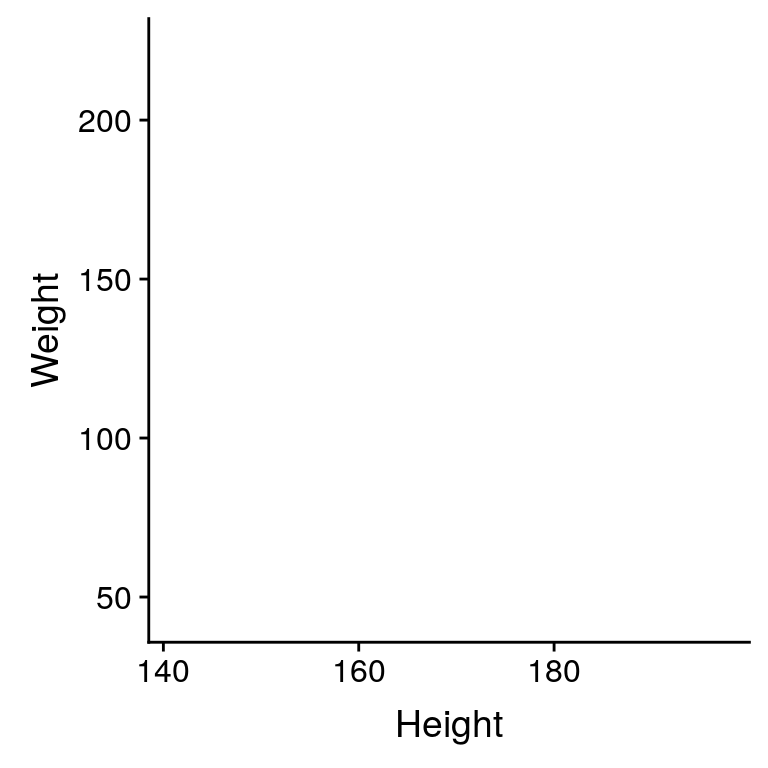
\includegraphics[height=0.5\textheight]{StatsThinking21_files/figure-latex/emptyPlot-1} \caption{Empty plot frame generated by ggplot()}\label{fig:emptyPlot}
\end{figure}

We next need to add a presentation of the data. The way that we tell
\texttt{ggplot} what to show is by adding various commands to the main
\texttt{ggplot()} command. In particular, we generally need to add a
\emph{geometry} or ``geom'', which specifies how the data will be
arranged in the plot. For example, to show each data point we can use
the \texttt{geom\_point()} geometry, as shown in Figure
\ref{fig:simpleGeom}. Each data point represents an individual row in
our \texttt{NHANES\_sample} dataset with each row corresponding to an
individual person in this dataset.

\begin{Shaded}
\begin{Highlighting}[]
\NormalTok{NHANES_sample }\OperatorTok\StringTok{ }
\StringTok{  }\KeywordTok{ggplot}\NormalTok{(}\KeywordTok{aes}\NormalTok{(}\DataTypeTok{x =}\NormalTok{ Height, }\DataTypeTok{y =}\NormalTok{ Weight)) }\OperatorTok{+}
\StringTok{  }\KeywordTok{geom_point}\NormalTok{()}
\end{Highlighting}
\end{Shaded}

\begin{figure}
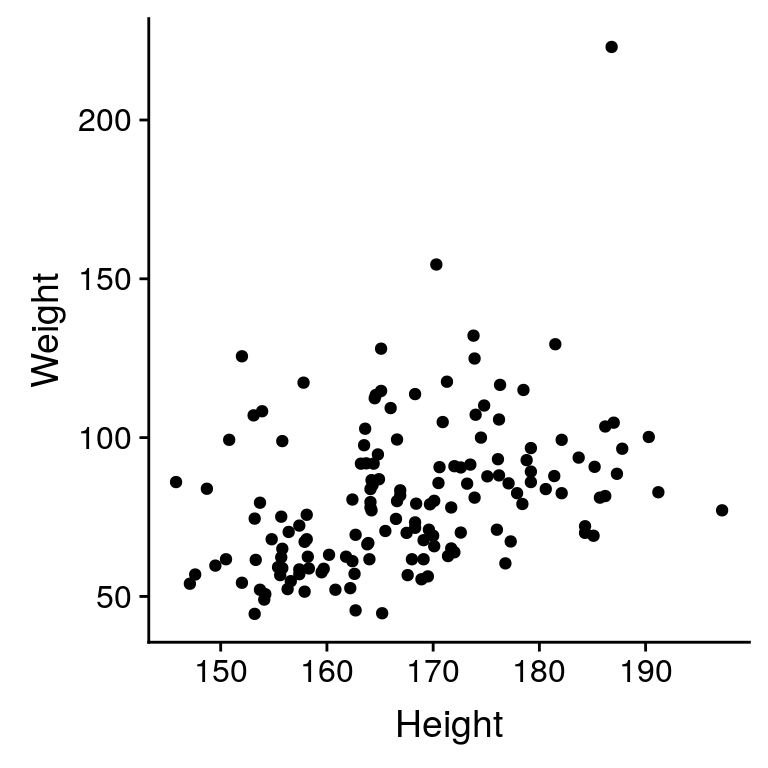
\includegraphics[height=0.5\textheight]{StatsThinking21_files/figure-latex/simpleGeom-1} \caption{Simple scatter plot}\label{fig:simpleGeom}
\end{figure}

Finally, we want to plot the points in separate colors depending on
their gender. We do this by simply adding a \emph{color} keyword to the
aesthetics, which tells the \texttt{geom\_point()} function to
separately color points by Gender. This is shown in Figure
\ref{fig:colorPoints}. This figure also shows an example of how we can
include multiple geometry layers in a single figure -- in this case, we
use \texttt{geom\_smooth()} to plot the lines that best describe the
relation between height and weight, separately by gender. The shading
around the lines reflects our confidence in the estimate at that point.

\begin{Shaded}
\begin{Highlighting}[]
\NormalTok{NHANES_sample }\OperatorTok\StringTok{ }
\StringTok{  }\KeywordTok{ggplot}\NormalTok{(}\KeywordTok{aes}\NormalTok{(}\DataTypeTok{x =}\NormalTok{ Height, }\DataTypeTok{y =}\NormalTok{ Weight, }\DataTypeTok{color =}\NormalTok{ Gender)) }\OperatorTok{+}
\StringTok{  }\KeywordTok{geom_point}\NormalTok{() }\OperatorTok{+}
\StringTok{  }\KeywordTok{geom_smooth}\NormalTok{(}\DataTypeTok{method =} \StringTok{"lm"}\NormalTok{)}
\end{Highlighting}
\end{Shaded}

\begin{figure}
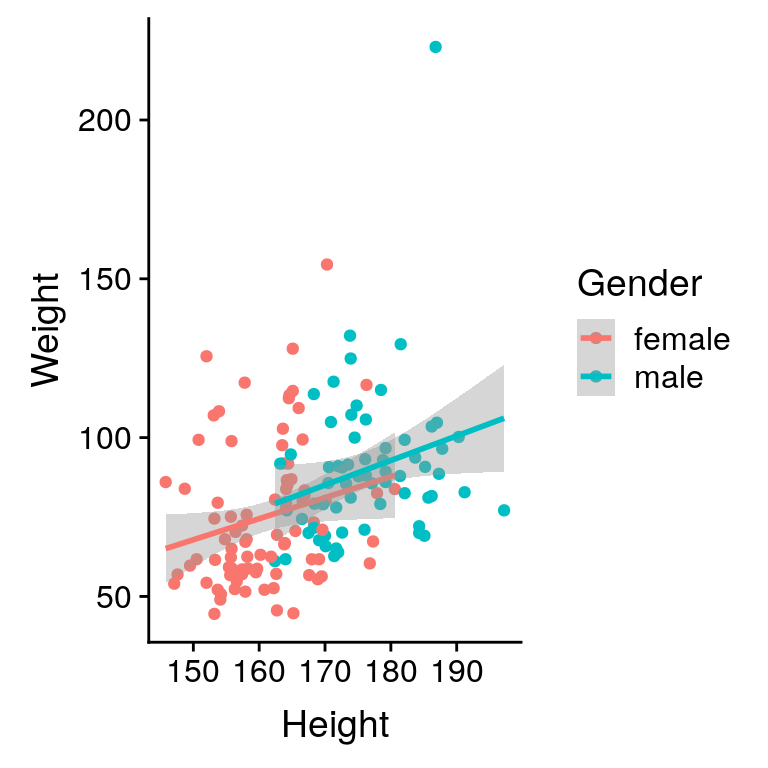
\includegraphics[height=0.5\textheight]{StatsThinking21_files/figure-latex/colorPoints-1} \caption{Scatterplot with points separately colored by Gender.}\label{fig:colorPoints}
\end{figure}

\section{Principles of good
visualization}\label{principles-of-good-visualization}

Many books have been written on effective visualization of data. There
are some principles that most of these authors agree on, while others
are more contentious. Here we summarize some of the major principles; if
you want to learn more, then some good resources are listed in the
\emph{Suggested Readings} section at the end of this chapter.

Here is our distillation of some important principles for data
visualization.

\subsection{Show the data and make them stand
out}\label{show-the-data-and-make-them-stand-out}

Let's say that I had performed a study that examined the relationship
between dental health and time spent flossing, and I would like to
visualize my data. Figure \ref{fig:dentalFigs} shows four possible
presentations of these data.

\begin{enumerate}
\def\labelenumi{\arabic{enumi}.}
\tightlist
\item
  In panel A, we don't actually show the data, just a line expressing
  the relationship between the data. This is clearly not optimal,
  because we can't actually see what the underlying data look like.
\end{enumerate}

Panels B-D show three possible outcomes from plotting the actual data,
where each plot shows a different way that the data could have been
generated.

\begin{enumerate}
\def\labelenumi{\arabic{enumi}.}
\setcounter{enumi}{1}
\tightlist
\item
  If we saw the plot in Panel B, we would probably be suspicious --
  rarely would real data follow such a precise pattern.\\
\item
  The data in Panel C, on the other hand, look like real data -- they
  show a general trend, but they are messy, as data in the world usually
  are.\\
\item
  The data in Panel D show us that the apparent relationship between the
  two variables is solely caused by one individual, who we would refer
  to as an \emph{outlier} because they fall so far outside of the
  pattern of the rest of the group. It should be clear that we probably
  don't want to conclude very much from an effect that is driven by one
  data point. This figure highlights why it is \emph{always} important
  to look at the raw data before putting too much faith in any summary
  of the data.
\end{enumerate}

\begin{figure}
\centering
\includegraphics{StatsThinking21_files/figure-latex/dentalFigs-1.pdf}
\caption{\label{fig:dentalFigs}Four different possible presentations of data
for the dental health example. Each point in the scatter plot represents
one data point in the dataset, and the line in each plot represents the
linear trend in the data.}
\end{figure}

\section{Maximize the data/ink ratio}\label{maximize-the-dataink-ratio}

Edward Tufte has proposed an idea called the data/ink ratio:

\[
data/ink\ ratio = \frac{amount\, of\, ink\, used\, on\, data}{total\, amount\, of\, ink}
\] The point of this is to minimize visual clutter and let the data show
through. For example, take the two presentations of the dental health
data in Figure \ref{fig:dataInkExample}. Both panels show the same data,
but panel A is much easier to apprehend, because of its relatively
higher data/ink ratio.

\begin{figure}
\includegraphics[height=0.5\textheight]{StatsThinking21_files/figure-latex/dataInkExample-1} \caption{An example of the same data plotted with two different data/ink ratios.}\label{fig:dataInkExample}
\end{figure}

\section{Avoid chartjunk}\label{avoid-chartjunk}

It's especially common to see presentations of data in the popular media
that are adorned with lots of visual elements that are thematically
related to the content but unrelated to the actual data. This is known
as \emph{chartjunk}, and should be avoided at all costs.

One good way to avoid chartjunk is to avoid using popular spreadsheet
programs to plot one's data. For example, the chart in Figure
\ref{fig:chartJunk} (created using Microsoft Excel) plots the relative
popularity of different religions in the United States. There are at
least three things wrong with this figure:

\begin{itemize}
\tightlist
\item
  it has graphics overlaid on each of the bars which have nothing to do
  with the actual data.
\item
  it has a distracting background texture.
\item
  it uses three-dimensional bars
\end{itemize}

\begin{figure}
\centering
\includegraphics{images/excel_chartjunk.png}
\caption{\label{fig:chartJunk}An example of chart junk.}
\end{figure}

\section{Avoid distorting the data}\label{avoid-distorting-the-data}

It's often possible to use visualization to distort the message of a
dataset. A very common one is use of different axis scaling to either
exaggerate or hide a pattern of data. For example, let's say that we are
interested in seeing whether rates of violent crime have changed in the
US. In Figure \ref{fig:crimePlotAxes}, we can see these data plotted in
ways that either make it look like crime has remained constant, or that
it has plummeted. The same data can tell two very different stories!

\begin{figure}
\includegraphics[height=0.5\textheight]{StatsThinking21_files/figure-latex/crimePlotAxes-1} \caption{Crime data from 1990 to 2014 plotted over time.  Panels A and B show the same data, but with different axis ranges. Data obtained from https://www.ucrdatatool.gov/Search/Crime/State/RunCrimeStatebyState.cfm}\label{fig:crimePlotAxes}
\end{figure}

One of the major controversies in statistical data visualization is how
to choose the Y axis, and in particular whether it should always include
zero. In his famous book ``How to lie with statistics'', Darrell Huff
argued strongly that one should always include the zero point in the Y
axis. On the other hand, Edward Tufte has argued against this:

\begin{quote}
``In general, in a time-series, use a baseline that shows the data not
the zero point; don't spend a lot of empty vertical space trying to
reach down to the zero point at the cost of hiding what is going on in
the data line itself.'' (from
\url{https://qz.com/418083/its-ok-not-to-start-your-y-axis-at-zero/})
\end{quote}

There are certainly cases where using the zero point makes no sense at
all. Let's say that we are interested in plotting body temperature for
an individual over time. In Figure \ref{fig:bodyTempAxis} we plot the
same (simulated) data with or without zero in the Y axis. It should be
obvious that by plotting these data with zero in the Y axis (Panel A) we
are wasting a lot of space in the figure, given that body temperature of
a living person could never go to zero! By including zero, we are also
making the apparent jump in temperature during days 21-30 much less
evident. In general, my inclination for line plots and scatterplots is
to use all of the space in the graph, unless the zero point is truly
important to highlight.

\begin{figure}
\includegraphics[height=0.5\textheight]{StatsThinking21_files/figure-latex/bodyTempAxis-1} \caption{Body temperature over time, plotted with or without the zero point in the Y axis.}\label{fig:bodyTempAxis}
\end{figure}

\section{The lie factor}\label{the-lie-factor}

Edward Tufte introduced the concept of the ``lie factor'' to describe
the degree to which physical differences in a visualization correspond
to the magnitude of the differences in the data. If a graphic has a lie
factor near 1, then it is appropriately representing the data, whereas
lie factors far from one reflect a distortion of the underlying data.

The lie factor supports the argument that one should always include the
zero point in a bar chart in many cases. In Figure
\ref{fig:barCharLieFactor} we plot the same data with and without zero
in the Y axis. In panel A, the proportional difference in area between
the two bars is exactly the same as the proportional difference between
the values (i.e.~lie factor = 1), whereas in Panel B (where zero is not
included) the proportional difference in area between the two bars is
roughly 2.8 times bigger than the proportional difference in the values,
and thus it visually exaggerates the size of the difference.

\begin{figure}
\includegraphics[height=0.5\textheight]{StatsThinking21_files/figure-latex/barCharLieFactor-1} \caption{Two bar charts with associated lie factors.}\label{fig:barCharLieFactor}
\end{figure}

\section{Remember human limitations}\label{remember-human-limitations}

Humans have both perceptual and cognitive limitations that can make some
visualizations very difficult to understand. It's always important to
keep these in mind when building a visualization.

\subsection{Perceptual limitations}\label{perceptual-limitations}

One important perceptual limitation that many people (including myself)
suffer from is color blindness. This can make it very difficult to
perceive the information in a figure (like the one in Figure
\ref{fig:badColors}) where there is only color contrast between the
elements but no brightness contrast. It is always helpful to use graph
elements that differ substantially in brightness and/or texture, in
addition to color. There are also
\href{http://www.cookbook-r.com/Graphs/Colors_(ggplot2)/\#a-colorblind-friendly-palette}{``colorblind-friendly''
pallettes} available for use in R

\begin{figure}
\includegraphics[height=0.5\textheight]{StatsThinking21_files/figure-latex/badColors-1} \caption{Example of a bad figure that relies solely on color contrast.}\label{fig:badColors}
\end{figure}

Even for people with perfect color vision, there are perceptual
limitations that can make some plots ineffective. This is one reason why
statisticians never use pie charts: It can be very difficult for humans
to apprehend differences in the volume of shapes. The piechart in Figure
\ref{fig:pieChart} (presenting the same data on religious affiliation
that we showed above) shows how tricky this can be.

\begin{figure}
\centering
\includegraphics{images/religion_piechart.png}
\caption{\label{fig:pieChart}An example of a pie chart, highlighting the
difficult in apprehending the relative volume of the different pie
slices.}
\end{figure}

This plot is terrible for several reasons. First, it requires
distinguishing a large number of colors from very small patches at the
bottom of the figure. Second, the visual perspective distorts the
relative numbers, such that the pie wedge for Catholic appears much
larger than the pie wedge for None, when in fact the number for None is
slightly larger (22.8 vs 20.8 percent), as was evident in Figure
\ref{fig:chartJunk}. Third, by separating the legend from the graphic,
it requires the viewer to hold information in their working memory in
order to map between the graphic and legend and to conduct many ``table
look-ups'' in order to continuously match the legend labels to the
visualization. And finally, it uses text that is far too small, making
it impossible to read without zooming in.

Plotting the data using a more reasonable approach (Figure
\ref{fig:religionBars}), we can see the pattern much more clearly. This
plot may not look as flashy as the pie chart generated using Excel, but
it's a much more effective and accurate representation of the data.

\begin{figure}
\includegraphics[height=0.5\textheight]{StatsThinking21_files/figure-latex/religionBars-1} \caption{A clearer presentation of the religious affiliation data (obtained from http://www.pewforum.org/religious-landscape-study/).}\label{fig:religionBars}
\end{figure}

This plot allows the viewer to make comparisons based on the the
\textbf{length} of the bars \textbf{along a common scale} (the y-axis).
Humans tend to be more accurate when decoding differences based on these
perceptual elements than based on area or color.

\section{Correcting for other
factors}\label{correcting-for-other-factors}

Often we are interested in plotting data where the variable of interest
is affected by other factors than the one we are interested in. For
example, let's say that we want to understand how the price of gasoline
has changed over time. Figure \ref{fig:gasPrices} shows historical gas
price data, plotted either with or without adjustment for inflation.
Whereas the unadjusted data show a huge increase, the adjusted data show
that this is mostly just reflective of inflation. Other examples where
one needs to adjust data for other factors include population size (as
we saw in the crime rate examples in an earlier chapter) and data
collected across different seasons.

\begin{figure}
\includegraphics[height=0.5\textheight]{StatsThinking21_files/figure-latex/gasPrices-1} \caption{The price of gasoline in the US from 1930 to 201 (obtained from http://www.thepeoplehistory.com/70yearsofpricechange.html) with or without correction for inflation (based on Consumer Price Index).}\label{fig:gasPrices}
\end{figure}

\section{Suggested readings and
videos}\label{suggested-readings-and-videos}

\begin{itemize}
\tightlist
\item
  \href{https://serialmentor.com/dataviz/}{\emph{Fundamentals of data
  visualization}}, by Claus Wilke
\item
  \emph{Visual Explanations}, by Edward Tufte
\item
  \emph{Visualizing Data}, by William S. Cleveland
\item
  \emph{Graph Design for the Eye and Mind}, by Stephen M. Kosslyn
\item
  \href{https://www.youtube.com/watch?v=fSgEeI2Xpdc\&feature=youtu.be}{\emph{How
  Humans See Data}}, by John Rauser
\end{itemize}

\chapter{Sampling}\label{sampling-1}

One of the foundational ideas in statistics is that we can make
inferences about an entire population based on a relatively small sample
of individuals from that population. In this chapter we will introduce
the concept of statistical sampling and discuss why it works.

Anyone living in the United States will be familiar with the concept of
sampling from the political polls that have become a central part of our
electoral process. In some cases, these polls can be incredibly accurate
at predicting the outcomes of elections. The best known example comes
from the 2008 and 2012 US Presidential elections, when the pollster Nate
Silver correctly predicted electoral outcomes for 49/50 states in 2008
and for all 50 states in 2012. Silver did this by combining data from 21
different polls, which vary in the degree to which they tend to lean
towards either the Republican or Democratic side. Each of these polls
included data from about 1000 likely voters -- meaning that Silver was
able to almost perfectly predict the pattern of votes of more than 125
million voters using data from only 21,000 people, along with other
knowledge (such as how those states have voted in the past).

\section{How do we sample?}\label{how-do-we-sample}

Our goal in sampling is to determine some feature of the full population
of interest, using just a small subset of the population. We do this
primarily to save time and effort -- why go to the trouble of measuring
every indivdual in the population when just a small sample is sufficient
to accurately estimate the variable of interest?

In the election example, the population is all voters, and the sample is
the set of 1000 individuals selected by the polling organization. The
way in which we select the sample is critical to ensuring that the
sample is \emph{representative} of the entire population, which is a
main goal of statistical sampling. It's easy to imagine a
non-representative sample; if a pollster only called individuals whose
names they had received from the local Democratic party, then it would
be unlikely that the results of the poll would be representative of the
population as a whole. In general, we would define a representative poll
as being one in which every member of the population has an equal chance
of being selected. When this fails, then we have to worry about whether
the statistic that we compute on the sample is \emph{biased} - that is,
whether its value is systematically different from the population value
(which we refer to as a \emph{parameter}). Keep in mind that we
generally don't know this population parameter, because if we did then
we wouldn't need to sample! But we will use examples where we have
access to the entire population, in order to explain some of the key
ideas.

It's important to also distinguish between two different ways of
sampling: with replacement versus without replacement. In sampling
\emph{with replacement}, after a member of the population has been
sampled, they are put back into the pool so that they can potentially be
sampled again. In \emph{sampling without replacement}, once a member has
been sampled they are not eligible to be sampled again. It's most common
to use sampling without replacement, but there will be some contexts in
which we will use sampling with replacement, as when we discuss a
technique called \emph{bootstrapping} in Chapter
\ref{resampling-and-simulation}.

\section{Sampling error}\label{sampling-error}

Regardless of how representative our sample is, it's likely that the
statistic that we compute from the sample is going to differ at least
slightly from the population parameter. We refer to this as
\emph{sampling error}. The value of our statistical estimate will also
vary from sample to sample; we refer to this distribution of our
statistic across samples as the \emph{sampling distribution}.

Sampling error is directly related to the quality of our measurement of
the population. Clearly we want the estimates obtained from our sample
to be as close as possible to the true value of the population
parameter. However, even if our statistic is unbiased (that is, in the
long run we expect it to have the same value as the population
parameter), the value for any particular estimate will differ from the
population estimate, and those differences will be greater when the
sampling error is greater. Thus, reducing sampling error is an important
step towards better measurement.

We will use the NHANES dataset as an example; we are going to assume
that NHANES is the entire population, and then we will draw random
samples from the population. We will have more to say in the next
chapter about exactly how the generation of ``random'' samples works in
a computer.

\begin{Shaded}
\begin{Highlighting}[]
\CommentTok{# load the NHANES data library}
\KeywordTok{library}\NormalTok{(NHANES)}

\CommentTok{# create a NHANES dataset without duplicated IDs }
\NormalTok{NHANES <-}
\StringTok{  }\NormalTok{NHANES }\OperatorTok
\StringTok{  }\KeywordTok{distinct}\NormalTok{(ID, }\DataTypeTok{.keep_all =} \OtherTok{TRUE}\NormalTok{) }

\CommentTok{#create a dataset of only adults}
\NormalTok{NHANES_adult <-}\StringTok{ }
\StringTok{  }\NormalTok{NHANES }\OperatorTok
\StringTok{  }\KeywordTok{filter}\NormalTok{( }
    \OperatorTok{!}\KeywordTok{is.na}\NormalTok{(Height), }
\NormalTok{    Age }\OperatorTok{>=}\StringTok{ }\DecValTok{18}
\NormalTok{  )}

\CommentTok{#print the NHANES population mean and standard deviation of adult height}
\KeywordTok{sprintf}\NormalTok{(}
  \StringTok{"Population height: mean = %.2f"}\NormalTok{,}
  \KeywordTok{mean}\NormalTok{(NHANES_adult}\OperatorTok{$}\NormalTok{Height)}
\NormalTok{)}
\end{Highlighting}
\end{Shaded}

\begin{verbatim}
## [1] "Population height: mean = 168.35"
\end{verbatim}

\begin{Shaded}
\begin{Highlighting}[]
\KeywordTok{sprintf}\NormalTok{(}
  \StringTok{"Population height: std deviation = %.2f"}\NormalTok{,}
  \KeywordTok{sd}\NormalTok{(NHANES_adult}\OperatorTok{$}\NormalTok{Height)}
\NormalTok{)}
\end{Highlighting}
\end{Shaded}

\begin{verbatim}
## [1] "Population height: std deviation = 10.16"
\end{verbatim}

In this example, we know the adult population mean and standard
deviation for height because we are assuming that the NHANES dataset
contains the entire population of adults. Now let's take a single sample
of 50 individuals from the NHANES population, and compare the resulting
statistics to the population parameters.

\begin{Shaded}
\begin{Highlighting}[]
\CommentTok{# sample 50 individuals from NHANES dataset}
\NormalTok{exampleSample <-}\StringTok{ }
\StringTok{  }\NormalTok{NHANES_adult }\OperatorTok\StringTok{ }
\StringTok{  }\KeywordTok{sample_n}\NormalTok{(}\DecValTok{50}\NormalTok{)}

\CommentTok{#print the sample mean and standard deviation of adult height}
\KeywordTok{sprintf}\NormalTok{(}
  \StringTok{'Sample height: mean = %.2f'}\NormalTok{,}
  \KeywordTok{mean}\NormalTok{(exampleSample}\OperatorTok{$}\NormalTok{Height)}
\NormalTok{  )}
\end{Highlighting}
\end{Shaded}

\begin{verbatim}
## [1] "Sample height: mean = 169.46"
\end{verbatim}

\begin{Shaded}
\begin{Highlighting}[]
\KeywordTok{sprintf}\NormalTok{(}
  \StringTok{'Sample height: std deviation = %.2f'}\NormalTok{,}
  \KeywordTok{sd}\NormalTok{(exampleSample}\OperatorTok{$}\NormalTok{Height)}
\NormalTok{)}
\end{Highlighting}
\end{Shaded}

\begin{verbatim}
## [1] "Sample height: std deviation = 10.07"
\end{verbatim}

The sample mean and standard deviation are similar but not exactly equal
to the population values. Now let's take a large number of samples of 50
individuals, compute the mean for each sample, and look at the resulting
sampling distribution of means. We have to decide how many samples to
take in order to do a good job of estimating the sampling distribution
-- in this case, let's take 5000 samples so that we are really confident
in the answer. Note that simulations like this one can sometimes take a
few minutes to run, and might make your computer huff and puff. The
histogram in Figure \ref{fig:samplePlot} shows that the means estimated
for each of the samples of 50 individuals vary somewhat, but that
overall they are centered around the population mean.

\begin{Shaded}
\begin{Highlighting}[]
\CommentTok{# compute sample means across 5000 samples from NHANES data}
\NormalTok{sampSize <-}\StringTok{ }\DecValTok{50} \CommentTok{# size of sample}
\NormalTok{nsamps <-}\StringTok{ }\DecValTok{5000} \CommentTok{# number of samples we will take}

\CommentTok{# set up variable to store all of the results}
\NormalTok{sampMeans <-}\StringTok{ }\KeywordTok{array}\NormalTok{(}\OtherTok{NA}\NormalTok{, nsamps)}

\CommentTok{# Loop through and repeatedly sample and compute the mean}
\ControlFlowTok{for}\NormalTok{ (i }\ControlFlowTok{in} \DecValTok{1}\OperatorTok{:}\NormalTok{nsamps) \{}
\NormalTok{  NHANES_sample <-}\StringTok{ }\KeywordTok{sample_n}\NormalTok{(NHANES_adult, sampSize)}
\NormalTok{  sampMeans[i] <-}\StringTok{ }\KeywordTok{mean}\NormalTok{(NHANES_sample}\OperatorTok{$}\NormalTok{Height)}
\NormalTok{\}}

\NormalTok{sampdataDf <-}\StringTok{ }\KeywordTok{tibble}\NormalTok{(}\DataTypeTok{mean =}\NormalTok{ sampMeans)}

\KeywordTok{sprintf}\NormalTok{(}
  \StringTok{"Average sample mean = %.2f"}\NormalTok{,}
  \KeywordTok{mean}\NormalTok{(sampMeans)}
\NormalTok{)}
\end{Highlighting}
\end{Shaded}

\begin{verbatim}
## [1] "Average sample mean = 168.33"
\end{verbatim}

\begin{Shaded}
\begin{Highlighting}[]
\NormalTok{sampMeans_df <-}\StringTok{ }\KeywordTok{tibble}\NormalTok{(}\DataTypeTok{sampMeans =}\NormalTok{ sampMeans)}
\end{Highlighting}
\end{Shaded}

\begin{figure}
\includegraphics[height=0.5\textheight]{StatsThinking21_files/figure-latex/samplePlot-1} \caption{The blue histogram shows the sampling distribution of the mean over 5000 random samples from the NHANES dataset.  The histogram for the full dataset is shown in gray for reference.}\label{fig:samplePlot}
\end{figure}

\section{Standard error of the mean}\label{standard-error-of-the-mean}

Later in the course it will become essential to be able to characterize
how variable our samples are, in order to make inferences about the
sample statistics. For the mean, we do this using a quantity called the
\emph{standard error} of the mean (SEM), which one can think of as the
standard deviation of the sampling distribution. If we know the
population standard deviation, then we can compute the standard error
using:

\[
SEM = \frac{\sigma}{\sqrt{n}}
\] where \(n\) is the size of the sample. We don't usually know
\(\sigma\) (the population standard deviation), so instead we would
usually plug in our estimate of \(\sigma\), which is the standard
deviation computed on the sample (\(\hat{\sigma}\)):

\[
SEM = \frac{\hat{\sigma}}{\sqrt{n}}
\]

However, we have to be careful about computing SEM using the estimated
standard deviation if our sample is small (less than about 30).

Because we have many samples from the NHANES population and we actually
know the population parameter, we can confirm that the SEM estimated
using the population parameter is very close to the observed standard
deviation of the samples that we took from the NHANES dataset.

\begin{Shaded}
\begin{Highlighting}[]
\CommentTok{# compare standard error based on population to standard deviation }
\CommentTok{# of sample means}

\KeywordTok{sprintf}\NormalTok{(}
  \StringTok{'Estimated standard error based on population SD: %.2f'}\NormalTok{,}
  \KeywordTok{sd}\NormalTok{(NHANES_adult}\OperatorTok{$}\NormalTok{Height)}\OperatorTok{/}\KeywordTok{sqrt}\NormalTok{(sampSize)}
\NormalTok{)}
\end{Highlighting}
\end{Shaded}

\begin{verbatim}
## [1] "Estimated standard error based on population SD: 1.44"
\end{verbatim}

\begin{Shaded}
\begin{Highlighting}[]
\KeywordTok{sprintf}\NormalTok{(}
  \StringTok{'Standard deviation of sample means = %.2f'}\NormalTok{,}
  \KeywordTok{sd}\NormalTok{(sampMeans)}
\NormalTok{)}
\end{Highlighting}
\end{Shaded}

\begin{verbatim}
## [1] "Standard deviation of sample means = 1.43"
\end{verbatim}

The formula for the standard error of the mean says that the quality of
our measurement involves two quantities: the population variability, and
the size of our sample. Of course, because the sample size is the
denominator in the formula for SEM, a larger sample size will yield a
smaller SEM when holding the population variability constant. We have no
control over the population variability, but we \emph{do} have control
over the sample size. Thus, if we wish to improve our sample statistics
(by reducing their sampling variability) then we should use larger
samples. However, the formula also tells us something very fundamental
about statistical sampling -- namely, that the utility of larger samples
diminishes with the square root of the sample size. This means that
doubling the sample size will \emph{not} double the quality of the
statistics; rather, it will improve it by a factor of \(\sqrt{2}\). In
Section \ref(statistical-power) we will discuss statistical power, which
is intimately tied to this idea.

\section{The Central Limit Theorem}\label{the-central-limit-theorem}

The Central Limit Theorem tells us that as sample sizes get larger, the
sampling distribution of the mean will become normally distributed,
\emph{even if the data within each sample are not normally distributed}.

We can also see this in real data. Let's work with the variable
AlcoholYear in the NHANES distribution, which is highly skewed, as shown
in Figure \ref{fig:alcoholYearDist}.

\begin{figure}
\includegraphics[height=0.5\textheight]{StatsThinking21_files/figure-latex/alcoholYearDist-1} \caption{Distribution of the variable AlcoholYear in the NHANES dataset, which reflects the number of days that the individual drank in a year.}\label{fig:alcoholYearDist}
\end{figure}

This distribution is, for lack of a better word, funky -- and definitely
not normally distributed. Now let's look at the sampling distribution of
the mean for this variable. Figure \ref{fig:alcDist50} shows the
sampling distribution for this variable, which is obtained by repeatedly
drawing samples of size 50 from the NHANES dataset and taking the mean.
Despite the clear non-normality of the original data, the sampling
distribution is remarkably close to the normal.

\begin{figure}
\includegraphics[height=0.5\textheight]{StatsThinking21_files/figure-latex/alcDist50-1} \caption{The sampling distribution of the mean for AlcoholYear in the NHANES dataset, obtained by drawing repeated samples of size 50, in blue.  The normal distribution with the same mean and standard deviation is shown in red.}\label{fig:alcDist50}
\end{figure}

\section{Confidence intervals}\label{confidence-intervals}

Most people are familiar with the idea of a ``margin of error'' for
political polls. These polls usually try to provide an answer that is
accurate within +/- 3 percent. For example, when a candidate is
estimated to win an election by 9 percentage points with a margin of
error of 3, the percentage by which they will win is estimated to fall
within 6-12 percentage points. In statistics we refer to this range of
values as the \emph{confidence interval}, which provides a measure of
our degree of uncertainty about how close our estimate is to the
population parameter. The larger the condidence interval, the greater
our uncertainty.

We saw in the previous section that with sufficient sample size, the
sampling distribution of the mean is normally distributed, and that the
standard error describes the standard deviation of this sampling
distribution. Using this knowledge, we can ask: What is the range of
values within which we would expect to capture 95\% of all estimates of
the mean? To answer this, we can use the normal distribution, for which
we know the values between which we expect 95\% of all sample means to
fall. Specifically, we use the \emph{quantile} function for the normal
distribution (\texttt{qnorm()} in R) to determine the values of the
normal distribution that fall at the 2.5\% and 97.5\% points in the
distribution. We choose these points because we want to find the 95\% of
values in the center of the distribution, so we need to cut off 2.5\% on
each end in order to end up with 95\% in the middle. Figure
\ref{fig:normalCutoffs} shows that this occurs for \(Z \pm 1.96\).

\textbackslash{}begin\{figure\}
\includegraphics[height=0.5\textheight]{StatsThinking21_files/figure-latex/normalCutoffs-1}
\textbackslash{}caption\{Normal distribution, with the orange section in
the center denoting the range in which we expect 95\% of all values to
fall. The green sections show the portions of the distribution that are
more extreme, which we would expect to occur less than 5\% of the
time.\}\label{fig:normalCutoffs} \textbackslash{}end\{figure\}

Using these cutoffs, we can create a confidence interval for the
estimate of the mean:

\[
CI_{95\%} = \bar{X} \pm 1.96*SEM
\]

Let's compute the confidence interval for the NHANES height data,

\begin{Shaded}
\begin{Highlighting}[]
\CommentTok{# compute confidence intervals}

\NormalTok{NHANES_sample <-}\StringTok{ }\KeywordTok{sample_n}\NormalTok{(NHANES_adult,}\DecValTok{250}\NormalTok{)}

\NormalTok{sample_summary <-}\StringTok{ }\NormalTok{NHANES_sample }\OperatorTok
\StringTok{    }\KeywordTok{summarize}\NormalTok{(}\DataTypeTok{mean=}\KeywordTok{mean}\NormalTok{(Height),}
            \DataTypeTok{sem=}\KeywordTok{sd}\NormalTok{(Height)}\OperatorTok{/}\KeywordTok{sqrt}\NormalTok{(sampSize)) }\OperatorTok
\StringTok{    }\KeywordTok{mutate}\NormalTok{(}\DataTypeTok{CI_lower=}\NormalTok{mean}\OperatorTok{-}\FloatTok{1.96}\OperatorTok{*}\NormalTok{sem,}
           \DataTypeTok{CI_upper=}\NormalTok{mean}\OperatorTok{+}\FloatTok{1.96}\OperatorTok{*}\NormalTok{sem)}
\KeywordTok{pander}\NormalTok{(sample_summary)}
\end{Highlighting}
\end{Shaded}

\begin{longtable}[]{@{}cccc@{}}
\toprule
\begin{minipage}[b]{0.12\columnwidth}\centering\strut
mean\strut
\end{minipage} & \begin{minipage}[b]{0.10\columnwidth}\centering\strut
sem\strut
\end{minipage} & \begin{minipage}[b]{0.14\columnwidth}\centering\strut
CI\_lower\strut
\end{minipage} & \begin{minipage}[b]{0.14\columnwidth}\centering\strut
CI\_upper\strut
\end{minipage}\tabularnewline
\midrule
\endhead
\begin{minipage}[t]{0.12\columnwidth}\centering\strut
166.869\strut
\end{minipage} & \begin{minipage}[t]{0.10\columnwidth}\centering\strut
1.446\strut
\end{minipage} & \begin{minipage}[t]{0.14\columnwidth}\centering\strut
164.036\strut
\end{minipage} & \begin{minipage}[t]{0.14\columnwidth}\centering\strut
169.702\strut
\end{minipage}\tabularnewline
\bottomrule
\end{longtable}

Confidence intervals are notoriously confusing, primarily because they
don't mean what we would hope they mean. It seems natural to think that
the 95\% confidence interval tells us that there is a 95\% chance that
the population mean falls within the interval. However, as we will see
throughout the course, concepts in statsitics often don't mean what we
think they should mean. In the case of confidence intervals, we can't
interpret them in this way because the population parameter has a fixed
value -- it either is or isn't in the interval. The proper
interpretation of the 95\% confidence interval is that it is the
interval that will capture the true population mean 95\% of the time. We
can confirm this by resampling the NHANES data repeatedly and counting
how often the interval contains the true population mean.

\begin{Shaded}
\begin{Highlighting}[]
\CommentTok{# compute how often the confidence interval contains the true population mean}
\NormalTok{nsamples <-}\StringTok{ }\DecValTok{2500}
\NormalTok{sampSize <-}\StringTok{ }\DecValTok{100}

\NormalTok{ci_contains_mean <-}\StringTok{ }\KeywordTok{array}\NormalTok{(}\OtherTok{NA}\NormalTok{,nsamples)}

\ControlFlowTok{for}\NormalTok{ (i }\ControlFlowTok{in} \DecValTok{1}\OperatorTok{:}\NormalTok{nsamples) \{}
\NormalTok{  NHANES_sample <-}\StringTok{ }\KeywordTok{sample_n}\NormalTok{(NHANES_adult, sampSize)}
\NormalTok{  sample_summary <-}\StringTok{ }
\StringTok{    }\NormalTok{NHANES_sample }\OperatorTok
\StringTok{    }\KeywordTok{summarize}\NormalTok{(}
      \DataTypeTok{mean =} \KeywordTok{mean}\NormalTok{(Height),}
      \DataTypeTok{sem =} \KeywordTok{sd}\NormalTok{(Height) }\OperatorTok{/}\StringTok{ }\KeywordTok{sqrt}\NormalTok{(sampSize)}
\NormalTok{    ) }\OperatorTok
\StringTok{    }\KeywordTok{mutate}\NormalTok{(}
      \DataTypeTok{CI_upper =}\NormalTok{ mean }\OperatorTok{+}\StringTok{ }\FloatTok{1.96} \OperatorTok{*}\StringTok{ }\NormalTok{sem,}
      \DataTypeTok{CI_lower =}\NormalTok{ mean }\OperatorTok{-}\StringTok{ }\FloatTok{1.96} \OperatorTok{*}\StringTok{ }\NormalTok{sem}
\NormalTok{    )}
\NormalTok{  ci_contains_mean[i] <-}\StringTok{ }
\StringTok{    }\NormalTok{(sample_summary}\OperatorTok{$}\NormalTok{CI_upper }\OperatorTok{>}\StringTok{ }\KeywordTok{mean}\NormalTok{(NHANES_adult}\OperatorTok{$}\NormalTok{Height)) }\OperatorTok{&}\StringTok{ }
\StringTok{    }\NormalTok{(sample_summary}\OperatorTok{$}\NormalTok{CI_lower }\OperatorTok{<}\StringTok{ }\KeywordTok{mean}\NormalTok{(NHANES_adult}\OperatorTok{$}\NormalTok{Height))}
\NormalTok{\}}

\KeywordTok{sprintf}\NormalTok{(}
  \StringTok{'proportion of confidence intervals containing population mean: %.3f'}\NormalTok{,}
  \KeywordTok{mean}\NormalTok{(ci_contains_mean)}
\NormalTok{)}
\end{Highlighting}
\end{Shaded}

\begin{verbatim}
## [1] "proportion of confidence intervals containing population mean: 0.953"
\end{verbatim}

This confirms that the confidence interval does indeed capture the
population mean about 95\% of the time.

\section{Suggested readings}\label{suggested-readings-4}

\begin{itemize}
\tightlist
\item
  \emph{The Signal and the Noise: Why So Many Predictions Fail - But
  Some Don't}, by Nate Silver
\end{itemize}

\chapter{Resampling and simulation}\label{resampling-and-simulation}

The use of computer simulations has become an essential aspect of modern
statistics. For example, one of the most important books in practical
computer science, called \emph{Numerical Recipes}, says the following:

\begin{quote}
``Offered the choice between mastery of a five-foot shelf of analytical
statistics books and middling ability at performing statistical Monte
Carlo simulations, we would surely choose to have the latter skill.''
\end{quote}

In this chapter we will introduce the concept of a Monte Carlo
simulation and discuss how they can be used to perform statistical
analyses.

\section{Monte Carlo simulation}\label{monte-carlo-simulation}

The concept of Monte Carlo simulation was devised by the mathematicians
Stan Ulam and Nicholas Metropolis, who were working to develop an atomic
weapon as part of the Manhattan Project
(\url{https://en.wikipedia.org/wiki/Manhattan_Project}). They needed to
compute the average distance that a neutron would travel in a substance
before it collided with an atomic nucleus, but they could not compute
this using standard mathematics. Ulam realized that these computations
could be simulated using random numbers, just like a casino game. In a
casino game, numbers are drawn at random; to estimate the probability of
a specific outcome, you could play the game hundreds of times. Ulam's
uncle had gambled at the Monte Carlo casino in Monaco, which is
apparently where the name came from for this new technique.

There are four steps to performing a Monte Carlo simulation:

\begin{enumerate}
\def\labelenumi{\arabic{enumi}.}
\tightlist
\item
  Define a domain of possible values
\item
  Generate random numbers within that domain from a probability
  distribution
\item
  Perform a computation using the random numbers
\item
  Combine the results across many repetitions
\end{enumerate}

As an example, let's say that I want to figure out how much time to
allow for an in-class quiz. Say that we know that the distribution of
quiz completion times is normal, with mean of 5 mins and standard
deviation of 1 min. Given this, how long does the test period need to be
so that we expect everyone to finish 99\% of the time? There are two
ways to solve this problem. The first is to calculate the answer using a
mathematical theory known as the statistics of extreme values. However,
this is quite complicated mathematically. Alternatively, we could use
Monte Carlo simulation. To do this, we need to generate random samples
from a normal distribution.

\section{Randomness in statistics}\label{randomness-in-statistics}

The term ``random'' is often used colloquiually to refer to things that
are bizarre or unexpected, but in statistics the term has a very
specific meaning: A process is \emph{random} if it is unpredictable. For
example, if I flip a fair coin 10 times, the value of the outcome on one
flip does not provide me with any information that lets me predict the
outcome on the next flip. It's important to note that the fact that
something is unpredictable doesn't necessarily mean that it is not
deterministic. For example, when we flip a coin, the outcome of the flip
is determined by the laws of physics; if we knew all of the conditions
in enough detail, we should be able to predict the outcome of the flip.
However, many factors combine to make the outcome of the coin flip
unpredictable in practice.

Psychologists have shown that humans actually have a fairly bad sense of
randomness. First, we tend to see patterns when they don't exist. In the
extreme, this leads to the phenomenon of \emph{pareidolia}, in which
people will perceive familiar objects within random patterns (such as
perceiving a cloud as a human face or seeing the Virgin Mary in a piece
of toast). Second, humans tend to think of random processes as
self-correcting, which leads us to expect that we are ``due for a win''
after losing many rounds in a game, a phenonenon known as the
``gambler's fallacy''.

\section{Generating random numbers}\label{generating-random-numbers}

Running a Monte Carlo simulation requires that we generate random
numbers. Generating truly random numbers (i.e.~numbers that are
completely unpredictable) is only possible through physical processes,
such as the decay of atoms or the rolling of dice, which are difficult
to obtain and/or too slow to be useful for computer simulation (though
they can be obtained from the
\href{https://www.nist.gov/programs-projects/nist-randomness-beacon\%5D}{NIST
Randomness Beacon}).

In general, instead of truly random numbers we use \emph{pseudo-random}
numbers generated using a computer algorithm; these numbers will seem
random in the sense that they are difficult to predict, but the series
of numbers will actually repeat at some point. For example, the random
number generator used in R will repeate after \(2^{19937} - 1\) numbers.
That's far more than the number of seconds in the history of the
universe, and we generally think that this is fine for most purposes in
statistical analysis.

In R, there is a function to generate random numbers for each of the
major probability distributions, such as:

\begin{itemize}
\tightlist
\item
  \texttt{runif()} - uniform distribution (all values between 0 and 1
  equally)
\item
  \texttt{rnorm()} - normal distribution
\item
  \texttt{rbinom()} - binomial distribution (e.g.~rolling the dice, coin
  flips)
\end{itemize}

Figure \ref{fig:rngExamples} shows examples of numbers generated using
the \texttt{runif()} and \texttt{rnorm()} functions, generated using the
following code:

\begin{Shaded}
\begin{Highlighting}[]
\NormalTok{p1 <-}
\StringTok{  }\KeywordTok{tibble}\NormalTok{(}
    \DataTypeTok{x =} \KeywordTok{runif}\NormalTok{(}\DecValTok{10000}\NormalTok{)}
\NormalTok{  ) }\OperatorTok\StringTok{ }
\StringTok{  }\KeywordTok{ggplot}\NormalTok{((}\KeywordTok{aes}\NormalTok{(x))) }\OperatorTok{+}
\StringTok{  }\KeywordTok{geom_histogram}\NormalTok{(}\DataTypeTok{bins =} \DecValTok{100}\NormalTok{) }\OperatorTok{+}\StringTok{ }
\StringTok{  }\KeywordTok{labs}\NormalTok{(}\DataTypeTok{title =} \StringTok{"Uniform"}\NormalTok{)}

\NormalTok{p2 <-}
\StringTok{  }\KeywordTok{tibble}\NormalTok{(}
    \DataTypeTok{x =} \KeywordTok{rnorm}\NormalTok{(}\DecValTok{10000}\NormalTok{)}
\NormalTok{  ) }\OperatorTok\StringTok{ }
\StringTok{  }\KeywordTok{ggplot}\NormalTok{(}\KeywordTok{aes}\NormalTok{(x)) }\OperatorTok{+}
\StringTok{  }\KeywordTok{geom_histogram}\NormalTok{(}\DataTypeTok{bins =} \DecValTok{100}\NormalTok{) }\OperatorTok{+}
\StringTok{  }\KeywordTok{labs}\NormalTok{(}\DataTypeTok{title =} \StringTok{"Normal"}\NormalTok{)}

\KeywordTok{plot_grid}\NormalTok{(p1, p2, }\DataTypeTok{ncol =} \DecValTok{3}\NormalTok{)}
\end{Highlighting}
\end{Shaded}

\begin{figure}
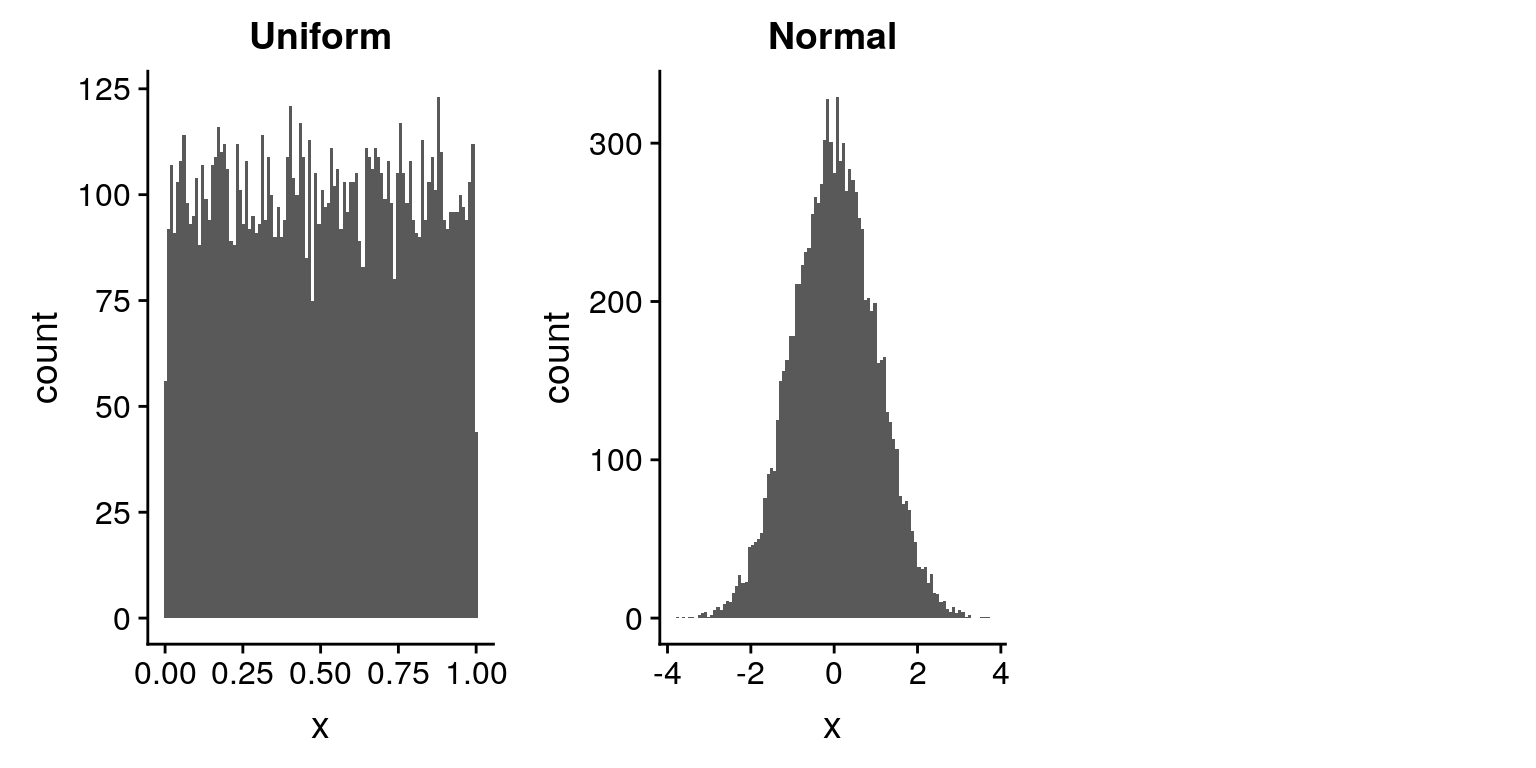
\includegraphics[height=0.5\textheight]{StatsThinking21_files/figure-latex/rngExamples-1} \caption{Examples of random numbers generated from a uniform (left) or normal (right) distribution.}\label{fig:rngExamples}
\end{figure}

You can also generate random numbers for any distribution if you have a
\emph{quantile} function for the distribution. This is the inverse of
the cumulative distribution function; instead of identifying the
cumulative probabilities for a set of values, the quantile function
identifies the values for a set of cumulative probabilities. Using the
quantile function, we can generate random numbers from a uniform
distribution, and then map those into the distribution of interest via
its quantile function.

By default, R will generate a different set of random numbers every time
you run one of the random number generator functions described above.
However, it is also possible to generate exactly the same set of random
numbers, by setting what is called the \emph{random seed} to a specific
value. We will do this in many of the examples in this book, in order to
make sure that the examples are reproducible.

\begin{Shaded}
\begin{Highlighting}[]
\CommentTok{# if we run the rnorm() command twice, it will give us different sets of pseudorandom numbers each time}
\KeywordTok{print}\NormalTok{(}\KeywordTok{rnorm}\NormalTok{(}\DataTypeTok{n =} \DecValTok{5}\NormalTok{))}
\end{Highlighting}
\end{Shaded}

\begin{verbatim}
## [1]  1.48  0.18  0.21 -0.15 -1.72
\end{verbatim}

\begin{Shaded}
\begin{Highlighting}[]
\KeywordTok{print}\NormalTok{(}\KeywordTok{rnorm}\NormalTok{(}\DataTypeTok{n =} \DecValTok{5}\NormalTok{))}
\end{Highlighting}
\end{Shaded}

\begin{verbatim}
## [1] -0.691 -2.231  0.391  0.029 -0.647
\end{verbatim}

\begin{Shaded}
\begin{Highlighting}[]
\CommentTok{# if we set the random seed to the same value each time, then it will give us the same series of pseudorandom numbers each time.}
\KeywordTok{set.seed}\NormalTok{(}\DecValTok{12345}\NormalTok{)}
\KeywordTok{print}\NormalTok{(}\KeywordTok{rnorm}\NormalTok{(}\DataTypeTok{n =} \DecValTok{5}\NormalTok{))}
\end{Highlighting}
\end{Shaded}

\begin{verbatim}
## [1]  0.59  0.71 -0.11 -0.45  0.61
\end{verbatim}

\begin{Shaded}
\begin{Highlighting}[]
\KeywordTok{set.seed}\NormalTok{(}\DecValTok{12345}\NormalTok{)}
\KeywordTok{print}\NormalTok{(}\KeywordTok{rnorm}\NormalTok{(}\DataTypeTok{n =} \DecValTok{5}\NormalTok{))}
\end{Highlighting}
\end{Shaded}

\begin{verbatim}
## [1]  0.59  0.71 -0.11 -0.45  0.61
\end{verbatim}

\section{Using Monte Carlo
simulation}\label{using-monte-carlo-simulation}

Let's go back to our example of exam finishing times. Let's say that I
administer three quizzes and record the finishing times for each student
for each exam, which might look like the distributions presented in
Figure \ref{fig:finishingTimes}.

\begin{figure}
\includegraphics[height=0.5\textheight]{StatsThinking21_files/figure-latex/finishingTimes-1} \caption{Simulated finishing time distributions.}\label{fig:finishingTimes}
\end{figure}

However, what we really want to know is not what the distribution of
finishing times looks like, but rather what the distribution of the
\emph{longest} finishing time for each quiz looks like. To do this, we
can simulate a large number of quizzes (using the assumption that the
finishing times are distributed normally, as stated above); for each of
these simulated quizzes, we can record the longest finishing time. To do
this, we create a new function in R called \texttt{sampleMax()} which
simulates a sample of the appropriate size (i.e.~the number of students
in the class) from the appropriate distribution (i.e., normal), and
returns the maximum value in the sample. We then repeat this simulation
a large number of times (5000 should be enough) using the
\texttt{replicate()} function, which will store all of the outputs into
a single variable. The distribution of finishing times is shown in
Figure \ref{fig:finishTimeSim}.

\begin{Shaded}
\begin{Highlighting}[]
\CommentTok{# sample maximum value 5000 times and compute 99th percentile}
\NormalTok{nRuns <-}\StringTok{ }\DecValTok{5000}
\NormalTok{sampSize <-}\StringTok{ }\DecValTok{150}

\NormalTok{sampleMax <-}\StringTok{ }\ControlFlowTok{function}\NormalTok{(}\DataTypeTok{sampSize =} \DecValTok{150}\NormalTok{) \{}
\NormalTok{  samp <-}\StringTok{ }\KeywordTok{rnorm}\NormalTok{(sampSize, }\DataTypeTok{mean =} \DecValTok{5}\NormalTok{, }\DataTypeTok{sd =} \DecValTok{1}\NormalTok{)}
  \KeywordTok{return}\NormalTok{(}\KeywordTok{max}\NormalTok{(samp))}
\NormalTok{\}}

\NormalTok{maxTime <-}\StringTok{ }\KeywordTok{replicate}\NormalTok{(nRuns, }\KeywordTok{sampleMax}\NormalTok{())}

\NormalTok{cutoff <-}\StringTok{ }\KeywordTok{quantile}\NormalTok{(maxTime, }\FloatTok{0.99}\NormalTok{)}
\KeywordTok{sprintf}\NormalTok{(}\StringTok{"99th percentile of maxTime distribution: %.2f"}\NormalTok{, cutoff)}
\end{Highlighting}
\end{Shaded}

\begin{verbatim}
## [1] "99th percentile of maxTime distribution: 8.81"
\end{verbatim}

\begin{figure}
\includegraphics[height=0.5\textheight]{StatsThinking21_files/figure-latex/finishTimeSim-1} \caption{Distribution of maximum finishing times across simulations.}\label{fig:finishTimeSim}
\end{figure}

This shows that the 99th percentile of the finishing time distribution
falls at 8.81, meaning that if we were to give that much time for the
quiz, then everyone should finish 99\% of the time. It's always
important to remember that our assumptions matter -- if they are wrong,
then the results of the simulation are useless. In this case, we assumed
that the finishing time distribution was normally distributed with a
particular mean and standard deviation; if these assumptions are
incorrect (and they almost certainly are), then the true answer could be
very different.

\section{Using simulation for statistics: The
bootstrap}\label{using-simulation-for-statistics-the-bootstrap}

So far we have used simulation to demonstrate statistical principles,
but we can also use simulation to answer real statistical questions. In
this section we will introduce a concept known as the \emph{bootstrap}
that lets us use simulation to quantify our uncertainty about
statistical estimates. Later in the course, we will see other examples
of how simulation can often be used to answer statistical questions,
especially when theoretical statistical methods are not available or
when their assumptions are too stifling.

\subsection{Computing the bootstrap}\label{computing-the-bootstrap}

In the section above, we used our knowledge of the sampling distribution
of the mean to compute the standard error of the mean and confidence
intervals. But what if we can't assume that the estimates are normally
distributed, or we don't know their distribution? The idea of the
bootstrap is to use the data themselves to estimate an answer. The name
comes from the idea of pulling one's self up by one's own bootstraps,
expressing the idea that we don't have any external source of leverage
so we have to rely upon the data themselves. The bootstrap method was
conceived by Bradley Efron of the Stanford Department of Statistics, who
is one of the world's most influential statisticians.

The idea behind the bootstrap is that we repeatedly sample from the
actual dataset; importantly, we sample \emph{with replacement}, such
that the same data point will often end up being represented multiple
times within one of the samples. We then compute our statistic of
interest on each of the bootstrap samples, and use the distribution of
those estimates

Let's start by using the bootstrap to estimate the sampling distribution
of the mean, so that we can compare the result to the standard error of
the mean (SEM) that we discussed earlier.

\begin{Shaded}
\begin{Highlighting}[]
\CommentTok{# perform the bootstrap to compute SEM and compare to parametric method}

\NormalTok{nRuns <-}\StringTok{ }\DecValTok{2500}
\NormalTok{sampleSize <-}\StringTok{ }\DecValTok{32}

\NormalTok{heightSample <-}\StringTok{ }
\StringTok{  }\NormalTok{NHANES_adult }\OperatorTok
\StringTok{  }\KeywordTok{sample_n}\NormalTok{(sampleSize)}

\NormalTok{bootMeanHeight <-}\StringTok{ }\ControlFlowTok{function}\NormalTok{(df) \{}
\NormalTok{  bootSample <-}\StringTok{ }\KeywordTok{sample_n}\NormalTok{(df, }\KeywordTok{dim}\NormalTok{(df)[}\DecValTok{1}\NormalTok{], }\DataTypeTok{replace =} \OtherTok{TRUE}\NormalTok{)}
  \KeywordTok{return}\NormalTok{(}\KeywordTok{mean}\NormalTok{(bootSample}\OperatorTok{$}\NormalTok{Height))}
\NormalTok{\}}

\NormalTok{bootMeans <-}\StringTok{ }\KeywordTok{replicate}\NormalTok{(nRuns, }\KeywordTok{bootMeanHeight}\NormalTok{(heightSample))}

\NormalTok{SEM_standard <-}\StringTok{ }\KeywordTok{sd}\NormalTok{(heightSample}\OperatorTok{$}\NormalTok{Height) }\OperatorTok{/}\StringTok{ }\KeywordTok{sqrt}\NormalTok{(sampleSize)}
\KeywordTok{sprintf}\NormalTok{(}\StringTok{"SEM computed using sample SD: %f"}\NormalTok{, SEM_standard)}
\end{Highlighting}
\end{Shaded}

\begin{verbatim}
## [1] "SEM computed using sample SD: 1.595789"
\end{verbatim}

\begin{Shaded}
\begin{Highlighting}[]
\NormalTok{SEM_bootstrap <-}\StringTok{ }\KeywordTok{sd}\NormalTok{(bootMeans)}
\KeywordTok{sprintf}\NormalTok{(}\StringTok{"SEM computed using SD of bootstrap estimates: %f"}\NormalTok{, SEM_bootstrap)}
\end{Highlighting}
\end{Shaded}

\begin{verbatim}
## [1] "SEM computed using SD of bootstrap estimates: 1.586913"
\end{verbatim}

\begin{figure}
\includegraphics[height=0.5\textheight]{StatsThinking21_files/figure-latex/bootstrapSEM-1} \caption{An example of bootstrapping to compute the standard error of the mean. The histogram shows the distribution of means across bootstrap samples, while the red line shows the normal distribution based on the sample mean and standard deviation.}\label{fig:bootstrapSEM}
\end{figure}

Figure \ref{fig:bootstrapSEM} shows that the distribution of means
across bootstrap samples is fairly close to the theoretical estimate
based on the assumption of normality. We can also use the bootstrap
samples to compute a confidence interval for the mean, simply by
computing the quantiles of interest from the distribution of bootstrap
samples.

\begin{Shaded}
\begin{Highlighting}[]
\CommentTok{# compute bootstrap confidence interval}

\NormalTok{bootCI <-}\StringTok{ }\KeywordTok{quantile}\NormalTok{(bootMeans, }\KeywordTok{c}\NormalTok{(}\FloatTok{0.025}\NormalTok{, }\FloatTok{0.975}\NormalTok{))}
\KeywordTok{pander}\NormalTok{(}\StringTok{"bootstrap confidence limits:"}\NormalTok{)}
\end{Highlighting}
\end{Shaded}

bootstrap confidence limits:

\begin{Shaded}
\begin{Highlighting}[]
\KeywordTok{pander}\NormalTok{(bootCI)}
\end{Highlighting}
\end{Shaded}

\begin{longtable}[]{@{}cc@{}}
\toprule
\begin{minipage}[b]{0.13\columnwidth}\centering\strut
2.5\%\strut
\end{minipage} & \begin{minipage}[b]{0.13\columnwidth}\centering\strut
98\%\strut
\end{minipage}\tabularnewline
\midrule
\endhead
\begin{minipage}[t]{0.13\columnwidth}\centering\strut
164.634\strut
\end{minipage} & \begin{minipage}[t]{0.13\columnwidth}\centering\strut
170.883\strut
\end{minipage}\tabularnewline
\bottomrule
\end{longtable}

\begin{Shaded}
\begin{Highlighting}[]
\CommentTok{# now let's compute the confidence intervals using the sample mean and SD}
\NormalTok{sampleMean <-}\StringTok{ }\KeywordTok{mean}\NormalTok{(heightSample}\OperatorTok{$}\NormalTok{Height)}

\NormalTok{normalCI <-}\StringTok{ }
\StringTok{  }\KeywordTok{tibble}\NormalTok{(}
  \StringTok{"2.5%"}\NormalTok{ =}\StringTok{ }\NormalTok{sampleMean }\OperatorTok{-}\StringTok{ }\FloatTok{1.96} \OperatorTok{*}\StringTok{ }\NormalTok{SEM_standard,}
  \StringTok{"97.5%"}\NormalTok{ =}\StringTok{ }\NormalTok{sampleMean }\OperatorTok{+}\StringTok{ }\FloatTok{1.96} \OperatorTok{*}\StringTok{ }\NormalTok{SEM_standard}
\NormalTok{)}

\KeywordTok{print}\NormalTok{(}\StringTok{"confidence limits based on sample SD and normal distribution:"}\NormalTok{)}
\end{Highlighting}
\end{Shaded}

\begin{verbatim}
## [1] "confidence limits based on sample SD and normal distribution:"
\end{verbatim}

\begin{Shaded}
\begin{Highlighting}[]
\KeywordTok{pander}\NormalTok{(normalCI)}
\end{Highlighting}
\end{Shaded}

\begin{longtable}[]{@{}cc@{}}
\toprule
\begin{minipage}[b]{0.13\columnwidth}\centering\strut
2.5\%\strut
\end{minipage} & \begin{minipage}[b]{0.13\columnwidth}\centering\strut
97.5\%\strut
\end{minipage}\tabularnewline
\midrule
\endhead
\begin{minipage}[t]{0.13\columnwidth}\centering\strut
164.575\strut
\end{minipage} & \begin{minipage}[t]{0.13\columnwidth}\centering\strut
170.831\strut
\end{minipage}\tabularnewline
\bottomrule
\end{longtable}

We would not usually employ the bootstrap to compute confidence
intervals for the mean (since we can generally assume that the normal
distribution is appropriate for the sampling distribution of the mean,
as long as our sample is large enough), but this example shows how the
method gives us roughly the same result as the standard method based on
the normal distribution. The bootstrap would more often be used to
generate standard errors for estimates of other statistics where we know
or suspect that the normal distribution is not appropriate.

\section{Suggested readings}\label{suggested-readings-5}

\begin{itemize}
\tightlist
\item
  \emph{Computer Age Statistical Inference: Algorithms, Evidence and
  Data Science}, by Bradley Efron and Trevor Hastie
\end{itemize}

\chapter{Hypothesis testing}\label{hypothesis-testing}

In the first chapter we discussed the three major goals of statistics:

\begin{itemize}
\tightlist
\item
  Describe
\item
  Decide
\item
  Predict
\end{itemize}

In this chapter we will introduce the ideas behind the use of statistics
to make decisions -- in particular, decisions about whether a particular
hypothesis is supported by the data.

\section{Null Hypothesis Statistical Testing
(NHST)}\label{null-hypothesis-statistical-testing-nhst}

The specific type of hypothesis testing that we will discuss is known
(for reasons that will become clear) as \emph{null hypothesis
statistical testing} (NHST). If you pick up almost any scientific or
biomedical research publication, you will see NHST being used to test
hypotheses, and in their introductory psycholology textbook, Gerrig \&
Zimbardo (2002) referred to NHST as the ``backbone of psychological
research''. Thus, learning how to use and interpret the results from
hypothesis testing is essential to understand the results from this
research.

It is also important for you to know, however, that NHST is deeply
flawed, and that many statisticians and researchers (including myself)
think that it has been the cause of serious problems in science, which
we will discuss in Chapter \ref{doing-reproducible-research}. For more
than 50 years, there have been calls to abandon NHST in favor of other
approaches (like those that we will discuss in the following chapters):

\begin{itemize}
\tightlist
\item
  ``The test of statistical significance in psychological research may
  be taken as an instance of a kind of essential mindlessness in the
  conduct of research'' (Bakan, 1966)
\item
  Hypothesis testing is ``a wrongheaded view about what constitutes
  scientific progress'' (Luce, 1988)
\end{itemize}

NHST is also widely misunderstood, largely because it violates our
intuitions about how statistical hypothesis testing should work. Let's
look at an example to see.

\section{Null hypothesis statistical testing: An
example}\label{null-hypothesis-statistical-testing-an-example}

There is great interest in the use of body-worn cameras by police
officers, which are thought to reduce the use of force and improve
officer behavior. However, in order to establish this we need
experimental evidence, and it has become increasingly common for
governments to use randomized controlled trials to test such ideas. A
randomized controlled trial of the effectiveness of body-worn cameras
was performed by the Washington, DC government and DC Metropolitan
Police Department in 2015/2016 in order to test the hypothesis that
body-worn cameras are effective. Officers were randomly assigned to wear
a body-worn camera or not, and their behavior was then tracked over time
to determine whether the cameras resulted in less use of force and fewer
civilian complaints about officer behavior.

Before we get to the results, let's ask how you would think the
statistical analysis might work. Let's say we want to specifically test
the hypothesis of whether the use of force is decreased by the wearing
of cameras. The randomized controlled trial provides us with the data to
test the hypothesis -- namely, the rates of use of force by officers
assigned to either the camera or control groups. The next obvious step
is to look at the data and determine whether they provide convincing
evidence for or against this hypothesis. That is: What is the likelihood
that body-worn cameras reduce the use of force, given the data and
everything else we know?

It turns out that this is \emph{not} how null hypothesis testing works.
Instead, we first take our hypothesis of interest (i.e.~whether
body-worn cameras reduce use of force), and flip it on its head,
creating a \emph{null hypothesis} -- in this case, the null hypothesis
would be that cameras do not reduce use of force. Importantly, we then
assume that the null hypothesis is true. We then look at the data, and
determine whether the data are sufficiently unlikely under the null
hypothesis that we can reject the null in favor of the \emph{alternative
hypothesis} which is our hypothesis of interest. If there is not
sufficient evidence to reject the null, then we say that we ``failed to
reject'' the null.

Understanding some of the concepts of NHST, particularly the notorious
``p-value'', is invariably challenging the first time one encounters
them, because they are so counter-intuitive. As we will see later, there
are other approaches that provide a much more intuitive way to address
hypothesis testing (but have their own complexities). However, before we
get to those, it's important for you to have a deep understanding of how
hypothesis testing works, because it's clearly not going to go away any
time soon.

\section{The process of null hypothesis
testing}\label{the-process-of-null-hypothesis-testing}

We can break the process of null hypothesis testing down into a number
of steps:

\begin{enumerate}
\def\labelenumi{\arabic{enumi}.}
\tightlist
\item
  Make predictions based on your hypothesis (\emph{before seeing the
  data})
\item
  Collect some data relevant to the hypothesis
\item
  Specify null and alternative hypotheses
\item
  Fit a model to the data that represents the alternative hypothesis and
  compute a test statistic
\item
  Compute the probability of the observed value of that statistic
  assuming that the null hypothesis is true
\item
  Assess the ``statistical significance'' of the result
\end{enumerate}

For a hands-on example, let's use the NHANES data to ask the following
question: Is physical activity related to body mass index? In the NHANES
dataset, participants were asked whether they engage regularly in
moderate or vigorous-intensity sports, fitness or recreational
activities (stored in the variable \(PhysActive\)). They also measured
height and weight and computed Body Mass Index:

\[
BMI = \frac{weight(kg)}{height(m)^2}
\]

\subsection{Step 1: Formulate a
prediction}\label{step-1-formulate-a-prediction}

For step 1, we formulate a prediction based on our hypothesis: BMI
should be greater for people who do not engage in physical activity,
compared to those who do.

\subsection{Step 2: Collect some data}\label{step-2-collect-some-data}

For step 2, we collect some data. In this case, we will sample 250
individuals from the NHANES dataset. Figure \ref{fig:bmiSample} shows an
example of such a sample, with BMI shown separately for active and
inactive individuals.

\begin{Shaded}
\begin{Highlighting}[]
\CommentTok{# sample 250 adults from NHANES and compute mean BMI separately for active}
\CommentTok{# and inactive individuals}

\NormalTok{sampSize <-}\StringTok{ }\DecValTok{250}

\NormalTok{NHANES_sample <-}\StringTok{ }
\StringTok{  }\NormalTok{NHANES_adult }\OperatorTok
\StringTok{  }\KeywordTok{sample_n}\NormalTok{(sampSize)}

\NormalTok{sampleSummary <-}
\StringTok{  }\NormalTok{NHANES_sample }\OperatorTok
\StringTok{  }\KeywordTok{group_by}\NormalTok{(PhysActive) }\OperatorTok
\StringTok{  }\KeywordTok{summarize}\NormalTok{(}
    \DataTypeTok{N =} \KeywordTok{length}\NormalTok{(BMI),}
    \DataTypeTok{mean =} \KeywordTok{mean}\NormalTok{(BMI),}
    \DataTypeTok{sd =} \KeywordTok{sd}\NormalTok{(BMI)}
\NormalTok{  )}

\CommentTok{# calculate the mean difference in BMI between active }
\CommentTok{# and inactive individuals; we'll use this later to calculate the t-statistic}
\NormalTok{meanDiff <-}\StringTok{ }
\StringTok{  }\NormalTok{sampleSummary }\OperatorTok\StringTok{ }
\StringTok{  }\KeywordTok{select}\NormalTok{(}
\NormalTok{    PhysActive,}
\NormalTok{    mean}
\NormalTok{  ) }\OperatorTok\StringTok{ }
\StringTok{  }\KeywordTok{spread}\NormalTok{(PhysActive, mean) }\OperatorTok\StringTok{ }
\StringTok{  }\KeywordTok{mutate}\NormalTok{(}
    \DataTypeTok{meanDiff =}\NormalTok{ No }\OperatorTok{-}\StringTok{ }\NormalTok{Yes}
\NormalTok{  ) }\OperatorTok\StringTok{ }
\StringTok{  }\KeywordTok{pull}\NormalTok{(meanDiff)}

\CommentTok{# calculate the summed variances in BMI for active }
\CommentTok{# and inactive individuals; we'll use this later to calculate the t-statistic}
\NormalTok{sumVariance <-}\StringTok{ }
\StringTok{  }\NormalTok{sampleSummary }\OperatorTok\StringTok{ }
\StringTok{  }\KeywordTok{select}\NormalTok{(}
\NormalTok{    PhysActive,}
\NormalTok{    N,}
\NormalTok{    sd}
\NormalTok{  ) }\OperatorTok\StringTok{ }
\StringTok{  }\KeywordTok{gather}\NormalTok{(column, stat, N}\OperatorTok{:}\NormalTok{sd) }\OperatorTok\StringTok{ }
\StringTok{  }\KeywordTok{unite}\NormalTok{(temp, PhysActive, column) }\OperatorTok\StringTok{ }
\StringTok{  }\KeywordTok{spread}\NormalTok{(temp, stat) }\OperatorTok\StringTok{ }
\StringTok{  }\KeywordTok{mutate}\NormalTok{(}
    \DataTypeTok{sumVariance =}\NormalTok{ No_sd}\OperatorTok{**}\DecValTok{2} \OperatorTok{/}\StringTok{ }\NormalTok{No_N }\OperatorTok{+}\StringTok{ }\NormalTok{Yes_sd}\OperatorTok{**}\DecValTok{2} \OperatorTok{/}\StringTok{ }\NormalTok{Yes_N}
\NormalTok{  ) }\OperatorTok\StringTok{ }
\StringTok{  }\KeywordTok{pull}\NormalTok{(sumVariance)}


\CommentTok{# print sampleSummary table}
\KeywordTok{pander}\NormalTok{(sampleSummary)}
\end{Highlighting}
\end{Shaded}

\begin{longtable}[]{@{}cccc@{}}
\toprule
\begin{minipage}[b]{0.16\columnwidth}\centering\strut
PhysActive\strut
\end{minipage} & \begin{minipage}[b]{0.07\columnwidth}\centering\strut
N\strut
\end{minipage} & \begin{minipage}[b]{0.10\columnwidth}\centering\strut
mean\strut
\end{minipage} & \begin{minipage}[b]{0.10\columnwidth}\centering\strut
sd\strut
\end{minipage}\tabularnewline
\midrule
\endhead
\begin{minipage}[t]{0.16\columnwidth}\centering\strut
No\strut
\end{minipage} & \begin{minipage}[t]{0.07\columnwidth}\centering\strut
135\strut
\end{minipage} & \begin{minipage}[t]{0.10\columnwidth}\centering\strut
30.25\strut
\end{minipage} & \begin{minipage}[t]{0.10\columnwidth}\centering\strut
8.2\strut
\end{minipage}\tabularnewline
\begin{minipage}[t]{0.16\columnwidth}\centering\strut
Yes\strut
\end{minipage} & \begin{minipage}[t]{0.07\columnwidth}\centering\strut
115\strut
\end{minipage} & \begin{minipage}[t]{0.10\columnwidth}\centering\strut
28.6\strut
\end{minipage} & \begin{minipage}[t]{0.10\columnwidth}\centering\strut
6.88\strut
\end{minipage}\tabularnewline
\bottomrule
\end{longtable}

\begin{figure}
\includegraphics[height=0.5\textheight]{StatsThinking21_files/figure-latex/bmiSample-1} \caption{Box plot of BMI data from a sample of adults from the NHANES dataset, split by whether they reported engaging in regular physical activity.}\label{fig:bmiSample}
\end{figure}

\subsection{Step 3: Specify the null and alternative
hypotheses}\label{step-3-specify-the-null-and-alternative-hypotheses}

For step 3, we need to specify our null hypothesis (which we call
\(H_0\)) and our alternative hypothesis (which we call \(H_A\)). \(H_0\)
is the baseline against which we test our hypothesis of interest: that
is, what would we expect the data to look like if there was no effect?
The null hypothesis always involves some kind of equality (=, \(\le\),
or \(\ge\)). \(H_A\) describes what we expect if there actually is an
effect. The alternative hypothesis always involves some kind of
inequality (\(\ne\), \textgreater{}, or \textless{}). Importantly, null
hypothesis testing operates under the assumption that the null
hypothesis is true unless the evidence shows otherwise.

We also have to decide whether to use \emph{directional} or
\emph{non-directional} hypotheses. A non-directional hypothesis simply
predicts that there will be a difference, without predicting which
direction it will go. For the BMI/activity example, a non-directional
null hypothesis would be:

\(H0: BMI_{active} = BMI_{inactive}\)

and the corresponding non-directional alternative hypothesis would be:

\(HA: BMI_{active} \neq BMI_{inactive}\)

A directional hypothesis, on the other hand, predicts which direction
the difference would go. For example, we have strong prior knowledge to
predict that people who engage in physical activity should weigh less
than those who do not, so we would propose the following directional
null hypothesis:

\(H0: BMI_{active} \ge BMI_{inactive}\)

and directional alternative:

\(H0: BMI_{active} < BMI_{inactive}\)

\subsection{Step 4: Fit a model to the data and compute a test
statistic}\label{step-4-fit-a-model-to-the-data-and-compute-a-test-statistic}

For step 4, we want to use the data to compute a statistic that will
ultimately let us decide whether the null hypothesis is rejected or not.
To do this, the model needs to quantify the amount of evidence in favor
of the alternative hypothesis, relative to the variability in the data.
Thus we can think of the test statistic as providing a measure of the
size of the effect compared to the variability in the data. In general,
this test statistic will have a probability distribution associated with
it, because that allows us to determine how likely our observed value of
the statistic is under the null hypothesis.

For the BMI example, we need a test statistic that allows us to test for
a difference between two means, since the hypotheses are stated in terms
of mean BMI for each group. One statistic that is often used to compare
two means is the \emph{t-statistic}, first developed by the statistician
William Sealy Gossett, who worked for the Guiness Brewery in Dublin and
wrote under the pen name ``Student'' - hence, it is often called
``Student's t-statistic''. The t-statistic is appropriate for comparing
the means of two groups when the sample sizes are relatively small and
the population standard deviation is unknown. The t-statistic for
comparison of two independent groups is computed as:

\[
t = \frac{\bar{X_1} - \bar{X_2}}{\sqrt{\frac{S_1^2}{n_1} + \frac{S_2^2}{n_2}}}
\]

where \(\bar{X}_1\) and \(\bar{X}_2\) are the means of the two groups,
\(S^2_1\) and \(S^2_2\) are the estimated variances of the groups, and
\(n_1\) and \(n_2\) are the sizes of the two groups. The t-statistic is
distributed according to a probability distribution known as a \emph{t}
distribution. The \emph{t} distribution looks quite similar to a normal
distribution, but it differs depending on the number of degrees of
freedom, which for this example is the number of observations minus 2,
since we have computed two means and thus given up two degrees of
freedom. When the degrees of freedom are large (say 1000), then the
\emph{t} distribution looks essentialy like the normal distribution, but
when they are small then the \emph{t} distribution has longer tails than
the normal (see Figure \ref{fig:tVersusNormal}).

\begin{figure}
\includegraphics[height=0.5\textheight]{StatsThinking21_files/figure-latex/tVersusNormal-1} \caption{Each panel shows the t distribution (in blue dashed line) overlaid on the normal distribution (in solid red line).  The left panel shows a t distribution with 4 degrees of freedom, in which case the distribution is similar but has slightly wider tails.  The right panel shows a t distribution with 1000 degrees of freedom, in which case it is virtually identical to the normal.}\label{fig:tVersusNormal}
\end{figure}

\subsection{Step 5: Determine the probability of the data under the null
hypothesis}\label{step-5-determine-the-probability-of-the-data-under-the-null-hypothesis}

This is the step where NHST starts to violate our intuition -- rather
than determining the likelihood that the null hypothesis is true given
the data, we instead determine the likelihood of the data under the null
hypothesis - because we started out by assuming that the null hypothesis
is true! To do this, we need to know the probability distribution for
the statistic under the null hypothesis, so that we can ask how likely
the data are under that distribution. Before we move to our BMI data,
let's start with some simpler examples.

\paragraph{Randomization: A very simple
example}\label{randomization-a-very-simple-example}

Let's say that we wish to determine whether a coin is fair. To collect
data, we flip the coin 100 times, and we count 70 heads. In this
example, \(H_0: P(heads)=0.5\) and \(H_A: P(heads) \neq 0.5\), and our
test statistic is simply the number of heads that we counted. The
question that we then want to as is: How likely is it that we would
observe 70 heads if the true probability of heads is 0.5. We can imagine
that this might happen very occasionally just by chance, but doesn't
seem very likely. To quantify this probability, we can use the
\emph{binomial distribution}:

\[
P(X < k) = \sum_{i=0}^k \binom{N}{k} p^i (1-p)^{(n-i)}
\] This equation will tell us the likelihood of a certain number of
heads or fewer, given a particular probability of heads. However, what
we really want to know is the probability of a certain number or more,
which we can obtain by subtracting from one:

\[
P(X \ge k) = 1 - P(X < k)
\]

We can compute the probability for our example using the
\texttt{pbinom()} function in R as follows:

\begin{Shaded}
\begin{Highlighting}[]
\CommentTok{# compute the probability of 69 or fewer heads, when P(heads)=0.5}
\NormalTok{p_lt_}\DecValTok{70}\NormalTok{ <-}\StringTok{ }\KeywordTok{pbinom}\NormalTok{(}\DecValTok{69}\NormalTok{, }\DecValTok{100}\NormalTok{, }\FloatTok{0.5}\NormalTok{) }
\KeywordTok{sprintf}\NormalTok{(}\StringTok{"probability of 69 or fewer heads given P(heads)=0.5: %0.6f"}\NormalTok{, p_lt_}\DecValTok{70}\NormalTok{)}
\end{Highlighting}
\end{Shaded}

\begin{verbatim}
## [1] "probability of 69 or fewer heads given P(heads)=0.5: 0.999961"
\end{verbatim}

\begin{Shaded}
\begin{Highlighting}[]
\CommentTok{# the probability of 70 or more heads is simply the complement of p_lt_70}
\NormalTok{p_ge_}\DecValTok{70}\NormalTok{ <-}\StringTok{ }\DecValTok{1} \OperatorTok{-}\StringTok{ }\NormalTok{p_lt_}\DecValTok{70}
\KeywordTok{sprintf}\NormalTok{(}\StringTok{"probability of 70 or more heads given P(heads)=0.5: %0.6f"}\NormalTok{, p_ge_}\DecValTok{70}\NormalTok{)}
\end{Highlighting}
\end{Shaded}

\begin{verbatim}
## [1] "probability of 70 or more heads given P(heads)=0.5: 0.000039"
\end{verbatim}

This computation shows us that the likelihood of getting 70 heads if the
coin is indeed fair is very small. Now, what if we didn't have the
\texttt{pbinom()} function to tell us the probability of that number of
heads? We could instead determine it by simulation -- we repeatly flip a
coin 100 times using a true probability of 0.5, and then compute the
distribution of the number of heads across those simulation runs. Figure
\ref{fig:coinFlips} shows the result from this simulation.

\begin{Shaded}
\begin{Highlighting}[]
\CommentTok{# simulate tossing of 100,000 flips of 100 coins to identify empirical }
\CommentTok{# probability of 70 or more heads out of 100 flips}

\CommentTok{# create function to toss coins}
\NormalTok{tossCoins <-}\StringTok{ }\ControlFlowTok{function}\NormalTok{() \{}
\NormalTok{  flips <-}\StringTok{ }\KeywordTok{runif}\NormalTok{(}\DecValTok{100}\NormalTok{) }\OperatorTok{>}\StringTok{ }\FloatTok{0.5} 
  \KeywordTok{return}\NormalTok{(}\KeywordTok{sum}\NormalTok{(flips))}
\NormalTok{\}}

\CommentTok{# use a large number of replications since this is fast}
\NormalTok{coinFlips <-}\StringTok{ }\KeywordTok{replicate}\NormalTok{(}\DecValTok{100000}\NormalTok{, }\KeywordTok{tossCoins}\NormalTok{())}

\NormalTok{p_ge_70_sim <-}\StringTok{ }\KeywordTok{mean}\NormalTok{(coinFlips }\OperatorTok{>=}\StringTok{ }\DecValTok{70}\NormalTok{)}
\KeywordTok{sprintf}\NormalTok{(}
  \StringTok{"empirical probability of 70 or more heads given P(heads)=0.5: %0.6f"}\NormalTok{, }
\NormalTok{  p_ge_70_sim}
\NormalTok{)}
\end{Highlighting}
\end{Shaded}

\begin{verbatim}
## [1] "empirical probability of 70 or more heads given P(heads)=0.5: 0.000020"
\end{verbatim}

\begin{figure}
\includegraphics[height=0.5\textheight]{StatsThinking21_files/figure-latex/coinFlips-1} \caption{Distribution of numbers of heads (out of 100 flips) across 100,000 simulated runs.}\label{fig:coinFlips}
\end{figure}

Here we can see that the probability computed via simulation (0.000020)
is very close to the theoretical probability (.00004).

Let's do the analogous computation for our BMI example. First we compute
the t statistic using the values from our sample that we calculated
above:

\begin{Shaded}
\begin{Highlighting}[]
\NormalTok{tStat <-}\StringTok{ }
\StringTok{  }\NormalTok{meanDiff }\OperatorTok{/}\StringTok{ }\KeywordTok{sqrt}\NormalTok{(sumVariance)}

\KeywordTok{sprintf}\NormalTok{(}\StringTok{"t statistic = %0.3f"}\NormalTok{, tStat)}
\end{Highlighting}
\end{Shaded}

\begin{verbatim}
## [1] "t statistic = 1.735"
\end{verbatim}

The question that we then want to ask is: What is the likelihood that we
would find a t statistic of this size, if the true difference between
groups is zero or less (i.e.~the directional null hypothesis)?\\
We can use the t distribution to determine this probability. Our sample
size is 250, so the appropriate t distribution has 248 degrees of
freedom. We can use the \texttt{pt()} function in R to determine the
probability of finding a value of the t-statistic greater than or equal
to our observed value. Note that we want to know the probability of a
value greater than our observed value, but by default \texttt{pt()}
gives us the probability of a value less than the one that we provide
it, so we have to tell it explicitly to provide us with the ``upper
tail'' probability (by setting \texttt{lower.tail\ =\ FALSE}).

\begin{Shaded}
\begin{Highlighting}[]
\NormalTok{pvalue_tdist <-}\StringTok{ }
\StringTok{  }\KeywordTok{pt}\NormalTok{(tStat, }\DataTypeTok{df =} \DecValTok{248}\NormalTok{, }\DataTypeTok{lower.tail =} \OtherTok{FALSE}\NormalTok{)}

\KeywordTok{sprintf}\NormalTok{(}\StringTok{"p(t > %0.2f, df = 248) = %0.3f"}\NormalTok{, tStat, pvalue_tdist)}
\end{Highlighting}
\end{Shaded}

\begin{verbatim}
## [1] "p(t > 1.74, df = 248) = 0.042"
\end{verbatim}

This tells us that our observed t-statistic value of 1.74 is relatively
unlikely if the null hypothesis really is true.

In this case, we used a directional hypothesis, so we only had to look
at one end of the null distribution. If we want to test a
non-directional hypothesis, then we are interested in differences in
either direction, so we have to add the probability that the observed
value is as extreme in the other direction -- which we get by simply
multiplying the observed \emph{t} value by -1, since the \emph{t}
distribution is centered around zero. Using this, we can get a
\emph{two-tailed} value:

\begin{Shaded}
\begin{Highlighting}[]
\NormalTok{pvalue_tdist_twotailed <-}\StringTok{ }
\StringTok{  }\KeywordTok{pt}\NormalTok{(tStat, }\DataTypeTok{df =} \DecValTok{248}\NormalTok{, }\DataTypeTok{lower.tail =} \OtherTok{FALSE}\NormalTok{) }\OperatorTok{+}
\StringTok{  }\KeywordTok{pt}\NormalTok{(}\OperatorTok{-}\DecValTok{1} \OperatorTok{*}\StringTok{ }\NormalTok{tStat, }\DataTypeTok{df =} \DecValTok{248}\NormalTok{, }\DataTypeTok{lower.tail =} \OtherTok{TRUE}\NormalTok{)}

\KeywordTok{sprintf}\NormalTok{(}
  \StringTok{"p(t > %0.2f or t< %0.2f, df = 248) = %0.3f"}\NormalTok{, }
\NormalTok{  tStat, }
  \OperatorTok{-}\DecValTok{1} \OperatorTok{*}\StringTok{ }\NormalTok{tStat, pvalue_tdist_twotailed}
\NormalTok{)}
\end{Highlighting}
\end{Shaded}

\begin{verbatim}
## [1] "p(t > 1.74 or t< -1.74, df = 248) = 0.084"
\end{verbatim}

Here we see that the p value for the two-tailed test is twice as large
as that for the one-tailed test, which reflects the fact that an extreme
value is less surprising since it could have occurred in either
direction.

How do you choose whether to use a one-tailed versus a two-tailed test?
The two-tailed test is always going to be more conservative, so it's
always a good bet to use that one, unless you had a very strong prior
reason for using a one-tailed test. In that case, you should have
written down the hypothesis before you ever looked at the data. In
Chapter \label(doing-reproducible-research) we will discuss the idea of
pre-registration of hypotheses, which formalizes the idea of writing
down your hypotheses before you ever see the actual data. You should
\emph{never} make a decision about how to perform a hypothesis test once
you have looked at the data, as this can introduce serious bias into the
results.

\subsubsection{Computing p-values using
randomization}\label{computing-p-values-using-randomization}

So far we have seen how we can use the t-distribution to compute the
probability of the data under the null hypothesis, but we can also do
this using simulation. The basic idea is that we generate simulated data
like those that we would expect under the null hypothesis, and then ask
how extreme the observed data are in comparison to those simulated data.
The key question is: How can we generate data for which the null
hypothesis is true? The general answer is that we can randomly rearrange
the data in a specific way that makes the data look like they would if
the null was really true. This is similar to the idea of bootstrapping,
in the sense that it uses our own data to come up with an answer, but it
does it in a different way.

\paragraph{Randomization: a simple
example}\label{randomization-a-simple-example}

Let's start with a simple example. Let's say that we want to compare the
mean squatting ability of football players with cross-country runners,
with \(H_0: \mu_{FB} \le \mu_{XC}\) and \(H_A: \mu_{FB} > \mu_{XC}\). We
measure the maximum squatting ability of 5 football players and 5
cross-country runners (which we will generate randomly, assuming that
\(\mu_{FB} = 300\), \(\mu_{XC} = 140\), and \(\sigma = 30\).

\begin{Shaded}
\begin{Highlighting}[]
\CommentTok{# generate simulated data for squatting ability across football players }
\CommentTok{# and cross country runners}

\CommentTok{# reset random seed for this example}
\KeywordTok{set.seed}\NormalTok{(}\DecValTok{12345678}\NormalTok{)}

\CommentTok{# create a function to round values to nearest product of 5,}
\CommentTok{# to keep example simple}
\NormalTok{roundToNearest5 <-}\StringTok{ }\ControlFlowTok{function}\NormalTok{(x, }\DataTypeTok{base =} \DecValTok{5}\NormalTok{) \{}
  \KeywordTok{return}\NormalTok{(base }\OperatorTok{*}\StringTok{ }\KeywordTok{round}\NormalTok{(x }\OperatorTok{/}\StringTok{ }\NormalTok{base))}
\NormalTok{\}}

\CommentTok{# create and show data frame containing simulated data}
\NormalTok{squatDf <-}\StringTok{ }\KeywordTok{tibble}\NormalTok{(}
  \DataTypeTok{group =} \KeywordTok{as.factor}\NormalTok{(}\KeywordTok{c}\NormalTok{(}\KeywordTok{rep}\NormalTok{(}\StringTok{"FB"}\NormalTok{, }\DecValTok{5}\NormalTok{), }\KeywordTok{rep}\NormalTok{(}\StringTok{"XC"}\NormalTok{, }\DecValTok{5}\NormalTok{))),}
  \DataTypeTok{squat =} \KeywordTok{roundToNearest5}\NormalTok{(}\KeywordTok{c}\NormalTok{(}\KeywordTok{rnorm}\NormalTok{(}\DecValTok{5}\NormalTok{) }\OperatorTok{*}\StringTok{ }\DecValTok{30} \OperatorTok{+}\StringTok{ }\DecValTok{300}\NormalTok{, }\KeywordTok{rnorm}\NormalTok{(}\DecValTok{5}\NormalTok{) }\OperatorTok{*}\StringTok{ }\DecValTok{30} \OperatorTok{+}\StringTok{ }\DecValTok{140}\NormalTok{))}
\NormalTok{)}

\KeywordTok{pander}\NormalTok{(squatDf)}
\end{Highlighting}
\end{Shaded}

\begin{longtable}[]{@{}cc@{}}
\toprule
\begin{minipage}[b]{0.10\columnwidth}\centering\strut
group\strut
\end{minipage} & \begin{minipage}[b]{0.10\columnwidth}\centering\strut
squat\strut
\end{minipage}\tabularnewline
\midrule
\endhead
\begin{minipage}[t]{0.10\columnwidth}\centering\strut
FB\strut
\end{minipage} & \begin{minipage}[t]{0.10\columnwidth}\centering\strut
335\strut
\end{minipage}\tabularnewline
\begin{minipage}[t]{0.10\columnwidth}\centering\strut
FB\strut
\end{minipage} & \begin{minipage}[t]{0.10\columnwidth}\centering\strut
350\strut
\end{minipage}\tabularnewline
\begin{minipage}[t]{0.10\columnwidth}\centering\strut
FB\strut
\end{minipage} & \begin{minipage}[t]{0.10\columnwidth}\centering\strut
230\strut
\end{minipage}\tabularnewline
\begin{minipage}[t]{0.10\columnwidth}\centering\strut
FB\strut
\end{minipage} & \begin{minipage}[t]{0.10\columnwidth}\centering\strut
290\strut
\end{minipage}\tabularnewline
\begin{minipage}[t]{0.10\columnwidth}\centering\strut
FB\strut
\end{minipage} & \begin{minipage}[t]{0.10\columnwidth}\centering\strut
325\strut
\end{minipage}\tabularnewline
\begin{minipage}[t]{0.10\columnwidth}\centering\strut
XC\strut
\end{minipage} & \begin{minipage}[t]{0.10\columnwidth}\centering\strut
115\strut
\end{minipage}\tabularnewline
\begin{minipage}[t]{0.10\columnwidth}\centering\strut
XC\strut
\end{minipage} & \begin{minipage}[t]{0.10\columnwidth}\centering\strut
115\strut
\end{minipage}\tabularnewline
\begin{minipage}[t]{0.10\columnwidth}\centering\strut
XC\strut
\end{minipage} & \begin{minipage}[t]{0.10\columnwidth}\centering\strut
170\strut
\end{minipage}\tabularnewline
\begin{minipage}[t]{0.10\columnwidth}\centering\strut
XC\strut
\end{minipage} & \begin{minipage}[t]{0.10\columnwidth}\centering\strut
175\strut
\end{minipage}\tabularnewline
\begin{minipage}[t]{0.10\columnwidth}\centering\strut
XC\strut
\end{minipage} & \begin{minipage}[t]{0.10\columnwidth}\centering\strut
215\strut
\end{minipage}\tabularnewline
\bottomrule
\end{longtable}

\begin{figure}
\includegraphics[height=0.5\textheight]{StatsThinking21_files/figure-latex/squatPlot-1} \caption{Box plots of simulated squatting ability for football players and cross-country runners.}\label{fig:squatPlot}
\end{figure}

From the plot in Figure \ref{fig:squatPlot} it's clear that there is a
large difference between the two groups. We can do a standard t-test to
test our hypothesis, using the \texttt{t.test()} command in R:

\begin{Shaded}
\begin{Highlighting}[]
\CommentTok{# compute and print t statistic comparing two groups}

\NormalTok{tt <-}\StringTok{ }
\StringTok{  }\KeywordTok{t.test}\NormalTok{(}
\NormalTok{    squat }\OperatorTok{~}\StringTok{ }\NormalTok{group, }
    \DataTypeTok{data =}\NormalTok{ squatDf, }
    \DataTypeTok{alternative =} \StringTok{"greater"}\NormalTok{, }
    \DataTypeTok{var.equal =} \OtherTok{TRUE}
\NormalTok{  )}

\KeywordTok{sprintf}\NormalTok{(}\StringTok{"p(t > %0.2f, df = 8) = %0.5f"}\NormalTok{, tt}\OperatorTok{$}\NormalTok{statistic, tt}\OperatorTok{$}\NormalTok{p.value)}
\end{Highlighting}
\end{Shaded}

\begin{verbatim}
## [1] "p(t > 5.14, df = 8) = 0.00044"
\end{verbatim}

This shows that the likelihood of such a difference under the null
hypothesis is very small, using the \emph{t} distribution to define the
null. Now let's see how we could answer the same question using
randomization. The basic idea is that if the null hypothesis of no
difference between groups is true, then it shouldn't matter which group
one comes from (football players versus cross-country runners) -- thus,
to create data that are like our actual data but also conform to the
null hypothesis, we can randomly reorder the group labels for the
individuals in the dataset, and then recompute the difference between
the groups. The results of such a shuffle are shown in Figure
\ref{fig:scramPlot}.

\begin{Shaded}
\begin{Highlighting}[]
\CommentTok{# create a scrambled version of the group membership variable}

\NormalTok{dfScram <-}
\StringTok{  }\NormalTok{squatDf }\OperatorTok
\StringTok{  }\KeywordTok{mutate}\NormalTok{(}
    \DataTypeTok{scrambledGroup =} \KeywordTok{sample}\NormalTok{(group)}
\NormalTok{  ) }\OperatorTok
\StringTok{  }\KeywordTok{select}\NormalTok{(}\OperatorTok{-}\NormalTok{group)}

\KeywordTok{pander}\NormalTok{(dfScram)}
\end{Highlighting}
\end{Shaded}

\begin{longtable}[]{@{}cc@{}}
\toprule
\begin{minipage}[b]{0.10\columnwidth}\centering\strut
squat\strut
\end{minipage} & \begin{minipage}[b]{0.21\columnwidth}\centering\strut
scrambledGroup\strut
\end{minipage}\tabularnewline
\midrule
\endhead
\begin{minipage}[t]{0.10\columnwidth}\centering\strut
335\strut
\end{minipage} & \begin{minipage}[t]{0.21\columnwidth}\centering\strut
FB\strut
\end{minipage}\tabularnewline
\begin{minipage}[t]{0.10\columnwidth}\centering\strut
350\strut
\end{minipage} & \begin{minipage}[t]{0.21\columnwidth}\centering\strut
XC\strut
\end{minipage}\tabularnewline
\begin{minipage}[t]{0.10\columnwidth}\centering\strut
230\strut
\end{minipage} & \begin{minipage}[t]{0.21\columnwidth}\centering\strut
FB\strut
\end{minipage}\tabularnewline
\begin{minipage}[t]{0.10\columnwidth}\centering\strut
290\strut
\end{minipage} & \begin{minipage}[t]{0.21\columnwidth}\centering\strut
XC\strut
\end{minipage}\tabularnewline
\begin{minipage}[t]{0.10\columnwidth}\centering\strut
325\strut
\end{minipage} & \begin{minipage}[t]{0.21\columnwidth}\centering\strut
XC\strut
\end{minipage}\tabularnewline
\begin{minipage}[t]{0.10\columnwidth}\centering\strut
115\strut
\end{minipage} & \begin{minipage}[t]{0.21\columnwidth}\centering\strut
FB\strut
\end{minipage}\tabularnewline
\begin{minipage}[t]{0.10\columnwidth}\centering\strut
115\strut
\end{minipage} & \begin{minipage}[t]{0.21\columnwidth}\centering\strut
FB\strut
\end{minipage}\tabularnewline
\begin{minipage}[t]{0.10\columnwidth}\centering\strut
170\strut
\end{minipage} & \begin{minipage}[t]{0.21\columnwidth}\centering\strut
XC\strut
\end{minipage}\tabularnewline
\begin{minipage}[t]{0.10\columnwidth}\centering\strut
175\strut
\end{minipage} & \begin{minipage}[t]{0.21\columnwidth}\centering\strut
FB\strut
\end{minipage}\tabularnewline
\begin{minipage}[t]{0.10\columnwidth}\centering\strut
215\strut
\end{minipage} & \begin{minipage}[t]{0.21\columnwidth}\centering\strut
XC\strut
\end{minipage}\tabularnewline
\bottomrule
\end{longtable}

\begin{figure}
\includegraphics[height=0.5\textheight]{StatsThinking21_files/figure-latex/scramPlot-1} \caption{Box plots for subjects assigned to each group after scrambling group labels.}\label{fig:scramPlot}
\end{figure}

After scrambling the labels, we see that the two groups are now much
more similar, and in fact the cross-country group now has a slightly
higher mean. Now let's do that 10000 times and store the t statistic for
each iteration; this may take a moment to complete.

\begin{Shaded}
\begin{Highlighting}[]
\CommentTok{# shuffle data 10,000 times and compute distribution of t values}

\NormalTok{nRuns <-}\StringTok{ }\DecValTok{10000}

\NormalTok{shuffleAndMeasure <-}\StringTok{ }\ControlFlowTok{function}\NormalTok{(df) \{}
\NormalTok{  dfScram <-}\StringTok{ }
\StringTok{    }\NormalTok{df }\OperatorTok
\StringTok{    }\KeywordTok{mutate}\NormalTok{(}
      \DataTypeTok{scrambledGroup =} \KeywordTok{sample}\NormalTok{(group)}
\NormalTok{    )}
\NormalTok{  tt <-}\StringTok{ }\KeywordTok{t.test}\NormalTok{(}
\NormalTok{    squat }\OperatorTok{~}\StringTok{ }\NormalTok{scrambledGroup,}
    \DataTypeTok{data =}\NormalTok{ dfScram,}
    \DataTypeTok{alternative =} \StringTok{"greater"}\NormalTok{, }
    \DataTypeTok{var.equal =} \OtherTok{TRUE}
\NormalTok{  )}
  \KeywordTok{return}\NormalTok{(tt}\OperatorTok{$}\NormalTok{statistic)}
\NormalTok{\}}

\NormalTok{shuffleDiff <-}\StringTok{ }\KeywordTok{replicate}\NormalTok{(nRuns, }\KeywordTok{shuffleAndMeasure}\NormalTok{(squatDf))}

\KeywordTok{sprintf}\NormalTok{(}\StringTok{"mean t value across shuffles = %0.3f"}\NormalTok{, }\KeywordTok{mean}\NormalTok{(shuffleDiff))}
\end{Highlighting}
\end{Shaded}

\begin{verbatim}
## [1] "mean t value across shuffles = -0.004"
\end{verbatim}

We can now look at the distribution of mean differences across the
shuffled datasets. Figure \ref{fig:shuffleHist} shows the histogram of
the group differences across all of the random shuffles. As expected
under the null hypothesis, this distribution is centered at zero.

\begin{figure}
\includegraphics[height=0.5\textheight]{StatsThinking21_files/figure-latex/shuffleHist-1} \caption{Histogram of differences between the football and cross-country groups after randomly shuffling group membership.  The red line denotes the actual difference observed between the two groups, and the blue line shows the theoretical t distribution for this analysis.}\label{fig:shuffleHist}
\end{figure}

We can see that the distribution of t values after shuffling roughly
follows the theoretical t distribution under the null hypothesis (with
mean=0), showing that randomization worked to generate null data. We
also see something interesting if we compare the shuffled t values to
the actual t value:

\begin{Shaded}
\begin{Highlighting}[]
\CommentTok{# compute number of runs on which t statistic for shuffle data was }
\CommentTok{# equal to observed t statistic}

\NormalTok{equalSum <-}\StringTok{ }\KeywordTok{sum}\NormalTok{(shuffleDiff }\OperatorTok{==}\StringTok{ }\NormalTok{tt}\OperatorTok{$}\NormalTok{statistic)}
\KeywordTok{sprintf}\NormalTok{(}\StringTok{"Number of runs on which shuffled t == observed t: %d"}\NormalTok{, equalSum)}
\end{Highlighting}
\end{Shaded}

\begin{verbatim}
## [1] "Number of runs on which shuffled t == observed t: 33"
\end{verbatim}

\begin{Shaded}
\begin{Highlighting}[]
\CommentTok{# compute number of runs on which t statistic for shuffle data was}
\CommentTok{# equal to observed t statistic times -1}

\NormalTok{equalSumMinus <-}\StringTok{ }\KeywordTok{sum}\NormalTok{(shuffleDiff }\OperatorTok{==}\StringTok{ }\NormalTok{tt}\OperatorTok{$}\NormalTok{statistic }\OperatorTok{*}\StringTok{ }\OperatorTok{-}\DecValTok{1}\NormalTok{)}
\KeywordTok{sprintf}\NormalTok{(}\StringTok{"Number of runs on which shuffled t == observed t*-1: %d"}\NormalTok{, equalSumMinus)}
\end{Highlighting}
\end{Shaded}

\begin{verbatim}
## [1] "Number of runs on which shuffled t == observed t*-1: 28"
\end{verbatim}

There are 33 shuffle runs on which the t statistic for the shuffled data
was exactly the same as the observed data -- which means that shuffling
resulted in the same labeling as the actual data! This is unlikely, but
not \emph{that} unlikely, and we can actually compute its likelihood
using a bit of probability theory. The number of possible permutations
of 10 items is \(10!\) which comes out to 3628800. The number of
possible rearrangements of each set of 5 is \(5!\) which comes out to
120, so the number of possible rearrangements of two sets of five is
\(5! * 5!\) or 14400. Thus, we expect that 0.0039 of the random
labelings should come out exactly the same as the original, which is
fairly close to the 0.0033 that we see in our simulation. We have a
similar expectation for the number of times that the labeling will be
exactly opposite of the true labeling, giving us the negative of the
observed t value.

We can compute the p-value from the randomized data by measuring how
many of the shuffled values are at least as extreme as the observed
value:

\begin{Shaded}
\begin{Highlighting}[]
\CommentTok{# compute p value using randomization}
\NormalTok{pvalRandomization <-}\StringTok{ }\KeywordTok{mean}\NormalTok{(shuffleDiff }\OperatorTok{>=}\StringTok{ }\NormalTok{tt}\OperatorTok{$}\NormalTok{statistic)}

\KeywordTok{sprintf}\NormalTok{(}
  \StringTok{'p(t > %0.2f, df = 8) using randomization = %0.5f'}\NormalTok{,}
\NormalTok{  tt}\OperatorTok{$}\NormalTok{statistic,}
\NormalTok{  pvalRandomization}
\NormalTok{)}
\end{Highlighting}
\end{Shaded}

\begin{verbatim}
## [1] "p(t > 5.14, df = 8) using randomization = 0.00330"
\end{verbatim}

This p-value is very similar to the p-value that we obtained using the t
distribution, and both are quite extreme, suggesting that the observed
data are very unlikely to have arisen if the null hypothesis is true -
and in this case we \emph{know} that it's not true, because we generated
the data.

\paragraph{Randomization: BMI/activity
example}\label{randomization-bmiactivity-example}

Now let's use randomization to compute the p-value for the BMI/activity
example. In this case, we will randomly shuffle the \texttt{PhysActive}
variable and compute the difference between groups after each shuffle,
and then compare our observed t statistic to the distribution of t
statistics from the shuffled datasets.

\begin{Shaded}
\begin{Highlighting}[]
\CommentTok{# create function to shuffle BMI data}

\NormalTok{shuffleBMIstat <-}\StringTok{ }\ControlFlowTok{function}\NormalTok{() \{}
\NormalTok{  bmiDataShuffled <-}\StringTok{ }
\StringTok{    }\NormalTok{NHANES_sample }\OperatorTok
\StringTok{    }\KeywordTok{select}\NormalTok{(BMI, PhysActive) }\OperatorTok
\StringTok{    }\KeywordTok{mutate}\NormalTok{(}
      \DataTypeTok{PhysActive =} \KeywordTok{sample}\NormalTok{(PhysActive)}
\NormalTok{    )}
  \CommentTok{# compute the difference}
\NormalTok{  simResult <-}\StringTok{ }\KeywordTok{t.test}\NormalTok{(}
\NormalTok{    BMI }\OperatorTok{~}\StringTok{ }\NormalTok{PhysActive,}
    \DataTypeTok{data =}\NormalTok{ bmiDataShuffled,}
    \DataTypeTok{var.equal =} \OtherTok{TRUE}
\NormalTok{  )}
  \KeywordTok{return}\NormalTok{(simResult}\OperatorTok{$}\NormalTok{statistic)}
\NormalTok{\}}

\CommentTok{# run function 5000 times and save output}

\NormalTok{nRuns <-}\StringTok{ }\DecValTok{5000}
\NormalTok{meanDiffSimDf <-}\StringTok{ }
\StringTok{  }\KeywordTok{data.frame}\NormalTok{(}
    \DataTypeTok{meanDiffSim =} \KeywordTok{replicate}\NormalTok{(nRuns, }\KeywordTok{shuffleBMIstat}\NormalTok{())}
\NormalTok{  )}
\end{Highlighting}
\end{Shaded}

Let's look at the results. Figure \ref{fig:simDiff} shows the
distribution of t values from the shuffled samples, and we can also
compute the probability of finding a value as large or larger than the
observed value:

\begin{Shaded}
\begin{Highlighting}[]
\CommentTok{# compute the empirical probability of t values larger than observed}
\CommentTok{# value under the randomization null}
\NormalTok{bmtTTest <-}\StringTok{ }
\StringTok{  }\KeywordTok{t.test}\NormalTok{(}
\NormalTok{  BMI }\OperatorTok{~}\StringTok{ }\NormalTok{PhysActive,}
  \DataTypeTok{data =}\NormalTok{ NHANES_sample,}
  \DataTypeTok{var.equal =} \OtherTok{TRUE}\NormalTok{, }
  \DataTypeTok{alternative =} \StringTok{"greater"}
\NormalTok{)}

\NormalTok{bmiPvalRand <-}\StringTok{ }
\StringTok{  }\KeywordTok{mean}\NormalTok{(meanDiffSimDf}\OperatorTok{$}\NormalTok{meanDiffSim }\OperatorTok{>=}\StringTok{ }\NormalTok{bmtTTest}\OperatorTok{$}\NormalTok{statistic)}

\KeywordTok{sprintf}\NormalTok{(}
  \StringTok{"p(mean > %0.2f, df = 248) using randomization = %0.5f"}\NormalTok{, }
\NormalTok{  bmtTTest}\OperatorTok{$}\NormalTok{statistic, }
\NormalTok{  bmiPvalRand}
\NormalTok{)}
\end{Highlighting}
\end{Shaded}

\begin{verbatim}
## [1] "p(mean > 1.71, df = 248) using randomization = 0.04380"
\end{verbatim}

\begin{Shaded}
\begin{Highlighting}[]
\KeywordTok{sprintf}\NormalTok{(}
  \StringTok{"p(mean > %0.2f, df = 248) using parametric t-test = %0.5f"}\NormalTok{, }
\NormalTok{  bmtTTest}\OperatorTok{$}\NormalTok{statistic, }
\NormalTok{  bmtTTest}\OperatorTok{$}\NormalTok{p.value}
\NormalTok{  )}
\end{Highlighting}
\end{Shaded}

\begin{verbatim}
## [1] "p(mean > 1.71, df = 248) using parametric t-test = 0.04413"
\end{verbatim}

\begin{figure}
\includegraphics[height=0.5\textheight]{StatsThinking21_files/figure-latex/simDiff-1} \caption{Histogram of t statistics after shuffling of group labels, with the observed value of the t statistic shown in the blue line, and values more extreme than the observed value shown in orange.}\label{fig:simDiff}
\end{figure}

Again, the p-value obtained from randomization (0.044) is very similar
to the one obtained using the t distribution (0.044). The advantage of
the randomization test is that it doesn't require that we assume that
the data from each of the groups are normally distributed, though the
t-test is generally quite robust to violations of that assumption. In
addition, the randomization test can allow us to compute p-values for
statistics when we don't have a theoretical distribution like we do for
the t-test.

We do have to make one main assumption when we use the randomization
test, which we refer to as \emph{exchangeability}. This means that all
of the observations are distributed in the same way, such that we can
interchange them without changing the overall distribution. The main
place where this can break down is when there are related observations
in the data; for example, if we had data from individuals in 4 different
families, then we couldn't assume that individuals were exchangeable,
because siblings would be closer to each other than they are to
individuals from other families. In general, if the data were obtained
by random sampling, then the assumption of exchangeability should hold.

\subsection{\texorpdfstring{Step 6: Assess the ``statistical
significance'' of the
result}{Step 6: Assess the statistical significance of the result}}\label{step-6-assess-the-statistical-significance-of-the-result}

The next step is to determine whether the p-value that results from the
previous step is small enough that we are willing to reject the null
hypothesis and conclude instead that the alternative is true. How much
evidence do we require? This is one of the most controversial questions
in statistics, in part because it requires a subjective judgment --
there is no ``correct'' answer.

Historically, the most common answer to this question has been that we
should reject the null hypothesis if the p-value is less than 0.05. This
comes from the writings of Ronald Fisher, who has been referred to as
``the single most important figure in 20th century statistics''(Efron
1998):

\begin{quote}
``If P is between .1 and .9 there is certainly no reason to suspect the
hypothesis tested. If it is below .02 it is strongly indicated that the
hypothesis fails to account for the whole of the facts. We shall not
often be astray if we draw a conventional line at .05 \ldots{} it is
convenient to draw the line at about the level at which we can say:
Either there is something in the treatment, or a coincidence has
occurred such as does not occur more than once in twenty trials''
(Fisher 1925)
\end{quote}

However, Fisher never intended \(p < 0.05\) to be a fixed rule:

\begin{quote}
``no scientific worker has a fixed level of significance at which from
year to year, and in all circumstances, he rejects hypotheses; he rather
gives his mind to each particular case in the light of his evidence and
his ideas'' {[}\url{fish:1956}{]}
\end{quote}

Instead, it is likely that it became a ritual due to the reliance upon
tables of p-values that were used before computing made it easy to
compute p values for arbitrary values of a statistic. All of the tables
had an entry for 0.05, making it easy to determine whether one's
statistic exceeded the value needed to reach that level of significance.

The choice of statistical thresholds remains deeply controversial, and
recently (Benjamin et al., 2018) it has been proposed that the standard
threshold be changed from .05 to .005, making it substantially more
stringent and thus more difficult to reject the null hypothesis. In
large part this move is due to growing concerns that the evidence
obtained from a significant result at \(p < .05\) is relatively weak; we
will discuss this in much more detail in our later discussion of
reproducibility in Chapter \label(doing-reproducible-research).

\subsubsection{Hypothesis testing as decision-making: The Neyman-Pearson
approach}\label{hypothesis-testing-as-decision-making-the-neyman-pearson-approach}

Whereas Fisher thought that the p-value could provide evidence regarding
a specific hypothesis, the statisticians Jerzy Neyman and Egon Pearson
disagreed vehemently. Instead, they proposed that we think of hypothesis
testing in terms of its error rate in the long run:

\begin{quote}
``no test based upon a theory of probability can by itself provide any
valuable evidence of the truth or falsehood of a hypothesis. But we may
look at the purpose of tests from another viewpoint. Without hoping to
know whether each separate hypothesis is true or false, we may search
for rules to govern our behaviour with regard to them, in following
which we insure that, in the long run of experience, we shall not often
be wrong'' (J. Neyman and Pearson 1933)
\end{quote}

That is: We can't know which specific decisions are right or wrong, but
if we follow the rules, we can at least know how often our decisions
will be wrong.

To understand the decision making framework that Neyman and Pearson
developed, we first need to discuss statistical decision making in terms
of the kinds of outcomes that can occur. There are two possible states
of reality (\(H_0\) is true, or \(H_0\) is false), and two possible
decisions (reject \(H_0\), or fail to reject \(H_0\)). There are two
ways in which we can make a correct decision:

\begin{itemize}
\tightlist
\item
  We can decide to reject \(H_0\) when it is false (in the language of
  decision theory, we call this a \emph{hit})
\item
  We can fail to reject \(H_0\) when it is true (we call this a
  \emph{correct rejection})
\end{itemize}

There are also two kinds of errors we can make:

\begin{itemize}
\tightlist
\item
  We can decide to reject \(H_0\) when it is actually true (we call this
  a \emph{false alarm}, or \emph{Type I error})
\item
  We can fail to reject \(H_0\) when it is actually false (we call this
  a \emph{miss}, or \emph{Type II error})
\end{itemize}

Neyman and Pearson coined two terms to describe the probability of these
two types of errors in the long run:

\begin{itemize}
\tightlist
\item
  P(Type I error) = \(\alpha\)
\item
  P(Type II error) = \(\beta\)
\end{itemize}

That is, if we set \(\alpha\) to .05, then in the long run we should
make a Type I error 5\% of the time. Whereas it's common to set
\(\alpha\) as .05, the standard value for \(\beta\) is .2 - that is, we
are willing to accept that 20\% of the time we will fail to detect a
true effect. We will return to this below when we discuss statistical
power in Section \ref{statistical-power}, which is the complement of
Type II error.

\subsection{What does a significant result
mean?}\label{what-does-a-significant-result-mean}

There is a great deal of confusion about what p-values actually mean
(Gigerenzer, 2004). Let's say that we do an experiment comparing the
means between conditions, and we find a difference with a p-value of
.01. There are a number of possible interpretations.

\subsubsection{Does it mean that the probability of the null hypothesis
being true is
.01?}\label{does-it-mean-that-the-probability-of-the-null-hypothesis-being-true-is-.01}

No. Remember that in null hypothesis testing, the p-value is the
probability of the data given the null hypothesis (\(P(data|H_0)\)). It
does not warrant conclusions about the probability of the null
hypothesis given the data (\(P(H_0|data)\)). We will return to this
question when we discuss Bayesian inference in a later chapter, as Bayes
theorem lets us invert the conditional probability in a way that allows
us to determine the latter probability.

\subsubsection{Does it mean that the probability that you are making the
wrong decision is
.01?}\label{does-it-mean-that-the-probability-that-you-are-making-the-wrong-decision-is-.01}

No. This would be \(P(H_0|data)\), but remember as above that p-values
are probabilities of data under \(H_0\), not probabilities of
hypotheses.

\subsubsection{Does it mean that if you ran the study again, you would
obtain the same result 99\% of the
time?}\label{does-it-mean-that-if-you-ran-the-study-again-you-would-obtain-the-same-result-99-of-the-time}

No. The p-value is a statement about the likelihood of a particular
dataset under the null; it does not allow us to make inferences about
the likelihood of future events such as replication.

\subsubsection{Does it mean that you have found a meaningful
effect?}\label{does-it-mean-that-you-have-found-a-meaningful-effect}

No. There is an important distinction between \emph{statistical
significance} and \emph{practical significance}. As an example, let's
say that we performed a randomized controlled trial to examine the
effect of a particular diet on body weight, and we find a statistically
significant effect at p\textless{}.05. What this doesn't tell us is how
much weight was actually lost, which we refer to as the \emph{effect
size} (to be discussed in more detail in Chapter
\ref{ci-effect-size-power}). If we think about a study of weight loss,
then we probably don't think that the loss of ten ounces (i.e.~the
weight of a bag of potato chips) is practically significant. Let's look
at our ability to detect a significant difference of 1 ounce as the
sample size increases.

\begin{Shaded}
\begin{Highlighting}[]
\CommentTok{# create simulated data for weight loss trial}

\NormalTok{weightLossTrial <-}\StringTok{ }\ControlFlowTok{function}\NormalTok{(nPerGroup, }\DataTypeTok{weightLossOz =} \DecValTok{1}\NormalTok{) \{}
  \CommentTok{# mean and SD in Kg based on NHANES adult dataset}
\NormalTok{  kgToOz <-}\StringTok{ }\FloatTok{35.27396195} \CommentTok{# conversion constant for Kg to Oz}
\NormalTok{  meanOz <-}\StringTok{ }\FloatTok{81.78} \OperatorTok{*}\StringTok{ }\NormalTok{kgToOz}
\NormalTok{  sdOz <-}\StringTok{ }\FloatTok{21.29} \OperatorTok{*}\StringTok{ }\NormalTok{kgToOz}
  \CommentTok{# create data}
\NormalTok{  controlGroup <-}\StringTok{ }\KeywordTok{rnorm}\NormalTok{(nPerGroup) }\OperatorTok{*}\StringTok{ }\NormalTok{sdOz }\OperatorTok{+}\StringTok{ }\NormalTok{meanOz}
\NormalTok{  expGroup <-}\StringTok{ }\KeywordTok{rnorm}\NormalTok{(nPerGroup) }\OperatorTok{*}\StringTok{ }\NormalTok{sdOz }\OperatorTok{+}\StringTok{ }\NormalTok{meanOz }\OperatorTok{-}\StringTok{ }\NormalTok{weightLossOz}
\NormalTok{  ttResult <-}\StringTok{ }\KeywordTok{t.test}\NormalTok{(expGroup, controlGroup)}
  \KeywordTok{return}\NormalTok{(}\KeywordTok{c}\NormalTok{(}
\NormalTok{    nPerGroup, weightLossOz, ttResult}\OperatorTok{$}\NormalTok{p.value,}
    \KeywordTok{diff}\NormalTok{(ttResult}\OperatorTok{$}\NormalTok{estimate)}
\NormalTok{  ))}
\NormalTok{\}}

\NormalTok{nRuns <-}\StringTok{ }\DecValTok{1000}
\NormalTok{sampSizes <-}\StringTok{ }\DecValTok{2}\OperatorTok{**}\KeywordTok{seq}\NormalTok{(}\DecValTok{5}\NormalTok{,}\DecValTok{17}\NormalTok{) }\CommentTok{# powers of 2}

\NormalTok{simResults <-}\StringTok{ }\KeywordTok{c}\NormalTok{() ## create an empty list to add results onto}
\ControlFlowTok{for}\NormalTok{ (i }\ControlFlowTok{in} \DecValTok{1}\OperatorTok{:}\KeywordTok{length}\NormalTok{(sampSizes)) \{}
\NormalTok{  tmpResults <-}\StringTok{ }\KeywordTok{replicate}\NormalTok{(}
\NormalTok{    nRuns,}
    \KeywordTok{weightLossTrial}\NormalTok{(sampSizes[i], }\DataTypeTok{weightLossOz =} \DecValTok{10}\NormalTok{)}
\NormalTok{  )}
\NormalTok{  summaryResults <-}\StringTok{ }\KeywordTok{c}\NormalTok{(}
\NormalTok{    tmpResults[}\DecValTok{1}\NormalTok{, }\DecValTok{1}\NormalTok{], tmpResults[}\DecValTok{2}\NormalTok{, }\DecValTok{1}\NormalTok{],}
    \KeywordTok{sum}\NormalTok{(tmpResults[}\DecValTok{3}\NormalTok{, ] }\OperatorTok{<}\StringTok{ }\FloatTok{0.05}\NormalTok{),}
    \KeywordTok{mean}\NormalTok{(tmpResults[}\DecValTok{4}\NormalTok{, ])}
\NormalTok{  )}
\NormalTok{  simResults <-}\StringTok{ }\KeywordTok{rbind}\NormalTok{(simResults, summaryResults)}
\NormalTok{\}}


\NormalTok{simResultsDf <-}\StringTok{ }
\StringTok{  }\KeywordTok{as.tibble}\NormalTok{(simResults) }\OperatorTok\StringTok{ }
\StringTok{  }\KeywordTok{rename}\NormalTok{(}
    \DataTypeTok{sampleSize =}\NormalTok{ V1, }
    \DataTypeTok{effectSizeLbs =}\NormalTok{ V2,}
    \DataTypeTok{nSigResults =}\NormalTok{ V3, }
    \DataTypeTok{meanEffect =}\NormalTok{ V4}
\NormalTok{  ) }\OperatorTok\StringTok{ }
\StringTok{  }\KeywordTok{mutate}\NormalTok{(}\DataTypeTok{pSigResult =}\NormalTok{ nSigResults }\OperatorTok{/}\StringTok{ }\NormalTok{nRuns)}
\end{Highlighting}
\end{Shaded}

Figure \ref{fig:sigResults} shows how the proportion of significant
results increases as the sample size increases, such that with a very
large sample size (about 262,000 total subjects), we will find a
significant result in more than 90\% of studies when there is a 1 ounce
weight loss. While these are statistically significant, most physicians
would not consider a weight loss of one ounce to be practically or
clinically significant. We will explore this relationship in more detail
when we return to the concept of \emph{statistical power} in Section
\ref{statistical-power}, but it should already be clear from this
example that statistical significance is not necessarily indicative of
practical significance.

\begin{figure}
\includegraphics[height=0.5\textheight]{StatsThinking21_files/figure-latex/sigResults-1} \caption{The proportion of signifcant results for a very small change (1 ounce, which is about .001 standard deviations) as a function of sample size.}\label{fig:sigResults}
\end{figure}

\section{NHST in a modern context: Multiple
testing}\label{nhst-in-a-modern-context-multiple-testing}

So far we have discussed examples where we are interested in testing a
single statistical hypothesis, and this is consistent with traditional
science which often measured only a few variables at a time. However, in
modern science we can often measure millions of variables per
individual. For example, in genetic studies that quantify the entire
genome, there may be many millions of measures per individual, and in
brain imaging we often collect data from more than 100,000 locations in
the brain at once. When standard hypothesis testing is applied in these
contexts, bad things can happen unless we take appropriate care.

Let's look at an example to see how this might work. There is great
interest in understanding the genetic factors that can predispose
individuals to major mental illnesses such as schizophrenia, because we
know that about 80\% of the variation between individuals in the
presence of schizophrenia is due to genetic differences. The Human
Genome Project and the ensuing revolution in genome science has provided
tools to examine the many ways in which humans differ from one another
in their genomes. One approach that has been used in recent years is
known as a \emph{genome-wide association study} (GWAS), in which the
genome of each individual is characterized at one million or more places
in their genome to determine which letters of the genetic code (which we
call ``variants'') they have at that location. After these have been
determined, the researchers perform a statistical test at each location
in the genome to determine whether people diagnosed with schizoprenia
are more or less likely to have one specific variant at that location.

Let's imagine what would happen if the researchers simply asked whether
the test was significant at p\textless{}.05 at each location, when in
fact there is no true effect at any of the locations. To do this, we
generate a large number of simulated t values from a null distribution,
and ask how many of them are significant at p\textless{}.05. Let's do
this many times, and each time count up how many of the tests come out
as significant (see Figure \ref{fig:nullSim}).

\begin{Shaded}
\begin{Highlighting}[]
\CommentTok{# simulate 1500 studies with 10,000 tests each, thresholded at p < .05}

\NormalTok{nRuns <-}\StringTok{ }\DecValTok{1500} \CommentTok{# number of simulated studies to run}
\NormalTok{nTests <-}\StringTok{ }\DecValTok{10000} \CommentTok{# number of simulated genes to test in each run}

\NormalTok{uncAlpha <-}\StringTok{ }\FloatTok{0.05} \CommentTok{# alpha level}

\NormalTok{uncOutcome <-}\StringTok{ }\KeywordTok{replicate}\NormalTok{(nRuns, }\KeywordTok{sum}\NormalTok{(}\KeywordTok{rnorm}\NormalTok{(nTests) }\OperatorTok{<}\StringTok{ }\KeywordTok{qnorm}\NormalTok{(uncAlpha)))}

\KeywordTok{sprintf}\NormalTok{(}\StringTok{"mean proportion of significant tests per run: %0.2f"}\NormalTok{, }\KeywordTok{mean}\NormalTok{(uncOutcome) }\OperatorTok{/}\StringTok{ }\NormalTok{nTests)}
\end{Highlighting}
\end{Shaded}

\begin{verbatim}
## [1] "mean proportion of significant tests per run: 0.05"
\end{verbatim}

\begin{Shaded}
\begin{Highlighting}[]
\CommentTok{# compute proportion of studies with at least one false positive result,}
\CommentTok{# known as the familywise error rate}
\KeywordTok{sprintf}\NormalTok{(}\StringTok{"familywise error rate: %0.3f"}\NormalTok{, }\KeywordTok{mean}\NormalTok{(uncOutcome }\OperatorTok{>}\StringTok{ }\DecValTok{0}\NormalTok{))}
\end{Highlighting}
\end{Shaded}

\begin{verbatim}
## [1] "familywise error rate: 1.000"
\end{verbatim}

\begin{figure}
\includegraphics[height=0.5\textheight]{StatsThinking21_files/figure-latex/nullSim-1} \caption{A histogram of the number of significant results in each set of 1 million statistical tests, when there is in fact no true effect.}\label{fig:nullSim}
\end{figure}

This shows that about 5\% of all of the tests were significant in each
run, meaning that if we were to use p \textless{} .05 as our threshold
for statistical significance, then even if there were no truly
significant relationships present, we would still ``find'' about 500
genes that were seemingly significant (the expected number of
significant results is simply \(n * \alpha\)). That is because while we
controlled for the error per test, we didn't control the
\emph{familywise error}, or the error across all of the tests, which is
what we really want to control if we are going to be looking at the
results from a large number of tests. Using p\textless{}.05, our
familywise error rate in the above example is one -- that is, we are
pretty much guaranteed to make at least one error in any particular
study.

A simple way to control for the familywise error is to divide the alpha
level by the number of tests; this is known as the \emph{Bonferroni}
correction, named after the Italian statistician Carlo Bonferroni. Using
the data from our example above, we see in Figure
\ref{fig:bonferroniSim} that only about 5 percent of studies show any
significant results using the corrected alpha level of 0.000005 instead
of the nominal level of .05. We have effectively controlled the
familywise error, such that the probability of making \emph{any} errors
in our study is controlled at right around .05.

\begin{Shaded}
\begin{Highlighting}[]
\CommentTok{# compute Bonferroni-corrected alpha}
\NormalTok{corAlpha <-}\StringTok{ }\FloatTok{0.05} \OperatorTok{/}\StringTok{ }\NormalTok{nTests}

\NormalTok{corOutcome <-}\StringTok{ }\KeywordTok{replicate}\NormalTok{(nRuns, }\KeywordTok{sum}\NormalTok{(}\KeywordTok{rnorm}\NormalTok{(nTests) }\OperatorTok{<}\StringTok{ }\NormalTok{(}\KeywordTok{qnorm}\NormalTok{(corAlpha))))}

\KeywordTok{sprintf}\NormalTok{(}\StringTok{"corrected familywise error rate: %0.3f"}\NormalTok{, }\KeywordTok{mean}\NormalTok{(corOutcome }\OperatorTok{>}\StringTok{ }\DecValTok{0}\NormalTok{))}
\end{Highlighting}
\end{Shaded}

\begin{verbatim}
## [1] "corrected familywise error rate: 0.046"
\end{verbatim}

\begin{figure}
\includegraphics[height=0.5\textheight]{StatsThinking21_files/figure-latex/bonferroniSim-1} \caption{A histogram of the number of significant results across all simulation runs after applying the Bonferroni correction for multiple tests.}\label{fig:bonferroniSim}
\end{figure}

\section{Suggested readings}\label{suggested-readings-6}

\begin{itemize}
\tightlist
\item
  \href{https://library.mpib-berlin.mpg.de/ft/gg/GG_Mindless_2004.pdf}{Mindless
  Statistics, by Gerd Gigerenzer}
\end{itemize}

\chapter{Confidence intervals, effect sizes, and statistical
power}\label{ci-effect-size-power}

In the previous chapter we discussed how we can use data to test
hypotheses. Those methods provided a binary answer: we either reject or
fail to reject the null hypothesis. However, this kind of decision
overlooks a couple of important questions. First, we would like to know
how much uncertainty we have about the answer (regardless of which way
it goes). In addition, sometimes we don't have a clear null hypothesis,
so we would like to see what range of estimates are consistent with the
data. Second, we would like to know how large the effect actually is,
since as we saw in the weight loss example in the previous chapter, a
statisticially significant effect is not necessarily a practically
important effect.

In this chapter we will discuss methods to address these two questions:
confidence intervals to provide a measure of our uncertainty about our
estimates, and effect sizes to provide a standardized way to understand
how large the effects are. We will also discuss the concept of
\emph{statistical power} which tells us how well we can expect to find
any true effects that might exist.

\section{Confidence intervals}\label{confidence-intervals-1}

So far in the book we have focused on estimating the specific value of a
statistic. For example, let's say we want to estimate the mean weight of
adults in the NHANES dataset. We could take a sample from the dataset
and estimate the mean:

\begin{Shaded}
\begin{Highlighting}[]
\CommentTok{# take a sample from adults in NHANES and summarize their weight}

\NormalTok{sampSize <-}\StringTok{ }\DecValTok{250}
\NormalTok{NHANES_sample <-}\StringTok{ }\KeywordTok{sample_n}\NormalTok{(NHANES_adult, sampSize)}

\NormalTok{sample_summary <-}
\StringTok{  }\NormalTok{NHANES_sample }\OperatorTok
\StringTok{  }\KeywordTok{summarize}\NormalTok{(}
    \DataTypeTok{meanWeight =} \KeywordTok{mean}\NormalTok{(Weight),}
    \DataTypeTok{sdWeight =} \KeywordTok{sd}\NormalTok{(Weight)}
\NormalTok{  )}
\KeywordTok{pander}\NormalTok{(sample_summary)}
\end{Highlighting}
\end{Shaded}

\begin{longtable}[]{@{}cc@{}}
\toprule
\begin{minipage}[b]{0.17\columnwidth}\centering\strut
meanWeight\strut
\end{minipage} & \begin{minipage}[b]{0.13\columnwidth}\centering\strut
sdWeight\strut
\end{minipage}\tabularnewline
\midrule
\endhead
\begin{minipage}[t]{0.17\columnwidth}\centering\strut
82.77\strut
\end{minipage} & \begin{minipage}[t]{0.13\columnwidth}\centering\strut
22.27\strut
\end{minipage}\tabularnewline
\bottomrule
\end{longtable}

In this sample, the mean weight was 82.77 kilograms. We refer to this as
a \emph{point estimate} since it provides us with a single number to
describe the difference. However, we know from our earlier discussion of
sampling error that there is some uncertainty about this estimate, which
is described by the standard error. You should also remember that the
standard error is determined by two components: the population standard
deviation (which is the numerator), and the square root of the sample
size (which is in the denominator). The population standard deviation is
an unknown but fixed parameter that is not under our control, whereas
the sample size \emph{is} under our control. Thus, we can decrease our
uncertainty about the estimate by increasing our sample size -- up to
the limit of the entire population size, at which point there is no
uncertainty at all because we can just calculate the population
parameter directly from the data of the entire population.

You may also remember that earlier we introduced the concept of a
\emph{confidence interval}, which is a way of describing our uncertainty
about a statistical estimate. Remember that a confidence interval
describes an interval that will on average contain the true population
parameter with a given probability; for example, the 95\% confidence
interval is an interval that will capture the true population parameter
95\% of the time. Note again that this is not a statement about the
population parameter; any particular confidence interval either does or
does not contain the true parameter. As Jerzy Neyman, the inventor of
the confidence interval, said:

\begin{quote}
``The parameter is an unknown constant and no probability statement
concerning its value may be made.''(J Neyman 1937)
\end{quote}

The confidence interval for the mean is computed as:

\[
CI = point\ estimate\ \pm critical\ value
\]

where the critical value is determined by the sampling distribution of
the estimate. The important question, then, is what that sampling
distribution is.

\subsection{Confidence intervals using the normal
distribution}\label{confidence-intervals-using-the-normal-distribution}

If we know the population standard deviation, then we can use the normal
distribution to compute a confidence interval. We usually don't, but for
our example of the NHANES dataset we do (it's 21.3 for weight).

Let's say that we want to compute a 95\% confidence interval for the
mean. The critical value would then be the values of the normal
distribution that capture 95\% of the distribution; these are simply the
2.5th percentile and the 97.5th percentile of the distribution, which we
can compute using the \texttt{qnorm()} function in R, and come out to
\(\pm 1.96\). Thus, the confidence interval for the mean (\(\bar{X}\))
is:

\[
CI = \bar{X} \pm 1.96*SE
\]

Using the estimated mean from our sample (82.77) and the known
population standard deviation, we can compute the confidence interval of
{[}80.13,85.41{]}.

\subsection{Confidence intervals using the t
distribution}\label{confidence-intervals-using-the-t-distribution}

As stated above, if we knew the population standard deviation, then we
could use the normal distribution to compute our confidence intervals.
However, in general we don't -- in which case the \emph{t} distribution
is more appropriate as a sampling distribution. Remember that the t
distribution is slightly broader than the normal distribution,
especially for smaller samples, which means that the confidence
intervals will be slightly wider than they would if we were using the
normal distribution. This incorporates the extra uncertainty that arises
when we make conclusions based on small samples.

We can compute the 95\% confidence interval in a way similar to the
normal distribution example above, but the critical value is determnined
by the 2.5th percentile and the 97.5th percentile of the \emph{t}
distribution, which we can compute using the \texttt{qt()} function in
R. Thus, the confidence interval for the mean (\(\bar{X}\)) is:

\[
CI = \bar{X} \pm t_{crit}*SE
\] where \(t_{crit}\) is the critical t value. For the NHANES weight
example (with sample size of 250), the confidence interval would be:

\begin{Shaded}
\begin{Highlighting}[]
\CommentTok{# compute confidence intervals for weight in NHANES data}

\NormalTok{sample_summary <-}
\StringTok{  }\NormalTok{sample_summary }\OperatorTok
\StringTok{  }\KeywordTok{mutate}\NormalTok{(}
    \DataTypeTok{cutoff_lower =} \KeywordTok{qt}\NormalTok{(}\FloatTok{0.025}\NormalTok{, sampSize),}
    \DataTypeTok{cutoff_upper =} \KeywordTok{qt}\NormalTok{(}\FloatTok{0.975}\NormalTok{, sampSize),}
    \DataTypeTok{CI_lower =}\NormalTok{ meanWeight }\OperatorTok{+}\StringTok{ }\NormalTok{cutoff_lower }\OperatorTok{*}\StringTok{ }\NormalTok{sdWeight }\OperatorTok{/}\StringTok{ }\KeywordTok{sqrt}\NormalTok{(sampSize),}
    \DataTypeTok{CI_upper =}\NormalTok{ meanWeight }\OperatorTok{+}\StringTok{ }\NormalTok{cutoff_upper }\OperatorTok{*}\StringTok{ }\NormalTok{sdWeight }\OperatorTok{/}\StringTok{ }\KeywordTok{sqrt}\NormalTok{(sampSize)}
\NormalTok{  )}
\KeywordTok{pander}\NormalTok{(sample_summary)}
\end{Highlighting}
\end{Shaded}

\begin{longtable}[]{@{}cccccc@{}}
\toprule
\begin{minipage}[b]{0.14\columnwidth}\centering\strut
meanWeight\strut
\end{minipage} & \begin{minipage}[b]{0.12\columnwidth}\centering\strut
sdWeight\strut
\end{minipage} & \begin{minipage}[b]{0.16\columnwidth}\centering\strut
cutoff\_lower\strut
\end{minipage} & \begin{minipage}[b]{0.16\columnwidth}\centering\strut
cutoff\_upper\strut
\end{minipage} & \begin{minipage}[b]{0.12\columnwidth}\centering\strut
CI\_lower\strut
\end{minipage} & \begin{minipage}[b]{0.12\columnwidth}\centering\strut
CI\_upper\strut
\end{minipage}\tabularnewline
\midrule
\endhead
\begin{minipage}[t]{0.14\columnwidth}\centering\strut
82.77\strut
\end{minipage} & \begin{minipage}[t]{0.12\columnwidth}\centering\strut
22.27\strut
\end{minipage} & \begin{minipage}[t]{0.16\columnwidth}\centering\strut
-1.97\strut
\end{minipage} & \begin{minipage}[t]{0.16\columnwidth}\centering\strut
1.97\strut
\end{minipage} & \begin{minipage}[t]{0.12\columnwidth}\centering\strut
80\strut
\end{minipage} & \begin{minipage}[t]{0.12\columnwidth}\centering\strut
85.54\strut
\end{minipage}\tabularnewline
\bottomrule
\end{longtable}

Remember that this doesn't tell us anything about the probability of the
true population value falling within this interval, since it is a fixed
parameter (which we know is 81.77 because we have the entire population
in this case) and it either does or does not fall within this specific
interval (in this case, it does). Instead, it tells us that in the long
run, if we compute the confidence interval using this procedure, 95\% of
the time that confidence interval will capture the true population
parameter.

\subsection{Confidence intervals and sample
size}\label{confidence-intervals-and-sample-size}

Because the standard error decreases with sample size, the means
confidence interval should get narrowers as the sample size increases,
providing progressively tighter bounds on our estimate. Figure
\ref{fig:CISampSize} shows an example of how the confidence interval
would change as a function of sample size for the weight example. From
the figure it's evident that the confidence interval becomes
increasingly tighter as the sample size increases, but increasing
samples provide diminishing returns, consistent with the fact that the
denominator of the confidence interval term is proportional to the
square root of the sample size.

\begin{figure}
\includegraphics[height=0.5\textheight]{StatsThinking21_files/figure-latex/CISampSize-1} \caption{An example of the effect of sample size on the width of the confidence interval for the mean.}\label{fig:CISampSize}
\end{figure}

\subsection{Computing confidence intervals using the
bootstrap}\label{computing-confidence-intervals-using-the-bootstrap}

In some cases we can't assume normality, or we don't know the sampling
distribution of the statistic. In these cases, we can use the bootstrap
(which we introduced in Chapter \ref{resampling-and-simulation}). As a
reminder, the bootstrap involves repeatedly resampling the data
\emph{with replacement}, and then using the distribution of the
statistic computed on those samples as a surrogate for the sampling
distribution of the statistic.

Earlier we ran the bootstrap using hand-crafted code, but R includes a
package called \texttt{boot} that we can use to run the bootstrap and
compute confidence intervals. Let's use it to compute the confidence
interval for weight in our NHANES sample.

\begin{Shaded}
\begin{Highlighting}[]
\CommentTok{# compute bootstrap confidence intervals on NHANES weight data}

\NormalTok{meanWeight <-}\StringTok{ }\ControlFlowTok{function}\NormalTok{(df, foo) \{}
  \KeywordTok{return}\NormalTok{(}\KeywordTok{mean}\NormalTok{(df[foo, ]}\OperatorTok{$}\NormalTok{Weight))}
\NormalTok{\}}

\NormalTok{bs <-}\StringTok{ }\KeywordTok{boot}\NormalTok{(NHANES_sample, meanWeight, }\DecValTok{1000}\NormalTok{)}

\CommentTok{# use the percentile bootstrap}
\NormalTok{bootci <-}\StringTok{ }\KeywordTok{boot.ci}\NormalTok{(bs, }\DataTypeTok{type =} \StringTok{"perc"}\NormalTok{)}
\KeywordTok{print}\NormalTok{(}\StringTok{"Bootstrap confidence intervals:"}\NormalTok{)}
\end{Highlighting}
\end{Shaded}

\begin{verbatim}
## [1] "Bootstrap confidence intervals:"
\end{verbatim}

\begin{Shaded}
\begin{Highlighting}[]
\KeywordTok{tibble}\NormalTok{(}
  \DataTypeTok{lower =}\NormalTok{ bootci}\OperatorTok{$}\NormalTok{perc[}\DecValTok{4}\NormalTok{],}
  \DataTypeTok{upper =}\NormalTok{ bootci}\OperatorTok{$}\NormalTok{perc[}\DecValTok{5}\NormalTok{]}
\NormalTok{) }\OperatorTok
\StringTok{  }\KeywordTok{pander}\NormalTok{()}
\end{Highlighting}
\end{Shaded}

\begin{longtable}[]{@{}cc@{}}
\toprule
\begin{minipage}[b]{0.10\columnwidth}\centering\strut
lower\strut
\end{minipage} & \begin{minipage}[b]{0.10\columnwidth}\centering\strut
upper\strut
\end{minipage}\tabularnewline
\midrule
\endhead
\begin{minipage}[t]{0.10\columnwidth}\centering\strut
80.12\strut
\end{minipage} & \begin{minipage}[t]{0.10\columnwidth}\centering\strut
85.71\strut
\end{minipage}\tabularnewline
\bottomrule
\end{longtable}

These values are fairly close to the values obtained using the t
distribution above, though not exactly the same.

\subsection{Relation of confidence intervals to hypothesis
tests}\label{relation-of-confidence-intervals-to-hypothesis-tests}

There is a close relationship between confidence intervals and
hypothesis tests. In particular, if the confidence interval does not
include the null hypothesis, then the associated statistical test would
be statistically significant. For example, if you are testing whether
the mean of a sample is greater than zero with \(\alpha = 0.05\), you
could simply check to see whether zero is contained within the 95\%
confidence interval for the mean.

Things get trickier if we want to compare the means of two conditions
(Schenker and Gentleman 2001). There are a couple of situations that are
clear. First, each mean is contained within the confidence interval for
the other mean, then there is certainly no significant difference at the
chosen confidence level. Second, if there is no overlap between the
confidence intervals, then there is certainly a significant difference
at the chosen level; in fact, this test is substantially
\emph{conservative}, such that the actual error rate will be lower than
the chosen level. But what about the case where the confidence intervals
overlap one another but don't contain the means for the other group? In
this case the answer depends on the relative variability of the two
variables, and there is no general answer. In general we should avoid
using the ``visual test'' for overlapping confidence intervals, because
it will generally result in a higher rate of false negative (Type II)
errors.

\section{Effect sizes}\label{effect-sizes}

\begin{quote}
``Statistical significance is the least interesting thing about the
results. You should describe the results in terms of measures of
magnitude -- not just, does a treatment affect people, but how much does
it affect them.'' Gene Glass (REF)
\end{quote}

In the last chapter, we discussed the idea that statistical significance
may not necessarily reflect practical significance. In order to discuss
practical significance, we need a standard way to describe the size of
an effect in terms of the actual data, which we refer to as an
\emph{effect size}. In this section we will introduce the concept and
discuss various ways that effect sizes can be calculated.

An effect size is a standarized measurement that compares the size of
some statistical effect to a reference quantity, such as the variability
of the statistic. In some fields of science and engineering, this idea
is referred to as a ``signal to noise ratio''. There are many different
ways that the effect size can be quantified, which depend on the nature
of the data.

\subsection{Cohen's D}\label{cohens-d}

One of the most common measures of effect size is known as \emph{Cohen's
d}, named after the statistician Jacob Cohen (who is most famous for his
1994 paper titled ``The Earth Is Round (p \textless{} .05)''). It is
used to quantify the difference between two means, in terms of their
standard deviation:

\[
d = \frac{\bar{X}_1 - \bar{X}_2}{s}
\]

where \(\bar{X}_1\) and \(\bar{X}_2\) are the means of the two groups,
and \(s\) is the pooled standard deviation (which is a combination of
the standard deviations for the two samples, weighted by their sample
sizes):

\[
s = \sqrt{\frac{(n_1 - 1)s^2_1 + (n_2 - 1)s^2_2 }{n_1 +n_2 -2}}
\] where \(n_1\) and \(n_2\) are the sample sizes and \(s^2_1\) and
\(s^2_2\) are the standard deviations for the two groups respectively.

There is a commonly used scale for interpreting the size of an effect in
terms of Cohen's d:

\begin{longtable}[]{@{}cc@{}}
\toprule
\begin{minipage}[b]{0.08\columnwidth}\centering\strut
D\strut
\end{minipage} & \begin{minipage}[b]{0.21\columnwidth}\centering\strut
Interpretation\strut
\end{minipage}\tabularnewline
\midrule
\endhead
\begin{minipage}[t]{0.08\columnwidth}\centering\strut
0.2\strut
\end{minipage} & \begin{minipage}[t]{0.21\columnwidth}\centering\strut
small\strut
\end{minipage}\tabularnewline
\begin{minipage}[t]{0.08\columnwidth}\centering\strut
0.5\strut
\end{minipage} & \begin{minipage}[t]{0.21\columnwidth}\centering\strut
medium\strut
\end{minipage}\tabularnewline
\begin{minipage}[t]{0.08\columnwidth}\centering\strut
0.8\strut
\end{minipage} & \begin{minipage}[t]{0.21\columnwidth}\centering\strut
large\strut
\end{minipage}\tabularnewline
\bottomrule
\end{longtable}

It can be useful to look at some commonly understood effects to help
understand these interpretations.

\begin{Shaded}
\begin{Highlighting}[]
\CommentTok{# compute effect size for gender difference in NHANES}

\NormalTok{NHANES_sample <-}
\StringTok{  }\NormalTok{NHANES_adult }\OperatorTok
\StringTok{  }\KeywordTok{drop_na}\NormalTok{(Height) }\OperatorTok
\StringTok{  }\KeywordTok{sample_n}\NormalTok{(}\DecValTok{250}\NormalTok{)}

\NormalTok{hsum <-}
\StringTok{  }\NormalTok{NHANES_sample }\OperatorTok
\StringTok{  }\KeywordTok{group_by}\NormalTok{(Gender) }\OperatorTok
\StringTok{  }\KeywordTok{summarize}\NormalTok{(}
    \DataTypeTok{meanHeight =} \KeywordTok{mean}\NormalTok{(Height),}
    \DataTypeTok{varHeight =} \KeywordTok{var}\NormalTok{(Height),}
    \DataTypeTok{n =} \KeywordTok{n}\NormalTok{()}
\NormalTok{  )}


\CommentTok{#pooled SD}
\NormalTok{s_height_gender <-}\StringTok{ }\KeywordTok{sqrt}\NormalTok{(}
\NormalTok{  ((hsum}\OperatorTok{$}\NormalTok{n[}\DecValTok{1}\NormalTok{] }\OperatorTok{-}\StringTok{ }\DecValTok{1}\NormalTok{) }\OperatorTok{*}\StringTok{ }\NormalTok{hsum}\OperatorTok{$}\NormalTok{varHeight[}\DecValTok{1}\NormalTok{] }\OperatorTok{+}\StringTok{ }\NormalTok{(hsum}\OperatorTok{$}\NormalTok{n[}\DecValTok{2}\NormalTok{] }\OperatorTok{-}\StringTok{ }\DecValTok{1}\NormalTok{) }\OperatorTok{*}\StringTok{ }\NormalTok{hsum}\OperatorTok{$}\NormalTok{varHeight[}\DecValTok{2}\NormalTok{]) }\OperatorTok{/}\StringTok{ }
\StringTok{    }\NormalTok{(hsum}\OperatorTok{$}\NormalTok{n[}\DecValTok{1}\NormalTok{] }\OperatorTok{+}\StringTok{ }\NormalTok{hsum}\OperatorTok{$}\NormalTok{n[}\DecValTok{2}\NormalTok{] }\OperatorTok{-}\StringTok{ }\DecValTok{2}\NormalTok{)}
\NormalTok{)}

\CommentTok{#cohen's d}
\NormalTok{d_height_gender <-}\StringTok{ }\NormalTok{(hsum}\OperatorTok{$}\NormalTok{meanHeight[}\DecValTok{2}\NormalTok{] }\OperatorTok{-}\StringTok{ }\NormalTok{hsum}\OperatorTok{$}\NormalTok{meanHeight[}\DecValTok{1}\NormalTok{]) }\OperatorTok{/}\StringTok{ }\NormalTok{s_height_gender}

\KeywordTok{sprintf}\NormalTok{(}\StringTok{"Cohens d for male vs. female height = %0.2f"}\NormalTok{, d_height_gender)}
\end{Highlighting}
\end{Shaded}

\begin{verbatim}
## [1] "Cohens d for male vs. female height = 1.95"
\end{verbatim}

The effect size for gender differences in height (d = 1.95) is huge by
reference to our table above. We can also see this by looking at the
distributions of male and female heights in our sample. Figure
\ref{fig:genderHist} shows that the two distributions are quite well
separated, though still overlapping, highlighting the fact that even
when there is a very large effect size for the difference between two
groups, there will be individuals from each group that are more like the
other group.

\begin{figure}
\includegraphics[height=0.5\textheight]{StatsThinking21_files/figure-latex/genderHist-1} \caption{Smoothed histogram plots for male and female heights in the NHANES dataset, showing clearly distinct but also clearly overlapping distributions.}\label{fig:genderHist}
\end{figure}

It is also worth nothing that we rarely encounter effects of this
magnitude in science, in part because they are such obvious effects that
we don't need scientific research to find them. As we will see in
Chapter \ref{doing-reproducible-research} on reproducibility, very large
reported effects in scientific research often reflect the use of
questionable research practices rather than truly huge effects in
nature. It is also worth noting that even for such a huge effect, the
two distributions still overlap - there will be some females who are
taller than the average male, and vice versa. For most interesting
scientific effects, the degree of overlap will be much greater, so we
shouldn't immediately jump to strong conclusions about different
populations based on even a large effect size.

\subsection{Pearson's r}\label{pearsons-r}

Pearson's \emph{r}, also known as the \emph{correlation coefficient}, is
a measure of the strength of the linear relationship between two
continuous variables. We will discuss correlation in much more detail in
Chapter \ref{modeling-continuous-relationships}, so we will save the
details for that chapter; here, we simply introduce \emph{r} as a way to
quantify the relation between two variables.

\emph{r} is a measure that varies from -1 to 1, where a value of 1
represents a perfect positive relationship between the variables, 0
represents no relationship, and -1 represents a perfect negative
relationship. Figure \ref{fig:corrFig} shows examples of various levels
of correlation using randomly generated data.

\begin{figure}
\includegraphics[height=0.5\textheight]{StatsThinking21_files/figure-latex/corrFig-1} \caption{Examples of various levels of Pearson's r.}\label{fig:corrFig}
\end{figure}

\subsection{Odds ratio}\label{odds-ratio}

In our earlier discussion of probability we discussed the concept of
odds -- that is, the relative likelihood of some event happening versus
not happening:

\[
odds\ of\ A = \frac{P(A)}{P(\neg A)}
\]

The odds ratio is simply the ratio of two odds. For example, let's take
the case of smoking and lung cancer. A study published in the
International Journal of Cancer in 2012 (Pesch et al. 2012) combined
data regarding the occurrence of lung cancer in smokers and individuals
who have never smoked across a number of different studies. Note that
these data come from case-control studies, which means that participants
in the studies were recruited because they either did or did not have
cancer; their smoking status was then examined. These numbers thus do
not represent the prevalence of cancer amongst smokers in the general
population -- but they can tell us about the relationship between cancer
and smoking.

\begin{Shaded}
\begin{Highlighting}[]
\CommentTok{# create table for cancer occurrence depending on smoking status}
\NormalTok{smokingDf <-}\StringTok{ }\KeywordTok{tibble}\NormalTok{(}
  \DataTypeTok{NeverSmoked =} \KeywordTok{c}\NormalTok{(}\DecValTok{2883}\NormalTok{, }\DecValTok{220}\NormalTok{),}
  \DataTypeTok{CurrentSmoker =} \KeywordTok{c}\NormalTok{(}\DecValTok{3829}\NormalTok{, }\DecValTok{6784}\NormalTok{),}
  \DataTypeTok{row.names =} \KeywordTok{c}\NormalTok{(}\StringTok{"NoCancer"}\NormalTok{, }\StringTok{"Cancer"}\NormalTok{)}
\NormalTok{)}
\KeywordTok{pander}\NormalTok{(smokingDf)}
\end{Highlighting}
\end{Shaded}

\begin{longtable}[]{@{}ccc@{}}
\toprule
\begin{minipage}[b]{0.18\columnwidth}\centering\strut
NeverSmoked\strut
\end{minipage} & \begin{minipage}[b]{0.20\columnwidth}\centering\strut
CurrentSmoker\strut
\end{minipage} & \begin{minipage}[b]{0.14\columnwidth}\centering\strut
row.names\strut
\end{minipage}\tabularnewline
\midrule
\endhead
\begin{minipage}[t]{0.18\columnwidth}\centering\strut
2883\strut
\end{minipage} & \begin{minipage}[t]{0.20\columnwidth}\centering\strut
3829\strut
\end{minipage} & \begin{minipage}[t]{0.14\columnwidth}\centering\strut
NoCancer\strut
\end{minipage}\tabularnewline
\begin{minipage}[t]{0.18\columnwidth}\centering\strut
220\strut
\end{minipage} & \begin{minipage}[t]{0.20\columnwidth}\centering\strut
6784\strut
\end{minipage} & \begin{minipage}[t]{0.14\columnwidth}\centering\strut
Cancer\strut
\end{minipage}\tabularnewline
\bottomrule
\end{longtable}

We can convert these numbers to odds ratios for each of the groups:

\begin{Shaded}
\begin{Highlighting}[]
\CommentTok{# convert smoking data to odds}

\NormalTok{smokingDf <-}
\StringTok{  }\NormalTok{smokingDf }\OperatorTok
\StringTok{  }\KeywordTok{mutate}\NormalTok{(}
    \DataTypeTok{pNeverSmoked =}\NormalTok{ NeverSmoked }\OperatorTok{/}\StringTok{ }\KeywordTok{sum}\NormalTok{(NeverSmoked),}
    \DataTypeTok{pCurrentSmoker =}\NormalTok{ CurrentSmoker }\OperatorTok{/}\StringTok{ }\KeywordTok{sum}\NormalTok{(CurrentSmoker)}
\NormalTok{  )}

\NormalTok{oddsCancerNeverSmoked <-}\StringTok{ }\NormalTok{smokingDf}\OperatorTok{$}\NormalTok{NeverSmoked[}\DecValTok{2}\NormalTok{] }\OperatorTok{/}\StringTok{ }\NormalTok{smokingDf}\OperatorTok{$}\NormalTok{NeverSmoked[}\DecValTok{1}\NormalTok{]}
\NormalTok{oddsCancerCurrentSmoker <-}\StringTok{ }\NormalTok{smokingDf}\OperatorTok{$}\NormalTok{CurrentSmoker[}\DecValTok{2}\NormalTok{] }\OperatorTok{/}\StringTok{ }\NormalTok{smokingDf}\OperatorTok{$}\NormalTok{CurrentSmoker[}\DecValTok{1}\NormalTok{]}
\end{Highlighting}
\end{Shaded}

The odds of someone having lung cancer who has never smoked is 0.08
whereas the odds of a current smoker having lung cancer is 1.77. The
ratio of these odds tells us about the relative likelihood of cancer
between the two groups:

\begin{Shaded}
\begin{Highlighting}[]
\CommentTok{#compute odds ratio}

\NormalTok{oddsRatio <-}\StringTok{ }\NormalTok{oddsCancerCurrentSmoker}\OperatorTok{/}\NormalTok{oddsCancerNeverSmoked}
\KeywordTok{sprintf}\NormalTok{(}\StringTok{'odds ratio of cancer for smokers vs. nonsmokers: %0.3f'}\NormalTok{,oddsRatio)}
\end{Highlighting}
\end{Shaded}

\begin{verbatim}
## [1] "odds ratio of cancer for smokers vs. nonsmokers: 23.218"
\end{verbatim}

The odds ratio of 23.22 tells us that the odds of cancer in smokers are
roughly 23 times higher than never-smokers.

\section{Statistical power}\label{statistical-power}

Remember from the previous chapter that under the Neyman-Pearson
hypothesis testing approach, we have to specify our level of tolerance
for two kinds of errors: False positives (which they called \emph{Type I
error}) and false negatives (which they called \emph{Type II error}).
People often focus heavily on Type I error, because making a false
positive claim is generally viewed as a very bad thing; for example, the
now discredited claims by Wakefield (1999) that autism was associated
with vaccination led to anti-vaccine sentiment that has resulted in
substantial increases in childhood diseases such as measles. Similarly,
we don't want to claim that a drug cures a disease if it really doesn't.
That's why the tolerance for Type I errors is generally set fairly low,
usually at \(\alpha = 0.05\). But what about Type II errors?

The concept of \emph{statistical power} is the complement of Type II
error -- that is, it is the likelihood of finding a positive result
given that it exists:

\[ 
power = 1 - \beta
\]

Another important aspect of the Neyman-Pearson model that we didn't
discuss above is the fact that in addition to specifying the acceptable
levels of Type I and Type II errors, we also have to describe a specific
alternative hypothesis -- that is, what is the size of the effect that
we wish to detect? Otherwise, we can't interpret \(\beta\) -- the
likelihood of finding a large effect is always going to be higher than
finding a small effect, so \(\beta\) will be different depending on the
size of effect we are trying to detect.

There are three factors that can affect power:

\begin{itemize}
\tightlist
\item
  Sample size: Larger samples provide greater statistical power
\item
  Effect size: A given design will always have greater power to find a
  large effect than a small effect (because finding large effects is
  easier)
\item
  Type I error rate: There is a relationship between Type I error and
  power such that (all else being equal) decreasing Type I error will
  also decrease power.
\end{itemize}

We can see this through simulation. First let's simulate a single
experiment, in which we compare the means of two groups using a standard
t-test. We will vary the size of the effect (specified in terms of
Cohen's d), the Type I error rate, and the sample size, and for each of
these we will examine how the proportion of significant results
(i.e.~power) is affected. Figure \ref{fig:plotPowerSim} shows an example
of how power changes as a function of these factors.

\begin{Shaded}
\begin{Highlighting}[]
\CommentTok{# Simulate power as a function of sample size, effect size, and alpha}

\CommentTok{# create a set of functions to generate simulated results}
\NormalTok{powerDf <-}
\StringTok{  }\KeywordTok{expand.grid}\NormalTok{(}
    \DataTypeTok{sampSizePerGroup =} \KeywordTok{c}\NormalTok{(}\DecValTok{12}\NormalTok{, }\DecValTok{24}\NormalTok{, }\DecValTok{48}\NormalTok{, }\DecValTok{96}\NormalTok{),}
    \DataTypeTok{effectSize =} \KeywordTok{c}\NormalTok{(.}\DecValTok{2}\NormalTok{, .}\DecValTok{5}\NormalTok{, .}\DecValTok{8}\NormalTok{),}
    \DataTypeTok{alpha =} \KeywordTok{c}\NormalTok{(}\FloatTok{0.005}\NormalTok{, }\FloatTok{0.05}\NormalTok{)}
\NormalTok{  ) }\OperatorTok
\StringTok{  }\NormalTok{tidyr}\OperatorTok{::}\KeywordTok{expand}\NormalTok{(effectSize, sampSizePerGroup, alpha) }\OperatorTok
\StringTok{  }\KeywordTok{group_by}\NormalTok{(effectSize, sampSizePerGroup, alpha)}

\NormalTok{runPowerSim <-}\StringTok{ }\ControlFlowTok{function}\NormalTok{(df, }\DataTypeTok{nsims =} \DecValTok{1000}\NormalTok{) \{}
\NormalTok{  p <-}\StringTok{ }\KeywordTok{array}\NormalTok{(}\OtherTok{NA}\NormalTok{, }\DataTypeTok{dim =}\NormalTok{ nsims)}
  \ControlFlowTok{for}\NormalTok{ (s }\ControlFlowTok{in} \DecValTok{1}\OperatorTok{:}\NormalTok{nsims) \{}
\NormalTok{    data <-}\StringTok{ }\KeywordTok{data.frame}\NormalTok{(}
      \DataTypeTok{y =} \KeywordTok{rnorm}\NormalTok{(df}\OperatorTok{$}\NormalTok{sampSizePerGroup }\OperatorTok{*}\StringTok{ }\DecValTok{2}\NormalTok{),}
      \DataTypeTok{group =} \KeywordTok{array}\NormalTok{(}\DecValTok{0}\NormalTok{, }\DataTypeTok{dim =}\NormalTok{ df}\OperatorTok{$}\NormalTok{sampSizePerGroup }\OperatorTok{*}\StringTok{ }\DecValTok{2}\NormalTok{)}
\NormalTok{    )}

\NormalTok{    data}\OperatorTok{$}\NormalTok{group[}\DecValTok{1}\OperatorTok{:}\NormalTok{df}\OperatorTok{$}\NormalTok{sampSizePerGroup] <-}\StringTok{ }\DecValTok{1}
\NormalTok{    data}\OperatorTok{$}\NormalTok{y[data}\OperatorTok{$}\NormalTok{group }\OperatorTok{==}\StringTok{ }\DecValTok{1}\NormalTok{] <-}\StringTok{ }\NormalTok{data}\OperatorTok{$}\NormalTok{y[data}\OperatorTok{$}\NormalTok{group }\OperatorTok{==}\StringTok{ }\DecValTok{1}\NormalTok{] }\OperatorTok{+}\StringTok{ }\NormalTok{df}\OperatorTok{$}\NormalTok{effectSize}
\NormalTok{    tt <-}\StringTok{ }\KeywordTok{t.test}\NormalTok{(y }\OperatorTok{~}\StringTok{ }\NormalTok{group, }\DataTypeTok{data =}\NormalTok{ data)}
\NormalTok{    p[s] <-}\StringTok{ }\NormalTok{tt}\OperatorTok{$}\NormalTok{p.value}
\NormalTok{  \}}
  \KeywordTok{return}\NormalTok{(}\KeywordTok{data.frame}\NormalTok{(}\DataTypeTok{power =} \KeywordTok{mean}\NormalTok{(p }\OperatorTok{<}\StringTok{ }\NormalTok{df}\OperatorTok{$}\NormalTok{alpha)))}
\NormalTok{\}}

\CommentTok{# run the simulation}
\NormalTok{powerSimResults <-}\StringTok{ }\NormalTok{powerDf }\OperatorTok
\StringTok{  }\KeywordTok{do}\NormalTok{(}\KeywordTok{runPowerSim}\NormalTok{(.))}
\end{Highlighting}
\end{Shaded}

\textbackslash{}begin\{figure\}
\includegraphics[height=0.5\textheight]{StatsThinking21_files/figure-latex/plotPowerSim-1}
\textbackslash{}caption\{Results from power simulation, showing power as
a function of sample size, with effect sizes shown as different colors,
and alpha shown as line type. The standard criterion of 80\% power is
shown by the dotted black line.\}\label{fig:plotPowerSim}
\textbackslash{}end\{figure\}

This simulation shows us that even with a sample size of 96, we will
have relatively little power to find a small effect (\(d = 0.2\)) with
\(\alpha = 0.005\). This means that a study designed to do this would be
\emph{futile} -- that is, it is almost guaranteed to find nothing even
if a true effect of that size exists.

There are at least two important reasons to care about statistical
power, one of which we discuss here and the other of which we will
return to in Chapter \ref{doing-reproducible-science}. If you are a
researcher, you probably don't want to spend your time doing futile
experiments. Running an underpowered study is essentially futile,
because it means that there is a very low likelihood that one will find
an effect, even if it exists.

\subsection{Power analysis}\label{power-analysis}

Fortunately, there are tools available that allow us to determine the
statistical power of an experiment. The most common use of these tools
is in planning an experiment, when we would like to determine how large
our sample needs to be in order to have sufficient power to find our
effect of interest.

Let's say that we are interested in running a study of how a particular
personality trait differs between users of iOS versus Android devices.
Our plan is collect two groups of individuals and measure them on the
personality trait, and then compare the two groups using a t-test. In
order to determine the necessary sample size, we can use the
\texttt{pwr.t.test()} function from the \texttt{pwr} library.

\begin{Shaded}
\begin{Highlighting}[]
\CommentTok{# power analysis for Cohen's d = 0.5, for 80% power with alpha = 0.05}
\KeywordTok{pwr.t.test}\NormalTok{(}\DataTypeTok{d =} \FloatTok{0.5}\NormalTok{, }\DataTypeTok{power =} \FloatTok{0.8}\NormalTok{, }\DataTypeTok{sig.level =} \FloatTok{0.05}\NormalTok{)}
\end{Highlighting}
\end{Shaded}

\begin{verbatim}
## 
##      Two-sample t test power calculation 
## 
##               n = 64
##               d = 0.5
##       sig.level = 0.05
##           power = 0.8
##     alternative = two.sided
## 
## NOTE: n is number in *each* group
\end{verbatim}

This tells us that we would need at least 64 subjects in each group in
order to have sufficient power to find a medium-sized effect. It's
always important to run a power analysis before one starts a new study,
to make sure that the study won't be futile due to a sample that is too
small.

It might have occurred to you that if the effect size is large enough,
then the necessary sample will be very small. For example, if we run the
same power analysis with an effect size of d=3, then we will see that we
only need about 3 subjects in each group to have sufficient power to
find the difference.

\begin{verbatim}
## 
##      Two-sample t test power calculation 
## 
##               n = 3.1
##               d = 3
##       sig.level = 0.05
##           power = 0.8
##     alternative = two.sided
## 
## NOTE: n is number in *each* group
\end{verbatim}

However, it's rare in science to be doing an experiment where we expect
to find such a large effect -- just as we don't need statistics to tell
us that 16-year-olds are taller than than 6-year-olds. When we run a
power analysis, we need to specify an effect size that is plausible for
our study, which would usually come from previous research. However, in
Chapter \ref{doing-reproducible-science} we will discuss a phenomenon
known as the ``winner's curse'' that likely results in published effect
sizes being larger than the true effect size, so this should also be
kept in mind.

\section{Suggested readings}\label{suggested-readings-7}

\begin{itemize}
\tightlist
\item
  \href{http://www.ejwagenmakers.com/inpress/HoekstraEtAlPBR.pdf}{Robust
  misinterpretation of confidence intervals, by Hoekstra et al.}
\end{itemize}

\chapter{Bayesian statistics}\label{bayesian-statistics}

In this chapter we will take up the approach to statistical modeling and
inference that stands in contrast to the null hypothesis testing
framework that you encountered Chapter \ref{hypothesis-testing}. This is
known as ``Bayesian statistics'' after the Reverend Thomas Bayes, whose
theorem you have already encountered in Chapter \ref{probability}. In
this chapter you will learn how Bayes' theorem provides a way of
understanding data that solves many of the conceptual problems that we
discussed regarding null hypothesis testing.

\section{Generative models}\label{generative-models}

Say you are walking down the street and a friend of yours walks right by
but doesn't say hello. You would probably try to decide why this
happened -- Did they not see you? Are they mad at you? Are you suddenly
cloaked in a magic invisibility shield? One of the basic ideas behind
Bayesian statistics is that we want to infer the details of how the data
are being generated, based on the data themselves. In this case, you
want to use the data (i.e.~the fact that your friend did not say hello)
to infer the process that generated the data (e.g.~whether or not they
actually saw you, how they feel about you, etc).

The idea behind a generative model is that we observe data that are
generated by a \emph{latent} (unseen) process, usually with some amount
of randomness in the process. In fact, when we take a sample of data
from a population and estimate a parameter from the sample, what we are
doing in essence is trying to learn the value of a latent variable (the
population mean) that gives rise through sampling to the observed data
(the sample mean).

If we know the value of the latent variable, then it's easy to
reconstruct what the observed data should look like. For example, let's
say that we are flipping a coin that we know to be fair. We can describe
the coin by a binomial distribution with a value of p=0.5, and then we
could generate random samples from such a distribution in order to see
what the observed data should look like. However, in general we are in
the opposite situation: We don't know the value of the latent variable
of interest, but we have some data that we would like to use to estimate
it.

\section{Bayes' theorem and inverse
inference}\label{bayes-theorem-and-inverse-inference}

The reason that Bayesian statistics has its name is because it takes
advantage of Bayes' theorem to make inferences from data back to some
features of the (latent) model that generated the data. Let's say that
want to know whether a coin is fair. To test this, we flip the coin 10
times and come up with 7 heads. Before this we were pretty sure that the
coin was fair (i.e., that \(p_{heads}=0.5\)), but these data would
certainly give us pause. We already know how to compute the conditional
probability that we would flip 7 or more heads out of 10 if the coin is
really fair (\(P(n\ge7|p_{heads}=0.5)\)), using the binomial
distribution:

\begin{Shaded}
\begin{Highlighting}[]
\CommentTok{# compute the conditional probability of 7 or more heads when p(heads)=0.5}
\KeywordTok{sprintf}\NormalTok{(}\StringTok{'p(7 or more heads | p(heads) = 0.5) = %.3f'}\NormalTok{,}
        \KeywordTok{pbinom}\NormalTok{(}\DecValTok{7}\NormalTok{,}\DecValTok{10}\NormalTok{,.}\DecValTok{5}\NormalTok{,}\DataTypeTok{lower.tail=}\OtherTok{FALSE}\NormalTok{))}
\end{Highlighting}
\end{Shaded}

\begin{verbatim}
## [1] "p(7 or more heads | p(heads) = 0.5) = 0.055"
\end{verbatim}

That is an fairly small number, but this number doesn't really answer
the question that we are asking -- it is telling us about the likelihood
of the data given some parameter, whereas what we really want to know is
the parameter value. This should sound familiar, as it's exactly the
situation that we were in with null hypothesis testing, which told us
about the likelihood of data rather than the likelihood of hypotheses.

Remember that Bayes' theorem provides us with the tool that we need to
invert a conditional probability:

\[
P(H|D) = \frac{P(D|H)*P(H)}{P(D)}
\]

We can think of this theorem as having four parts:

\begin{itemize}
\tightlist
\item
  prior (\(P(H)\)): Our degree of belief about hypothesis H before
  seeing the data D
\item
  likelihood (\(P(D|H)\)): How likely are the observed data D under
  hypothesis H?
\item
  marginal likelihood (\(P(D)\)): How likely are the observed data,
  combining over all possible hypotheses?
\item
  posterior (\(P(H|D)\)): Our updated belief about hypothesis H, given
  the data D
\end{itemize}

Here we see one of the primary differences between frequentist and
Bayesian statsistics. Frequentists do not believe in the idea of a
probability of a hypothesis -- for them, a hypothesis is either true or
it isn't. Another way to say this is that for the frequentist, the
hypothesis is fixed and the data are random, which is why frequentist
inference focused on describing the probability of data given a
hypothesis (i.e.~the p-value). Bayesians, on the other hand, are
comfortable making probability statements about both data and
hypotheses.

\section{Doing Bayesian estimation}\label{doing-bayesian-estimation}

We ultimately want to use Bayesian statistics to test hypotheses, but
before we do that we need to estimate the parameters that are necessary
to test the hypothesis. Here we will walk through the process of
Bayesian estimation. Let's use another screening example: Airport
security screening. If you fly a lot like I do, it's just a matter of
time until one of the random explosive screenings comes back positive; I
had the particularly unfortunate experience of this happening soon after
September 11, 2001, when airport security staff were particularly on
edge.

What the security staff want to know is what is the likelihood that a
person is carrying an explosive, given that the machine has given a
positive test. Let's walk through how to do this using Bayesian
analysis.

\subsection{Specifying the prior}\label{specifying-the-prior}

To use Bayes' theorem, we first need to specify the prior probability
for the hypothesis. In this case, we don't know the real number but we
can assume that it's quite small -- for this example, let's say that one
out of every 5 million travelers is expected to have an explosive
device.

\begin{Shaded}
\begin{Highlighting}[]
\NormalTok{prior <-}\StringTok{ }\DecValTok{1}\OperatorTok{/}\DecValTok{5000000}
\end{Highlighting}
\end{Shaded}

\subsection{Collect some data}\label{collect-some-data}

The data are composed of the results of the explosive screening test.
Let's say that the security staff runs the bag through their testing
apparatus 10 times, and it gives a positive reading on 9 of the 10
tests.

\begin{Shaded}
\begin{Highlighting}[]
\NormalTok{nTests <-}\StringTok{ }\DecValTok{10}
\NormalTok{nPositives <-}\StringTok{ }\DecValTok{9}
\end{Highlighting}
\end{Shaded}

\subsection{Computing the likelihood}\label{computing-the-likelihood}

We want to compute the likelihood of the data under the hypothesis that
there is an explosive in the bag. Let's say that we know that the
sensitivity of the test is 0.99 -- that is, when a device is present, it
will detect it 99\% of the time. To determine the likelihood of our data
under the hypothesis that a device is present, we can treat each test as
a Bernoulli trial with a probability of success of 0.99, which we can
model using a binomial distribution.

\begin{Shaded}
\begin{Highlighting}[]
\NormalTok{likelihood <-}\StringTok{ }\KeywordTok{dbinom}\NormalTok{(nPositives,nTests,}\FloatTok{0.99}\NormalTok{)}
\NormalTok{likelihood}
\end{Highlighting}
\end{Shaded}

\begin{verbatim}
## [1] 0.091
\end{verbatim}

\subsection{Computing the marginal
likelihood}\label{computing-the-marginal-likelihood}

We also need to know the overall likelihood of the data -- that is,
finding 9 positives out of 10 tests. Computing the marginal likelihood
is in general often one of the most difficult aspects of Bayesian
analysis, but for our example it's simple because we can take advantage
of the specific form of Bayes' theorem that we introduced in Section
\ref{bayestheorem}:

\[
P(B|A) = \frac{P(A|B)*P(B)}{P(A|B)*P(B) + P(A|\neg B)*P(\neg B)}
\]

The marginal likelihood in this case is a weighted average of the
likelihood of the data under either presence or absence of the
explosive, multiplied by the probability of the explosive being present
(i.e.~the prior). In this case, let's say that we know that the
specificity of the test is 0.9, such that the likelihood of a positive
result when there is no explosive is 0.1.

We can compute this in R as follows:

\begin{Shaded}
\begin{Highlighting}[]
\NormalTok{p_test_explosive =}\StringTok{ }\FloatTok{0.99} \CommentTok{# known sensitivity of the test}
\NormalTok{p_test_noExplosive =}\StringTok{ }\DecValTok{1} \OperatorTok{-}\StringTok{ }\FloatTok{0.9} \CommentTok{# 1 - known specificity of test}
\NormalTok{marginal_likelihood <-}\StringTok{ }\KeywordTok{dbinom}\NormalTok{(nPositives,nTests,p_test_explosive)}\OperatorTok{*}\NormalTok{prior }\OperatorTok{+}\StringTok{ }\KeywordTok{dbinom}\NormalTok{(nPositives,nTests,p_test_noExplosive)}\OperatorTok{*}\NormalTok{(}\DecValTok{1}\OperatorTok{-}\NormalTok{prior)}
\KeywordTok{sprintf}\NormalTok{(}\StringTok{'marginal likelihood = %.3e'}\NormalTok{,marginal_likelihood)}
\end{Highlighting}
\end{Shaded}

\begin{verbatim}
## [1] "marginal likelihood = 2.727e-08"
\end{verbatim}

\subsection{Computing the posterior}\label{computing-the-posterior}

We now have all of the parts that we need to compute the posterior
probability of of an explosive being present, given the observed 9
positive outcomes out of 10 tests.

\begin{Shaded}
\begin{Highlighting}[]
\NormalTok{posterior <-}\StringTok{ }\NormalTok{(likelihood}\OperatorTok{*}\NormalTok{prior)}\OperatorTok{/}\NormalTok{marginal_likelihood}
\NormalTok{posterior}
\end{Highlighting}
\end{Shaded}

\begin{verbatim}
## [1] 0.67
\end{verbatim}

This result shows us that the probability of an explosive in the bag is
much higher than the prior, but nowhere near certainty, again
highlighting the fact that testing for rare events is almost always
liable to high numbers of false positives.

\section{Estimating posterior
distributions}\label{estimating-posterior-distributions}

In the previous example there were only two possible outcomes - the
explosive is either there or it's not. However, in other cases we want
to use Bayesian estimation to estimate the value of a parameter. Let's
say that we want to know about the effectiveness of a new drug for pain;
to test this, we can administer the drug to a group of patients and then
ask them whether their pain improved or not after taking the drug. We
can use Bayesian analysis to estimate the proportion of people for whom
the drug will be effective using these data.

\subsection{Specifying the prior}\label{specifying-the-prior-1}

In this case, we don't have any prior information about the
effectiveness of the drug, so we will use a \emph{uniform distribution}
as our prior, since all values are equally likely under a uniform
distribution. In order to simplify the example, we will only look at a
subset of 99 possible values of effectiveness (from .01 to .99, in steps
of .01), so in this case each possible value has a prior probability of
1/99.

\subsection{Collect some data}\label{collect-some-data-1}

We need some data in order to estimate the effect of the drug. Let's say
that we administer the drug to 100 individuals, with the results show in
the table:

\begin{Shaded}
\begin{Highlighting}[]
\CommentTok{# create a table with results}
\NormalTok{nResponders=}\DecValTok{64}
\NormalTok{nTested=}\DecValTok{100}
\NormalTok{drugDf <-}\StringTok{ }\KeywordTok{tibble}\NormalTok{(}
  \DataTypeTok{outcome=}\KeywordTok{c}\NormalTok{(}\StringTok{'improved'}\NormalTok{,}\StringTok{'not improved'}\NormalTok{),}
  \DataTypeTok{number=}\KeywordTok{c}\NormalTok{(nResponders,nTested}\OperatorTok{-}\NormalTok{nResponders)}
\NormalTok{)}
\KeywordTok{pander}\NormalTok{(drugDf)}
\end{Highlighting}
\end{Shaded}

\begin{longtable}[]{@{}cc@{}}
\toprule
\begin{minipage}[b]{0.20\columnwidth}\centering\strut
outcome\strut
\end{minipage} & \begin{minipage}[b]{0.10\columnwidth}\centering\strut
number\strut
\end{minipage}\tabularnewline
\midrule
\endhead
\begin{minipage}[t]{0.20\columnwidth}\centering\strut
improved\strut
\end{minipage} & \begin{minipage}[t]{0.10\columnwidth}\centering\strut
64\strut
\end{minipage}\tabularnewline
\begin{minipage}[t]{0.20\columnwidth}\centering\strut
not improved\strut
\end{minipage} & \begin{minipage}[t]{0.10\columnwidth}\centering\strut
36\strut
\end{minipage}\tabularnewline
\bottomrule
\end{longtable}

\subsection{Computing the likelihood}\label{computing-the-likelihood-1}

We can compute the likelihood of the data under the any particular value
of the effectiveness parameter using the \texttt{dbinom()} function in
R. In Figure \ref{fig:like2} you can see the likelihood curves over
numbers of responders for several different values of \(p_{respond}\).
Looking at this, it seems that our observed data are relatively more
likely under the hypothesis of \(p_{respond}=0.7\), somewhat less likely
under the hypothesis of \(p_{respond}=0.5\), and quite unlikely under
the hypothesis of \(p_{respond}=0.3\). One of the fundamental ideas of
Bayesian inference is that we will try to find the value of our
parameter of interest that makes the data most likely, while also taking
into account our prior knowledge.

\begin{figure}
\includegraphics[height=0.5\textheight]{StatsThinking21_files/figure-latex/like2-1} \caption{Likelihood of each possible number of responders under several different hypotheses (p(respond)=0.5 (red), 0.7 (green), 0.3 (black).  Observed value shown blue.}\label{fig:like2}
\end{figure}

\subsection{Computing the marginal
likelihood}\label{computing-the-marginal-likelihood-1}

We also need to know the overall likelihood of the data, which is used
as a normalizing constant to ensure that the posterior values are true
probabilities. In this case, our use of a set of discrete possible
parameter values makes it easy to compute the marginal likelihood,
because we can just compute each one and add them up.

\begin{Shaded}
\begin{Highlighting}[]
\CommentTok{# compute marginal likelihood}
\NormalTok{likeDf <-}\StringTok{ }\NormalTok{likeDf }\OperatorTok
\StringTok{  }\KeywordTok{mutate}\NormalTok{(}\DataTypeTok{uniform_prior =} \KeywordTok{array}\NormalTok{(}\DecValTok{1}\OperatorTok{/}\KeywordTok{n}\NormalTok{()))}

\CommentTok{# multiply each likelihood by prior and add them up}
\NormalTok{marginal_likelihood=}\KeywordTok{sum}\NormalTok{(}\KeywordTok{dbinom}\NormalTok{(nResponders,}\DecValTok{100}\NormalTok{,likeDf}\OperatorTok{$}\NormalTok{presp)}\OperatorTok{*}\NormalTok{likeDf}\OperatorTok{$}\NormalTok{uniform_prior)}
\KeywordTok{sprintf}\NormalTok{(}\StringTok{'marginal likelihood = %0.4f'}\NormalTok{,marginal_likelihood)}
\end{Highlighting}
\end{Shaded}

\begin{verbatim}
## [1] "marginal likelihood = 0.0100"
\end{verbatim}

\subsection{Computing the posterior}\label{computing-the-posterior-1}

We now have all of the parts that we need to compute the posterior
probability distribution across all possible values of \(p_{respond}\),
as shown in Figure \ref{fig:posteriorDist}.

\begin{Shaded}
\begin{Highlighting}[]
\CommentTok{# Create data for use in figure}

\NormalTok{bayesDf <-}
\StringTok{  }\KeywordTok{tibble}\NormalTok{(}
    \DataTypeTok{steps =} \KeywordTok{seq}\NormalTok{(}\FloatTok{0.01}\NormalTok{,}\FloatTok{0.99}\NormalTok{,}\FloatTok{0.01}\NormalTok{)}
\NormalTok{  ) }\OperatorTok
\StringTok{  }\KeywordTok{mutate}\NormalTok{(}
    \DataTypeTok{likelihoods =} \KeywordTok{dbinom}\NormalTok{(drugDf}\OperatorTok{$}\NormalTok{number[}\DecValTok{1}\NormalTok{],}\DecValTok{100}\NormalTok{,steps),}
    \DataTypeTok{priors =} \KeywordTok{dunif}\NormalTok{(steps)}\OperatorTok{/}\KeywordTok{length}\NormalTok{(steps),}
    \DataTypeTok{posteriors =}\NormalTok{ (likelihoods}\OperatorTok{*}\NormalTok{priors)}\OperatorTok{/}\NormalTok{marginal_likelihood}
\NormalTok{ )}
\end{Highlighting}
\end{Shaded}

\begin{figure}
\includegraphics[height=0.5\textheight]{StatsThinking21_files/figure-latex/posteriorDist-1} \caption{Posterior probability distribution plotted in blue against uniform prior distribution (dotted black line).}\label{fig:posteriorDist}
\end{figure}

\subsection{Maximum a posteriori (MAP)
estimation}\label{maximum-a-posteriori-map-estimation}

Given our data we would like to obtain an estimate of \(p_{respond}\)
for our sample. One way to do this is to find the value of
\(p_{respond}\) for which the posterior probability is the highest,
which we refer to as the \emph{maximum a posteriori} (MAP) estimate. We
can find this from the data in \ref{fig:posteriorDist}:

\begin{Shaded}
\begin{Highlighting}[]
\CommentTok{# compute MAP estimate}

\NormalTok{MAP_estimate <-}\StringTok{ }\NormalTok{bayesDf}\OperatorTok{$}\NormalTok{steps[}\KeywordTok{which.max}\NormalTok{(bayesDf}\OperatorTok{$}\NormalTok{posteriors)]}
\KeywordTok{sprintf}\NormalTok{(}\StringTok{'MAP estimate = %0.4f'}\NormalTok{,MAP_estimate)}
\end{Highlighting}
\end{Shaded}

\begin{verbatim}
## [1] "MAP estimate = 0.6400"
\end{verbatim}

Note that this is simply the proportion of responders from our sample --
this occurs because the prior was uniform and thus didn't bias our
response.

\subsection{Credible intervals}\label{credible-intervals}

Often we would like to know not just a single estimate for the
posterior, but an interval in which we are confident that the posterior
falls. We previously discussed the concept of confidence intervals in
the context of frequentist inference, and you may remember that the
interpretation of confidence intervals was particularly convoluted. What
we really want is an interval in which we are confident that the true
parameter falls, and Bayesian statistics can give us such an interval,
which we call a \emph{credible interval}.

In some cases the credible interval can be computed \emph{numerically}
based on a known distribution, but it's more common to generate a
credible interval by sampling from the posterior distribution and then
compute quantiles of the samples. This is particularly useful when we
don't have an easy way to express the posterior distribution
numerically, which is often the case in real Bayesian data analysis.

We will generate samples from our posterior distribution using a simple
algorithm known as
\href{https://am207.github.io/2017/wiki/rejectionsampling.html}{\emph{rejection
sampling}}. The idea is that we choose a random value of x (in this case
\(p_{respond}\)) and a random value of y (in this case, the posterior
probability of \(p_{respond}\)) each from a uniform distribution, and we
accept the sample only if \(y < f(x)\) - in this case, if the randomly
selected value of y is less than the actual posterior probability of y.
Figure \ref{fig:rejectionSampling} shows an example of a histogram of
samples using rejection sampling, along with the 95\% credible intervals
obtained using this method.

\begin{Shaded}
\begin{Highlighting}[]
\CommentTok{# Compute credible intervals for example}

\NormalTok{nsamples <-}\StringTok{ }\DecValTok{100000}

\CommentTok{# create random uniform variates for x and y}
\NormalTok{x <-}\StringTok{ }\KeywordTok{runif}\NormalTok{(nsamples)}
\NormalTok{y <-}\StringTok{ }\KeywordTok{runif}\NormalTok{(nsamples)}

\CommentTok{# create f(x)}
\NormalTok{fx <-}\StringTok{ }\KeywordTok{dbinom}\NormalTok{(drugDf}\OperatorTok{$}\NormalTok{number[}\DecValTok{1}\NormalTok{],}\DecValTok{100}\NormalTok{,x)}

\CommentTok{# accept samples where y < f(x)}
\NormalTok{accept <-}\StringTok{ }\KeywordTok{which}\NormalTok{(y}\OperatorTok{<}\NormalTok{fx)}
\NormalTok{accepted_samples <-}\StringTok{ }\NormalTok{x[accept]}

\NormalTok{credible_interval <-}\StringTok{ }\KeywordTok{quantile}\NormalTok{(accepted_samples,}\KeywordTok{c}\NormalTok{(}\FloatTok{0.025}\NormalTok{,}\FloatTok{0.975}\NormalTok{))}
\KeywordTok{pander}\NormalTok{(credible_interval)}
\end{Highlighting}
\end{Shaded}

\begin{longtable}[]{@{}cc@{}}
\toprule
\begin{minipage}[b]{0.09\columnwidth}\centering\strut
2.5\%\strut
\end{minipage} & \begin{minipage}[b]{0.09\columnwidth}\centering\strut
98\%\strut
\end{minipage}\tabularnewline
\midrule
\endhead
\begin{minipage}[t]{0.09\columnwidth}\centering\strut
0.54\strut
\end{minipage} & \begin{minipage}[t]{0.09\columnwidth}\centering\strut
0.72\strut
\end{minipage}\tabularnewline
\bottomrule
\end{longtable}

\textbackslash{}begin\{figure\}
\includegraphics[height=0.5\textheight]{StatsThinking21_files/figure-latex/rejectionSampling-1}
\textbackslash{}caption\{Rejection sampling example.The black line shows
the density of all possible values of p(respond); the blue lines show
the 2.5th and 97.5th percentiles of the distribution, which represent
the 95\% credible interval for the estimate of
p(heads).\}\label{fig:rejectionSampling} \textbackslash{}end\{figure\}

The interpretation of this credible interval is much closer to what we
had hoped we could get from a confidence interval (but could not): It
tells us that there is a 95\% probability that the value of
\(p_{respond}\) falls between these two values. Importantly, it shows
that we have high confidence that \(p_{respond} > 0.0\), meaning that
the drug seems to have a positive effect.

\subsection{Effects of different
priors}\label{effects-of-different-priors}

In the previous example we used a \emph{flat prior}, meaning that we
didn't have any reason to believe that any particular value of
\(p_{respond}\) was more or less likely. However, let's say that we had
instead started with some previous data: In a previous study,
researchers had tested 20 people and found that 10 of them had responded
positively. This would have lead us to start with a prior belief that
the treatment has an effect in 50\% of people. We can do the same
computation as above, but using the information about our previous study
as the prior (see Figure \ref{fig:posteriorDistPrior}).

\begin{Shaded}
\begin{Highlighting}[]
\CommentTok{# compute likelihoods for data under all values of p(heads) using a flat or empirical prior.  here we use the quantized values from .01 to .99 in steps of 0.01}


\NormalTok{df <-}\StringTok{ }
\StringTok{  }\KeywordTok{tibble}\NormalTok{(}
    \DataTypeTok{steps=}\KeywordTok{seq}\NormalTok{(}\FloatTok{0.01}\NormalTok{,}\FloatTok{0.99}\NormalTok{,}\FloatTok{0.01}\NormalTok{)}
\NormalTok{  ) }\OperatorTok\StringTok{ }
\StringTok{  }\KeywordTok{mutate}\NormalTok{(}
    \DataTypeTok{likelihoods =} \KeywordTok{dbinom}\NormalTok{(drugDf}\OperatorTok{$}\NormalTok{number[}\DecValTok{1}\NormalTok{],}\DecValTok{100}\NormalTok{,steps),}
    \DataTypeTok{priors_flat =} \KeywordTok{dunif}\NormalTok{(steps)}\OperatorTok{/}\KeywordTok{sum}\NormalTok{(}\KeywordTok{dunif}\NormalTok{(steps)),}
    \DataTypeTok{priors_empirical =} \KeywordTok{dbinom}\NormalTok{(}\DecValTok{10}\NormalTok{,}\DecValTok{20}\NormalTok{,steps)}\OperatorTok{/}\KeywordTok{sum}\NormalTok{(}\KeywordTok{dbinom}\NormalTok{(}\DecValTok{10}\NormalTok{,}\DecValTok{20}\NormalTok{,steps)),}
\NormalTok{)}
\NormalTok{marginal_likelihood_flat=}\KeywordTok{sum}\NormalTok{(}\KeywordTok{dbinom}\NormalTok{(nResponders,}\DecValTok{100}\NormalTok{,df}\OperatorTok{$}\NormalTok{steps)}\OperatorTok{*}\NormalTok{df}\OperatorTok{$}\NormalTok{priors_flat)}
\NormalTok{marginal_likelihood_empirical=}\KeywordTok{sum}\NormalTok{(}\KeywordTok{dbinom}\NormalTok{(nResponders,}\DecValTok{100}\NormalTok{,df}\OperatorTok{$}\NormalTok{steps)}\OperatorTok{*}\NormalTok{df}\OperatorTok{$}\NormalTok{priors_empirical)}
\NormalTok{df <-}\StringTok{ }\NormalTok{df }\OperatorTok
\StringTok{  }\KeywordTok{mutate}\NormalTok{(}
    \DataTypeTok{posteriors_flat =}\NormalTok{ (likelihoods}\OperatorTok{*}\NormalTok{priors_flat)}\OperatorTok{/}\NormalTok{marginal_likelihood_flat,}
    \DataTypeTok{posteriors_empirical=}\NormalTok{(likelihoods}\OperatorTok{*}\NormalTok{priors_empirical)}\OperatorTok{/}\NormalTok{marginal_likelihood_empirical}
\NormalTok{  )}
\end{Highlighting}
\end{Shaded}

\begin{figure}
\includegraphics[height=0.5\textheight]{StatsThinking21_files/figure-latex/posteriorDistPrior-1} \caption{Effects of priors on the posterior distribution.  The original posterior distribution based on a flat prior is plotted in blue. The prior based on the observation of 10 responders out of 20 people is plotted in the dotted black line, and the posterior using this prior is plotted in red.}\label{fig:posteriorDistPrior}
\end{figure}

Note that the likelihood and marginal likelihood did not change - only
the prior changed. The effect of the change in prior to was to pull the
posterior closer to the mass of the new prior, which is centered at 0.5.

Now let's see what happens if we come to the analysis with an even
stronger prior belief. Let's say that instead of having previously
observed 10 responders out of 20 people, the prior study had instead
tested 500 people and found 250 responders. This should in principle
give us a much stronger prior, and as we see in Figure
\ref{fig:strongPrior}, that's what happens: The prior is much more
concentrated around 0.5, and the posterior is also much closer to the
prior. The general idea is that Bayesian inference combines the
information from the prior and the likelihood, weighting the relative
strength of each.

\begin{Shaded}
\begin{Highlighting}[]
\CommentTok{# compute likelihoods for data under all values of p(heads) using strong prior.}

\NormalTok{df <-}
\StringTok{  }\NormalTok{df }\OperatorTok
\StringTok{  }\KeywordTok{mutate}\NormalTok{(}
    \DataTypeTok{priors_strong =} \KeywordTok{dbinom}\NormalTok{(}\DecValTok{250}\NormalTok{,}\DecValTok{500}\NormalTok{,steps)}\OperatorTok{/}\KeywordTok{sum}\NormalTok{(}\KeywordTok{dbinom}\NormalTok{(}\DecValTok{250}\NormalTok{,}\DecValTok{500}\NormalTok{,steps)),}
\NormalTok{  )}

\NormalTok{marginal_likelihood_strong=}\KeywordTok{sum}\NormalTok{(}\KeywordTok{dbinom}\NormalTok{(nResponders,}\DecValTok{100}\NormalTok{,df}\OperatorTok{$}\NormalTok{steps)}\OperatorTok{*}\NormalTok{df}\OperatorTok{$}\NormalTok{priors_strong)}

\NormalTok{df <-}
\StringTok{  }\NormalTok{df }\OperatorTok
\StringTok{  }\KeywordTok{mutate}\NormalTok{(}
    \DataTypeTok{posteriors_strongprior =}\NormalTok{ (likelihoods}\OperatorTok{*}\NormalTok{priors_strong)}\OperatorTok{/}\NormalTok{marginal_likelihood_strong}
\NormalTok{  )}
\end{Highlighting}
\end{Shaded}

\begin{figure}
\includegraphics[height=0.5\textheight]{StatsThinking21_files/figure-latex/strongPrior-1} \caption{Effects of the strength of the prior on the posterior distribution. The blue line shows the posterior obtained using the prior based on 50 heads out of 100 people.  The dotted black line shows the prior based on 550 heasd out of 500 flips, and the red line shows the posterior based on that prior.}\label{fig:strongPrior}
\end{figure}

This example also highlights the sequential nature of Bayesian analysis
-- the posterior from one analysis can become the prior for the next
analysis.

Finally, it is important to realize that if the priors are strong
enough, they can completely overwhelm the data. Let's say that you have
an absolute prior that \(p_{respond}\) is 0.8 or greater, such that you
set the prior likelihood of all other values to zero. What happens if we
then compute the posterior?

\begin{Shaded}
\begin{Highlighting}[]
\CommentTok{# compute likelihoods for data under all values of p(respond) using absolute prior. }
\NormalTok{df <-}
\StringTok{  }\NormalTok{df }\OperatorTok
\StringTok{  }\KeywordTok{mutate}\NormalTok{(}
    \DataTypeTok{priors_absolute =} \KeywordTok{array}\NormalTok{(}\DataTypeTok{data=}\DecValTok{0}\NormalTok{,}\DataTypeTok{dim=}\KeywordTok{length}\NormalTok{(steps))}
\NormalTok{  )}
\NormalTok{df}\OperatorTok{$}\NormalTok{priors_absolute[}\KeywordTok{which}\NormalTok{(df}\OperatorTok{$}\NormalTok{steps}\OperatorTok{>=}\FloatTok{0.8}\NormalTok{)] <-}\StringTok{ }\DecValTok{1}
\NormalTok{df}\OperatorTok{$}\NormalTok{priors_absolute <-}\StringTok{ }\NormalTok{df}\OperatorTok{$}\NormalTok{priors_absolute}\OperatorTok{/}\KeywordTok{sum}\NormalTok{(df}\OperatorTok{$}\NormalTok{priors_absolute)}
\NormalTok{marginal_likelihood_absolute=}\KeywordTok{sum}\NormalTok{(}\KeywordTok{dbinom}\NormalTok{(nResponders,}\DecValTok{100}\NormalTok{,df}\OperatorTok{$}\NormalTok{steps)}\OperatorTok{*}\NormalTok{df}\OperatorTok{$}\NormalTok{priors_absolute)}

\NormalTok{df <-}
\StringTok{  }\NormalTok{df }\OperatorTok\StringTok{ }
\StringTok{  }\KeywordTok{mutate}\NormalTok{(}
    \DataTypeTok{posteriors_absolute=}\NormalTok{(likelihoods}\OperatorTok{*}\NormalTok{priors_absolute)}\OperatorTok{/}\NormalTok{marginal_likelihood_absolute}
\NormalTok{  )}
\end{Highlighting}
\end{Shaded}

\begin{figure}
\includegraphics[height=0.5\textheight]{StatsThinking21_files/figure-latex/absolutePrior-1} \caption{Effects of the strength of the prior on the posterior distribution. The blue line shows the posterior obtained using the prior based on 50 responders out of 100 people, using an absolute prior which states that p(respond) is 0.8 or greater.  The prior is shown in the dotted red line. }\label{fig:absolutePrior}
\end{figure}

In Figure \ref{fig:absolutePrior} we see that there is zero density in
the posterior for any of the values where the prior was set to zero -
the data are overwhelmed by the absolute prior.

\section{Choosing a prior}\label{choosing-a-prior}

The impact of priors on the resulting inferences are the most
controversial aspect of Bayesian statistics. There are various ways to
choose one's priors, which (as we saw above) can impact the resulting
inferences. \emph{Uninformative priors} attempt to bias the resulting
posterior as little as possible, as we saw in the example of the uniform
prior above. It's also common to use \emph{weakly informative priors}
(or \emph{default priors}), which bias the result only very slightly.
For example, if we had used a binomial distribution based on a one heads
out of two coin flips, this would have been centered around 0.5 but
fairly flat, biasing the posterior only slightly.

It is also possible to use priors based on the scientific literature or
pre-existing data, which we would call \emph{empirical priors}. In
general, however, we will stick to the use of uninformative/weakly
informative priors, since they raise the least concern about biasing our
results. In general it is a good idea to try any Bayesian analysis using
multiple reasonable priors, and make sure that the results don't change
in an important way based on the prior.

\section{Bayesian hypothesis testing}\label{bayesian-hypothesis-testing}

Having learned how to perform Bayesian estimation, we now turn to the
use of Bayesian methods for hypothesis testing. Let's say that there are
two politicians who differ in their beliefs about support for the death
penalty. Senator Smith thinks that only 40\% of people support the death
penalty, whereas Senator Jones thinks that 60\% of people support the
death penalty. They arrange to have a poll done to test this, which asks
1000 randomly selected people whether they support the death penalty,
which finds that 490 of people in the sample support the death penalty.
Based on these data, we would like to know: Do the data support the
claims of one senator over the other? We can test this using a concept
known as the
\href{https://bayesfactor.blogspot.com/2014/02/the-bayesfactor-package-this-blog-is.html}{Bayes
factor}.

\subsection{Bayes factors}\label{bayes-factors}

The Bayes factor characterizes the relative likelihood of the data under
two different hypotheses. It is defined as:

\[
BF = \frac{p(data|H_1)}{p(data|H_2)}
\] for two hypotheses \(H_1\) and \(H_2\). In the case of our two
senators, we know how to compute the likelihood of the data under each
hypothesis using the binomial distribution. We will put Senator Smith in
the numerator and Senator Jones in the denominator, so that a value
greater than one will reflect greater evidence for Senator Smith, and a
value less than one will reflect greater evidence for Senator Jones.

\begin{Shaded}
\begin{Highlighting}[]
\CommentTok{# compute Bayes factor for Smith vs. Jones}

\NormalTok{bf <-}\StringTok{ }\KeywordTok{dbinom}\NormalTok{(}\DecValTok{490}\NormalTok{,}\DecValTok{1000}\NormalTok{,}\FloatTok{0.4}\NormalTok{)}\OperatorTok{/}\KeywordTok{dbinom}\NormalTok{(}\DecValTok{490}\NormalTok{,}\DecValTok{1000}\NormalTok{,}\FloatTok{0.6}\NormalTok{)}
\KeywordTok{sprintf}\NormalTok{(}\StringTok{'Bayes factor = %0.2f'}\NormalTok{,bf)}
\end{Highlighting}
\end{Shaded}

\begin{verbatim}
## [1] "Bayes factor = 3325.26"
\end{verbatim}

This number provides a measure of the evidence that the data provides
regarding the two hypotheses - in this case, it tells us the data
support Senator Smith more than 3000 times more strongly than the
support Senator Jones.

\subsection{Bayes factors for statistical
hypotheses}\label{bayes-factors-for-statistical-hypotheses}

In the previous example we had specific predictions from each senator,
whose likelihood we could quantify using the binomial distribution.
However, in real data analysis we generally must deal with uncertainty
about our parameters, which complicates the Bayes factor. However, in
exchange we gain the ability to quantify the relative amount of evidence
in favor of the null versus alternative hypotheses.

Let's say that we are a medical researcher performing a clinical trial
for the treatment of diabetes, and we wish to know whether a particular
drug reduces blood glucose compared to placebo. We recruit a set of
volunteers and randomly assign them to either drug or placebo group, and
we measure the change in hemoglobin A1C (a marker for blood glucose
levels) in each group over the period in which the drug or placebo was
administered. What we want to know is: Is there a difference between the
drug and placebo?

First, let's generate some data and anlayze them using null hypothesis
testing (see Figure \ref{fig:bayesTesting}).

\begin{Shaded}
\begin{Highlighting}[]
\CommentTok{# create simulated data for drug trial example}

\KeywordTok{set.seed}\NormalTok{(}\DecValTok{123456}\NormalTok{)}
\NormalTok{nsubs <-}\StringTok{ }\DecValTok{40}
\NormalTok{effect_size <-}\StringTok{ }\FloatTok{0.1}

\CommentTok{# randomize indiviuals to drug (1) or placebo (0)}
\NormalTok{drugDf <-}\StringTok{ }
\StringTok{  }\KeywordTok{tibble}\NormalTok{(}
    \DataTypeTok{group=}\KeywordTok{as.integer}\NormalTok{(}\KeywordTok{runif}\NormalTok{(nsubs)}\OperatorTok{>}\FloatTok{0.5}\NormalTok{)}
\NormalTok{  ) }\OperatorTok
\StringTok{  }\KeywordTok{mutate}\NormalTok{(}
    \DataTypeTok{hbchange=}\KeywordTok{rnorm}\NormalTok{(nsubs) }\OperatorTok{-}\StringTok{ }\NormalTok{group}\OperatorTok{*}\NormalTok{effect_size}
\NormalTok{  )}
\end{Highlighting}
\end{Shaded}

\begin{figure}
\includegraphics[height=0.5\textheight]{StatsThinking21_files/figure-latex/bayesTesting-1} \caption{Box plots showing data for drug and placebo groups.}\label{fig:bayesTesting}
\end{figure}

Let's perform an independent-samples t-test, which shows that there is a
significant difference between the groups:

\begin{Shaded}
\begin{Highlighting}[]
\CommentTok{# compute t-test for drug example}
\NormalTok{drugTT <-}\StringTok{ }\KeywordTok{t.test}\NormalTok{(hbchange}\OperatorTok{~}\NormalTok{group,}\DataTypeTok{data=}\NormalTok{drugDf,}\DataTypeTok{alternative=}\StringTok{'greater'}\NormalTok{)}
\KeywordTok{print}\NormalTok{(drugTT)}
\end{Highlighting}
\end{Shaded}

\begin{verbatim}
## 
##  Welch Two Sample t-test
## 
## data:  hbchange by group
## t = 2, df = 40, p-value = 0.03
## alternative hypothesis: true difference in means is greater than 0
## 95 percent confidence interval:
##  0.096   Inf
## sample estimates:
## mean in group 0 mean in group 1 
##            0.12           -0.48
\end{verbatim}

This test tells us that there is a significant difference between the
groups, but it doesn't quantify how strongly the evidence supports the
null versus alternative hypotheses. To measure that, we can compute a
Bayes factor using the BayesFactor package in R:

\begin{Shaded}
\begin{Highlighting}[]
\CommentTok{# compute Bayes factor for drug data}
\NormalTok{bf_drug <-}\StringTok{ }\KeywordTok{ttestBF}\NormalTok{(}\DataTypeTok{formula=}\NormalTok{hbchange}\OperatorTok{~}\NormalTok{group,}\DataTypeTok{data=}\NormalTok{drugDf,}
                  \DataTypeTok{nullInterval =} \KeywordTok{c}\NormalTok{(}\DecValTok{0}\NormalTok{,}\OtherTok{Inf}\NormalTok{))}
\NormalTok{bf_drug}
\end{Highlighting}
\end{Shaded}

\begin{verbatim}
## Bayes factor analysis
## --------------
## [1] Alt., r=0.707 0<d<Inf    : 2.4  ±0%
## [2] Alt., r=0.707 !(0<d<Inf) : 0.12 ±0%
## 
## Against denominator:
##   Null, mu1-mu2 = 0 
## ---
## Bayes factor type: BFindepSample, JZS
\end{verbatim}

The Bayes factor here tells us that the alternative hypothesis
(i.e.~that the difference is greater than zero) that is about 2.4 times
more likely than the null hypothesis given the data. This doesn't seem
that strong, but how can we determine that? There is a general guideline
for interpretation of Bayes factors suggested by
\href{https://www.andrew.cmu.edu/user/kk3n/simplicity/KassRaftery1995.pdf}{Kass
\& Rafferty (1995)}:

\begin{longtable}[]{@{}ll@{}}
\toprule
BF & Strength of evidence\tabularnewline
\midrule
\endhead
1 to 3 & not worth more than a bare mention\tabularnewline
3 to 20 & positive\tabularnewline
20 to 150 & strong\tabularnewline
\textgreater{}150 & very strong\tabularnewline
\bottomrule
\end{longtable}

Based on this, even though the statisical result is significant, the
amount of evidence in favor of the alternative vs.~the null hypothesis
is weak enough that it's not worth even mentioning.

Because the Bayes factor is comparing evidence for two hypotheses, it
also allows us to assess whether there is evidence in favor of the null
hypothesis, which we couldn't do with standard null hypothesis testing
(because it starts with the assumption that the null is true). This can
be very useful to determine whether a non-significant result really
provides strong evidence that there is no effect, or instead just
reflects weak evidence overall.

\section{Suggested readings}\label{suggested-readings-8}

\begin{itemize}
\tightlist
\item
  \emph{The Theory That Would Not Die: How Bayes' Rule Cracked the
  Enigma Code, Hunted Down Russian Submarines, and Emerged Triumphant
  from Two Centuries of Controversy}, by Sharon Bertsch McGrayne
\item
  \emph{Doing Bayesian Data Analysis: A Tutorial Introduction with R},
  by John K. Kruschke
\end{itemize}

\chapter{Modeling categorical
relationships}\label{modeling-categorical-relationships}

So far we have discussed the general concept of statistical modeling and
hypothesis testing, and applied them to some simple analyses. In this
chapter we will focus on the modeling of \emph{categorical}
relationships, by which we mean relationships between variables that are
measured on a nominal (and sometimes ordinal) scale. These data are
usually expressed in terms of counts; that is, for each value of the
variable (or combination of values of multiple variables), how many
observations take that value? For example, when we count how many people
from each major are in our class, we are fitting a categorical model to
the data.

\section{Example: Candy colors}\label{example-candy-colors}

Let's say that I have purchased a bag of 100 candies, which are labeled
as having 1/3 chocolates, 1/3 licorices, and 1/3 gumballs. When I count
the candies in the bag, we get the following numbers:

\begin{Shaded}
\begin{Highlighting}[]
\NormalTok{candyDf <-}\StringTok{ }
\StringTok{  }\KeywordTok{tibble}\NormalTok{(}\DataTypeTok{candyType=}\KeywordTok{c}\NormalTok{(}\StringTok{'chocolate'}\NormalTok{,}\StringTok{'licorice'}\NormalTok{,}\StringTok{'gumball'}\NormalTok{),}
         \DataTypeTok{count=}\KeywordTok{c}\NormalTok{(}\DecValTok{30}\NormalTok{,}\DecValTok{33}\NormalTok{,}\DecValTok{37}\NormalTok{))}
\KeywordTok{pander}\NormalTok{(candyDf)}
\end{Highlighting}
\end{Shaded}

\begin{longtable}[]{@{}cc@{}}
\toprule
\begin{minipage}[b]{0.16\columnwidth}\centering\strut
candyType\strut
\end{minipage} & \begin{minipage}[b]{0.09\columnwidth}\centering\strut
count\strut
\end{minipage}\tabularnewline
\midrule
\endhead
\begin{minipage}[t]{0.16\columnwidth}\centering\strut
chocolate\strut
\end{minipage} & \begin{minipage}[t]{0.09\columnwidth}\centering\strut
30\strut
\end{minipage}\tabularnewline
\begin{minipage}[t]{0.16\columnwidth}\centering\strut
licorice\strut
\end{minipage} & \begin{minipage}[t]{0.09\columnwidth}\centering\strut
33\strut
\end{minipage}\tabularnewline
\begin{minipage}[t]{0.16\columnwidth}\centering\strut
gumball\strut
\end{minipage} & \begin{minipage}[t]{0.09\columnwidth}\centering\strut
37\strut
\end{minipage}\tabularnewline
\bottomrule
\end{longtable}

Because I like chocolate much more than licorice or gumballs, I feel
slightly ripped off. What I would like to know is: What is the
likelihood that the count would come out this way if the true
probability of each candy type is the averaged proportion of 1/3 each?

\section{Pearson's chi-squared test}\label{pearsons-chi-squared-test}

The Pearson chi-squared test provides us with a way to test whether
observed count data differs from some specific expected values that
define the null hypothesis:

\[
\chi^2 = \sum_i\frac{(observed_i - expected_i)^2}{expected_i}
\]

In the case of our candy example, the null hypothesis is that the
proportion of each type of candies is equal. We can compute the
chi-squared statistic for our observed counts of candy as follows:

\begin{Shaded}
\begin{Highlighting}[]
\CommentTok{# compute chi-squared statistic}
\NormalTok{nullExpectation <-}\StringTok{ }\KeywordTok{c}\NormalTok{(}\DecValTok{1}\OperatorTok{/}\DecValTok{3}\NormalTok{,}\DecValTok{1}\OperatorTok{/}\DecValTok{3}\NormalTok{,}\DecValTok{1}\OperatorTok{/}\DecValTok{3}\NormalTok{)}\OperatorTok{*}\KeywordTok{sum}\NormalTok{(candyDf}\OperatorTok{$}\NormalTok{count)}
\NormalTok{chisqVal <-}\StringTok{ }\KeywordTok{sum}\NormalTok{(((candyDf}\OperatorTok{$}\NormalTok{count }\OperatorTok{-}\StringTok{ }\NormalTok{nullExpectation)}\OperatorTok{**}\DecValTok{2}\NormalTok{)}\OperatorTok{/}\NormalTok{nullExpectation)}
\end{Highlighting}
\end{Shaded}

The chi-squared statistic for this analysis comes out to 0.74, which on
its own is not interpretable, since it depends on the number of
different values that were added together. However, we can take
advantage of the fact that the chi-squared statistic is distributed
according to a specific distribution under the null hypothesis, which is
known as the \emph{chi-squared} distribution. This distribution is
defined as the sum of squares of a set of standard normal random
variables; it has a number of degrees of freedom that is equal to the
number of variables being added together. Figure \ref{fig:chisqDist}
shows examples of the distribution for several different degrees of
freedom.

\begin{figure}
\includegraphics[height=0.5\textheight]{StatsThinking21_files/figure-latex/chisqDist-1} \caption{Examples of the chi-squared distribution for various degrees of freedom.}\label{fig:chisqDist}
\end{figure}

Let's verify that the chi-squared distribution accurately describes the
sum of squares of a set of standard normal random variables, using
simulation.

\begin{Shaded}
\begin{Highlighting}[]
\CommentTok{# simulate 50,000 sums of 8 standard normal random variables and compare}
\CommentTok{# to theoretical chi-squared distribution}

\NormalTok{d <-}\StringTok{ }\KeywordTok{replicate}\NormalTok{(}\DecValTok{50000}\NormalTok{,}\KeywordTok{rnorm}\NormalTok{(}\DecValTok{8}\NormalTok{)}\OperatorTok{**}\DecValTok{2}\NormalTok{)}
\NormalTok{dMean <-}\StringTok{ }\KeywordTok{apply}\NormalTok{(d,}\DecValTok{2}\NormalTok{,sum)}

\NormalTok{csDf <-}\StringTok{ }
\StringTok{  }\KeywordTok{data.frame}\NormalTok{(}\DataTypeTok{x=}\KeywordTok{seq}\NormalTok{(}\FloatTok{0.01}\NormalTok{,}\DecValTok{30}\NormalTok{,}\FloatTok{0.01}\NormalTok{)) }\OperatorTok
\StringTok{  }\KeywordTok{mutate}\NormalTok{(}\DataTypeTok{chisq=}\KeywordTok{dchisq}\NormalTok{(x,}\DecValTok{8}\NormalTok{))}
\end{Highlighting}
\end{Shaded}

Figure \ref{fig:chisqSim} shows that the theoretical distribution
matches closely with the results of a simulation that repeatedly added

\begin{figure}
\includegraphics[height=0.5\textheight]{StatsThinking21_files/figure-latex/chisqSim-1} \caption{Simulation of sum of squared random normal variables.   The histogram is based on the sum of squares of 50,000 sets of 8 random normal variables; the blue line shows the values of the theoretical chi-squared distribution with 8 degrees of freedom.}\label{fig:chisqSim}
\end{figure}

For the candy example, we can compute the likelihood of our observed
chi-squared value of 0.74 under the null hypothesis of equal frequency
across all candies. We use a chi-squared distribution with degrees of
freedom equal to n - 1, since we lost one degree of freedom when we
computed the mean in order to generate the expected values.

\begin{Shaded}
\begin{Highlighting}[]
\NormalTok{pval <-}\StringTok{ }\KeywordTok{pchisq}\NormalTok{(chisqVal,}\DecValTok{2}\NormalTok{,}\DataTypeTok{lower.tail=}\OtherTok{FALSE}\NormalTok{)}
\KeywordTok{sprintf}\NormalTok{(}\StringTok{"p-value = %0.3f"}\NormalTok{,pval)}
\end{Highlighting}
\end{Shaded}

\begin{verbatim}
## [1] "p-value = 0.691"
\end{verbatim}

This shows that the observed counts of candies are not particularly
surprising based on the proportions printed on the bag of candy, and we
would not reject the null hypothesis of equal proportions.

\section{Contingency tables and the two-way
test}\label{contingency-tables-and-the-two-way-test}

Another way that we often use the chi-squared test is to ask whether two
categorical variables are related to one another. As a more realistic
example, let's take the question of whether a black driver is more
likely to be searched when they are pulled over by a police officer,
compared to a white driver The Stanford Open Policing Project
(\url{https://openpolicing.stanford.edu/}) has studied this, and
provides data that we can use to analyze the question. We will use the
data from the State of Connecticut since they are fairly small. These
data were first cleaned up to remove all unnecessary data (see
code/process\_CT\_data.py).

\begin{Shaded}
\begin{Highlighting}[]
\CommentTok{# load police stop data}

\NormalTok{stopData <-}\StringTok{ }
\StringTok{  }\KeywordTok{read.table}\NormalTok{(}\StringTok{'data/CT_data_cleaned.csv'}\NormalTok{,}\DataTypeTok{header=}\OtherTok{TRUE}\NormalTok{,}\DataTypeTok{sep=}\StringTok{','}\NormalTok{) }\OperatorTok
\StringTok{  }\KeywordTok{mutate}\NormalTok{(}\DataTypeTok{searched=}\KeywordTok{recode}\NormalTok{(search_conducted,}\StringTok{'False'}\NormalTok{=}\OtherTok{FALSE}\NormalTok{,}\StringTok{'True'}\NormalTok{=}\OtherTok{TRUE}\NormalTok{)) }\OperatorTok
\StringTok{  }\NormalTok{dplyr}\OperatorTok{::}\KeywordTok{select}\NormalTok{(}\OperatorTok{-}\NormalTok{search_conducted)}
\end{Highlighting}
\end{Shaded}

The standard way to represent data from a categorical analysis is
through a \emph{contingency table}, which presents the number or
proportion of observations falling into each possible combination of
values for each of the variables.

Let's compute the contingency table for the police search data:

\begin{Shaded}
\begin{Highlighting}[]
\CommentTok{# compute and print two-way contingency table}

\NormalTok{summaryDf2way <-}\StringTok{ }
\StringTok{  }\NormalTok{stopData }\OperatorTok\StringTok{ }
\StringTok{  }\KeywordTok{group_by}\NormalTok{(searched,driver_race) }\OperatorTok\StringTok{ }
\StringTok{  }\KeywordTok{summarize}\NormalTok{(}\DataTypeTok{n=}\KeywordTok{n}\NormalTok{()) }\OperatorTok\StringTok{ }
\StringTok{  }\KeywordTok{arrange}\NormalTok{(driver_race,searched) }

\NormalTok{summaryContingencyTable <-}\StringTok{ }
\StringTok{  }\NormalTok{summaryDf2way }\OperatorTok\StringTok{ }
\StringTok{  }\KeywordTok{spread}\NormalTok{(driver_race,n)}

\KeywordTok{pander}\NormalTok{(summaryContingencyTable)}
\end{Highlighting}
\end{Shaded}

\begin{longtable}[]{@{}ccc@{}}
\toprule
\begin{minipage}[b]{0.14\columnwidth}\centering\strut
searched\strut
\end{minipage} & \begin{minipage}[b]{0.10\columnwidth}\centering\strut
Black\strut
\end{minipage} & \begin{minipage}[b]{0.10\columnwidth}\centering\strut
White\strut
\end{minipage}\tabularnewline
\midrule
\endhead
\begin{minipage}[t]{0.14\columnwidth}\centering\strut
FALSE\strut
\end{minipage} & \begin{minipage}[t]{0.10\columnwidth}\centering\strut
36244\strut
\end{minipage} & \begin{minipage}[t]{0.10\columnwidth}\centering\strut
239241\strut
\end{minipage}\tabularnewline
\begin{minipage}[t]{0.14\columnwidth}\centering\strut
TRUE\strut
\end{minipage} & \begin{minipage}[t]{0.10\columnwidth}\centering\strut
1219\strut
\end{minipage} & \begin{minipage}[t]{0.10\columnwidth}\centering\strut
3108\strut
\end{minipage}\tabularnewline
\bottomrule
\end{longtable}

It can also be useful to look at the contingency table using proportions
rather than raw numbers, since they are easier to compare visually.

\begin{Shaded}
\begin{Highlighting}[]
\CommentTok{# Compute and print contingency table using proportions }
\CommentTok{# rather than raw frequencies}
\NormalTok{summaryContingencyTableProportion <-}\StringTok{ }
\StringTok{  }\NormalTok{summaryContingencyTable }\OperatorTok
\StringTok{  }\KeywordTok{mutate}\NormalTok{(}
    \DataTypeTok{Black=}\NormalTok{Black}\OperatorTok{/}\KeywordTok{nrow}\NormalTok{(stopData),}
    \DataTypeTok{White=}\NormalTok{White}\OperatorTok{/}\KeywordTok{nrow}\NormalTok{(stopData)}
\NormalTok{  )}
\KeywordTok{pander}\NormalTok{(summaryContingencyTableProportion,}\DataTypeTok{round=}\DecValTok{4}\NormalTok{)}
\end{Highlighting}
\end{Shaded}

\begin{longtable}[]{@{}ccc@{}}
\toprule
\begin{minipage}[b]{0.14\columnwidth}\centering\strut
searched\strut
\end{minipage} & \begin{minipage}[b]{0.11\columnwidth}\centering\strut
Black\strut
\end{minipage} & \begin{minipage}[b]{0.11\columnwidth}\centering\strut
White\strut
\end{minipage}\tabularnewline
\midrule
\endhead
\begin{minipage}[t]{0.14\columnwidth}\centering\strut
FALSE\strut
\end{minipage} & \begin{minipage}[t]{0.11\columnwidth}\centering\strut
0.1295\strut
\end{minipage} & \begin{minipage}[t]{0.11\columnwidth}\centering\strut
0.855\strut
\end{minipage}\tabularnewline
\begin{minipage}[t]{0.14\columnwidth}\centering\strut
TRUE\strut
\end{minipage} & \begin{minipage}[t]{0.11\columnwidth}\centering\strut
0.0044\strut
\end{minipage} & \begin{minipage}[t]{0.11\columnwidth}\centering\strut
0.0111\strut
\end{minipage}\tabularnewline
\bottomrule
\end{longtable}

The Pearson chi-squared test allows us to test whether observed
frequencies are different from expected frequencies, so we need to
determine what frequencies we would expect in each cell if searches and
race were unrelated -- which we can define as being \emph{independent.}
Remember from the chapter on probability that if X and Y are
independent, then:

\[
P(X \cap Y) = P(X) * P(Y)
\] That is, the joint probability under the null hypothesis of
independence is simply the product of the \emph{marginal} probabilities
of each individual variable. We can compute those marginal
probabilities, and then multiply them together to get the expected
proportions under independence.

\begin{longtable}[]{@{}llll@{}}
\toprule
& Black & White &\tabularnewline
\midrule
\endhead
Not searched & P(NS)*P(B) & P(NS)*P(W) & P(NS)\tabularnewline
Searched & P(S)*P(B) & P(S)*P(W) & P(S)\tabularnewline
& P(B) & P(W) &\tabularnewline
\bottomrule
\end{longtable}

We can use a linear algebra trick known as the ``outer product'' (via
the \texttt{outer()} function) to compute this easily.

\begin{Shaded}
\begin{Highlighting}[]
\CommentTok{# compute the marginal probabilities}
\NormalTok{summaryDfRace <-}\StringTok{ }
\StringTok{  }\NormalTok{stopData }\OperatorTok\StringTok{ }
\StringTok{  }\KeywordTok{group_by}\NormalTok{(driver_race) }\OperatorTok\StringTok{ }
\StringTok{  }\KeywordTok{summarize}\NormalTok{(}
    \DataTypeTok{n=}\KeywordTok{n}\NormalTok{(),}
    \DataTypeTok{prop=}\KeywordTok{n}\NormalTok{()}\OperatorTok{/}\KeywordTok{nrow}\NormalTok{(stopData)}
\NormalTok{  )}

\NormalTok{summaryDfStop <-}\StringTok{ }
\StringTok{  }\NormalTok{stopData }\OperatorTok\StringTok{ }
\StringTok{  }\KeywordTok{group_by}\NormalTok{(searched) }\OperatorTok\StringTok{ }
\StringTok{  }\KeywordTok{summarize}\NormalTok{(}
    \DataTypeTok{n=}\KeywordTok{n}\NormalTok{(),}
    \DataTypeTok{prop=}\KeywordTok{n}\NormalTok{()}\OperatorTok{/}\KeywordTok{nrow}\NormalTok{(stopData)}
\NormalTok{  )}

\CommentTok{# multiply outer product by n to compute expected frequencies}
\NormalTok{expected <-}\StringTok{ }\KeywordTok{outer}\NormalTok{(summaryDfRace}\OperatorTok{$}\NormalTok{prop, summaryDfStop}\OperatorTok{$}\NormalTok{prop)}\OperatorTok{*}\KeywordTok{nrow}\NormalTok{(stopData)}
\NormalTok{expectedDf <-}\StringTok{ }\KeywordTok{data.frame}\NormalTok{(expected,}\DataTypeTok{driverRace =} \KeywordTok{c}\NormalTok{(}\StringTok{'Black'}\NormalTok{,}\StringTok{'White'}\NormalTok{))}
\KeywordTok{names}\NormalTok{(expectedDf) <-}\StringTok{ }\KeywordTok{c}\NormalTok{(}\StringTok{'NotStopped'}\NormalTok{,}\StringTok{'Stopped'}\NormalTok{,}\StringTok{'driverRace'}\NormalTok{)}
\NormalTok{expectedDfTidy <-}\StringTok{ }
\StringTok{  }\KeywordTok{gather}\NormalTok{(expectedDf,searched,n,}\OperatorTok{-}\NormalTok{driverRace) }\OperatorTok\StringTok{ }
\StringTok{  }\KeywordTok{arrange}\NormalTok{(driverRace,searched)}

\CommentTok{# add expected frequencies and squared difference to summary table}
\NormalTok{summaryDf2way <-}\StringTok{ }
\StringTok{  }\NormalTok{summaryDf2way }\OperatorTok\StringTok{ }
\StringTok{  }\KeywordTok{mutate}\NormalTok{(}\DataTypeTok{expected=}\OtherTok{NA}\NormalTok{)}

\NormalTok{summaryDf2way}\OperatorTok{$}\NormalTok{expected =}\StringTok{ }\NormalTok{expectedDfTidy}\OperatorTok{$}\NormalTok{n}

\NormalTok{summaryDf2way <-}\StringTok{ }
\StringTok{  }\NormalTok{summaryDf2way }\OperatorTok\StringTok{ }
\StringTok{  }\KeywordTok{mutate}\NormalTok{(}\DataTypeTok{stdSqDiff =}\NormalTok{ (n }\OperatorTok{-}\StringTok{ }\NormalTok{expected)}\OperatorTok{**}\DecValTok{2}\OperatorTok{/}\NormalTok{expected)}

\KeywordTok{pander}\NormalTok{(summaryDf2way)}
\end{Highlighting}
\end{Shaded}

\begin{longtable}[]{@{}ccccc@{}}
\toprule
\begin{minipage}[b]{0.13\columnwidth}\centering\strut
searched\strut
\end{minipage} & \begin{minipage}[b]{0.17\columnwidth}\centering\strut
driver\_race\strut
\end{minipage} & \begin{minipage}[b]{0.11\columnwidth}\centering\strut
n\strut
\end{minipage} & \begin{minipage}[b]{0.13\columnwidth}\centering\strut
expected\strut
\end{minipage} & \begin{minipage}[b]{0.13\columnwidth}\centering\strut
stdSqDiff\strut
\end{minipage}\tabularnewline
\midrule
\endhead
\begin{minipage}[t]{0.13\columnwidth}\centering\strut
FALSE\strut
\end{minipage} & \begin{minipage}[t]{0.17\columnwidth}\centering\strut
Black\strut
\end{minipage} & \begin{minipage}[t]{0.11\columnwidth}\centering\strut
36244\strut
\end{minipage} & \begin{minipage}[t]{0.13\columnwidth}\centering\strut
36883.67\strut
\end{minipage} & \begin{minipage}[t]{0.13\columnwidth}\centering\strut
11.09\strut
\end{minipage}\tabularnewline
\begin{minipage}[t]{0.13\columnwidth}\centering\strut
TRUE\strut
\end{minipage} & \begin{minipage}[t]{0.17\columnwidth}\centering\strut
Black\strut
\end{minipage} & \begin{minipage}[t]{0.11\columnwidth}\centering\strut
1219\strut
\end{minipage} & \begin{minipage}[t]{0.13\columnwidth}\centering\strut
579.33\strut
\end{minipage} & \begin{minipage}[t]{0.13\columnwidth}\centering\strut
706.31\strut
\end{minipage}\tabularnewline
\begin{minipage}[t]{0.13\columnwidth}\centering\strut
FALSE\strut
\end{minipage} & \begin{minipage}[t]{0.17\columnwidth}\centering\strut
White\strut
\end{minipage} & \begin{minipage}[t]{0.11\columnwidth}\centering\strut
239241\strut
\end{minipage} & \begin{minipage}[t]{0.13\columnwidth}\centering\strut
238601.3\strut
\end{minipage} & \begin{minipage}[t]{0.13\columnwidth}\centering\strut
1.71\strut
\end{minipage}\tabularnewline
\begin{minipage}[t]{0.13\columnwidth}\centering\strut
TRUE\strut
\end{minipage} & \begin{minipage}[t]{0.17\columnwidth}\centering\strut
White\strut
\end{minipage} & \begin{minipage}[t]{0.11\columnwidth}\centering\strut
3108\strut
\end{minipage} & \begin{minipage}[t]{0.13\columnwidth}\centering\strut
3747.67\strut
\end{minipage} & \begin{minipage}[t]{0.13\columnwidth}\centering\strut
109.18\strut
\end{minipage}\tabularnewline
\bottomrule
\end{longtable}

\begin{Shaded}
\begin{Highlighting}[]
\CommentTok{# compute chi-squared statistic by summing standarized squared differences}
\NormalTok{chisq <-}\StringTok{ }\KeywordTok{sum}\NormalTok{(summaryDf2way}\OperatorTok{$}\NormalTok{stdSqDiff)}
\KeywordTok{sprintf}\NormalTok{(}\StringTok{'Chi-squared value = %0.2f'}\NormalTok{,chisq)}
\end{Highlighting}
\end{Shaded}

\begin{verbatim}
## [1] "Chi-squared value = 828.30"
\end{verbatim}

Having computed the chi-squared statistic, we now need to compare it to
the chi-squared distribution in order to determine how extreme it is
compared to our expectation under the null hypothesis. The degrees of
freedom for this distribution are \(df = (nRows - 1) * (nColumns - 1)\)
- thus, for a 2X2 table like the one here, \(df = (2-1)*(2-1)=1\). The
intuition here is that computing the expected frequencies requires us to
use three values: the total number of observations and the marginal
probability for each of the two variables. Thus, once those values are
computed, there is only one number that is free to vary, and thus there
is one degree of freedom. Given this, we can compute the p-value for the
chi-squared statistic:

\begin{Shaded}
\begin{Highlighting}[]
\NormalTok{pval <-}\StringTok{ }\KeywordTok{pchisq}\NormalTok{(chisq,}\DecValTok{1}\NormalTok{,}\DataTypeTok{lower.tail=}\OtherTok{FALSE}\NormalTok{)}
\KeywordTok{sprintf}\NormalTok{(}\StringTok{'p-value = %e'}\NormalTok{,pval)}
\end{Highlighting}
\end{Shaded}

\begin{verbatim}
## [1] "p-value = 3.795669e-182"
\end{verbatim}

The p value of \(3.79e^{-182}\) is exceedingly small, showing that the
observed data would be highly unlikely if there was truly no
relationship between race and police searches, and thus we should reject
the null hypothesis of independence.

We can also perform this test easily using the \texttt{chisq.test()}
function in R:

\begin{Shaded}
\begin{Highlighting}[]
\CommentTok{# first need to rearrange the data into a 2x2 table}
\NormalTok{summaryDf2wayTable <-}\StringTok{ }
\StringTok{  }\NormalTok{summaryDf2way }\OperatorTok\StringTok{ }
\StringTok{  }\NormalTok{dplyr}\OperatorTok{::}\KeywordTok{select}\NormalTok{(}\OperatorTok{-}\NormalTok{expected,}\OperatorTok{-}\NormalTok{stdSqDiff) }\OperatorTok\StringTok{ }
\StringTok{  }\KeywordTok{spread}\NormalTok{(searched,n) }\OperatorTok
\StringTok{  }\NormalTok{dplyr}\OperatorTok{::}\KeywordTok{select}\NormalTok{(}\OperatorTok{-}\NormalTok{driver_race)}

\NormalTok{chisqTestResult <-}\StringTok{ }\KeywordTok{chisq.test}\NormalTok{(summaryDf2wayTable,}\DecValTok{1}\NormalTok{,}\DataTypeTok{correct=}\OtherTok{FALSE}\NormalTok{)}
\NormalTok{chisqTestResult}
\end{Highlighting}
\end{Shaded}

\begin{verbatim}
## 
##  Pearson's Chi-squared test
## 
## data:  summaryDf2wayTable
## X-squared = 800, df = 1, p-value <2e-16
\end{verbatim}

\section{Standardized residuals}\label{standardized-residuals}

When we find a significant effect with the chi-squared test, this tells
us that the data are unlikely under the null hypothesis, but it doesn't
tell us how the data differ. To get a deeper insight into how the data
differ from what we would expect under the null hypothesis, we can
examine the residuals from a model, which reflects the deviation of the
data from the model in each cell. Rather than looking at the raw
residuals (which will vary simply depending on the number of
observations in the data), it's more common to look at ther
\emph{standardized residuals}, which are computed as:

\[
standardized\ residual_{ij} = \frac{observed_{ij} - expected_{ij}}{\sqrt{expected_{ij}}}
\] where \(i\) and \(j\) are the indices for the rows and columns
respectively. We can compute these for the police stop data:

\begin{Shaded}
\begin{Highlighting}[]
\CommentTok{# compute standardized residuals}

\NormalTok{summaryDf2way <-}\StringTok{ }
\StringTok{  }\NormalTok{summaryDf2way }\OperatorTok\StringTok{ }
\StringTok{  }\KeywordTok{mutate}\NormalTok{(}\DataTypeTok{stdRes =}\NormalTok{ (n }\OperatorTok{-}\StringTok{ }\NormalTok{expected)}\OperatorTok{/}\KeywordTok{sqrt}\NormalTok{(expected))}

\KeywordTok{pander}\NormalTok{(summaryDf2way)}
\end{Highlighting}
\end{Shaded}

\begin{longtable}[]{@{}cccccc@{}}
\toprule
\begin{minipage}[b]{0.13\columnwidth}\centering\strut
searched\strut
\end{minipage} & \begin{minipage}[b]{0.16\columnwidth}\centering\strut
driver\_race\strut
\end{minipage} & \begin{minipage}[b]{0.10\columnwidth}\centering\strut
n\strut
\end{minipage} & \begin{minipage}[b]{0.13\columnwidth}\centering\strut
expected\strut
\end{minipage} & \begin{minipage}[b]{0.14\columnwidth}\centering\strut
stdSqDiff\strut
\end{minipage} & \begin{minipage}[b]{0.09\columnwidth}\centering\strut
stdRes\strut
\end{minipage}\tabularnewline
\midrule
\endhead
\begin{minipage}[t]{0.13\columnwidth}\centering\strut
FALSE\strut
\end{minipage} & \begin{minipage}[t]{0.16\columnwidth}\centering\strut
Black\strut
\end{minipage} & \begin{minipage}[t]{0.10\columnwidth}\centering\strut
36244\strut
\end{minipage} & \begin{minipage}[t]{0.13\columnwidth}\centering\strut
36883.67\strut
\end{minipage} & \begin{minipage}[t]{0.14\columnwidth}\centering\strut
11.09\strut
\end{minipage} & \begin{minipage}[t]{0.09\columnwidth}\centering\strut
-3.33\strut
\end{minipage}\tabularnewline
\begin{minipage}[t]{0.13\columnwidth}\centering\strut
TRUE\strut
\end{minipage} & \begin{minipage}[t]{0.16\columnwidth}\centering\strut
Black\strut
\end{minipage} & \begin{minipage}[t]{0.10\columnwidth}\centering\strut
1219\strut
\end{minipage} & \begin{minipage}[t]{0.13\columnwidth}\centering\strut
579.33\strut
\end{minipage} & \begin{minipage}[t]{0.14\columnwidth}\centering\strut
706.31\strut
\end{minipage} & \begin{minipage}[t]{0.09\columnwidth}\centering\strut
26.58\strut
\end{minipage}\tabularnewline
\begin{minipage}[t]{0.13\columnwidth}\centering\strut
FALSE\strut
\end{minipage} & \begin{minipage}[t]{0.16\columnwidth}\centering\strut
White\strut
\end{minipage} & \begin{minipage}[t]{0.10\columnwidth}\centering\strut
239241\strut
\end{minipage} & \begin{minipage}[t]{0.13\columnwidth}\centering\strut
238601.3\strut
\end{minipage} & \begin{minipage}[t]{0.14\columnwidth}\centering\strut
1.71\strut
\end{minipage} & \begin{minipage}[t]{0.09\columnwidth}\centering\strut
1.31\strut
\end{minipage}\tabularnewline
\begin{minipage}[t]{0.13\columnwidth}\centering\strut
TRUE\strut
\end{minipage} & \begin{minipage}[t]{0.16\columnwidth}\centering\strut
White\strut
\end{minipage} & \begin{minipage}[t]{0.10\columnwidth}\centering\strut
3108\strut
\end{minipage} & \begin{minipage}[t]{0.13\columnwidth}\centering\strut
3747.67\strut
\end{minipage} & \begin{minipage}[t]{0.14\columnwidth}\centering\strut
109.18\strut
\end{minipage} & \begin{minipage}[t]{0.09\columnwidth}\centering\strut
-10.45\strut
\end{minipage}\tabularnewline
\bottomrule
\end{longtable}

These standardized residuals can be interpreted as Z scores -- in this
case, we see that the number of searches for black individuals are
substantially higher than expected based on independence, and the number
of searches for white individuals are substantially lower than expected.
This provides us with the context that we need to interpret the
signficant chi-squared result.

\section{Odds ratios}\label{odds-ratios}

We can also represent the relative likelihood of different outcomes in
the contingency table using the odds ratio that we introduced earlier,
in order to better understand the size of the effect. First, we
represent the odds of being stopped for each race:

\[
odds_{searched|black} = \frac{N_{searched\cap black}}{N_{not\ searched\cap black}} = \frac{1219}{36244} = 0.034
\]

\[
odds_{searched|white} = \frac{N_{searched\cap white}}{N_{not\ searched\cap white}} = \frac{3108}{239241} = 0.013
\] \[
odds\ ratio = \frac{odds_{searched|black}}{odds_{searched|white}} = 2.59
\]

The odds ratio shows that the odds of being searched are 2.59 times
higher for black versus white drivers, based on this dataset.

\section{Bayes factor}\label{bayes-factor}

We discussed Bayes factors in the earlier chapter on Bayesian statistics
-- you may remember that it represents the ratio of the likelihood of
the data under each of the two hypotheses: \[ 
K = \frac{P(data|H_A)}{P(data|H_0)} = \frac{P(H_A|data)*P(H_A)}{P(H_0|data)*P(H_0)}
\] Bayes factors are similar to p-values and effect sizes in one way,
which is that their interpretation is somewhat subjective. There are
various guidelines for their interpretation -- here is one from Kass and
Raftery (1995) :

\begin{longtable}[]{@{}ll@{}}
\toprule
BF & Interpretation\tabularnewline
\midrule
\endhead
1 to 3 & barely worth mention\tabularnewline
3 to 20 & positive\tabularnewline
20 to 150 & strong\tabularnewline
150 and above & very strong\tabularnewline
\bottomrule
\end{longtable}

We can compute the Bayes factor for the police search data using the
\texttt{contingencyTableBF()} function from the BayesFactor package:

\begin{Shaded}
\begin{Highlighting}[]
\CommentTok{# compute Bayes factor }
\CommentTok{# using independent multinomial sampling plan in which row totals (driver race)}
\CommentTok{# are fixed}

\NormalTok{bf <-}\StringTok{ }\KeywordTok{contingencyTableBF}\NormalTok{(}\KeywordTok{as.matrix}\NormalTok{(summaryDf2wayTable), }
                         \DataTypeTok{sampleType =} \StringTok{"indepMulti"}\NormalTok{,}
                         \DataTypeTok{fixedMargin=}\StringTok{'cols'}\NormalTok{)}
\NormalTok{bf}
\end{Highlighting}
\end{Shaded}

\begin{verbatim}
## Bayes factor analysis
## --------------
## [1] Non-indep. (a=1) : 1.8e+142 ±0%
## 
## Against denominator:
##   Null, independence, a = 1 
## ---
## Bayes factor type: BFcontingencyTable, independent multinomial
\end{verbatim}

This shows that the evidence in favor of a relationship between driver
race and police searches in this dataset is exceedingly strong.

\section{Categorical analysis beyond the 2 X 2
table}\label{categorical-analysis-beyond-the-2-x-2-table}

Categorical analysis can also be applied to contingency tables where
there are more than two categories for each variable.

For example, let's look at the NHANES data and compare the variable
\emph{Depressed} which denotes the ``self-reported number of days where
participant felt down, depressed or hopeless''. This variable is coded
as \texttt{None}, \texttt{Several}, or \texttt{Most}. Let's test whether
this variable is related to the \emph{SleepTrouble} variable which
reports whether the individual has reported sleeping problems to a
doctor.

\begin{Shaded}
\begin{Highlighting}[]
\CommentTok{# summarize depression as a function of sleep trouble}

\NormalTok{depressedSleepTrouble <-}\StringTok{ }
\StringTok{  }\NormalTok{NHANES_adult }\OperatorTok
\StringTok{  }\KeywordTok{drop_na}\NormalTok{(SleepTrouble,Depressed) }\OperatorTok
\StringTok{  }\KeywordTok{group_by}\NormalTok{(SleepTrouble,Depressed) }\OperatorTok
\StringTok{  }\KeywordTok{summarize}\NormalTok{(}\DataTypeTok{n=}\KeywordTok{n}\NormalTok{()) }\OperatorTok
\StringTok{  }\KeywordTok{arrange}\NormalTok{(SleepTrouble,Depressed)}

\NormalTok{depressedSleepTroubleTable <-}\StringTok{ }
\StringTok{  }\NormalTok{depressedSleepTrouble }\OperatorTok\StringTok{ }
\StringTok{  }\KeywordTok{spread}\NormalTok{(SleepTrouble,n)}

\KeywordTok{pander}\NormalTok{(depressedSleepTroubleTable)}
\end{Highlighting}
\end{Shaded}

\begin{longtable}[]{@{}ccc@{}}
\toprule
\begin{minipage}[b]{0.15\columnwidth}\centering\strut
Depressed\strut
\end{minipage} & \begin{minipage}[b]{0.09\columnwidth}\centering\strut
No\strut
\end{minipage} & \begin{minipage}[b]{0.09\columnwidth}\centering\strut
Yes\strut
\end{minipage}\tabularnewline
\midrule
\endhead
\begin{minipage}[t]{0.15\columnwidth}\centering\strut
None\strut
\end{minipage} & \begin{minipage}[t]{0.09\columnwidth}\centering\strut
2614\strut
\end{minipage} & \begin{minipage}[t]{0.09\columnwidth}\centering\strut
676\strut
\end{minipage}\tabularnewline
\begin{minipage}[t]{0.15\columnwidth}\centering\strut
Several\strut
\end{minipage} & \begin{minipage}[t]{0.09\columnwidth}\centering\strut
418\strut
\end{minipage} & \begin{minipage}[t]{0.09\columnwidth}\centering\strut
249\strut
\end{minipage}\tabularnewline
\begin{minipage}[t]{0.15\columnwidth}\centering\strut
Most\strut
\end{minipage} & \begin{minipage}[t]{0.09\columnwidth}\centering\strut
138\strut
\end{minipage} & \begin{minipage}[t]{0.09\columnwidth}\centering\strut
145\strut
\end{minipage}\tabularnewline
\bottomrule
\end{longtable}

Simply by looking at these data, we can tell that it is likely that
there is a relationship between the two variables; notably, while the
total number of people with sleep trouble is muh less than those
without, for people who report being depresssed most days the number
with sleep problems is greater than those without. We can quantify this
directly using the chi-squared test:

\begin{Shaded}
\begin{Highlighting}[]
\CommentTok{# need to remove the column with the label names}
\NormalTok{depressedSleepTroubleTable <-}\StringTok{ }
\StringTok{  }\NormalTok{depressedSleepTroubleTable }\OperatorTok
\StringTok{  }\NormalTok{dplyr}\OperatorTok{::}\KeywordTok{select}\NormalTok{(}\OperatorTok{-}\NormalTok{Depressed)}

\NormalTok{depressedSleepChisq <-}\StringTok{ }\KeywordTok{chisq.test}\NormalTok{(depressedSleepTroubleTable)}
\NormalTok{depressedSleepChisq}
\end{Highlighting}
\end{Shaded}

\begin{verbatim}
## 
##  Pearson's Chi-squared test
## 
## data:  depressedSleepTroubleTable
## X-squared = 200, df = 2, p-value <2e-16
\end{verbatim}

This test shows that there is a strong relationship between depression
and sleep trouble. We can also compute the Bayes factor to quantify the
strength of the evidence in favor the alternative hypothesis:

\begin{Shaded}
\begin{Highlighting}[]
\CommentTok{# compute bayes factor, using a joint multinomial sampling plan}

\NormalTok{bf <-}\StringTok{ }\KeywordTok{contingencyTableBF}\NormalTok{(}\KeywordTok{as.matrix}\NormalTok{(depressedSleepTroubleTable), }
                         \DataTypeTok{sampleType =} \StringTok{"jointMulti"}\NormalTok{)}
\NormalTok{bf}
\end{Highlighting}
\end{Shaded}

\begin{verbatim}
## Bayes factor analysis
## --------------
## [1] Non-indep. (a=1) : 1.8e+35 ±0%
## 
## Against denominator:
##   Null, independence, a = 1 
## ---
## Bayes factor type: BFcontingencyTable, joint multinomial
\end{verbatim}

Here see that the Bayes factor is exceedingly large, showing that the
evidence in favor of a relation between depression and sleep problems is
very strong.

\section{Beware of Simpson's paradox}\label{beware-of-simpsons-paradox}

The contingency tables presented above represent summaries of large
numbers of observations, but summaries can sometimes be misleading.
Let's take an example from baseball. The table below shows the batting
data (hits/at bats and batting average) for Derek Jeter and David
Justice over the years 1995-1997:

\begin{longtable}[]{@{}lllllllll@{}}
\toprule
Player & 1995 & & 1996 & & 1997 & & Combined &\tabularnewline
\midrule
\endhead
Derek Jeter & 12/48 & .250 & 183/582 & .314 & 190/654 & .291 & 385/1284
& \textbf{.300}\tabularnewline
David Justice & 104/411 & \textbf{.253} & 45/140 & \textbf{.321} &
163/495 & \textbf{.329} & 312/1046 & .298\tabularnewline
\bottomrule
\end{longtable}

If you look closely, you will see that something odd is going on: In
each individual year Justice had a higher batting average than Jeter,
but when we combine the data across all three years, Jeter's average is
actually higher than Justice's! This is an example of a phenomenon known
as \emph{Simpson's paradox}, in which a pattern that is present in a
combined dataset may not be present in any of the subsets of the data.
This occurs when there is another variable that may be changing across
the different subsets -- in this case, the number of at-bats varies
across years, with Justice batting many more times in 1995 (when batting
averages were low). We refer to this as a \emph{lurking variable}, and
it's always important to be attentive to such variables whenever one
examines categorical data.

\chapter{Modeling continuous
relationships}\label{modeling-continuous-relationships}

Most people are familiar with the concept of \emph{correlation}, and in
this chapter we will provide a more formal understanding for this
commonly used and misunderstood concept.

\section{An example: Hate crimes and income
inequality}\label{an-example-hate-crimes-and-income-inequality}

In 2017, the web site Fivethirtyeight.com published a story titled
\href{https://fivethirtyeight.com/features/higher-rates-of-hate-crimes-are-tied-to-income-inequality/}{Higher
Rates Of Hate Crimes Are Tied To Income Inequality} which discussed the
relationship between the prevalence of hate crimes and income inequality
in the wake of the 2016 Presidential election. The story reported an
analysis of hate crime data from the FBI and the Southern Poverty Law
Center, on the basis of which they report:

\begin{quote}
``we found that income inequality was the most significant determinant
of population-adjusted hate crimes and hate incidents across the United
States''.
\end{quote}

The data for this analysis are included in the \texttt{fivethirtyeight}
R package, which makes it easy for us to access them. The analysis
reported in the story focused on the relationship between income
inequality (defined by a quantity called the \emph{Gini index}) and the
prevalence of hate crimes in each state.

\subsection{Quantifying inequality: The Gini
index}\label{quantifying-inequality-the-gini-index}

Before we look at the analysis reported in the story, it's first useful
to understand how the Gini index is used to quantify inequality. The
Gini index is usually defined in terms of a curve that describes the
relation between income and the proportion of the population that has
income at or less than that level, known as a \emph{Lorenz curve}.
However, another way to think of it is more intuitive: It is the
relative mean absolute difference between incomes, divided by two (from
\url{https://en.wikipedia.org/wiki/Gini_coefficient}):

\[
G = \frac{\displaystyle{\sum_{i=1}^n \sum_{j=1}^n \left| x_i - x_j \right|}}{\displaystyle{2n\sum_{i=1}^n x_i}} 
\]

\begin{figure}
\includegraphics[height=0.5\textheight]{StatsThinking21_files/figure-latex/gini0-1} \caption{Lorenz curves for A) perfect equality, B) normally distributed income, and C) high inequality (equal income except for one very wealthy individual).}\label{fig:gini0}
\end{figure}

Figure \ref{fig:gini0} shows the Lorenz curves for several different
income distributions. The top left panel (A) shows an example with 10
people where everyone has exactly the same income. The top right panel
(B) shows an example where income is normally distributed. The bottom
left panel shows an example with high inequality; everyone has equal
income (\$40,000) except for one person, who has income of \$40,000,000.
According to the US Census, the United States had a Gini index of 0.469
in 2010, falling roughly half way between our normally distributed and
maximally inequal examples.

\section{Is income inequality related to hate
crimes?}\label{is-income-inequality-related-to-hate-crimes}

Now that we understand the Gini index, we can look at the relationship
between income inequality and rates of hate crimes (see Figure
\ref{fig:hateCrimeGini}).

\begin{Shaded}
\begin{Highlighting}[]
\NormalTok{hateCrimes <-}\StringTok{ }
\StringTok{  }\NormalTok{hate_crimes }\OperatorTok
\StringTok{  }\KeywordTok{mutate}\NormalTok{(}\DataTypeTok{state_abb =}\NormalTok{ state.abb[}\KeywordTok{match}\NormalTok{(state,state.name)]) }\OperatorTok
\StringTok{  }\KeywordTok{drop_na}\NormalTok{(avg_hatecrimes_per_100k_fbi)}

\NormalTok{hateCrimes}\OperatorTok{$}\NormalTok{state_abb[hateCrimes}\OperatorTok{$}\NormalTok{state}\OperatorTok{==}\StringTok{"District of Columbia"}\NormalTok{]=}\StringTok{'DC'}

\KeywordTok{ggplot}\NormalTok{(hateCrimes,}\KeywordTok{aes}\NormalTok{(gini_index,avg_hatecrimes_per_100k_fbi,}\DataTypeTok{label=}\NormalTok{state_abb)) }\OperatorTok{+}
\StringTok{  }\KeywordTok{geom_point}\NormalTok{() }\OperatorTok{+}\StringTok{ }
\StringTok{  }\KeywordTok{geom_text}\NormalTok{(}\KeywordTok{aes}\NormalTok{(}\DataTypeTok{label=}\NormalTok{state_abb),}\DataTypeTok{hjust=}\DecValTok{0}\NormalTok{, }\DataTypeTok{vjust=}\DecValTok{0}\NormalTok{) }\OperatorTok{+}
\StringTok{  }\KeywordTok{theme}\NormalTok{(}\DataTypeTok{plot.title =} \KeywordTok{element_text}\NormalTok{(}\DataTypeTok{size =} \DecValTok{20}\NormalTok{, }\DataTypeTok{face =} \StringTok{"bold"}\NormalTok{)) }\OperatorTok{+}
\StringTok{  }\KeywordTok{xlab}\NormalTok{(}\StringTok{'Gini index'}\NormalTok{) }\OperatorTok{+}\StringTok{ }
\StringTok{  }\KeywordTok{ylab}\NormalTok{(}\StringTok{'Avg hate crimes per 100K population (FBI)'}\NormalTok{) }\OperatorTok{+}
\StringTok{  }\KeywordTok{theme}\NormalTok{(}\DataTypeTok{plot.margin =} \KeywordTok{unit}\NormalTok{(}\KeywordTok{c}\NormalTok{(}\DecValTok{0}\NormalTok{,}\DecValTok{1}\NormalTok{,}\DecValTok{0}\NormalTok{,}\DecValTok{0}\NormalTok{), }\StringTok{"cm"}\NormalTok{))}
\end{Highlighting}
\end{Shaded}

\begin{figure}
\includegraphics[height=0.5\textheight]{StatsThinking21_files/figure-latex/hateCrimeGini-1} \caption{Plot of rates of hate crimes vs. Gini index.}\label{fig:hateCrimeGini}
\end{figure}

Looking at the data, it seems that there may be a positive relationship
between the two variables. How can we quantify that relationship?

\section{Covariance and correlation}\label{covariance-and-correlation}

One way to quantify the relationship between two variables is the
\emph{covariance}. Remember that variance for a single variable is
computed as:

\[
s^2 = \frac{\sum_{i=1}^n (x_i - \bar{x})^2}{N - 1}
\]

This tells us how far each observation is from the mean. Covariance
tells us whether there is a relation between the deviations of two
different variables across observations. It is defined as:

\[
covariance = \frac{\sum_{i=1}^n (x_i - \bar{x})(y_i - \bar{y})}{N - 1}
\]

This value will be far from zero when x and y are both highly deviant
from the mean; if they are deviant in the same direction then the
covariance is positive, whereas if they are deviant in opposite
directions the covariance is negative. Let's look at a toy example
first.

\begin{Shaded}
\begin{Highlighting}[]
\CommentTok{# create data for toy example of covariance}
\NormalTok{df <-}\StringTok{ }
\StringTok{  }\KeywordTok{data.frame}\NormalTok{(}\DataTypeTok{x=}\KeywordTok{c}\NormalTok{(}\DecValTok{3}\NormalTok{,}\DecValTok{5}\NormalTok{,}\DecValTok{8}\NormalTok{,}\DecValTok{10}\NormalTok{,}\DecValTok{12}\NormalTok{)) }\OperatorTok
\StringTok{  }\KeywordTok{mutate}\NormalTok{(}\DataTypeTok{y=}\NormalTok{x}\OperatorTok{+}\KeywordTok{round}\NormalTok{(}\KeywordTok{rnorm}\NormalTok{(}\DecValTok{5}\NormalTok{,}\DataTypeTok{sd=}\DecValTok{2}\NormalTok{))) }\OperatorTok
\StringTok{  }\KeywordTok{mutate}\NormalTok{(}
    \DataTypeTok{y_dev=}\NormalTok{y}\OperatorTok{-}\KeywordTok{mean}\NormalTok{(y),}
    \DataTypeTok{x_dev=}\NormalTok{x}\OperatorTok{-}\KeywordTok{mean}\NormalTok{(x)}
\NormalTok{  ) }\OperatorTok
\StringTok{  }\KeywordTok{mutate}\NormalTok{(}\DataTypeTok{crossproduct=}\NormalTok{y_dev}\OperatorTok{*}\NormalTok{x_dev)}

\KeywordTok{pander}\NormalTok{(df)}
\end{Highlighting}
\end{Shaded}

\begin{longtable}[]{@{}ccccc@{}}
\toprule
\begin{minipage}[b]{0.06\columnwidth}\centering\strut
x\strut
\end{minipage} & \begin{minipage}[b]{0.06\columnwidth}\centering\strut
y\strut
\end{minipage} & \begin{minipage}[b]{0.10\columnwidth}\centering\strut
y\_dev\strut
\end{minipage} & \begin{minipage}[b]{0.10\columnwidth}\centering\strut
x\_dev\strut
\end{minipage} & \begin{minipage}[b]{0.17\columnwidth}\centering\strut
crossproduct\strut
\end{minipage}\tabularnewline
\midrule
\endhead
\begin{minipage}[t]{0.06\columnwidth}\centering\strut
3\strut
\end{minipage} & \begin{minipage}[t]{0.06\columnwidth}\centering\strut
1\strut
\end{minipage} & \begin{minipage}[t]{0.10\columnwidth}\centering\strut
-6.6\strut
\end{minipage} & \begin{minipage}[t]{0.10\columnwidth}\centering\strut
-4.6\strut
\end{minipage} & \begin{minipage}[t]{0.17\columnwidth}\centering\strut
30.36\strut
\end{minipage}\tabularnewline
\begin{minipage}[t]{0.06\columnwidth}\centering\strut
5\strut
\end{minipage} & \begin{minipage}[t]{0.06\columnwidth}\centering\strut
3\strut
\end{minipage} & \begin{minipage}[t]{0.10\columnwidth}\centering\strut
-4.6\strut
\end{minipage} & \begin{minipage}[t]{0.10\columnwidth}\centering\strut
-2.6\strut
\end{minipage} & \begin{minipage}[t]{0.17\columnwidth}\centering\strut
11.96\strut
\end{minipage}\tabularnewline
\begin{minipage}[t]{0.06\columnwidth}\centering\strut
8\strut
\end{minipage} & \begin{minipage}[t]{0.06\columnwidth}\centering\strut
8\strut
\end{minipage} & \begin{minipage}[t]{0.10\columnwidth}\centering\strut
0.4\strut
\end{minipage} & \begin{minipage}[t]{0.10\columnwidth}\centering\strut
0.4\strut
\end{minipage} & \begin{minipage}[t]{0.17\columnwidth}\centering\strut
0.16\strut
\end{minipage}\tabularnewline
\begin{minipage}[t]{0.06\columnwidth}\centering\strut
10\strut
\end{minipage} & \begin{minipage}[t]{0.06\columnwidth}\centering\strut
12\strut
\end{minipage} & \begin{minipage}[t]{0.10\columnwidth}\centering\strut
4.4\strut
\end{minipage} & \begin{minipage}[t]{0.10\columnwidth}\centering\strut
2.4\strut
\end{minipage} & \begin{minipage}[t]{0.17\columnwidth}\centering\strut
10.56\strut
\end{minipage}\tabularnewline
\begin{minipage}[t]{0.06\columnwidth}\centering\strut
12\strut
\end{minipage} & \begin{minipage}[t]{0.06\columnwidth}\centering\strut
14\strut
\end{minipage} & \begin{minipage}[t]{0.10\columnwidth}\centering\strut
6.4\strut
\end{minipage} & \begin{minipage}[t]{0.10\columnwidth}\centering\strut
4.4\strut
\end{minipage} & \begin{minipage}[t]{0.17\columnwidth}\centering\strut
28.16\strut
\end{minipage}\tabularnewline
\bottomrule
\end{longtable}

\begin{Shaded}
\begin{Highlighting}[]
\CommentTok{# compute covariance}

\KeywordTok{sprintf}\NormalTok{(}\StringTok{'sum of cross products = %.2f'}\NormalTok{,}\KeywordTok{sum}\NormalTok{(df}\OperatorTok{$}\NormalTok{crossproduct))}
\end{Highlighting}
\end{Shaded}

\begin{verbatim}
## [1] "sum of cross products = 81.20"
\end{verbatim}

\begin{Shaded}
\begin{Highlighting}[]
\NormalTok{covXY <-}\StringTok{ }\KeywordTok{sum}\NormalTok{(df}\OperatorTok{$}\NormalTok{crossproduct)}\OperatorTok{/}\NormalTok{(}\KeywordTok{nrow}\NormalTok{(df)}\OperatorTok{-}\DecValTok{1}\NormalTok{)}
\KeywordTok{sprintf}\NormalTok{(}\StringTok{'covariance: %.2f'}\NormalTok{,covXY)}
\end{Highlighting}
\end{Shaded}

\begin{verbatim}
## [1] "covariance: 20.30"
\end{verbatim}

We don't usually use the covariance to describe relationships between
variables, because it varies with the overall level of variance in the
data. Instead, we would usually use the \emph{correlation coefficient}
(often referred to as \emph{Pearson's correlation} after the
statistician Karl Pearson). The correlation is computed by scaling the
covariance by the standard deviations of the two variables:

\[
r = \frac{covariance}{s_xs_y} = \frac{\sum_{i=1}^n (x_i - \bar{x})(y_i - \bar{y})}{(N - 1)s_x s_y}
\]

\begin{Shaded}
\begin{Highlighting}[]
\CommentTok{# compute the correlation coefficient}

\NormalTok{corXY <-}\StringTok{ }\KeywordTok{sum}\NormalTok{(df}\OperatorTok{$}\NormalTok{crossproduct)}\OperatorTok{/}\NormalTok{((}\KeywordTok{nrow}\NormalTok{(df)}\OperatorTok{-}\DecValTok{1}\NormalTok{)}\OperatorTok{*}\KeywordTok{sd}\NormalTok{(df}\OperatorTok{$}\NormalTok{x)}\OperatorTok{*}\KeywordTok{sd}\NormalTok{(df}\OperatorTok{$}\NormalTok{y))}
\KeywordTok{sprintf}\NormalTok{(}\StringTok{'correlation coefficient = %.2f'}\NormalTok{,corXY)}
\end{Highlighting}
\end{Shaded}

\begin{verbatim}
## [1] "correlation coefficient = 0.99"
\end{verbatim}

We can also compute the correlation value easily using the
\texttt{cor()} function in R:

\begin{Shaded}
\begin{Highlighting}[]
\CommentTok{# compute r using built-in function}

\NormalTok{c <-}\StringTok{ }\KeywordTok{cor}\NormalTok{(df}\OperatorTok{$}\NormalTok{x,df}\OperatorTok{$}\NormalTok{y)}
\KeywordTok{sprintf}\NormalTok{(}\StringTok{'correlation coefficient = %.2f'}\NormalTok{,c)}
\end{Highlighting}
\end{Shaded}

\begin{verbatim}
## [1] "correlation coefficient = 0.99"
\end{verbatim}

The correlation coefficient is useful because it varies between -1 and 1
regardless of the nature of the data - in fact, we already discussed the
correlation coefficient earlier in the discussion of effect sizes. As we
saw in the previous chapter on effect sizes, a correlation of 1
indicates a perfect linear relationship, a correlation of -1 indicates a
perfect negative relationship, and a correlation of zero indicates no
linear relationship.

We can compute the correlation coefficient for the hate crime data:

\begin{Shaded}
\begin{Highlighting}[]
\NormalTok{corGiniHC <-}\StringTok{ }\KeywordTok{cor}\NormalTok{(hateCrimes}\OperatorTok{$}\NormalTok{gini_index,}
\NormalTok{                 hateCrimes}\OperatorTok{$}\NormalTok{avg_hatecrimes_per_100k_fbi)}
\KeywordTok{sprintf}\NormalTok{(}\StringTok{'correlation coefficient = %.2f'}\NormalTok{,corGiniHC)}
\end{Highlighting}
\end{Shaded}

\begin{verbatim}
## [1] "correlation coefficient = 0.42"
\end{verbatim}

\subsection{Hypothesis testing for
correlations}\label{hypothesis-testing-for-correlations}

A correlation value of 0.42 seems to indicate a reasonably strong
relationship between the two variables, but we can also imagine that
this could occur by chance even if there is no relationship. We can test
the null hypothesis that the correlation is zero, using a simple
equation that lets us convert a correlation value into a \emph{t}
statistic:

\[
\textit{t}_r =  \frac{r\sqrt{N-2}}{\sqrt{1-r^2}}
\]

Under the null hypothesis \(H_0:r=0\), this statistic is distributed as
a t distribution with \(N - 2\) degrees of freedom. We can compute this
using the \texttt{cor.test()} function in R:

\begin{Shaded}
\begin{Highlighting}[]
\CommentTok{# perform correlation test on hate crime data}
\KeywordTok{cor.test}\NormalTok{(hateCrimes}\OperatorTok{$}\NormalTok{avg_hatecrimes_per_100k_fbi,}
\NormalTok{         hateCrimes}\OperatorTok{$}\NormalTok{gini_index)}
\end{Highlighting}
\end{Shaded}

\begin{verbatim}
## 
##  Pearson's product-moment correlation
## 
## data:  hateCrimes$avg_hatecrimes_per_100k_fbi and hateCrimes$gini_index
## t = 3, df = 50, p-value = 0.002
## alternative hypothesis: true correlation is not equal to 0
## 95 percent confidence interval:
##  0.16 0.63
## sample estimates:
##  cor 
## 0.42
\end{verbatim}

This test shows that the likelihood of an r value this extreme or more
is quite low, so we would reject the null hypothesis of \(r=0\). Note
that this test assumes that both variables are normally distributed.

We could also test this by randomization, in which we repeatedly shuffle
the values of one of the variables and compute the correlation, and then
compare our observed correlation value to this null distribution to
determine how likely our observed value would be under the null
hypothesis. The results are shown in Figure \ref{fig:shuffleCorr}. The
p-value computed using randomization is reasonably similar to the answer
give by the t-test.

\begin{Shaded}
\begin{Highlighting}[]
\CommentTok{# compute null distribution by shuffling order of variables}

\NormalTok{shuffleCorr <-}\StringTok{ }\ControlFlowTok{function}\NormalTok{(x,y)\{}
\NormalTok{  xShuffled=}\KeywordTok{sample}\NormalTok{(x)}
  \KeywordTok{return}\NormalTok{(}\KeywordTok{cor}\NormalTok{(xShuffled,y))}
\NormalTok{\}}

\NormalTok{shuffleDist <-}\StringTok{ }\KeywordTok{replicate}\NormalTok{(}\DecValTok{2500}\NormalTok{,}\KeywordTok{shuffleCorr}\NormalTok{(hateCrimes}\OperatorTok{$}\NormalTok{avg_hatecrimes_per_100k_fbi,hateCrimes}\OperatorTok{$}\NormalTok{gini_index))}
\end{Highlighting}
\end{Shaded}

\begin{figure}
\includegraphics[height=0.5\textheight]{StatsThinking21_files/figure-latex/shuffleCorr-1} \caption{Histogram of correlation values under the null hypothesis, obtained by shuffling values. Observed value is denoted by blue line.}\label{fig:shuffleCorr}
\end{figure}

\subsection{Robust correlations}\label{robust-correlations}

You may have noticed something a bit odd in Figure
\ref{fig:hateCrimeGini} -- one of the datapoints (the one for the
District of Columbia) seemed to be quite separate from the others. We
refer to this as an \emph{outlier}, and the standard correlation
coefficient is very sensitive to outliers. For example, in Figure
\ref{fig:outlierCorr} we can see how a single outlying data point can
cause a very high positive correlation value, even when the actual
relationship between the other data points is perfectly negative.

\begin{figure}
\includegraphics[height=0.5\textheight]{StatsThinking21_files/figure-latex/outlierCorr-1} \caption{An example of the effects of outliers on correlation.  Without the outlier the remainder of the datapoints have a perfect negative correlation, but the single outlier changes the correlation value to highly positive.}\label{fig:outlierCorr}
\end{figure}

One way to address outliers is to compute the correlation on the ranks
of the data after ordering them, rather than on the data themselves;
this is known as \emph{Spearman's correlation}. Whereas the Pearson
correlation for the example in Figure \ref{fig:outlierCorr} was 0.83,
the Spearman correlation is -0.45, showing that the rank correlation
reduces the effect of the outlier.

We can compute the rank correlation on the hate crime data using the
\texttt{cor.test} function:

\begin{Shaded}
\begin{Highlighting}[]
\NormalTok{corTestSpearman <-}\StringTok{ }\KeywordTok{cor.test}\NormalTok{(dfOutlier}\OperatorTok{$}\NormalTok{x,dfOutlier}\OperatorTok{$}\NormalTok{y,}\DataTypeTok{method=}\StringTok{'spearman'}\NormalTok{)}
\NormalTok{corTestSpearman}
\end{Highlighting}
\end{Shaded}

\begin{verbatim}
## 
##  Spearman's rank correlation rho
## 
## data:  dfOutlier$x and dfOutlier$y
## S = 200, p-value = 0.2
## alternative hypothesis: true rho is not equal to 0
## sample estimates:
##   rho 
## -0.45
\end{verbatim}

Now we see that the correlation is no longer significant (and in fact
the estimate is negative!), suggesting that the claims of the
FiveThirtyEight blog post may have been incorrect due to the effect of
the outlier.

\subsection{Bayesian correlation
analysis}\label{bayesian-correlation-analysis}

We can also analyze the FiveThirtyEight data using Bayesian analysis,
which has two advantages. First, it provides us with a posterior
probability -- in this case, the probability that the correlation value
exceeds zero. Second, the Bayesian estimate combines the observed
evidence with a \emph{prior}, which has the effect of
\emph{regularizing} the correlation estimate, effectively pulling it
towards zero. Here we can compute it using the \texttt{jzs\_cor}
function from the BayesMed package.

\begin{Shaded}
\begin{Highlighting}[]
\NormalTok{bayesCor <-}\StringTok{ }\KeywordTok{jzs_cor}\NormalTok{(hateCrimes}\OperatorTok{$}\NormalTok{avg_hatecrimes_per_100k_fbi,}
\NormalTok{        hateCrimes}\OperatorTok{$}\NormalTok{gini_index)}
\end{Highlighting}
\end{Shaded}

\begin{verbatim}
## Compiling model graph
##    Resolving undeclared variables
##    Allocating nodes
## Graph information:
##    Observed stochastic nodes: 50
##    Unobserved stochastic nodes: 4
##    Total graph size: 230
## 
## Initializing model
\end{verbatim}

\begin{Shaded}
\begin{Highlighting}[]
\NormalTok{bayesCor}
\end{Highlighting}
\end{Shaded}

\begin{verbatim}
## $Correlation
## [1] 0.41
## 
## $BayesFactor
## [1] 11
## 
## $PosteriorProbability
## [1] 0.92
\end{verbatim}

Notice that the correlation estimated using the Bayesian method is
slightly smaller than the one estimated using the standard correlation
coefficient, which is due to the fact that the estimate is based on a
combination of the evidence and the prior, which effectively shrinks the
estimate toward zero. However, notice that the Bayesian analysis is not
robust to the outlier, and it still says that there is fairly strong
evidence that the correlation is greater than zero.

\section{Correlation and causation}\label{correlation-and-causation}

When we say that one thing \emph{causes} another, what do we mean? There
is a long history in philosophy of discussion about the meaning of
causality, but in statistics one way that we commonly think of causation
is in terms of experimental control. That is, if we think that factor X
causes factor Y, then manipulating the value of X should also manipulate
the value of Y.

In medicine, there is a set of ideas known as
\href{https://en.wikipedia.org/wiki/Koch\%27s_postulates}{\emph{Koch's
postulates}} which have historically been used to determine whether a
particular organism causes a disease. The basic idea is that the
organism should be present in people with the disease, and not present
in those without it -- thus, a treatment that eliminates the organism
should also eliminate the disease. Further, infecting someone with the
organism should cause them to contract the disease. An example of this
was seen in the work of Dr.~Barry Marshall, who had a hypothesis that
stomach ulcers were caused by a bacterium (\emph{Helicobacter pylori}).
To demonstrate this, he infected himself with the bacterium, and soon
thereafter developed severe inflammation in his stomach. He then treated
himself with an antibiotic, and his stomach soon recovered. He later won
the Nobel Prize in Medicine for this work.

Often we would like to test causal hypotheses but we can't actually do
an experiment, either because it's impossible (``What is the
relationship between human carbon emissions and the earth's climate?'')
or unethical (``What are the effects of severe abuse on child brain
development?''). However, we can still collect data that might be
relevant to those questions. For example, in the latter example, we can
potentially collect data from children who have been abused as well as
those who have not, and we can then ask whether their brain development
differs.

Let's say that we did such an analysis, and we found that abused
children had poorer brain development than non-abused children. Would
this demonstrate that abuse \emph{causes} poorer brain development? No.
Whenever we observe a statistical association between two variables, it
is certainly possible that one of those two variables causes the other.
However, it is also possible that both of the variables are being
influenced by a third variable; in this example, it could be that child
abuse is associated with family stress, which could also cause poorer
brain development through less intellectual engagement, food stress, or
many other possible avenues. The point is that a correlation between two
variables generally tells us that something is causing somethign else,
but it doesn't tell us what is causing what. As the statistician Edward
Tufte says, ``Correlation does not imply causation, but it's a pretty
good hint.''

\subsection{Causal graphs}\label{causal-graphs}

One useful way to describe causal relations between variables is through
a \emph{causal graph}, which shows variables as circles and causal
relations between them as arrows. For example, Figure
\ref{fig:simpleCausalGraph} shows the causal relationships between study
time and two variables that we think should be affected by it: exam
grades and exam finishing times.

\hypertarget{htmlwidget-5672838f2bcaf0ca47f5}{}

\label{fig:simpleCausalGraph}A graph showing causal relationships between
three variables: study time, exam grades, and exam finishing time. A
green arrow represents a positive relationship (i.e.~more study time
causes exam grades to increase), and a red arrow represents a negative
relationship (i.e.~more study time causes faster completion of the
exam).

However, in reality the effects on finishing time and grades are not due
directly to the amount of time spent studying, but rather to the amount
of knowledge that the student gains by studying. We would usually say
that knowledge is a \emph{latent} variable -- that is, we can't measure
it directly but we can see it reflected in variables that we can measure
(like grades and finishing times). Figure \ref{fig:latentCausalGraph}
shows this.

\hypertarget{htmlwidget-45c4a6fd972256d04367}{}

\label{fig:latentCausalGraph}A graph showing the same causal relationships
as above, but now also showing the latent variable (knowledge) using a
square box.

Here we would say that knowledge \emph{mediates} the relationship
between study time and grades/finishing times. That means that if we
were able to hold knowledge constant (for example, by administering a
drug that causes immediate forgetting), then the amount of study time
should no longer have an effect on grades and finishing times.

Note that if we simply measured exam grades and finishing times we would
generally see negative relationship between them, because people who
finish exams the fastest in general get the highest grades. However, if
we were to interpret this correlation as a causal relation, this would
tell us that in order to get better grades, we should actually finish
the exam more quickly! This example shows how tricky the inference of
causality from non-experimental data can be.

Within statistics and machine learning, there is a very active research
community that is currently studying the question of when and how we can
infer causal relationships from non-experimental data. However, these
methods often require strong assumptions, and must generally be used
with great caution.

\section{Suggested readings}\label{suggested-readings-9}

\begin{itemize}
\tightlist
\item
  \href{http://bayes.cs.ucla.edu/WHY/}{The Book of Why} by Judea Pearl -
  an excellent introduction to the ideas behind causal inference.
\end{itemize}

\chapter{The General Linear Model}\label{the-general-linear-model}

Remember that early in the book we described the basic model of
statistics:

\[
outcome = model + error
\] where our general goal is to find the model that minimizes the error,
subject to some other constraints (such as keeping the model relatively
simple so that we can generalize beyond our specific dataset). In this
chapter we will focus on a particular implementation of this approach,
which is known as the \emph{general linear model} (or GLM). You have
already seen the general linear model in the earlier chapter on Fitting
Models to Data, where we modeled height in the NHANES dataset as a
function of age; here we will provide a more general introduction to the
concept of the GLM and its many uses.

Before we discuss the general linear model, let's first define two terms
that will be important for our discussion:

\begin{itemize}
\tightlist
\item
  \emph{dependent variable}: This is the outcome variable that our model
  aims to explain (usually referred to as \emph{Y})
\item
  \emph{independent variable}: This is a variable that we wish to use in
  order to explain the dependent variable (usually referred to as
  \emph{X}).
\end{itemize}

There may be multiple independent variables, but for this course there
will only be one dependent variable in our analyses.

A general linear model is one in which the model for the dependent
variable is composed of a \emph{linear combination} of independent
variables that are each multiplied by a weight (which is often referred
to as the Greek letter beta - \(\beta\)), which determines the relative
contribution of that independent variable to the model prediction.

As an example, let's generate some simulated data for the relationship
between study time and exam grades (see Figure
\ref{fig:StudytimeGrades}).

\begin{Shaded}
\begin{Highlighting}[]
\CommentTok{# create simulated data for example}
\KeywordTok{set.seed}\NormalTok{(}\DecValTok{12345}\NormalTok{)}

\CommentTok{# the number of points that having a prior class increases grades}
\NormalTok{betas <-}\StringTok{ }\KeywordTok{c}\NormalTok{(}\DecValTok{6}\NormalTok{,}\DecValTok{5}\NormalTok{)  }

\NormalTok{df <-}\StringTok{ }
\StringTok{  }\KeywordTok{data.frame}\NormalTok{(}
    \DataTypeTok{studyTime=}\KeywordTok{c}\NormalTok{(}\DecValTok{2}\NormalTok{,}\DecValTok{3}\NormalTok{,}\DecValTok{5}\NormalTok{,}\DecValTok{6}\NormalTok{,}\DecValTok{6}\NormalTok{,}\DecValTok{8}\NormalTok{,}\DecValTok{10}\NormalTok{,}\DecValTok{12}\NormalTok{)}\OperatorTok{/}\DecValTok{3}\NormalTok{,}
    \DataTypeTok{priorClass=}\KeywordTok{c}\NormalTok{(}\DecValTok{0}\NormalTok{,}\DecValTok{1}\NormalTok{,}\DecValTok{1}\NormalTok{,}\DecValTok{0}\NormalTok{,}\DecValTok{1}\NormalTok{,}\DecValTok{0}\NormalTok{,}\DecValTok{1}\NormalTok{,}\DecValTok{0}\NormalTok{)}
\NormalTok{  ) }\OperatorTok
\StringTok{  }\KeywordTok{mutate}\NormalTok{(}\DataTypeTok{grade=}\NormalTok{studyTime}\OperatorTok{*}\NormalTok{betas[}\DecValTok{1}\NormalTok{]}\OperatorTok{+}\NormalTok{priorClass}\OperatorTok{*}\NormalTok{betas[}\DecValTok{2}\NormalTok{] }\OperatorTok{+}\KeywordTok{round}\NormalTok{(}\KeywordTok{rnorm}\NormalTok{(}\DecValTok{8}\NormalTok{,}\DataTypeTok{mean=}\DecValTok{70}\NormalTok{,}\DataTypeTok{sd=}\DecValTok{5}\NormalTok{))) }

\NormalTok{lmResult <-}\StringTok{ }\KeywordTok{lm}\NormalTok{(grade}\OperatorTok{~}\NormalTok{studyTime,}\DataTypeTok{data=}\NormalTok{df)}
\end{Highlighting}
\end{Shaded}

\begin{figure}
\includegraphics[height=0.5\textheight]{StatsThinking21_files/figure-latex/StudytimeGrades-1} \caption{Relation between study time and grades}\label{fig:StudytimeGrades}
\end{figure}

Given these data, we might want to engage in each of the three
fundamental activities of statistics:

\begin{itemize}
\tightlist
\item
  \emph{Describe}: How strong is the relationship between grade and
  study time?
\item
  \emph{Decide}: Is there a statistically significant relationship
  between grade and study time?
\item
  \emph{Predict}: Given a particular amount of study time, what grade do
  we expect?
\end{itemize}

In the last chapter we learned how to describe the relationship between
two variables using the correlation coefficient, so we can use that to
describe the relationship here, and to test whether the correlation is
statistically significant:

\begin{Shaded}
\begin{Highlighting}[]
\CommentTok{# compute correlation between grades and study time}
\NormalTok{corTestResult <-}\StringTok{ }\KeywordTok{cor.test}\NormalTok{(df}\OperatorTok{$}\NormalTok{grade,df}\OperatorTok{$}\NormalTok{studyTime,}\DataTypeTok{alternative=}\StringTok{'greater'}\NormalTok{)}
\NormalTok{corTestResult}
\end{Highlighting}
\end{Shaded}

\begin{verbatim}
## 
##  Pearson's product-moment correlation
## 
## data:  df$grade and df$studyTime
## t = 2, df = 6, p-value = 0.05
## alternative hypothesis: true correlation is greater than 0
## 95 percent confidence interval:
##  0.014 1.000
## sample estimates:
##  cor 
## 0.63
\end{verbatim}

The correlation is quite high, but just barely reaches statistical
significance because the sample size is so small.

\section{Linear regression}\label{linear-regression}

We can also use the general linear model to describe the relation
between two variables and to decide whether that relationship is
statistically significant; in addition, the model allows us to predict
the value of the dependent variable given some new value of the
independent variables. Most importantly, the general linear model will
allow us to build models that incorporate multiple independent
variables, whereas correlation can only tell us about the relationship
between two individual variables.

The specific version of the GLM that we use for this is referred to as
as \emph{linear regression}. The term \emph{regression} was coined by
Francis Galton, who had noted that when he compared parents and their
children on some feature (such as height), the children of extreme
parents (i.e.~the very tall or very short parents) generally fell closer
to the mean than their parents. This is an extremely important point
that we return to below.

The simplest version of the linear regression model (with a single
independent variable) can be expressed as follows:

\[
y = x * \beta_x + \beta_0 + \epsilon
\] The \(\beta_x\) value tells us how much we would expect y to change
given a one-unit change in x. The intercept \(\beta_0\) is an overall
offset, which tells us what value we would expect y to have when
\(x=0\); you may remember from our early modeling discussion that this
is important to model the overall magnitude of the data, even if \(x\)
never actually attains a value of zero. The error term \(\epsilon\)
refers to whatever is left over once the model has been fit. If we want
to know how to predict y (which we call \(\hat{y}\)), then we can drop
the error term:

\[
\hat{y} = x * \beta_x + \beta_0 
\] Figure \ref{fig:LinearRegression} shows an example of this model
applied to the study time example.

\begin{figure}
\includegraphics[height=0.5\textheight]{StatsThinking21_files/figure-latex/LinearRegression-1} \caption{The linear regression solution for the study time data is shown in blue. The value of the intercept is equivalent to the predicted value of the y variable when the x variable is equal to zero; this is shown with a dotted black line.  The value of beta is equal to the slope of the line -- that is, how much it changes in y for a unit change in x.  This is shown schematically in the red dashed lines, which show the degree of increase in grade for a single unit increase in study time.}\label{fig:LinearRegression}
\end{figure}

\subsection{Regression to the mean}\label{regression-to-the-mean}

The concept of \emph{regression to the mean} was one of Galton's
essential contributions to science, and it remains a critical point to
understand when we interpret the results of experimental data analyses.
Let's say that we want to study the effects of a reading intervention on
the performance of poor readers. To test our hypothesis, we might go
into a school and recruit those individuals in the bottom 25\% of the
distribution on some reading test, administer the intervention, and then
examine their performance. Let's say that the intervention actually has
no effect, and that reading scores for each individual are simply
independent samples from a normal distribution. We can simulate this:

\begin{Shaded}
\begin{Highlighting}[]
\CommentTok{# create simulated data for regression to the mean example}

\NormalTok{nstudents <-}\StringTok{ }\DecValTok{100}
\NormalTok{readingScores  <-}\StringTok{  }\KeywordTok{data.frame}\NormalTok{(}
  \DataTypeTok{test1=}\KeywordTok{rnorm}\NormalTok{(nstudents)}\OperatorTok{*}\DecValTok{10} \OperatorTok{+}\StringTok{ }\DecValTok{100}\NormalTok{,}
  \DataTypeTok{test2=}\KeywordTok{rnorm}\NormalTok{(nstudents)}\OperatorTok{*}\DecValTok{10} \OperatorTok{+}\StringTok{ }\DecValTok{100}
\NormalTok{)}

\CommentTok{# select the students in the bottom 25% on the first test}
\NormalTok{cutoff <-}\StringTok{ }\KeywordTok{quantile}\NormalTok{(readingScores}\OperatorTok{$}\NormalTok{test1,}\FloatTok{0.25}\NormalTok{)}
\NormalTok{readingScores <-}\StringTok{ }
\StringTok{  }\NormalTok{readingScores }\OperatorTok
\StringTok{  }\KeywordTok{mutate}\NormalTok{(}\DataTypeTok{badTest1=}\NormalTok{test1}\OperatorTok{<}\NormalTok{cutoff)}

\NormalTok{readingScores }\OperatorTok
\StringTok{  }\KeywordTok{subset}\NormalTok{(badTest1}\OperatorTok{==}\OtherTok{TRUE}\NormalTok{) }\OperatorTok
\StringTok{  }\KeywordTok{summarize}\NormalTok{(}
    \DataTypeTok{test1mean=}\KeywordTok{mean}\NormalTok{(test1),}
    \DataTypeTok{test2mean=}\KeywordTok{mean}\NormalTok{(test2)}
\NormalTok{  ) }\OperatorTok
\StringTok{  }\KeywordTok{pander}\NormalTok{()}
\end{Highlighting}
\end{Shaded}

\begin{longtable}[]{@{}cc@{}}
\toprule
\begin{minipage}[b]{0.16\columnwidth}\centering\strut
test1mean\strut
\end{minipage} & \begin{minipage}[b]{0.16\columnwidth}\centering\strut
test2mean\strut
\end{minipage}\tabularnewline
\midrule
\endhead
\begin{minipage}[t]{0.16\columnwidth}\centering\strut
87.89\strut
\end{minipage} & \begin{minipage}[t]{0.16\columnwidth}\centering\strut
100.72\strut
\end{minipage}\tabularnewline
\bottomrule
\end{longtable}

If we look at the difference between the mean test performance at the
first and second test, it appears that the intervention has helped these
students substantially, as their scores have gone up by more than ten
points on the test! However, we know that in fact the students didn't
improve at all, since in both cases the scores were simply selected from
a random normal distribution. What has happened is that some subjects
scored badly on the first test simply due to random chance. If we select
just those subjects on the basis of their first test scores, they are
guaranteed to move back towards the mean of the entire group on the
second test, even if there is no effect of training. This is the reason
that we need an untreated \emph{control group} in order to interpret any
changes in reading over time; otherwise we are likely to be tricked by
regression to the mean.

\subsection{Estimating linear regression
parameters}\label{estimating-linear-regression-parameters}

We generally estimate the parameters of a linear model from data using
\emph{linear algebra}, which is the form of algebra that is applied to
vectors and matrices. If you aren't familiar with linear algebra, don't
worry -- you won't actually need to use it here, as R will do all the
work for us. However, a brief excursion in linear algebra can provide
some insight into how the model parameters are estimated in practice.

First, let's introduce the idea of vectors and matrices; you've already
encountered them in the context of R, but we will review them here. A
matrix is a set of numbers that are arranged in a square or rectangle,
such that there are one or more \emph{dimensions} across which the
matrix varies. It is customary to place different observation units
(such as people) in the rows, and different variables in the columns.
Let's take our study time data from above. We could arrange these
numbers in a matrix, which would have eight rows (one for each student)
and two columns (one for study time, and one for grade). If you are
thinking ``that sounds like a data frame in R'' you are exactly right!
In fact, a data frame is a specialized version of a matrix, and we can
convert a data frame to a matrix using the \texttt{as.matrix()}
function.

\begin{Shaded}
\begin{Highlighting}[]
\NormalTok{df_matrix <-}\StringTok{ }\NormalTok{df }\OperatorTok\StringTok{ }
\StringTok{  }\NormalTok{dplyr}\OperatorTok{::}\KeywordTok{select}\NormalTok{(studyTime,grade) }\OperatorTok
\StringTok{  }\KeywordTok{as.matrix}\NormalTok{()}
\end{Highlighting}
\end{Shaded}

We can write the general linear model in linear algebra as follows:

\[
Y = X*\beta + E
\] This looks very much like the earlier equation that we used, except
that the letters are all capitalized, which is meant to express the fact
that they are vectors.

We know that the grade data go into the Y matrix, but what goes into the
\(X\) matrix? Remember from our initial discussion of linear regression
that we need to add a constant in addition to our independent variable
of interest, so our \(X\) matrix (which we call the \emph{design
matrix}) needs to include two columns: one representing the study time
variable, and one column with the same value for each individual (which
we generally fill with all ones). We can view the resulting design
matrix graphically (see Figure \ref{fig:GLMmatrix}).

\begin{figure}
\includegraphics[height=0.5\textheight]{images/glm_matrix} \caption{A depiction of the linear model for the study time data in terms of matrix algebra.}\label{fig:GLMmatrix}
\end{figure}

The rules of matrix multiplication tell us that the dimensions of the
matrices have to match with one another; in this case, the design matrix
has dimensions of 8 (rows) X 2 (columns) and the Y variable has
dimensions of 8 X 1, so the \(\beta\) matrix needs to have dimensions 2
X 1, since an 8 X 2 matrix multiplied by a 2 X 1 matrix results in an 8
X 1 matrix (as the matching middle dimensions drop out). The
interpretation of the two values in the \(\beta\) matrix is that they
are the values to be multipled by study time and 1 respectively to
obtain the estimated grade for each individual. We can also view the
linear model as a set of individual equations for each individual:

\(\hat{y}_1 = studyTime_1*\beta_1 + 1*\beta_2\)

\(\hat{y}_2 = studyTime_2*\beta_1 + 1*\beta_2\)

\ldots{}

\(\hat{y}_8 = studyTime_8*\beta_1 + 1*\beta_2\)

Remember that our goal is to determine the best fitting values of
\(\beta\) given the known values of \(X\) and \(Y\). A naive way to do
this would be to solve for \(\beta\) using simple algebra -- here we
drop the error term \(E\) because it's out of our control:

\[
\hat{\beta} = \frac{Y}{X}
\]

The challenge here is that \(X\) and \(\beta\) are now matrices, not
single numbers -- but the rules of linear algebra tell us how to divide
by a matrix, which is the same as multiplying by the \emph{inverse} of
the matrix (referred to as \(X^{-1}\)). We can do this in R:

\begin{Shaded}
\begin{Highlighting}[]
\CommentTok{# compute beta estimates using linear algebra}

\NormalTok{Y <-}\StringTok{ }\KeywordTok{as.matrix}\NormalTok{(df}\OperatorTok{$}\NormalTok{grade)}
\NormalTok{X <-}\StringTok{ }\KeywordTok{matrix}\NormalTok{(}\DecValTok{0}\NormalTok{,}\DataTypeTok{nrow=}\KeywordTok{dim}\NormalTok{(Y)[}\DecValTok{1}\NormalTok{],}\DataTypeTok{ncol=}\DecValTok{2}\NormalTok{)}
\NormalTok{X[,}\DecValTok{1}\NormalTok{] <-}\StringTok{ }\KeywordTok{as.matrix}\NormalTok{(df}\OperatorTok{$}\NormalTok{studyTime)}
\NormalTok{X[,}\DecValTok{2}\NormalTok{] <-}\StringTok{ }\DecValTok{1}

\CommentTok{# compute inverse of X using ginv()}
\CommentTok{# %*% is the R matrix multiplication operator}

\NormalTok{beta_hat <-}\StringTok{  }\KeywordTok{ginv}\NormalTok{(X) }\OperatorTok\StringTok{ }\NormalTok{Y}
\KeywordTok{print}\NormalTok{(beta_hat)}
\end{Highlighting}
\end{Shaded}

\begin{verbatim}
##      [,1]
## [1,]  4.3
## [2,] 76.2
\end{verbatim}

Anyone who is interested in serious use of statistical methods is highly
encouraged to invest some time in learning linear algebra, as it
provides the basis for nearly all of the tools that are used in standard
statistics.

\subsection{The relation between correlation and
regression}\label{the-relation-between-correlation-and-regression}

There is a close relationship between correlation coefficients and
regression coefficients. Remember that Pearson's correlation coefficient
is computed as the ratio of the covariance and the product of the
standard deviations of x and y:

\[
\hat{r} = \frac{covariance_{xy}}{s_x * s_y}
\] whereas the regression beta is computed as:

\[
\hat{\beta} = \frac{covariance_{xy}}{s_x*s_x}
\]

Based on these two equations, we can derive the relationship between
\(\hat{r}\) and \(\hat{beta}\):

\[
covariance_{xy} = \hat{r} * s_x * s_y
\]

\[
\hat{\beta_x} =  \frac{\hat{r} * s_x * s_y}{s_x * s_x} = r * \frac{s_y}{s_x}
\] That is, the regression slope is equal to the correlation value
multiplied by the ratio of standard deviations of y and x. One thing
this tells us is that when the standard deviations of x and y are the
same (e.g.~when the data have been converted to Z scores), then the
correlation estimate is equal to the regression slope estimate.

\subsection{Standard errors for regression
models}\label{standard-errors-for-regression-models}

If we want to make inferences about the regression parameter estimates,
then we also need an estimate of their variability. To compute this, we
first need to compute the \emph{residual variance} or \emph{error
variance} for the model -- that is, how much variability is not
explained by the model. We can compute the model residuals as follows:

\[
residual = y - \hat{y} = y - (x*\hat{\beta_x} + \hat{\beta_0})
\] We then compute the \emph{sum of squared errors (SSE)}:

\[
SS_{error} = \sum_{i=1}^n{(y_i - \hat{y_i})^2} = \sum_{i=1}^n{residuals^2}
\] and from this we compute the \emph{mean squared error}:

\[
MS_{error} = \frac{SS_{error}}{df} = \frac{\sum_{i=1}^n{(y_i - \hat{y_i})^2} }{N - p}
\] where the degrees of freedom (\(df\)) are determined by subtracting
the number of estimated parameters (2 in this case: \(\hat{\beta_x}\)
and \(\hat{\beta_0}\)) from the number of observations (\(N\)). Once we
have the mean squared error, we can compute the standard error for the
model as:

\[
SE_{model} = \sqrt{MS_{error}}
\]

In order to get the standard error for a specific regression parameter
estimate, we need to rescale \(SE_{model}\) into the units of the
particular parameter, by dividing it by the standard deviation of the X
variable:

\[
SE_{\beta_x} = \frac{SE_{model}}{S_x}
\]

\subsection{Statistical tests for regression
parameters}\label{statistical-tests-for-regression-parameters}

Once we have the parameter estimates and their standard errors, we can
compute a \emph{t} statistic to tell us the likelihood of the observed
parameter estimates compared to some expected value under the null
hypothesis. In this case we will test against the null hypothesis of no
effect (i.e. \(\beta=0\)):

\[
\begin{array}{c}
t_{N - p} = \frac{\hat{\beta} - \beta_{expected}}{SE_{\hat{\beta}}}\\
t_{N - p} = \frac{\hat{\beta} - 0}{SE_{\hat{\beta}}}\\
t_{N - p} = \frac{\hat{\beta} }{SE_{\hat{\beta}}}
\end{array}
\]

In R, we don't need to compute these by hand, as they are automatically
returned to us by the \texttt{lm()} function:

\begin{Shaded}
\begin{Highlighting}[]
\KeywordTok{summary}\NormalTok{(lmResult)}
\end{Highlighting}
\end{Shaded}

\begin{verbatim}
## 
## Call:
## lm(formula = grade ~ studyTime, data = df)
## 
## Residuals:
##     Min      1Q  Median      3Q     Max 
## -10.656  -2.719   0.125   4.703   7.469 
## 
## Coefficients:
##             Estimate Std. Error t value Pr(>|t|)    
## (Intercept)    76.16       5.16   14.76  6.1e-06 ***
## studyTime       4.31       2.14    2.01    0.091 .  
## ---
## Signif. codes:  0 '***' 0.001 '**' 0.01 '*' 0.05 '.' 0.1 ' ' 1
## 
## Residual standard error: 6.4 on 6 degrees of freedom
## Multiple R-squared:  0.403,  Adjusted R-squared:  0.304 
## F-statistic: 4.05 on 1 and 6 DF,  p-value: 0.0907
\end{verbatim}

In this case we see that the intercept is significantly different from
zero (which is not very interesting) and that the effect of studyTime on
grades is marginally significant.

\subsection{Quantifying goodness of fit of the
model}\label{quantifying-goodness-of-fit-of-the-model}

Sometimes it's useful to quantify how well the model fits the data
overall, and one way to do this is to ask how much of the variability in
the data is accounted for by the model. This is quantified using a value
called \(R^2\) (also known as the \emph{coefficient of determination}).
If there is only one x variable, then this is easy to compute by simply
squaring the correlation coefficient:

\[
R^2 = r^2
\] In the case of our study time data, \(R^2\) = 0.4, which means that
we have accounted for about 40\% of the variance in the data.

More generally we can think of \(R^2\) as a measure of the fraction of
variance in the data that is accounted for by the model, which can be
computed by breaking the variance into multiple components:

\[
SS_{total} = SS_{model} + SS_{error}
\] where \(SS_{total}\) is the variance of the data (\(y\)) and
\(SS_{model}\) and \(SS_{error}\) are computed as shown earlier in this
chapter. Using this, we can then compute the coefficient of
determination as:

\[
R^2 = \frac{SS_{model}}{SS_{total}} = 1 - \frac{SS_{error}}{SS_{total}}
\]

A small value of \(R^2\) tells us that even if the model fit is
statistically significant, it may only explain a small amount of
information in the data.

\section{Fitting more complex models}\label{fitting-more-complex-models}

Often we would like to understand the effects of multiple variables on
some particular outcome, and how they relate to one another. In the
context of our study time example, let's say that we discovered that
some of the students had previously taken a course on the topic. If we
plot their grades (see Figure \ref{fig:StudytimeGradesPrior}), we can
see that those who had a prior course perform much better than those who
had not, given the same amount of study time.

\begin{figure}
\includegraphics[height=0.5\textheight]{StatsThinking21_files/figure-latex/StudytimeGradesPrior-1} \caption{The relationship between study time and grades, with color identifying whether each student had taken a previous course on the topic}\label{fig:StudytimeGradesPrior}
\end{figure}

We would like to build a statistical model that takes this into account,
which we can do by extending the model that we built above:

\[
\hat{y} = \hat{\beta_1}*studyTime + \hat{\beta_2}*priorClass + \hat{\beta_0}
\] To model whether each individual has had a previous class or not, we
use what we call \emph{dummy coding} in which we create a new variable
that has a value of one to represent having had a class before, and zero
otherwise. This means that for people who have had the class before, we
will simply add the value of \(\hat{\beta_2}\) to our predicted value
for them -- that is, using dummy coding \(\hat{\beta_2}\) simply
reflects the difference in means between the two groups. Our estimate of
\(\hat{\beta_1}\) reflects the regression slope over all of the data
points -- we are assuming that regression slope is the same regardless
of whether someone has had a class before (see Figure
\ref{fig:LinearRegressionByPriorClass}).

\begin{Shaded}
\begin{Highlighting}[]
\CommentTok{# perform linear regression for study time and prior class}

\CommentTok{# must change priorClass to a factor variable}
\NormalTok{df}\OperatorTok{$}\NormalTok{priorClass <-}\StringTok{ }\KeywordTok{as.factor}\NormalTok{(df}\OperatorTok{$}\NormalTok{priorClass)}

\NormalTok{lmResultTwoVars <-}\StringTok{ }\KeywordTok{lm}\NormalTok{(grade }\OperatorTok{~}\StringTok{ }\NormalTok{studyTime }\OperatorTok{+}\StringTok{ }\NormalTok{priorClass,}\DataTypeTok{data=}\NormalTok{df)}
\KeywordTok{summary}\NormalTok{(lmResultTwoVars)}
\end{Highlighting}
\end{Shaded}

\begin{verbatim}
## 
## Call:
## lm(formula = grade ~ studyTime + priorClass, data = df)
## 
## Residuals:
##       1       2       3       4       5       6       7       8 
##  3.5833  0.7500 -3.5833 -0.0833  0.7500 -6.4167  2.0833  2.9167 
## 
## Coefficients:
##             Estimate Std. Error t value Pr(>|t|)    
## (Intercept)    70.08       3.77   18.60  8.3e-06 ***
## studyTime       5.00       1.37    3.66    0.015 *  
## priorClass1     9.17       2.88    3.18    0.024 *  
## ---
## Signif. codes:  0 '***' 0.001 '**' 0.01 '*' 0.05 '.' 0.1 ' ' 1
## 
## Residual standard error: 4 on 5 degrees of freedom
## Multiple R-squared:  0.803,  Adjusted R-squared:  0.724 
## F-statistic: 10.2 on 2 and 5 DF,  p-value: 0.0173
\end{verbatim}

\begin{figure}
\includegraphics[height=0.5\textheight]{StatsThinking21_files/figure-latex/LinearRegressionByPriorClass-1} \caption{The relation between study time and grade including prior experience as an additional component in the model.  The blue line shows the slope relating grades to study time, and the black dotted line corresponds to the difference in means between the two groups.}\label{fig:LinearRegressionByPriorClass}
\end{figure}

\section{Interactions between
variables}\label{interactions-between-variables}

In the previous model, we assumed that the effect of study time was the
same for both groups. However, in some cases we might imagine that the
effect of one variable might differ depending on the value of another
variable, which we refer to as an \emph{interaction} between variables.

\begin{figure}
\includegraphics[height=0.5\textheight]{StatsThinking21_files/figure-latex/CaffeineSpeaking-1} \caption{The relationship between caffeine and public speaking}\label{fig:CaffeineSpeaking}
\end{figure}

Let's use a new example that asks the question: What is the effect of
caffeine on public speaking? First let's generate some data and plot
them. Looking at Figure \ref{fig:CaffeineSpeaking}, there doesn't seem
to be a relationship, and we can confirm that by performing linear
regression on the data:

\begin{Shaded}
\begin{Highlighting}[]
\CommentTok{# perform linear regression with caffeine as independent variable}
\NormalTok{lmResultCaffeine <-}\StringTok{ }\KeywordTok{lm}\NormalTok{(speaking}\OperatorTok{~}\NormalTok{caffeine,}\DataTypeTok{data=}\NormalTok{df)}
\KeywordTok{summary}\NormalTok{(lmResultCaffeine)}
\end{Highlighting}
\end{Shaded}

\begin{verbatim}
## 
## Call:
## lm(formula = speaking ~ caffeine, data = df)
## 
## Residuals:
##    Min     1Q Median     3Q    Max 
## -33.10 -16.02   5.01  16.45  26.98 
## 
## Coefficients:
##             Estimate Std. Error t value Pr(>|t|)
## (Intercept)   -7.413      9.165   -0.81     0.43
## caffeine       0.168      0.151    1.11     0.28
## 
## Residual standard error: 19 on 18 degrees of freedom
## Multiple R-squared:  0.0642, Adjusted R-squared:  0.0122 
## F-statistic: 1.23 on 1 and 18 DF,  p-value: 0.281
\end{verbatim}

But now let's say that we find research suggesting that anxious and
non-anxious people react differently to caffeine. First let's plot the
data separately for anxious and non-anxious people.

\begin{figure}
\includegraphics[height=0.5\textheight]{StatsThinking21_files/figure-latex/CaffeineSpeakingAnxiety-1} \caption{The relationship between caffeine and public speaking, with anxiety represented by the color of the data points}\label{fig:CaffeineSpeakingAnxiety}
\end{figure}

As we see from Figure \ref{fig:CaffeineSpeakingAnxiety}, it appears that
the relationship between speaking and caffeine is different for the two
groups, with caffeine improving performance for people without anxiety
and degrading performance for those with anxiety. We'd like to create a
statistical model that addresses this question. First let's see what
happens if we just include anxiety in the model.

\begin{Shaded}
\begin{Highlighting}[]
\CommentTok{# compute linear regression adding anxiety to model}
\NormalTok{lmResultCafAnx <-}\StringTok{ }\KeywordTok{lm}\NormalTok{(speaking }\OperatorTok{~}\StringTok{ }\NormalTok{caffeine }\OperatorTok{+}\StringTok{ }\NormalTok{anxiety,}\DataTypeTok{data=}\NormalTok{df)}
\KeywordTok{summary}\NormalTok{(lmResultCafAnx)}
\end{Highlighting}
\end{Shaded}

\begin{verbatim}
## 
## Call:
## lm(formula = speaking ~ caffeine + anxiety, data = df)
## 
## Residuals:
##    Min     1Q Median     3Q    Max 
## -32.97  -9.74   1.35  10.53  25.36 
## 
## Coefficients:
##                   Estimate Std. Error t value Pr(>|t|)
## (Intercept)        -12.581      9.197   -1.37     0.19
## caffeine             0.131      0.145    0.91     0.38
## anxietynotAnxious   14.233      8.232    1.73     0.10
## 
## Residual standard error: 18 on 17 degrees of freedom
## Multiple R-squared:  0.204,  Adjusted R-squared:  0.11 
## F-statistic: 2.18 on 2 and 17 DF,  p-value: 0.144
\end{verbatim}

Here we see there are no significant effects of either caffeine or
anxiety, which might seem a bit confusing. The problem is that this
model is trying to fit the same line relating speaking to caffeine for
both groups. If we want to fit them using separate lines, we need to
include an \emph{interaction} in the model, which is equivalent to
fitting different lines for each of the two groups; in R this is denoted
by the \(*\) symbol.

\begin{Shaded}
\begin{Highlighting}[]
\CommentTok{# compute linear regression including caffine X anxiety interaction}
\NormalTok{lmResultInteraction <-}\StringTok{ }\KeywordTok{lm}\NormalTok{(speaking }\OperatorTok{~}\StringTok{ }\NormalTok{caffeine }\OperatorTok{+}\StringTok{ }\NormalTok{anxiety }\OperatorTok{+}\StringTok{ }\NormalTok{caffeine}\OperatorTok{*}\NormalTok{anxiety,}
                          \DataTypeTok{data=}\NormalTok{df)}
\KeywordTok{summary}\NormalTok{(lmResultInteraction)}
\end{Highlighting}
\end{Shaded}

\begin{verbatim}
## 
## Call:
## lm(formula = speaking ~ caffeine + anxiety + caffeine * anxiety, 
##     data = df)
## 
## Residuals:
##     Min      1Q  Median      3Q     Max 
## -11.385  -7.103  -0.444   6.171  13.458 
## 
## Coefficients:
##                            Estimate Std. Error t value Pr(>|t|)    
## (Intercept)                 17.4308     5.4301    3.21  0.00546 ** 
## caffeine                    -0.4742     0.0966   -4.91  0.00016 ***
## anxietynotAnxious          -43.4487     7.7914   -5.58  4.2e-05 ***
## caffeine:anxietynotAnxious   1.0839     0.1293    8.38  3.0e-07 ***
## ---
## Signif. codes:  0 '***' 0.001 '**' 0.01 '*' 0.05 '.' 0.1 ' ' 1
## 
## Residual standard error: 8.1 on 16 degrees of freedom
## Multiple R-squared:  0.852,  Adjusted R-squared:  0.825 
## F-statistic: 30.8 on 3 and 16 DF,  p-value: 7.01e-07
\end{verbatim}

From these results we see that there are significant effects of both
caffeine and anxiety (which we call \emph{main effects}) and an
interaction between caffeine and anxiety. Figure
\ref{fig:CaffeineAnxietyInteraction} shows the separate regression lines
for each group.

\begin{figure}
\includegraphics[height=0.5\textheight]{StatsThinking21_files/figure-latex/CaffeineAnxietyInteraction-1} \caption{The relationship between public speaking and caffeine, including an interaction with anxiety.  This results in two lines that separately model the slope for each group.}\label{fig:CaffeineAnxietyInteraction}
\end{figure}

Sometimes we want to compare the relative fit of two different models,
in order to determine which is a better model; we refer to this as
\emph{model comparison}. For the models above, we can compare the
goodness of fit of the model with and without the interaction, using
the\texttt{anova()} command in R:

\begin{Shaded}
\begin{Highlighting}[]
\KeywordTok{anova}\NormalTok{(lmResultCafAnx,lmResultInteraction)}
\end{Highlighting}
\end{Shaded}

\begin{verbatim}
## Analysis of Variance Table
## 
## Model 1: speaking ~ caffeine + anxiety
## Model 2: speaking ~ caffeine + anxiety + caffeine * anxiety
##   Res.Df  RSS Df Sum of Sq    F Pr(>F)    
## 1     17 5639                             
## 2     16 1046  1      4593 70.3  3e-07 ***
## ---
## Signif. codes:  0 '***' 0.001 '**' 0.01 '*' 0.05 '.' 0.1 ' ' 1
\end{verbatim}

This tells us that there is good evidence to prefer the model with the
interaction over the one without an interaction. Model comparison is
relatively simple in this case because the two models are \emph{nested}
-- one of the models is a simplified version of the other model. Model
comparison with non-nested models can get much more complicated.

\section{\texorpdfstring{What does ``predict'' really
mean?}{What does predict really mean?}}\label{what-does-predict-really-mean}

When we talk about ``prediction'' in daily life, we are generally
referring to the ability to estimate the value of some variable in
advance of seeing the data. However, the term is often used in the
context of linear regression to refer to the fitting of a model to the
data; the estimated values (\(\hat{y}\)) are sometimes referred to as
``predictions'' and the independent variables are referred to as
``predictors''. This has an unfortunate connotation, as it implies that
our model should also be able to predict the values of new data points
in the future. In reality, the fit of a model to the dataset used to
obtain the parameters will nearly always be better than the fit of the
model to a new dataset (Copas 1983).

As an example, let's take a sample of 48 children from NHANES and fit a
regression model for weight that includes several regressors (age,
height, hours spent watching TV and using the computer, and household
income) along with their interactions.

\begin{Shaded}
\begin{Highlighting}[]
\CommentTok{# get children with good values of all variables}
\NormalTok{NHANES_child <-}\StringTok{ }
\StringTok{  }\NormalTok{NHANES }\OperatorTok
\StringTok{  }\KeywordTok{drop_na}\NormalTok{(Height,Weight,TVHrsDayChild,HHIncomeMid,CompHrsDayChild,Age) }\OperatorTok
\StringTok{  }\KeywordTok{subset}\NormalTok{(Age}\OperatorTok{<}\DecValTok{18}\NormalTok{)}

\CommentTok{# create function to sample data and compute regression on in-sample and out-of-sample data}

\NormalTok{get_sample_predictions <-}\StringTok{ }\ControlFlowTok{function}\NormalTok{(sample_size,}\DataTypeTok{shuffle=}\OtherTok{FALSE}\NormalTok{) \{}
  
\NormalTok{  orig_sample <-}\StringTok{ }
\StringTok{    }\NormalTok{NHANES_child }\OperatorTok
\StringTok{    }\KeywordTok{sample_n}\NormalTok{(sample_size)}
  
  \ControlFlowTok{if}\NormalTok{ (shuffle)\{}
\NormalTok{    orig_sample}\OperatorTok{$}\NormalTok{Weight <-}\StringTok{ }\KeywordTok{sample}\NormalTok{(orig_sample}\OperatorTok{$}\NormalTok{Weight)}
\NormalTok{  \}}
\NormalTok{  heightRegressOrig <-}\StringTok{ }\KeywordTok{lm}\NormalTok{(Weight }\OperatorTok{~}\StringTok{ }\NormalTok{Height}\OperatorTok{*}\NormalTok{TVHrsDayChild}\OperatorTok{*}\NormalTok{CompHrsDayChild}\OperatorTok{*}\NormalTok{HHIncomeMid}\OperatorTok{*}\NormalTok{Age,}
                          \DataTypeTok{data=}\NormalTok{orig_sample)}
  
\NormalTok{  pred_orig <-}\StringTok{ }\KeywordTok{predict}\NormalTok{(heightRegressOrig)}
  
\NormalTok{  new_sample <-}\StringTok{ }
\StringTok{    }\NormalTok{NHANES_child }\OperatorTok
\StringTok{    }\KeywordTok{sample_n}\NormalTok{(sample_size)}
  
\NormalTok{  pred_new <-}\StringTok{ }\KeywordTok{predict}\NormalTok{(heightRegressOrig,new_sample)}
  \CommentTok{# return r-squared and rmse for original and new data}
  \KeywordTok{return}\NormalTok{(}\KeywordTok{c}\NormalTok{(}\KeywordTok{cor}\NormalTok{(pred_orig,orig_sample}\OperatorTok{$}\NormalTok{Weight)}\OperatorTok{**}\DecValTok{2}\NormalTok{,}
           \KeywordTok{cor}\NormalTok{(pred_new,new_sample}\OperatorTok{$}\NormalTok{Weight)}\OperatorTok{**}\DecValTok{2}\NormalTok{,}
           \KeywordTok{sqrt}\NormalTok{(}\KeywordTok{mean}\NormalTok{((pred_orig }\OperatorTok{-}\StringTok{ }\NormalTok{orig_sample}\OperatorTok{$}\NormalTok{Weight)}\OperatorTok{**}\DecValTok{2}\NormalTok{)),}
          \KeywordTok{sqrt}\NormalTok{(}\KeywordTok{mean}\NormalTok{((pred_new }\OperatorTok{-}\StringTok{ }\NormalTok{new_sample}\OperatorTok{$}\NormalTok{Weight)}\OperatorTok{**}\DecValTok{2}\NormalTok{))))}

\NormalTok{\}}

\NormalTok{sim_results <-}\StringTok{ }\KeywordTok{replicate}\NormalTok{(}\DecValTok{100}\NormalTok{,}\KeywordTok{get_sample_predictions}\NormalTok{(}\DecValTok{48}\NormalTok{))}
\NormalTok{sim_results <-}\StringTok{ }\KeywordTok{t}\NormalTok{(sim_results) }\OperatorTok
\StringTok{  }\KeywordTok{data.frame}\NormalTok{()}
\NormalTok{mean_rsquared <-}\StringTok{ }
\StringTok{  }\NormalTok{sim_results}\OperatorTok
\StringTok{  }\KeywordTok{summarize}\NormalTok{(}\DataTypeTok{rmse_original_data =} \KeywordTok{mean}\NormalTok{(X3),}
            \DataTypeTok{rmse_new_data =} \KeywordTok{mean}\NormalTok{(X4))}
\KeywordTok{pander}\NormalTok{(mean_rsquared)}
\end{Highlighting}
\end{Shaded}

\begin{longtable}[]{@{}cc@{}}
\toprule
\begin{minipage}[b]{0.27\columnwidth}\centering\strut
rmse\_original\_data\strut
\end{minipage} & \begin{minipage}[b]{0.20\columnwidth}\centering\strut
rmse\_new\_data\strut
\end{minipage}\tabularnewline
\midrule
\endhead
\begin{minipage}[t]{0.27\columnwidth}\centering\strut
2.97\strut
\end{minipage} & \begin{minipage}[t]{0.20\columnwidth}\centering\strut
25.72\strut
\end{minipage}\tabularnewline
\bottomrule
\end{longtable}

Here we see that whereas the model fit on the original data showed a
very good fit (only off by a few pounds per individual), the same model
does a much worse job of predicting the weight values for new children
sampled from the same population (off by more than 25 pounds per
individual). This happens because the model that we specified is quite
complex, since it includes not just each of the individual variables,
but also all possible combinations of them (i.e.~their
\emph{interactions}), resulting in a model with 32 parameters. Since
this is almost as many coefficients as there are data points, the model
\emph{overfits} the data, just like the complex polynomial curve in our
initial example of overfitting in Section \ref{overfitting}.

Another way to see the effects of overfitting is to look at what happens
if we randomly shuffle the values of the weight variable, such that it
should be impossible in principle to predict weight from the other
variables, since they should have no systematic relationship.

\begin{Shaded}
\begin{Highlighting}[]
\KeywordTok{print}\NormalTok{(}\StringTok{'using shuffled y variable to simulate null effect'}\NormalTok{)}
\end{Highlighting}
\end{Shaded}

\begin{verbatim}
## [1] "using shuffled y variable to simulate null effect"
\end{verbatim}

\begin{Shaded}
\begin{Highlighting}[]
\NormalTok{sim_results <-}\StringTok{ }\KeywordTok{replicate}\NormalTok{(}\DecValTok{100}\NormalTok{,}\KeywordTok{get_sample_predictions}\NormalTok{(}\DecValTok{48}\NormalTok{,}\DataTypeTok{shuffle=}\OtherTok{TRUE}\NormalTok{))}
\NormalTok{sim_results <-}\StringTok{ }\KeywordTok{t}\NormalTok{(sim_results) }\OperatorTok
\StringTok{  }\KeywordTok{data.frame}\NormalTok{()}
\NormalTok{mean_rsquared <-}\StringTok{ }
\StringTok{  }\NormalTok{sim_results}\OperatorTok
\StringTok{  }\KeywordTok{summarize}\NormalTok{(}\DataTypeTok{rmse_original_data =} \KeywordTok{mean}\NormalTok{(X3),}
            \DataTypeTok{rmse_new_data =} \KeywordTok{mean}\NormalTok{(X4))}
\KeywordTok{pander}\NormalTok{(mean_rsquared)}
\end{Highlighting}
\end{Shaded}

\begin{longtable}[]{@{}cc@{}}
\toprule
\begin{minipage}[b]{0.27\columnwidth}\centering\strut
rmse\_original\_data\strut
\end{minipage} & \begin{minipage}[b]{0.20\columnwidth}\centering\strut
rmse\_new\_data\strut
\end{minipage}\tabularnewline
\midrule
\endhead
\begin{minipage}[t]{0.27\columnwidth}\centering\strut
7.56\strut
\end{minipage} & \begin{minipage}[t]{0.20\columnwidth}\centering\strut
60.1\strut
\end{minipage}\tabularnewline
\bottomrule
\end{longtable}

This shows us that even when there is no true relationship to be modeled
(because shuffling should have obliterated the relationship), the
complex model still shows a very low error in its predictions, because
it fits the noise in the specific dataset. However, when that model is
applied to a new dataset, we see that the error is much larger, as it
should be.

\subsection{Cross-validation}\label{cross-validation}

One method that has been developed to help address the problem of
overfitting is known as \emph{cross-validation}. This technique is
commonly used within the field of machine learning, which is focused on
building models that will generalize well to new data, even when we
don't have a new dataset to test the model. The idea behind
cross-validation is that we fit our model repeatedly, each time leaving
out a subset of the data, and then test the ability of the model to
predict the values in each held-out subset.

\begin{figure}
\includegraphics[height=0.3\textheight]{images/crossvalidation} \caption{A schematic of the  crossvalidation procedure.}\label{fig:crossvalidation}
\end{figure}

Let's see how that would work for our weight prediction example. In this
case we will perform 12-fold cross-validation, which means that we will
break the data into 12 subsets, and then fit the model 12 times, in each
case leaving out one of the subsets and then testing the model's ability
to accurately predict the value of the dependent variable for those
held-out data points. The \texttt{caret} package in R provides us with
the ability to easily run cross-validation across our dataset:

\begin{Shaded}
\begin{Highlighting}[]
\CommentTok{# create a function to run cross-validation}
\CommentTok{# returns the r-squared for the out-of-sample prediction}

\NormalTok{compute_cv <-}\StringTok{ }\ControlFlowTok{function}\NormalTok{(d,}\DataTypeTok{nfolds=}\DecValTok{12}\NormalTok{) \{}
  \CommentTok{# based on https://quantdev.ssri.psu.edu/tutorials/cross-validation-tutorial}
\NormalTok{  train_ctrl <-}\StringTok{ }\KeywordTok{trainControl}\NormalTok{(}\DataTypeTok{method =} \StringTok{"cv"}\NormalTok{, }\DataTypeTok{number =}\NormalTok{ nfolds)}
\NormalTok{  model_caret <-}\StringTok{ }\KeywordTok{train}\NormalTok{(Weight }\OperatorTok{~}\StringTok{ }\NormalTok{Height}\OperatorTok{*}\NormalTok{TVHrsDayChild}\OperatorTok{*}\NormalTok{CompHrsDayChild}\OperatorTok{*}\NormalTok{HHIncomeMid}\OperatorTok{*}\NormalTok{Age,}
                            \DataTypeTok{data=}\NormalTok{d,        }
                       \DataTypeTok{trControl =}\NormalTok{ train_ctrl,  }\CommentTok{# folds}
                       \DataTypeTok{method =} \StringTok{"lm"}\NormalTok{)   }\CommentTok{# specifying regression model}
  
\NormalTok{  r2_cv <-}\StringTok{ }\KeywordTok{mean}\NormalTok{(model_caret}\OperatorTok{$}\NormalTok{resample}\OperatorTok{$}\NormalTok{Rsquared)}
\NormalTok{  rmse_cv <-}\StringTok{ }\KeywordTok{mean}\NormalTok{(model_caret}\OperatorTok{$}\NormalTok{resample}\OperatorTok{$}\NormalTok{RMSE)}
  \KeywordTok{return}\NormalTok{(}\KeywordTok{c}\NormalTok{(r2_cv,rmse_cv))}
\NormalTok{\}}
\end{Highlighting}
\end{Shaded}

Using this function we can run cross-validation on 100 samples from the
NHANES dataset, and compute the RMSE for cross-validation, along with
the RMSE for the original data and a new dataset, as we computed above.

\begin{longtable}[]{@{}ccc@{}}
\toprule
\begin{minipage}[b]{0.25\columnwidth}\centering\strut
mse\_original\_data\strut
\end{minipage} & \begin{minipage}[b]{0.19\columnwidth}\centering\strut
mse\_new\_data\strut
\end{minipage} & \begin{minipage}[b]{0.27\columnwidth}\centering\strut
mse\_crossvalidation\strut
\end{minipage}\tabularnewline
\midrule
\endhead
\begin{minipage}[t]{0.25\columnwidth}\centering\strut
2.98\strut
\end{minipage} & \begin{minipage}[t]{0.19\columnwidth}\centering\strut
21.64\strut
\end{minipage} & \begin{minipage}[t]{0.27\columnwidth}\centering\strut
29.29\strut
\end{minipage}\tabularnewline
\bottomrule
\end{longtable}

Here we see that crossvalidation gives us an estimate of predictive
accuracy that is much closer to what we see with a completely new
dataset than it is to the inflated accuracy that we see with the
original dataset -- in fact, it's even slighlty more pessimistic than
the average for a new dataset, probably because only part of the data
are being used to train each of the models. We can also confirm that
cross-validation accurately estimates the predictive accuracy when the
dependent variable is randomly shuffled:

\begin{longtable}[]{@{}ccc@{}}
\toprule
\begin{minipage}[b]{0.27\columnwidth}\centering\strut
rmse\_original\_data\strut
\end{minipage} & \begin{minipage}[b]{0.20\columnwidth}\centering\strut
rmse\_new\_data\strut
\end{minipage} & \begin{minipage}[b]{0.28\columnwidth}\centering\strut
rmse\_crossvalidation\strut
\end{minipage}\tabularnewline
\midrule
\endhead
\begin{minipage}[t]{0.27\columnwidth}\centering\strut
7.9\strut
\end{minipage} & \begin{minipage}[t]{0.20\columnwidth}\centering\strut
73.7\strut
\end{minipage} & \begin{minipage}[t]{0.28\columnwidth}\centering\strut
75.31\strut
\end{minipage}\tabularnewline
\bottomrule
\end{longtable}

Here again we see that crossvalidation gives us an assessment of
prediction accuracy that is is much closer to what we expect with new
data, and again even somewhat more pessimistic.

Using cross-validation properly is tricky, and it is recommended that
you consult with an expert before using it in practice. However, this
section has hopefully shown you three things:

\begin{itemize}
\tightlist
\item
  ``Prediction'' doesn't always mean what you think it means
\item
  Complex models can overfit data very badly, such that one can see
  seemingly good prediction even when there is no true signal to predict
\item
  You should view claims about prediction accuracy very skeptically
  unless they have been done using the appropriate methods.
\end{itemize}

\section{Suggested readings}\label{suggested-readings-10}

\begin{itemize}
\tightlist
\item
  \href{https://web.stanford.edu/~hastie/Papers/ESLII.pdf}{The Elements
  of Statistical Learning: Data Mining, Inference, and Prediction (2nd
  Edition)} - The bible of machine learning methods, available freely
  online.
\end{itemize}

\chapter{Comparing means}\label{comparing-means}

One of the most common questions that we want to ask in statistics is
whether there is a difference between the means of two different groups.
Let's say that we would like to know whether regular marijuana smokers
watch more television. We can ask this question using the NHANES
dataset; let's take a sample of 200 individuals from the dataset and
test whether the number of hours of television watching per day is
related to regular marijuana use. Figure \ref{fig:PotTVViolin} shows
these data using a violin plot.

\begin{Shaded}
\begin{Highlighting}[]
\CommentTok{# create sample with tv watching and marijuana use}
\NormalTok{NHANES_sample <-}\StringTok{ }
\StringTok{  }\NormalTok{NHANES_adult }\OperatorTok\StringTok{ }
\StringTok{  }\KeywordTok{drop_na}\NormalTok{(TVHrsDay,RegularMarij) }\OperatorTok
\StringTok{  }\KeywordTok{mutate}\NormalTok{(}
    \DataTypeTok{TVHrsNum=}\KeywordTok{recode}\NormalTok{(TVHrsDay,}\StringTok{'More_4_hr'}\NormalTok{=}\DecValTok{5}\NormalTok{,}
                         \StringTok{'4_hr'}\NormalTok{=}\DecValTok{4}\NormalTok{,}\StringTok{'2_hr'}\NormalTok{=}\DecValTok{2}\NormalTok{,}
                         \StringTok{'1_hr'}\NormalTok{=}\DecValTok{1}\NormalTok{,}\StringTok{'3_hr'}\NormalTok{=}\DecValTok{3}\NormalTok{,}\StringTok{'0_to_1_hr'}\NormalTok{=}\FloatTok{0.5}\NormalTok{,}
                         \StringTok{'0_hrs'}\NormalTok{=}\DecValTok{0}\NormalTok{)}
\NormalTok{    ) }\OperatorTok
\StringTok{  }\KeywordTok{sample_n}\NormalTok{(}\DecValTok{200}\NormalTok{)}
\end{Highlighting}
\end{Shaded}

\begin{figure}
\includegraphics[height=0.5\textheight]{StatsThinking21_files/figure-latex/PotTVViolin-1} \caption{Violin plot showing distributions of TV watching separated by regular marijuana use.}\label{fig:PotTVViolin}
\end{figure}

\section{Student's T test}\label{students-t-test}

We have already encountered Student's t statistic in the previous
chapter on hypothesis testing. This statistic provides us with a way to
test for differences between two groups of independent observations; we
will turn later in the chapter to cases where the observations are not
independent. As a reminder, the t-statistic for comparison of two
independent groups is computed as:

\[
t = \frac{\bar{X_1} - \bar{X_2}}{\sqrt{\frac{S_1^2}{n_1} + \frac{S_2^2}{n_2}}}
\]

where \(\bar{X}_1\) and \(\bar{X}_2\) are the means of the two groups,
\(S^2_1\) and \(S^2_2\) are the variances for each the groups, and
\(n_1\) and \(n_2\) are the sizes of the two groups. Under the null
hypothesis of no difference between means, this statistic is distributed
according to a t distribution with n-2 degrees of freedom (since we have
computed two parameter estimates, namely the means of the two groups).
We can compute the t-test in R using the \texttt{t.test()} function:

\begin{Shaded}
\begin{Highlighting}[]
\CommentTok{# compute t test for tv watching as function of marijuana use}
\KeywordTok{t.test}\NormalTok{(TVHrsNum}\OperatorTok{~}\NormalTok{RegularMarij,}\DataTypeTok{data=}\NormalTok{NHANES_sample,}
       \DataTypeTok{var.equal=}\OtherTok{TRUE}\NormalTok{)}
\end{Highlighting}
\end{Shaded}

\begin{verbatim}
## 
##  Two Sample t-test
## 
## data:  TVHrsNum by RegularMarij
## t = -3, df = 200, p-value = 0.003
## alternative hypothesis: true difference in means is not equal to 0
## 95 percent confidence interval:
##  -1.07 -0.22
## sample estimates:
##  mean in group No mean in group Yes 
##               2.2               2.8
\end{verbatim}

In this case we see that there is a statstically significant difference
between groups, in the expected direction - regular pot smokers watch
more TV.

\section{The t-test as a linear
model}\label{the-t-test-as-a-linear-model}

The t-test is often presented as a specialized tool for comparing means,
but it can also be viewed as an application of the general linear model.
In this case, the model would look like this:

\[
\hat{BP} = \hat{\beta_1}*Smoking + \hat{\beta_0}
\] However, smoking is a binary variable, so we treat as a \emph{dummy
variable} like we discussed in the previous chapter, setting it to a
value of 1 for smokers and zero for nonsmokers. In that case,
\(\hat{\beta_1}\) is simply the difference in means between the two
groups, and \(\hat{\beta_0}\) is the mean for the group that was coded
as zero. We can fit this model using the \texttt{lm()} function, and see
that it gives the same t statistic as the t-test above:

\begin{Shaded}
\begin{Highlighting}[]
\CommentTok{# print summary of linear regression to perform t-test}
\NormalTok{s <-}\StringTok{ }\KeywordTok{summary}\NormalTok{(}\KeywordTok{lm}\NormalTok{(TVHrsNum}\OperatorTok{~}\NormalTok{RegularMarij,}\DataTypeTok{data=}\NormalTok{NHANES_sample))}
\NormalTok{s}
\end{Highlighting}
\end{Shaded}

\begin{verbatim}
## 
## Call:
## lm(formula = TVHrsNum ~ RegularMarij, data = NHANES_sample)
## 
## Residuals:
##    Min     1Q Median     3Q    Max 
## -2.810 -1.165 -0.166  0.835  2.834 
## 
## Coefficients:
##                 Estimate Std. Error t value Pr(>|t|)    
## (Intercept)        2.165      0.115   18.86   <2e-16 ***
## RegularMarijYes    0.645      0.213    3.02   0.0028 ** 
## ---
## Signif. codes:  0 '***' 0.001 '**' 0.01 '*' 0.05 '.' 0.1 ' ' 1
## 
## Residual standard error: 1.4 on 198 degrees of freedom
## Multiple R-squared:  0.0441, Adjusted R-squared:  0.0393 
## F-statistic: 9.14 on 1 and 198 DF,  p-value: 0.00282
\end{verbatim}

We can also view this graphically (see Figure :

\begin{figure}
\includegraphics[height=0.5\textheight]{StatsThinking21_files/figure-latex/ttestFig-1} \caption{Violin plots showing data for each group, with a blue line connecting the predicted values for each group, computed on the basis of the results of the linear model.}\label{fig:ttestFig}
\end{figure}

In this case, the predicted value for nonsmokers is \(\hat{\beta_0}\)
(2.17) and the predicted value for smokers is
\(\hat{\beta_0} +\hat{\beta_1}\) (2.81).

To compute the standard errors for this analysis, we can use exactly the
same equations that we used for linear regression -- since this really
is just another example of linear regression. In fact, if you compare
the p-value from the t-test above with the p-value in the linear
regression analysis for the marijuana use variable, you will see that
they are exactly the same.

\subsection{Effect sizes for comparing two
means}\label{effect-sizes-for-comparing-two-means}

The most commonly used effect size for a comparison between two means is
Cohen's d, which (as you may remember from Chapter
\ref{ci-effect-size-power}) is an expression of the effect in terms of
standard error units. For the t-test estimated using the general linear
model outlined above, this is expressed as:

\[
d = \frac{\hat{beta_1}}{SE_{residual}}
\] We can obtain these values from the analysis output above, giving us
a d = 0.47, which we would generally interpret as a medium sized effect.

We can also compute \(R^2\) for this analysis, which tells us how much
variance in TV watching is accounted for. This value (which is reported
in the summary of the lm() analysis) is 0.04, which tells us that while
the effect may be statistically significant, it accounts for relatively
little of the variance in TV watching.

\section{Bayes factor for mean
differences}\label{bayes-factor-for-mean-differences}

As we discussed in the chapter on Bayesian analysis, Bayes factors
provide a way to better quantify evidence in favor or against the null
hypothesis of no difference.

\begin{Shaded}
\begin{Highlighting}[]
\CommentTok{# compute bayes factor for group comparison}
\NormalTok{bf <-}\StringTok{ }\KeywordTok{ttestBF}\NormalTok{(}\DataTypeTok{formula =} 
\NormalTok{    TVHrsNum}\OperatorTok{~}\NormalTok{RegularMarij,}\DataTypeTok{data=}\NormalTok{NHANES_sample)}
\NormalTok{bf}
\end{Highlighting}
\end{Shaded}

\begin{verbatim}
## Bayes factor analysis
## --------------
## [1] Alt., r=0.707 : 11 ±0%
## 
## Against denominator:
##   Null, mu1-mu2 = 0 
## ---
## Bayes factor type: BFindepSample, JZS
\end{verbatim}

This shows us that although the difference between groups is highly
significant, the evidence against the null hypothesis is suggestive but
not particularly strong.

\section{Paired t-tests}\label{paired-t-tests}

In experimental research, we often use \emph{within-subjects} designs,
in which we compare the same person on multiple measurements. For
example, in the NHANES dataset blood pressure was measured three times.
Let's say that we are interested in testing whether there is a
difference in blood pressure between the first and second measurement
(Figure \ref{fig:BPfig}).

\begin{figure}
\includegraphics[height=0.5\textheight]{StatsThinking21_files/figure-latex/BPfig-1} \caption{Violin plot of systolic blood pressure on first and second recording, from NHANES.}\label{fig:BPfig}
\end{figure}

We see that there does not seem to be much of a difference overall
between time points (about one point). First let's test for a difference
using an independent samples t-test, which ignores the fact that pairs
of data points come from the the same individuals.

\begin{Shaded}
\begin{Highlighting}[]
\KeywordTok{t.test}\NormalTok{(BPsys}\OperatorTok{~}\NormalTok{timepoint,}\DataTypeTok{data=}\NormalTok{NHANES_sample_tidy,}
       \DataTypeTok{paired=}\OtherTok{FALSE}\NormalTok{,}\DataTypeTok{var.equal=}\OtherTok{TRUE}\NormalTok{)}
\end{Highlighting}
\end{Shaded}

\begin{verbatim}
## 
##  Two Sample t-test
## 
## data:  BPsys by timepoint
## t = 0.5, df = 400, p-value = 0.6
## alternative hypothesis: true difference in means is not equal to 0
## 95 percent confidence interval:
##  -2.8  4.6
## sample estimates:
## mean in group BPSys1 mean in group BPSys2 
##                  122                  121
\end{verbatim}

This analysis shows no significant difference. However, this analysis is
inappropriate since it assumes that the two samples are independent,
when in fact they are not, since the data come from the same
individuals. We can plot the data with a line for each individual to
show this (see Figure \ref{fig:BPLinePlot}).

\begin{figure}
\includegraphics[height=0.5\textheight]{StatsThinking21_files/figure-latex/BPLinePlot-1} \caption{Violin plot of systolic BP on each recording, with lines connecting the two data points for each individual.}\label{fig:BPLinePlot}
\end{figure}

In this analysis, what we really care about is whether the blood
pressure for each person changed in a systematic way between the two
measurements, so another way to represent the data is to compute the
difference between the two timepoints for each individual, and then
analyze these difference scores rather than analyzing the individual
measurements. In Figure \ref{fig:BPDiffHist}, we show a histogram of
these difference scores, with a blue line denoting the mean difference.

\begin{figure}
\includegraphics[height=0.5\textheight]{StatsThinking21_files/figure-latex/BPDiffHist-1} \caption{Histogram of difference scores between first and second BP measurement.}\label{fig:BPDiffHist}
\end{figure}

\subsection{Sign test}\label{sign-test}

One simple way to test for differences is using a test called the
\emph{sign test}, which asks whether the proportion of positive
differences (ignoring their magnitude) is different than what we would
espect by chance. To do this, we take the differences and compute their
sign, and then we use a binomial test to ask whether the proportion of
positive signs differs from 0.5.

\begin{Shaded}
\begin{Highlighting}[]
\CommentTok{# compute sign test for differences between first and second measurement}
\NormalTok{npos <-}\StringTok{ }\KeywordTok{sum}\NormalTok{(NHANES_sample}\OperatorTok{$}\NormalTok{diffPos)}
\NormalTok{bt <-}\StringTok{ }\KeywordTok{binom.test}\NormalTok{(npos,}\KeywordTok{nrow}\NormalTok{(NHANES_sample))}
\NormalTok{bt}
\end{Highlighting}
\end{Shaded}

\begin{verbatim}
## 
##  Exact binomial test
## 
## data:  npos and nrow(NHANES_sample)
## number of successes = 100, number of trials = 200, p-value = 0.4
## alternative hypothesis: true probability of success is not equal to 0.5
## 95 percent confidence interval:
##  0.46 0.60
## sample estimates:
## probability of success 
##                   0.53
\end{verbatim}

Here we see that the proportion of individuals with positive signs
(0.53) is not large enough to be surprising under the null hypothesis of
\(p=0.5\). However, one problem with the sign test is that it is
throwing away information about the magnitude of the differences, and
thus might be missing something.

\subsection{Paired t-test}\label{paired-t-test}

A more common strategy is to use a \emph{paired t-test}, which is
equivalent to a one-sample t-test for whether the mean difference
between the measurements is zero. We can compute this using the
\texttt{t.test()} function in R and setting \texttt{paired=TRUE}.

\begin{Shaded}
\begin{Highlighting}[]
\CommentTok{# compute paired t-test}
\KeywordTok{t.test}\NormalTok{(BPsys}\OperatorTok{~}\NormalTok{timepoint,}\DataTypeTok{data=}\NormalTok{NHANES_sample_tidy,}\DataTypeTok{paired=}\OtherTok{TRUE}\NormalTok{)}
\end{Highlighting}
\end{Shaded}

\begin{verbatim}
## 
##  Paired t-test
## 
## data:  BPsys by timepoint
## t = 2, df = 200, p-value = 0.02
## alternative hypothesis: true difference in means is not equal to 0
## 95 percent confidence interval:
##  0.17 1.69
## sample estimates:
## mean of the differences 
##                    0.93
\end{verbatim}

With this analyses we see that there is in fact a significant difference
between the two measurements. Let's compute the Bayes factor to see how
strong this effect is:

\begin{Shaded}
\begin{Highlighting}[]
\CommentTok{# compute Bayes factor for paired t-test}
\KeywordTok{ttestBF}\NormalTok{(}\DataTypeTok{x=}\NormalTok{NHANES_sample}\OperatorTok{$}\NormalTok{BPSys1,}\DataTypeTok{y=}\NormalTok{NHANES_sample}\OperatorTok{$}\NormalTok{BPSys2,}\DataTypeTok{paired=}\OtherTok{TRUE}\NormalTok{)}
\end{Highlighting}
\end{Shaded}

\begin{verbatim}
## Bayes factor analysis
## --------------
## [1] Alt., r=0.707 : 1.3 ±0%
## 
## Against denominator:
##   Null, mu = 0 
## ---
## Bayes factor type: BFoneSample, JZS
\end{verbatim}

This shows us that although the effect was significant in a paired
t-test, it actually provides very little evidence in favor of the
alternative hypothesis.

\subsection{The paired t-test as a linear
model}\label{the-paired-t-test-as-a-linear-model}

We can also define the paired t-test in terms of a general linear model.
To do this, we include all of the measurements for each subject as data
points (within a tidy data frame). We then include in the model a
variable that codes for the identity of each individual (in this case,
the ID variable that contains a subject ID for each person). This is
known as a \emph{mixed model}, since it includes effects of independent
variables as well as effects of individuals. The standard model fitting
procedure \texttt{lm()} can't do this, but we can do it using the
\texttt{lmer()} function from a popular R package called \emph{lme4},
which is specialized for estimating mixed models. The
\texttt{(1\textbar{}ID)} in the formula tells \texttt{lmer()} to
estimate a separate intercept (which is what the \texttt{1} refers to)
for each value of the \texttt{ID} variable (i.e.~for each individual in
the dataset), and then estimate a common slope relating timepoint to BP.

\begin{Shaded}
\begin{Highlighting}[]
\CommentTok{# compute mixed model for paired test}

\NormalTok{lmrResult <-}\StringTok{ }\KeywordTok{lmer}\NormalTok{(BPsys}\OperatorTok{~}\NormalTok{timepoint }\OperatorTok{+}\StringTok{ }\NormalTok{(}\DecValTok{1}\OperatorTok{|}\NormalTok{ID),}\DataTypeTok{data=}\NormalTok{NHANES_sample_tidy)}

\KeywordTok{summary}\NormalTok{(lmrResult)}
\end{Highlighting}
\end{Shaded}

\begin{verbatim}
## Linear mixed model fit by REML. t-tests use Satterthwaite's method [
## lmerModLmerTest]
## Formula: BPsys ~ timepoint + (1 | ID)
##    Data: NHANES_sample_tidy
## 
## REML criterion at convergence: 2982
## 
## Scaled residuals: 
##     Min      1Q  Median      3Q     Max 
## -2.6985 -0.4478  0.0058  0.3996  2.7395 
## 
## Random effects:
##  Groups   Name        Variance Std.Dev.
##  ID       (Intercept) 342      18.49   
##  Residual              15       3.87   
## Number of obs: 400, groups:  ID, 200
## 
## Fixed effects:
##                 Estimate Std. Error      df t value Pr(>|t|)    
## (Intercept)      121.770      1.336 207.545    91.2   <2e-16 ***
## timepointBPSys2   -0.930      0.387 199.000    -2.4    0.017 *  
## ---
## Signif. codes:  0 '***' 0.001 '**' 0.01 '*' 0.05 '.' 0.1 ' ' 1
## 
## Correlation of Fixed Effects:
##             (Intr)
## tmpntBPSys2 -0.145
\end{verbatim}

You can see that this shows us a p-value that is very close to the
result from the paired t-test computed using the \texttt{t.test()}
function.

\section{Comparing more than two
means}\label{comparing-more-than-two-means}

Often we want to compare more than two means to determine whether any of
them differ from one another. Let's say that we are analyzing data from
a clinical trial for the treatment of high blood pressure. In the study,
volunteers are randomized to one of three conditions: Drug 1, Drug 2 or
placebo. Let's generate some data and plot them (see Figure
\ref{fig:DrugTrial})

\begin{figure}
\includegraphics[height=0.5\textheight]{StatsThinking21_files/figure-latex/DrugTrial-1} \caption{Box plots showing blood pressure for three different groups in our clinical trial.}\label{fig:DrugTrial}
\end{figure}

\subsection{Analysis of variance}\label{analysis-of-variance}

We would first like to test the null hypothesis that the means of all of
the groups are equal -- that is, neither of the treatments had any
effect. We can do this using a method called \emph{analysis of variance}
(ANOVA). This is one of the most commonly used methods in psychological
statistics, and we will only scratch the surface here. The basic idea
behind ANOVA is one that we already discussed in the chapter on the
general linear model, and in fact ANOVA is just a name for a specific
implementation of such a model.

Remember from the last chapter that we can partition the total variance
in the data (\(SS_{total}\)) into the variance that is explained by the
model (\(SS_{model}\)) and the variance that is not (\(SS_{error}\)). We
can them compute a \emph{mean square} for each of these by dividing them
by their degrees of freedom; for the error this is \(N - p\) (where
\(p\) is the number of means that we have computed), and for the model
this is \(p - 1\):

\[
MS_{model} =\frac{SS_{model}}{df_{model}}= \frac{SS_{model}}{p-1}
\]

\[
MS_{error} = \frac{SS_{error}}{df_{error}} = \frac{SS_{error}}{N - p}
\]

With ANOVA, we want to test whether the variance accounted for by the
model is greater than what we would expect by chance, under the null
hypothesis of no differences between means. Whereas for the t
distribution the expected value is zero under the null hypothesis,
that's not the case here, since sums of squares are always positive
numbers. Fortunately, there is another standard distribution that
describes how ratios of sums of squares are distributed under the null
hypothesis: The \emph{F} disribution (see figure \ref{fig:FDist}). This
distribution has two degrees of freedom, which correspond to the degrees
of freedom for the numerator (which in this case is the model), and the
denominator (which in this case is the error).

\begin{figure}
\includegraphics[height=0.5\textheight]{StatsThinking21_files/figure-latex/FDist-1} \caption{F distributions under the null hypothesis, for different values of degrees of freedom.}\label{fig:FDist}
\end{figure}

To create an ANOVA model, we extend the idea of \emph{dummy coding} that
you encountered in the last chapter. Remember that for the t-test
comparing two means, we created a single dummy variable that took the
value of 1 for one of the conditions and zero for the others. Here we
extend that idea by creating two dummy variables, one that codes for the
Drug 1 condition and the other that codes for the Drug 2 condition. Just
as in the t-test, we will have one condition (in this case, placebo)
that doesn't have a dummy variable, and thus represents the baseline
against which the others are compared; its mean defines the intercept of
the model. Let's create the dummy coding for drugs 1 and 2.

\begin{Shaded}
\begin{Highlighting}[]
\CommentTok{# create dummy variables for drug1 and drug2}
\NormalTok{df <-}\StringTok{ }
\StringTok{  }\NormalTok{df }\OperatorTok\StringTok{ }
\StringTok{  }\KeywordTok{mutate}\NormalTok{(}
    \DataTypeTok{d1=}\KeywordTok{as.integer}\NormalTok{(group}\OperatorTok{==}\StringTok{'drug1'}\NormalTok{),}
    \DataTypeTok{d2=}\KeywordTok{as.integer}\NormalTok{(group}\OperatorTok{==}\StringTok{'drug2'}\NormalTok{)}
\NormalTok{  )}
\end{Highlighting}
\end{Shaded}

Now we can fit a model using the same approach that we used in the
previous chapter:

\begin{Shaded}
\begin{Highlighting}[]
\CommentTok{# fit ANOVA model  }
\NormalTok{lmResultANOVA <-}\StringTok{ }\KeywordTok{lm}\NormalTok{(sysBP }\OperatorTok{~}\StringTok{ }\NormalTok{d1 }\OperatorTok{+}\StringTok{ }\NormalTok{d2, }\DataTypeTok{data=}\NormalTok{df)}
\KeywordTok{summary}\NormalTok{(lmResultANOVA)}
\end{Highlighting}
\end{Shaded}

\begin{verbatim}
## 
## Call:
## lm(formula = sysBP ~ d1 + d2, data = df)
## 
## Residuals:
##     Min      1Q  Median      3Q     Max 
## -29.084  -7.745  -0.098   7.687  23.431 
## 
## Coefficients:
##             Estimate Std. Error t value Pr(>|t|)    
## (Intercept)   141.60       1.66   85.50  < 2e-16 ***
## d1            -10.24       2.34   -4.37  2.9e-05 ***
## d2             -2.03       2.34   -0.87     0.39    
## ---
## Signif. codes:  0 '***' 0.001 '**' 0.01 '*' 0.05 '.' 0.1 ' ' 1
## 
## Residual standard error: 9.9 on 105 degrees of freedom
## Multiple R-squared:  0.169,  Adjusted R-squared:  0.154 
## F-statistic: 10.7 on 2 and 105 DF,  p-value: 5.83e-05
\end{verbatim}

The output from this command provides us with two things. First, it
shows us the result of a t-test for each of the dummy variables, which
basically tell us whether each of the conditions separately differs from
placebo; it appears that Drug 1 does whereas Drug 2 does not. However,
keep in mind that if we wanted to interpret these tests, we would need
to correct the p-values to account for the fact that we have done
multiple hypothesis tests; we will see an example of how to do this in
the next chapter.

Remember that the hypothesis that we started out wanting to test was
whether there was any difference between any of the conditions; we refer
to this as an \emph{omnibus} hypothesis test, and it is the test that is
provided by the F statistic, which basically tells us whether our model
is better than a simple model that just includes an intercept. In this
case we see that the F test is highly significant, consistent with our
impression that there did seem to be a difference between the groups
(which in fact we know there was, because we created the data).

\chapter{The process of statistical modeling: A practical
example}\label{practical-example}

In this chapter we will bring together everything that we have learned
to apply our knowledge to a practical example.

\section{The process of statistical
modeling}\label{the-process-of-statistical-modeling}

There is a set of steps that we generally go through when we want to use
our statistical model to test a scientific hypothesis:

\begin{enumerate}
\def\labelenumi{\arabic{enumi}.}
\tightlist
\item
  Specify your question of interest
\item
  Identify or collect the appropriate data
\item
  Prepare the data for analysis
\item
  Determine the appropriate model
\item
  Fit the model to the data
\item
  Criticize the model to make sure it fits properly
\item
  Test hypothesis and quantify effect size
\end{enumerate}

Let's look at a real example. In 2007, Christopher Gardner and
colleagues from Stanford published a study in the \emph{Journal of the
American Medical Association} titled ``Comparison of the Atkins, Zone,
Ornish, and LEARN Diets for Change in Weight and Related Risk Factors
Among Overweight Premenopausal Women The A TO Z Weight Loss Study: A
Randomized Trial'' (Gardner et al. 2007).

\subsection{1: Specify your question of
interest}\label{specify-your-question-of-interest}

According to the authors, the goal of their study was:

\begin{quote}
To compare 4 weight-loss diets representing a spectrum of low to high
carbohydrate intake for effects on weight loss and related metabolic
variables.
\end{quote}

\subsection{2: Identify or collect the appropriate
data}\label{identify-or-collect-the-appropriate-data}

To answer their question, the investigators randomly assigned each of
311 overweight/obese women to one of four different diets (Atkins, Zone,
Ornish, or LEARN), and followed their weight and other measures of
health over time.

The authors recorded a large number of variables, but for the main
question of interest let's focus on a single variable: Body Mass Index
(BMI). Further, since our goal is to measure lasting changes in BMI, we
will only look at the measurement taken at 12 months after onset of the
diet.

\subsection{3: Prepare the data for
analysis}\label{prepare-the-data-for-analysis}

The actual data from the A to Z study are not publicly available, so we
will use the summary data reported in their paper to generate some
synthetic data that roughly match the data obtained in their study.

\begin{Shaded}
\begin{Highlighting}[]
\CommentTok{# generate a dataset based on the results of Gardner et al. Table 3}

\KeywordTok{set.seed}\NormalTok{(}\DecValTok{123456}\NormalTok{)}
\NormalTok{dietDf <-}\StringTok{ }
\StringTok{  }\KeywordTok{data.frame}\NormalTok{(}\DataTypeTok{diet=}\KeywordTok{c}\NormalTok{(}\KeywordTok{rep}\NormalTok{(}\StringTok{'Atkins'}\NormalTok{,}\DecValTok{77}\NormalTok{),}
                    \KeywordTok{rep}\NormalTok{(}\StringTok{'Zone'}\NormalTok{,}\DecValTok{79}\NormalTok{),}
                    \KeywordTok{rep}\NormalTok{(}\StringTok{'LEARN'}\NormalTok{,}\DecValTok{79}\NormalTok{),}
                    \KeywordTok{rep}\NormalTok{(}\StringTok{'Ornish'}\NormalTok{,}\DecValTok{76}\NormalTok{))) }\OperatorTok
\StringTok{  }\KeywordTok{mutate}\NormalTok{(}
    \DataTypeTok{BMIChange12Months=}\KeywordTok{ifelse}\NormalTok{(diet}\OperatorTok{==}\StringTok{'Atkins'}\NormalTok{,}
                             \KeywordTok{rnorm}\NormalTok{(}\DataTypeTok{n=}\DecValTok{77}\NormalTok{,}\DataTypeTok{mean=}\OperatorTok{-}\FloatTok{1.65}\NormalTok{,}\DataTypeTok{sd=}\FloatTok{2.54}\NormalTok{),}
                      \KeywordTok{ifelse}\NormalTok{(diet}\OperatorTok{==}\StringTok{'Zone'}\NormalTok{,}
                             \KeywordTok{rnorm}\NormalTok{(}\DataTypeTok{n=}\DecValTok{79}\NormalTok{,}\DataTypeTok{mean=}\OperatorTok{-}\FloatTok{0.53}\NormalTok{,}\DataTypeTok{sd=}\FloatTok{2.0}\NormalTok{),}
                      \KeywordTok{ifelse}\NormalTok{(diet}\OperatorTok{==}\StringTok{'LEARN'}\NormalTok{,}
                             \KeywordTok{rnorm}\NormalTok{(}\DataTypeTok{n=}\DecValTok{79}\NormalTok{,}\DataTypeTok{mean=}\OperatorTok{-}\FloatTok{0.92}\NormalTok{,}\DataTypeTok{sd=}\FloatTok{2.0}\NormalTok{),}
                      \KeywordTok{rnorm}\NormalTok{(}\DataTypeTok{n=}\DecValTok{76}\NormalTok{,}\DataTypeTok{mean=}\OperatorTok{-}\FloatTok{0.77}\NormalTok{,}\DataTypeTok{sd=}\FloatTok{2.14}\NormalTok{)))),}
    \DataTypeTok{physicalActivity=}\KeywordTok{ifelse}\NormalTok{(diet}\OperatorTok{==}\StringTok{'Atkins'}\NormalTok{,}
                            \KeywordTok{rnorm}\NormalTok{(}\DataTypeTok{n=}\DecValTok{77}\NormalTok{,}\DataTypeTok{mean=}\DecValTok{34}\NormalTok{,}\DataTypeTok{sd=}\DecValTok{6}\NormalTok{),}
                     \KeywordTok{ifelse}\NormalTok{(diet}\OperatorTok{==}\StringTok{'Zone'}\NormalTok{,}
                            \KeywordTok{rnorm}\NormalTok{(}\DataTypeTok{n=}\DecValTok{79}\NormalTok{,}\DataTypeTok{mean=}\DecValTok{34}\NormalTok{,}\DataTypeTok{sd=}\FloatTok{6.0}\NormalTok{),}
                     \KeywordTok{ifelse}\NormalTok{(diet}\OperatorTok{==}\StringTok{'LEARN'}\NormalTok{,}
                            \KeywordTok{rnorm}\NormalTok{(}\DataTypeTok{n=}\DecValTok{79}\NormalTok{,}\DataTypeTok{mean=}\DecValTok{34}\NormalTok{,}\DataTypeTok{sd=}\FloatTok{5.0}\NormalTok{),}
                      \KeywordTok{rnorm}\NormalTok{(}\DataTypeTok{n=}\DecValTok{76}\NormalTok{,}\DataTypeTok{mean=}\DecValTok{35}\NormalTok{,}\DataTypeTok{sd=}\DecValTok{7}\NormalTok{) )))}
\NormalTok{  )}

\NormalTok{summaryDf <-}\StringTok{ }
\StringTok{  }\NormalTok{dietDf }\OperatorTok\StringTok{ }
\StringTok{  }\KeywordTok{group_by}\NormalTok{(diet) }\OperatorTok\StringTok{ }
\StringTok{  }\KeywordTok{summarize}\NormalTok{(}
    \DataTypeTok{n=}\KeywordTok{n}\NormalTok{(),}
    \DataTypeTok{meanBMIChange12Months=}\KeywordTok{mean}\NormalTok{(BMIChange12Months),}
    \DataTypeTok{varBMIChange12Months=}\KeywordTok{var}\NormalTok{(BMIChange12Months)}
\NormalTok{  ) }\OperatorTok
\StringTok{  }\KeywordTok{mutate}\NormalTok{(}
    \DataTypeTok{crit_val_lower =} \KeywordTok{qt}\NormalTok{(.}\DecValTok{05}\NormalTok{, n }\OperatorTok{-}\StringTok{ }\DecValTok{1}\NormalTok{),}
    \DataTypeTok{crit_val_upper =} \KeywordTok{qt}\NormalTok{(.}\DecValTok{95}\NormalTok{, n }\OperatorTok{-}\StringTok{ }\DecValTok{1}\NormalTok{),}
    \DataTypeTok{ci.lower=}\NormalTok{meanBMIChange12Months}\OperatorTok{+}\NormalTok{(}\KeywordTok{sqrt}\NormalTok{(varBMIChange12Months)}\OperatorTok{*}\NormalTok{crit_val_lower)}\OperatorTok{/}\KeywordTok{sqrt}\NormalTok{(n),}
    \DataTypeTok{ci.upper=}\NormalTok{meanBMIChange12Months}\OperatorTok{+}\NormalTok{(}\KeywordTok{sqrt}\NormalTok{(varBMIChange12Months)}\OperatorTok{*}\NormalTok{crit_val_upper)}\OperatorTok{/}\KeywordTok{sqrt}\NormalTok{(n)}
\NormalTok{  )}

\NormalTok{summaryDf }\OperatorTok
\StringTok{  }\NormalTok{dplyr}\OperatorTok{::}\KeywordTok{select}\NormalTok{(}\OperatorTok{-}\NormalTok{crit_val_lower,}\OperatorTok{-}\NormalTok{crit_val_upper) }\OperatorTok
\StringTok{  }\KeywordTok{pander}\NormalTok{()}
\end{Highlighting}
\end{Shaded}

\begin{longtable}[]{@{}cccccc@{}}
\toprule
\begin{minipage}[b]{0.09\columnwidth}\centering\strut
diet\strut
\end{minipage} & \begin{minipage}[b]{0.05\columnwidth}\centering\strut
n\strut
\end{minipage} & \begin{minipage}[b]{0.24\columnwidth}\centering\strut
meanBMIChange12Months\strut
\end{minipage} & \begin{minipage}[b]{0.23\columnwidth}\centering\strut
varBMIChange12Months\strut
\end{minipage} & \begin{minipage}[b]{0.11\columnwidth}\centering\strut
ci.lower\strut
\end{minipage} & \begin{minipage}[b]{0.11\columnwidth}\centering\strut
ci.upper\strut
\end{minipage}\tabularnewline
\midrule
\endhead
\begin{minipage}[t]{0.09\columnwidth}\centering\strut
Atkins\strut
\end{minipage} & \begin{minipage}[t]{0.05\columnwidth}\centering\strut
77\strut
\end{minipage} & \begin{minipage}[t]{0.24\columnwidth}\centering\strut
-1.62\strut
\end{minipage} & \begin{minipage}[t]{0.23\columnwidth}\centering\strut
6.52\strut
\end{minipage} & \begin{minipage}[t]{0.11\columnwidth}\centering\strut
-2.11\strut
\end{minipage} & \begin{minipage}[t]{0.11\columnwidth}\centering\strut
-1.14\strut
\end{minipage}\tabularnewline
\begin{minipage}[t]{0.09\columnwidth}\centering\strut
LEARN\strut
\end{minipage} & \begin{minipage}[t]{0.05\columnwidth}\centering\strut
79\strut
\end{minipage} & \begin{minipage}[t]{0.24\columnwidth}\centering\strut
-0.85\strut
\end{minipage} & \begin{minipage}[t]{0.23\columnwidth}\centering\strut
3.77\strut
\end{minipage} & \begin{minipage}[t]{0.11\columnwidth}\centering\strut
-1.21\strut
\end{minipage} & \begin{minipage}[t]{0.11\columnwidth}\centering\strut
-0.49\strut
\end{minipage}\tabularnewline
\begin{minipage}[t]{0.09\columnwidth}\centering\strut
Ornish\strut
\end{minipage} & \begin{minipage}[t]{0.05\columnwidth}\centering\strut
76\strut
\end{minipage} & \begin{minipage}[t]{0.24\columnwidth}\centering\strut
-0.69\strut
\end{minipage} & \begin{minipage}[t]{0.23\columnwidth}\centering\strut
5.36\strut
\end{minipage} & \begin{minipage}[t]{0.11\columnwidth}\centering\strut
-1.13\strut
\end{minipage} & \begin{minipage}[t]{0.11\columnwidth}\centering\strut
-0.25\strut
\end{minipage}\tabularnewline
\begin{minipage}[t]{0.09\columnwidth}\centering\strut
Zone\strut
\end{minipage} & \begin{minipage}[t]{0.05\columnwidth}\centering\strut
79\strut
\end{minipage} & \begin{minipage}[t]{0.24\columnwidth}\centering\strut
-0.57\strut
\end{minipage} & \begin{minipage}[t]{0.23\columnwidth}\centering\strut
3.76\strut
\end{minipage} & \begin{minipage}[t]{0.11\columnwidth}\centering\strut
-0.93\strut
\end{minipage} & \begin{minipage}[t]{0.11\columnwidth}\centering\strut
-0.21\strut
\end{minipage}\tabularnewline
\bottomrule
\end{longtable}

\begin{figure}
\centering
\includegraphics{StatsThinking21_files/figure-latex/AtoZBMIChangeDensity-1.pdf}
\caption{\label{fig:AtoZBMIChangeDensity}Violin plots for each condition,
with the 50th percentile (i.e the median) shown as a black line for each
group.}
\end{figure}

Now that we have the data, let's visualize them to make sure that there
are no outliers. Violin plots are useful to see the shape of the
distributions, as shown in Figure \ref{fig:AtoZBMIChangeDensity}. Those
data look fairly reasonable - in particular, there don't seem to be any
serious outliers. However, we can see that the distributions seem to
vary a bit in the variance, with Atkins and Ornish showing greater
variability than the others. This means that any analyses that assume
the variances are equal across groups could be inappropriate.

\subsection{4. Determine the appropriate
model}\label{determine-the-appropriate-model}

There are several questions that we need to ask in order to determine
the appropriate statistical model for our analysis.

\begin{itemize}
\tightlist
\item
  What kind of dependent variable?
\item
  BMI : continuous, roughly normally distributed
\item
  What are we comparing?
\item
  mean BMI across four diet groups
\item
  ANOVA is appropriate
\item
  Are observations independent?
\item
  random assignment and use of difference scores should ensure that IID
  assumption is appropriate
\end{itemize}

\subsection{5. Fit the model to the
data}\label{fit-the-model-to-the-data}

Let's run an ANOVA on BMI change to compare it across the four diets. It
turns out that we don't actually need to generate the dummy-coded
variables ourselves; if we give \texttt{lm()} a categorical variable, it
will automatically generate them for us.

\begin{Shaded}
\begin{Highlighting}[]
\CommentTok{# perform ANOVA and print result}

\NormalTok{lmResult <-}\StringTok{ }\KeywordTok{lm}\NormalTok{(BMIChange12Months }\OperatorTok{~}\StringTok{ }\NormalTok{diet, }\DataTypeTok{data =}\NormalTok{ dietDf)}
\NormalTok{lmResult}
\end{Highlighting}
\end{Shaded}

\begin{verbatim}
## 
## Call:
## lm(formula = BMIChange12Months ~ diet, data = dietDf)
## 
## Coefficients:
## (Intercept)    dietLEARN   dietOrnish     dietZone  
##      -1.622        0.772        0.932        1.050
\end{verbatim}

Note that lm automatically generated dummy variables that correspond to
three of the four diets, leaving the Atkins diet without a dummy
variable. This means that the intercept models the Atkins diet, and the
other three variables model the difference between each of the those
diets and the Atkins diet.

\subsection{6. Criticize the model to make sure it fits
properly}\label{criticize-the-model-to-make-sure-it-fits-properly}

\begin{figure}
\centering
\includegraphics{StatsThinking21_files/figure-latex/residPlot-1.pdf}
\caption{\label{fig:residPlot}Residuals from model plotted for each group
separately.}
\end{figure}

The first thing we want to do is to critique the model to make sure that
it is appropriate. One thing we can do is to look at the residuals from
the model. In Figure \ref{fig:residPlot}, we will plot the residuals for
each individual grouped by diet. We have jittered the points so that we
can see all of them. There are no obvious differences in the residuals
across conditions, suggesting that we can move forward and interpret the
model outputs.

\subsection{7. Test hypothesis and quantify effect
size}\label{test-hypothesis-and-quantify-effect-size}

First let's look at the summary of results from the ANOVA:

\begin{Shaded}
\begin{Highlighting}[]
\CommentTok{# print summary of ANOVA statistics}

\KeywordTok{summary}\NormalTok{(lmResult)}
\end{Highlighting}
\end{Shaded}

\begin{verbatim}
## 
## Call:
## lm(formula = BMIChange12Months ~ diet, data = dietDf)
## 
## Residuals:
##    Min     1Q Median     3Q    Max 
##  -8.14  -1.37   0.07   1.50   6.33 
## 
## Coefficients:
##             Estimate Std. Error t value Pr(>|t|)    
## (Intercept)   -1.622      0.251   -6.47  3.8e-10 ***
## dietLEARN      0.772      0.352    2.19   0.0292 *  
## dietOrnish     0.932      0.356    2.62   0.0092 ** 
## dietZone       1.050      0.352    2.98   0.0031 ** 
## ---
## Signif. codes:  0 '***' 0.001 '**' 0.01 '*' 0.05 '.' 0.1 ' ' 1
## 
## Residual standard error: 2.2 on 307 degrees of freedom
## Multiple R-squared:  0.0338, Adjusted R-squared:  0.0243 
## F-statistic: 3.58 on 3 and 307 DF,  p-value: 0.0143
\end{verbatim}

The significant F test shows us that there is a significant difference
between diets, but we should also note that the model doesn't actually
account for much variance in the data; the R-squared value is only 0.03,
showing that the model is only accounting for a few percent of the
variance in weight loss. Thus, we would not want to overinterpret this
result.

The significant result also doesn't tell us which diets differ from
which others. We can find out more by comparing means across conditions
using the \texttt{emmeans()} (``estimated marginal means'') function:

\begin{Shaded}
\begin{Highlighting}[]
\CommentTok{# compute the differences between each of the means}
\NormalTok{leastsquare <-}\StringTok{ }\KeywordTok{emmeans}\NormalTok{(lmResult, }
\NormalTok{                      pairwise }\OperatorTok{~}\StringTok{ }\NormalTok{diet,}
                      \DataTypeTok{adjust=}\StringTok{"tukey"}\NormalTok{)}
 
\CommentTok{# display the results by grouping using letters}

\KeywordTok{CLD}\NormalTok{(leastsquare}\OperatorTok{$}\NormalTok{emmeans, }
    \DataTypeTok{alpha=}\NormalTok{.}\DecValTok{05}\NormalTok{,  }
    \DataTypeTok{Letters=}\NormalTok{letters)}
\end{Highlighting}
\end{Shaded}

\begin{verbatim}
##  diet   emmean   SE  df lower.CL upper.CL .group
##  Atkins  -1.62 0.25 307     -2.1   -1.129  a    
##  LEARN   -0.85 0.25 307     -1.3   -0.363  ab   
##  Ornish  -0.69 0.25 307     -1.2   -0.193   b   
##  Zone    -0.57 0.25 307     -1.1   -0.085   b   
## 
## Confidence level used: 0.95 
## P value adjustment: tukey method for comparing a family of 4 estimates 
## significance level used: alpha = 0.05
\end{verbatim}

The letters in the rightmost column show us which of the groups differ
from one another, using to a method that adjusts for the number of
comparisons being performed. This shows that Atkins and LEARN diets
don't differ from one another (since they share the letter a), and the
LEARN, Ornish, and Zone diets don't differ from one another (since they
share the letter b), but the Atkins diet differs from the Ornish and
Zone diets (since they share no letters).

\subsubsection{Bayes factor}\label{bayes-factor-1}

Let's say that we want to have a better way to describe the amount of
evidence provided by the data. One way we can do this is to compute a
Bayes factor, which we can do by fitting the full model (including diet)
and the reduced model (without diet) and the comparing their fit. For
the reduced model, we just include a 1, which tells the fitting program
to only fit an intercept.

\begin{Shaded}
\begin{Highlighting}[]
\NormalTok{brmFullModel <-}\StringTok{ }\KeywordTok{brm}\NormalTok{(BMIChange12Months }\OperatorTok{~}\StringTok{ }\NormalTok{diet, }\DataTypeTok{data =}\NormalTok{ dietDf,}
                    \DataTypeTok{save_all_pars =} \OtherTok{TRUE}\NormalTok{)}

\NormalTok{brmReducedModel <-}\StringTok{ }\KeywordTok{brm}\NormalTok{(BMIChange12Months }\OperatorTok{~}\StringTok{ }\DecValTok{1}\NormalTok{, }\DataTypeTok{data =}\NormalTok{ dietDf,}
                      \DataTypeTok{save_all_pars =} \OtherTok{TRUE}\NormalTok{)}
\end{Highlighting}
\end{Shaded}

\begin{Shaded}
\begin{Highlighting}[]
\KeywordTok{bayes_factor}\NormalTok{(brmFullModel,brmReducedModel)}
\end{Highlighting}
\end{Shaded}

\begin{verbatim}
## Iteration: 1
## Iteration: 2
## Iteration: 3
## Iteration: 4
## Iteration: 1
## Iteration: 2
## Iteration: 3
## Iteration: 4
## Iteration: 5
\end{verbatim}

\begin{verbatim}
## Estimated Bayes factor in favor of bridge1 over bridge2: 99.86593
\end{verbatim}

This shows us that there is very strong evidence (Bayes factor of nearly
100) for differences between the diets.

\subsection{What about possible
confounds?}\label{what-about-possible-confounds}

If we look more closely at the Garder paper, we will see that they also
report statistics on how many individuals in each group had been
diagnosed with \emph{metabolic syndrome}, which is a syndrome
characterized by high blood pressure, high blood glucose, excess body
fat around the waist, and abnormal cholesterol levels and is associated
with increased risk for cardiovascular problems. Let's first add those
data into the summary data frame:

\begin{Shaded}
\begin{Highlighting}[]
\NormalTok{summaryDf <-}\StringTok{ }
\StringTok{  }\NormalTok{summaryDf }\OperatorTok\StringTok{ }
\StringTok{  }\KeywordTok{mutate}\NormalTok{(}
    \DataTypeTok{nMetSym=}\KeywordTok{c}\NormalTok{(}\DecValTok{22}\NormalTok{,}\DecValTok{20}\NormalTok{,}\DecValTok{29}\NormalTok{,}\DecValTok{27}\NormalTok{),}
    \DataTypeTok{nNoMetSym=}\NormalTok{n}\OperatorTok{-}\NormalTok{nMetSym,}
    \DataTypeTok{pMetSym=}\NormalTok{nMetSym}\OperatorTok{/}\NormalTok{(nMetSym}\OperatorTok{+}\NormalTok{nNoMetSym)}
\NormalTok{  )}

\NormalTok{summaryDf }\OperatorTok
\StringTok{  }\NormalTok{dplyr}\OperatorTok{::}\KeywordTok{select}\NormalTok{(diet,n,pMetSym) }\OperatorTok
\StringTok{  }\KeywordTok{pander}\NormalTok{()}
\end{Highlighting}
\end{Shaded}

\begin{longtable}[]{@{}ccc@{}}
\toprule
\begin{minipage}[b]{0.11\columnwidth}\centering\strut
diet\strut
\end{minipage} & \begin{minipage}[b]{0.06\columnwidth}\centering\strut
n\strut
\end{minipage} & \begin{minipage}[b]{0.11\columnwidth}\centering\strut
pMetSym\strut
\end{minipage}\tabularnewline
\midrule
\endhead
\begin{minipage}[t]{0.11\columnwidth}\centering\strut
Atkins\strut
\end{minipage} & \begin{minipage}[t]{0.06\columnwidth}\centering\strut
77\strut
\end{minipage} & \begin{minipage}[t]{0.11\columnwidth}\centering\strut
0.29\strut
\end{minipage}\tabularnewline
\begin{minipage}[t]{0.11\columnwidth}\centering\strut
LEARN\strut
\end{minipage} & \begin{minipage}[t]{0.06\columnwidth}\centering\strut
79\strut
\end{minipage} & \begin{minipage}[t]{0.11\columnwidth}\centering\strut
0.25\strut
\end{minipage}\tabularnewline
\begin{minipage}[t]{0.11\columnwidth}\centering\strut
Ornish\strut
\end{minipage} & \begin{minipage}[t]{0.06\columnwidth}\centering\strut
76\strut
\end{minipage} & \begin{minipage}[t]{0.11\columnwidth}\centering\strut
0.38\strut
\end{minipage}\tabularnewline
\begin{minipage}[t]{0.11\columnwidth}\centering\strut
Zone\strut
\end{minipage} & \begin{minipage}[t]{0.06\columnwidth}\centering\strut
79\strut
\end{minipage} & \begin{minipage}[t]{0.11\columnwidth}\centering\strut
0.34\strut
\end{minipage}\tabularnewline
\bottomrule
\end{longtable}

Looking at the data it seems that the rates are slightly different
across groups, with more metabolic syndrome cases in the Ornish and Zone
diets -- which were exactly the diets with poorer outcomes. Let's say
that we are interested in testing whether the rate of metabolic syndrome
was significantly different between the groups, since this might make us
concerned that these differences could have affected the results of the
diet outcomes.

\subsubsection{Determine the appropriate
model}\label{determine-the-appropriate-model-1}

\begin{itemize}
\tightlist
\item
  What kind of dependent variable?
\item
  proportions
\item
  What are we comparing?
\item
  proportion with metabolic syndrome across four diet groups
\item
  chi-squared test for goodness of fit is appropriate against null
  hypothesis of no difference
\end{itemize}

Let's compute that statistic using the \texttt{chisq.test()} function:

\begin{Shaded}
\begin{Highlighting}[]
\KeywordTok{chisq.test}\NormalTok{(summaryDf}\OperatorTok{$}\NormalTok{nMetSym,summaryDf}\OperatorTok{$}\NormalTok{nNoMetSym)}
\end{Highlighting}
\end{Shaded}

\begin{verbatim}
## 
##  Pearson's Chi-squared test
## 
## data:  summaryDf$nMetSym and summaryDf$nNoMetSym
## X-squared = 10, df = 9, p-value = 0.2
\end{verbatim}

This test shows that there is not a significant difference between
means. However, it doesn't tell us how certain we are that there is no
difference; remember that under NHST, we are always working under the
assumption that the null is true unless the data show us enough evidence
to cause us to reject this null hypothesis.

What if we want to quantify the evidence for or against the null? We can
do this using the Bayes factor.

\begin{Shaded}
\begin{Highlighting}[]
\NormalTok{bf <-}\StringTok{ }\KeywordTok{contingencyTableBF}\NormalTok{(}\KeywordTok{as.matrix}\NormalTok{(summaryDf[,}\DecValTok{9}\OperatorTok{:}\DecValTok{10}\NormalTok{]), }
                         \DataTypeTok{sampleType =} \StringTok{"indepMulti"}\NormalTok{, }
                         \DataTypeTok{fixedMargin =} \StringTok{"cols"}\NormalTok{)}
\NormalTok{bf}
\end{Highlighting}
\end{Shaded}

\begin{verbatim}
## Bayes factor analysis
## --------------
## [1] Non-indep. (a=1) : 0.058 ±0%
## 
## Against denominator:
##   Null, independence, a = 1 
## ---
## Bayes factor type: BFcontingencyTable, independent multinomial
\end{verbatim}

This shows us that the alternative hypothesis is 0.058 times more likely
than the null hypothesis, which means that the null hypothesis is
1/0.058 \textasciitilde{} 17 times more likely than the alternative
hypothesis given these data. This is fairly strong, if not completely
overwhelming, evidence.

\subsubsection{Addressing confounds in the
model}\label{addressing-confounds-in-the-model}

We generally use random assignment to treatments (as Gardner et al. did)
because we think that, on average, it will prevent the effects of other
variables (which we call \emph{confounds}) on the outcome. However, as
we see in this case, in any particular study there could be a confound
that occurs randomly. It is improtant to make sure that the differences
between conditions are not due to differences between groups in the
presence of metabolic syndrome, and to do this we can include the
metabolic syndrome variable in our statistical model. By doing this, any
variance that is associated with metabolic syndrome will be removed from
the effect of the diet, so that we are left with a cleaner measurement
of the effect of the diet.

In this case we don't have the original data

\chapter{Doing reproducible research}\label{doing-reproducible-research}

Most people think that science is a reliable way to answer questions
about the world. When our physician prescribes a treatment we trust that
it has been shown to be effective through research, and we have similar
faith that the airplanes that we fly in aren't going to fall from the
sky. However, since 2005 there has been an increasing concern that
science may not always work as well as we have long thought that it
does. In this chapter we will discuss these concerns about
reproducibility of scientific research, and outline the steps that one
can take to make sure that our statistical results are as reproducible
as possible.

\section{How we think science should
work}\label{how-we-think-science-should-work}

Let's say that we are interested in a research project on how children
choose what to eat. This is a question that was asked in a study by the
well-known eating researcher Brian Wansink and his colleagues in 2012.
The standard (and, as we will see, somewhat naive) view goes something
like this:

\begin{itemize}
\tightlist
\item
  You start with a hypothesis
\item
  Branding with popular characters should cause children to choose
  ``healthy'' food more often
\item
  You collect some data
\item
  Offer children the choice between a cookie and an apple with either an
  Elmo-branded sticker or a control sticker, and record what they choose
\item
  You do statistics to test the null hypothesis
\item
  ``The preplanned comparison shows Elmo-branded apples were associated
  with an increase in a child's selection of an apple over a cookie,
  from 20.7\% to 33.8\% (\(\chi^2\)=5.158; P=.02)'' (Wansink, Just, and
  Payne 2012)
\item
  You make a conclusion based on the data *``this study suggests that
  the use of branding or appealing branded characters may benefit
  healthier foods more than they benefit indulgent, more highly
  processed foods. Just as attractive names have been shown to increase
  the selection of healthier foods in school lunchrooms, brands and
  cartoon characters could do the same with young children.''(Wansink,
  Just, and Payne 2012)
\end{itemize}

\section{How science (sometimes) actually
works}\label{how-science-sometimes-actually-works}

Brian Wansink is well known for his books on ``Mindless Eating'', and
his fee for corporate speaking engagements is in the tens of thousands
of dollars. In 2017, a set of researchers began to scrutinize some of
his published research, starting with a set of papers about how much
pizza people ate at a buffet. The researchers asked Wansink to share the
data from the studies but he refused, so they dug into his published
papers and found a large number of inconsistencies and statistical
problems in the papers. The publicity around this analysis led a number
of others to dig into Wansink's past, including obtaining emails between
Wansink and his collaborators. As
\href{https://www.buzzfeednews.com/article/stephaniemlee/brian-wansink-cornell-p-hacking}{reported
by Stephanie Lee at Buzzfeed}, these emails showed just how far
Wansink's actual research practices were from the naive model:

\begin{quote}
\ldots{}back in September 2008, when Payne was looking over the data
soon after it had been collected, he found no strong apples-and-Elmo
link --- at least not yet. \ldots{} ``I have attached some initial
results of the kid study to this message for your report,'' Payne wrote
to his collaborators. ``Do not despair. It looks like stickers on fruit
may work (with a bit more wizardry).'' \ldots{} Wansink also
acknowledged the paper was weak as he was preparing to submit it to
journals. The p-value was 0.06, just shy of the gold standard cutoff of
0.05. It was a ``sticking point,'' as he put it in a Jan. 7, 2012,
email. \ldots{} ``It seems to me it should be lower,'' he wrote,
attaching a draft. ``Do you want to take a look at it and see what you
think. If you can get the data, and it needs some tweeking, it would be
good to get that one value below .05.'' \ldots{} Later in 2012, the
study~appeared~in the prestigious JAMA Pediatrics, the 0.06 p-value
intact. But in September 2017, it was~retracted and replaced~with a
version that listed a p-value of 0.02. And a month later, it
was~retracted yet again~for~an entirely different reason: Wansink
admitted that the experiment had not been done on 8- to 11-year-olds, as
he'd originally claimed, but on preschoolers.
\end{quote}

This kind of behavior finally caught up with Wansink;
\href{https://www.vox.com/science-and-health/2018/9/19/17879102/brian-wansink-cornell-food-brand-lab-retractions-jama}{fifteen
of his research studies have been retracted} and in 2018 he resigned
from his faculty position at Cornell University.

\section{The reproducibility crisis in
science}\label{the-reproducibility-crisis-in-science}

One might hope that Brian Wansink was a rare outlier, but it has become
increasingly clear that problems with reproducibility are much more
widespread in science than previously thought. This became clear in
2015, when a large group of researchers published a study in the journal
\emph{Science} titled ``Estimating the reproducibility of psychological
science''(Open Science Collaboration 2015). In this study, the
researchers took 100 published studies in psychology and attempted to
reproduce the results originally reported in the papers. Their findings
were shocking: Whereas 97\% of the original papers had reported
statistically significant findings, only 37\% of these effects were
statistically significant in the replication study. Although these
problems in psychology have received a great deal of attention, they
seem to be present in nearly every area of science, from cancer biology
(Errington et al. 2014) and chemistry (Baker 2017) to economics
(Christensen and Miguel 2016) and the social sciences (Camerer et al.
2018).

The reproducibility crisis that emerged after 2010 was actually
predicted by John Ioannidis, a physician from Stanford who wrote a paper
in 2005 titled ``Why most published research findings are
false''(Ioannidis 2005). In this article, Ioannidis argued that the use
of null hypothesis statistical testing in the context of modern science
will necessarily lead to high levels of false results.

\subsection{Positive predictive value and statistical
significance}\label{positive-predictive-value-and-statistical-significance}

Ioannidis' analysis focused on a concept known as the \emph{positive
predictive value}, which is defined as the proportion of positive
results (which generally translates to ``statistically significant
findings'') that are true:

\[
PPV = \frac{p(true\ positive\ result)}{p(true\ positive\ result) + p(false\ positive\ result)}
\] Assuming that we know the probability that our hypothesis is true
(\(p(hIsTrue)\)), then the probability of a true positive result is
simply \(p(hIsTrue)\) multiplied by the statistical power of the study:

\[
p(true\ positive\ result) = p(hIsTrue) * (1 - \beta)
\] were \(\beta\) is the false negative rate. The probability of a false
positive result is determined by \(p(hIsTrue)\) and the false positive
rate \(\alpha\):

\[
p(false\ positive\ result) = (1 - p(hIsTrue)) * \alpha
\]

PPV is then defined as:

\[
PPV = \frac{p(hIsTrue) * (1 - \beta)}{p(hIsTrue) * (1 - \beta) + (1 - p(hIsTrue)) * \alpha}
\]

Let's first take an example where the probability of our hypothesis
being true is high, say 0.8 - though note that in general we cannot
actually know this probability. Let's say that we perform a study with
the standard values of \(\alpha=0.05\) and \(\beta=0.2\). We can compute
the PPV as:

\[
PPV = \frac{0.8 * (1 - 0.2)}{0.8 * (1 - 0.2) + (1 - 0.8) * 0.05} = 0.98
\] This means that if we find a positive result in a study where the
hypothesis is likely to be true and power is high, then its likelihood
of being true is high. Note, however, that a research field where the
hypotheses have such a high likelihood of being true is probably not a
very interesting field of research; research is most important when it
tells us something new!

Let's do the same analysis for a field where \(p(hIsTrue)=0.1\) -- that
is, most of the hypotheses being tested are false. In this case, PPV is:

\[
PPV = \frac{0.1 * (1 - 0.2)}{0.1 * (1 - 0.2) + (1 - 0.1) * 0.05} = 0.307
\]

This means that in a field where most of the hypotheses are likely to be
wrong (that is, an interesting scientific field where researchers are
testing risky hypotheses), even when we find a positive result it is
more likely to be false than true! In fact, this is just another example
of the base rate effect that we discussed in the context of hypothesis
testing -- when an outcome is unlikely, then it's almost certain that
most positive outcomes will be false positives.

We can simulate this to show how PPV relates to statistical power, as a
function of the prior probability of the hypothesis being true (see
Figure \ref{fig:PPVsim})

\begin{figure}
\includegraphics[height=0.5\textheight]{StatsThinking21_files/figure-latex/PPVsim-1} \caption{A simulation of posterior predictive value as a function of statistical power (plotted on the x axis) and prior probability of the hypothesis being true (plotted as separate lines).}\label{fig:PPVsim}
\end{figure}

Unfortunately, statistical power remains low in many areas of science
(Smaldino and McElreath 2016), suggesting that many published research
findings are false.

\subsection{The winner's curse}\label{the-winners-curse}

Another kind of error can also occur when statistical power is low: Our
estimates of the effect size will be inflated. This phenomenon often
goes by the term ``winner's curse'', which comes from economics, where
it refers to the fact that for certain types of auctions (where the
value is the same for everyone, like a jar of quarters, and the bids are
private), the winner almost always pays more than the good is worth. In
science, the winner's curse refers to the fact that the effect size
estimated from a significant result (i.e.~a winner) is almost always an
overestimate of the true effect size.

We can simulate this in order to see how the estimated effect size for
significant results is related to the actual underlying effect size.
Let's generate data for which there is a true effect size of 0.2, and
estimate the effect size for those results where there is a significant
effect detected. Figure \ref{fig:CurseSim} shows that when power is low,
the estimated effect size for significant results can be highly inflated
compared to the actual effect size.

\begin{figure}
\includegraphics[height=0.5\textheight]{StatsThinking21_files/figure-latex/CurseSim-1} \caption{A simulation of the winner's curse as a function of statistical power (x axis). The black line shows the estimated effect size, and the red dashed line shows the actual effect size. }\label{fig:CurseSim}
\end{figure}

\begin{figure}
\includegraphics[height=0.5\textheight]{StatsThinking21_files/figure-latex/curseSimSingle-1} \caption{A histogram showing sample sizes for a number of samples from a dataset, with significant results shown in blue and non-significant results in red.}\label{fig:curseSimSingle}
\end{figure}

We can look at a single simulation to see why this is the case. In
Figure \ref{fig:curseSimSingle}, you can see a histogram of the
estimated effect sizes for 1000 samples, separated by whether the test
was statistically significant. It should be clear from the figure that
if we estimate the effect size only based on significant results, then
our estimate will be inflated; only when most results are significant
(i.e.~power is high and the effect is relatively large) will our
estimate come near the actual effect size.

\section{Questionable research
practices}\label{questionable-research-practices}

A popular book entitled ``The Compleat Academic: A Career Guide'',
published by the American Psychological Association (Darley, Zanna, and
Roediger 2004), aims to provide aspiring researchers with guidance on
how to build a career. In a chapter by well-known social psychologist
Daryl Bem titled ``Writing the Empirical Journal Article'', Bem provides
some suggestions about how to write a research paper. Unfortunately, the
practices that he suggests are deeply problematic, and have come to be
known as \emph{questionable research practices} (QRPs).

\begin{quote}
\textbf{Which article should you write?} There are two possible articles
you can write: (1) the article you planned to write when you designed
your study or (2) the article that makes the most sense now that you
have seen the results. They are rarely the same, and the correct answer
is (2).
\end{quote}

What Bem suggests here is known as \emph{HARKing} (Hypothesizing After
the Results are Known)(Kerr 1998). This might seem innocuous, but is
problematic because it allows the research to re-frame a post-hoc
conclusion (which we should take with a grain of salt) as an a priori
prediction (in which we would have stronger faith). In essence, it
allows the researcher to rewrite their theory based on the facts, rather
that using the theory to make predictions and then test them -- akin to
moving the goalpost so that it ends up whereever the ball goes. It thus
becomes very difficult to disconfirm incorrect ideas, since the goalpost
can always be moved to match the data.

\begin{quote}
\textbf{Analyzing data} Examine them from every angle. Analyze the sexes
separately. Make up new composite indices. If a datum suggests a new
hypothesis, try to find further evidence for it elsewhere in the data.
If you see dim traces of interesting patterns, try to reorganize the
data to bring them into bolder relief. If there are participants you
don't like, or trials, observers, or interviewers who gave you anomalous
results,drop them (temporarily). Go on a fishing expedition for
something --- anything --- interesting. No, this is not immoral.
\end{quote}

What Bem suggests here is known as \emph{p-hacking}, which refers to
trying many different analyses until one finds a significant result. Bem
is correct that if one were to report every analysis done on the data
then this approach would not be ``immoral''. However, it is rare to see
a paper discuss all of the analyses that were performed on a dataset;
rather, papers often only present the analyses that \emph{worked} -
which usually means that they found a statistically significant result.
There are many different ways that one might p-hack:

\begin{itemize}
\tightlist
\item
  Analyze data after every subject, and stop collecting data once
  p\textless{}.05
\item
  Analyze many different variables, but only report those with
  p\textless{}.05
\item
  Collect many different experimental conditions, but only report those
  with p\textless{}.05
\item
  Exclude participants to get p\textless{}.05
\item
  Transform the data to get p\textless{}.05
\end{itemize}

A well-known paper by Simmons, Nelson, and Simonsohn (2011) showed that
the use of these kinds of p-hacking strategies could greatly increase
the actual false positive rate, resulting in a high number of false
positive results.

\subsection{ESP or QRP?}\label{esp-or-qrp}

In 2011, Daryl Bem published an article (Bem 2011) that claimed to have
found scientific evidence for extrasensory perception. The article
states:

\begin{quote}
This article reports 9 experiments, involving more than 1,000
participants, that test for retroactive influence by ``time-reversing''
well-established psychological effects so that the individual's
responses are obtained before the putatively causal stimulus events
occur. \ldots{}The mean effect size (d) in psi performance across all 9
experiments was 0.22, and all but one of the experiments yielded
statistically significant results.
\end{quote}

As researchers began to examine Bem's article, it became clear that he
had engaged in all of the QRPs that he had recommended in the chapter
discussed above. As Tal Yarkoni pointed out in
\href{http://www.talyarkoni.org/blog/2011/01/10/the-psychology-of-parapsychology-or-why-good-researchers-publishing-good-articles-in-good-journals-can-still-get-it-totally-wrong/}{a
blog post that examined the article}:

\begin{itemize}
\tightlist
\item
  Sample sizes varied across studies
\item
  Different studies appear to have been lumped together or split apart
\item
  The studies allow many different hypotheses, and it's not clear which
  were planned in advance
\item
  Bem used one-tailed tests even when it's not clear that there was a
  directional prediction (so alpha is really 0.1)
\item
  Most of the p-values are very close to 0.05
\item
  It's not clear how many other studies were run but not reported
\end{itemize}

\section{Doing reproducible
research}\label{doing-reproducible-research-1}

In the years since the reproducibility crisis arose, there has been a
robust movement to develop tools to help protect the reproducibility of
scientific research.

\subsection{Pre-registration}\label{pre-registration}

One of the ideas that has gained the greatest traction is
\emph{pre-registration}, in which one submits a detailed description of
a study (including all data analyses) to a trusted repository (such as
the \href{http://osf.io}{Open Science Framework} or
\href{http://aspredicted.org}{AsPredicted.org}. By specifying one's
plans in detail prior to analyzing the data, pre-registration provides
greater faith that the analyses do not suffer from p-hacking or other
questionable research practices.

The effects of pre-registration have been seen in clinical trials in
medicine. In 2000, the National Heart, Lung, and Blood Institute (NHLBI)
began requiring all clinical trials to be pre-registered using the
system at \href{http://clinicaltrials.gov}{ClinicalTrials.gov}. This
provides a natural experiment to observe the effects of study
pre-registration. When Kaplan and Irvin (2015) examined clinical trial
outcomes over time, they found that the number of positive outcomes in
clnical trials was reduced after 2000 compared to before. While there
are many possible causes, it seems likely that prior to study
registration researchers were able to change their methods in order to
find a positive result, which became more difficult after registration
was required.

\subsection{Reproducible practices}\label{reproducible-practices}

The paper by Simmons, Nelson, and Simonsohn (2011) laid out a set of
suggested practices for making research more reproducible, all of which
should become standard for researchers:

\begin{quote}
\begin{itemize}
\tightlist
\item
  Authors must decide the rule for terminating data collection before
  data collection begins and report this rule in the article.
\item
  Authors must collect at least 20 observations per cell or else provide
  a compelling cost-of-data-collection justification.
\item
  Authors must list all variables collected in a study.
\item
  Authors must report all experimental conditions, including failed
  manipulations.
\item
  If observations are eliminated, authors must also report what (the
  statistical results are if those observations are included.
\item
  If an analysis includes a covariate, authors must report the
  statistical results of the analysis without the covariate.
\end{itemize}
\end{quote}

\subsection{Replication}\label{replication}

One of the hallmarks of science is the idea of \emph{replication} --
that is, other researchers should be able to perform the same study and
obtain the same result. Unfortunately, as we saw in the outcome of the
Replication Project discussed earlier, many findings are not replicable.
The best way to ensure replicability of one's research is to first
replicate it on your own; for some studies this just won't be possible,
but whenever it is possible one should make sure that one's finding
holds up in a new sample. That new sample should be sufficiently powered
to find the effect size of interest; in many cases, this will actually
require a larger sample than the original.

It's important to keep a couple of things in mind with regard to
replication. First, the fact that a replication attempt fails does not
necessarily mean that the original finding was false; remember that with
the standard level of 80\% power, there is still a one in five chance
that the result will be nonsignificant, even if there is a true effect.
For this reason, we generally want to see multiple replications of any
important finding before we come to believe it. Unfortunately, many
fields including psychology have failed to follow this advice in the
past, leading to ``textbook'' findings that turn out to be likely false.
With regard to Daryl Bem's studies of ESP, a large replication attempt
involving 7 studies failed to replicate his findings (Galak et al.
2012).

Second, remember that the p-value doesn't provide us with a measure of
the likelihood of a finding to replicate. As we discussed previously,
the p-value is a statement about the likelihood of one's data under a
specific null hypothesis; it doesn't tell us anything about the
probability that the finding is actually true (as we learned in the
chapter on Bayesian analysis). In order to know the likelihood of
replication we need to know the probability that the finding is true,
which we generally don't know.

\section{Doing reproducible data
analysis}\label{doing-reproducible-data-analysis}

So far we have focused on the ability to replicate other researchers'
findings in new experiments, but another important aspect of
reproducibility is to be able to reproduce someone's analyses on their
own data, which we refer to a \emph{computational reproducibility.} This
requires that researchers share both their data and their analysis code,
so that other researchers can both try to reproduce the result as well
as potentially test different analysis methods on the same data. There
is an increasing move in psychology towards open sharing of code and
data; for example, the journal \emph{Psychological Science} now provides
``badges'' to papers that share research materials, data, and code, as
well as for pre-registration.

The ability to reproduce analyses is one reason that we strongly
advocate for the use of scripted analyses (such as those using R) rather
than using a ``point-and-click'' software package. It's also a reason
that we advocate the use of free and open-source software (like R) as
opposed to commercial software packages, which will require others to
buy the software in order to reproduce any analyses.

There are many ways to share both code and data. A common way to share
code is via web sites that support \emph{version control} for software,
such as \href{http://github.com}{Github}. Small datasets can also be
shared via these same sites; larger datasets can be shared through data
sharing portals such as \href{https://zenodo.org/}{Zenodo}, or through
specialized portals for specific types of data (such as
\href{http://openneuro.org}{OpenNeuro} for neuroimaging data).

\section{Conclusion: Doing better
science}\label{conclusion-doing-better-science}

It is every scientist's responsibility to improve their research
practices in order to increase the reproducibility of their research. It
is essential to remember that the goal of research is not to find a
significant result; rather, it is to ask and answer questions about
nature in the most truthful way possible. Most of our hypotheses will be
wrong, and we should be comfortable with that, so that when we find one
that's right, we will be even more confident in its truth.

\section{Suggested Readings}\label{suggested-readings-11}

\begin{itemize}
\tightlist
\item
  \href{https://www.amazon.com/dp/B01K3WN72C}{Rigor Mortis: How Sloppy
  Science Creates Worthless Cures, Crushes Hope, and Wastes Billions, by
  Richard Harris}
\item
  \href{https://www.coursera.org/learn/statistical-inferences}{Improving
  your statistical inferences} - an online course on how to do better
  statistical analysis, including many of the points raised in this
  chapter.
\end{itemize}

\chapter{References}\label{references}

\hypertarget{refs}{}
\hypertarget{ref-bake:2017}{}
Baker, Monya. 2017. ``Reproducibility: Check Your Chemistry.''
\emph{Nature} 548 (7668): 485--88.
doi:\href{https://doi.org/10.1038/548485a}{10.1038/548485a}.

\hypertarget{ref-bem:2011}{}
Bem, Daryl J. 2011. ``Feeling the Future: Experimental Evidence for
Anomalous Retroactive Influences on Cognition and Affect.'' \emph{J Pers
Soc Psychol} 100 (3): 407--25.
doi:\href{https://doi.org/10.1037/a0021524}{10.1037/a0021524}.

\hypertarget{ref-breiman2001}{}
Breiman, Leo. 2001. ``Statistical Modeling: The Two Cultures (with
Comments and a Rejoinder by the Author).'' \emph{Statist. Sci.} 16 (3).
The Institute of Mathematical Statistics: 199--231.
doi:\href{https://doi.org/10.1214/ss/1009213726}{10.1214/ss/1009213726}.

\hypertarget{ref-Camerer2018EvaluatingTR}{}
Camerer, Colin F., Anna Dreber, Felix Holzmeister, Teck-Hua Ho, Jürgen
Huber, Magnus Johannesson, Michael Kirchler, et al. 2018. ``Evaluating
the Replicability of Social Science Experiments in Nature and Science
Between 2010 and 2015.'' \emph{Nature Human Behaviour} 2: 637--44.

\hypertarget{ref-NBERw22989}{}
Christensen, Garret S, and Edward Miguel. 2016. ``Transparency,
Reproducibility, and the Credibility of Economics Research.'' Working
Paper 22989. Working Paper Series. National Bureau of Economic Research.
doi:\href{https://doi.org/10.3386/w22989}{10.3386/w22989}.

\hypertarget{ref-copa:1983}{}
Copas, J. B. 1983. ``Regression, Prediction and Shrinkage (with
Discussion).'' \emph{Journal of the Royal Statistical Society, Series B:
Methodological} 45: 311--54.

\hypertarget{ref-darl:zann:roed:2004}{}
Darley, John M, Mark P Zanna, and Henry L Roediger. 2004. \emph{The
Compleat Academic: A Career Guide}. 2nd ed. Washington, DC: American
Psychological Association.
\url{http://www.loc.gov/catdir/toc/fy037/2003041830.html}.

\hypertarget{ref-dehg:ment:zhan:2017}{}
Dehghan, Mahshid, Andrew Mente, Xiaohe Zhang, Sumathi Swaminathan, Wei
Li, Viswanathan Mohan, Romaina Iqbal, et al. 2017. ``Associations of
Fats and Carbohydrate Intake with Cardiovascular Disease and Mortality
in 18 Countries from Five Continents (Pure): A Prospective Cohort
Study.'' \emph{Lancet} 390 (10107): 2050--62.
doi:\href{https://doi.org/10.1016/S0140-6736(17)32252-3}{10.1016/S0140-6736(17)32252-3}.

\hypertarget{ref-efron1998}{}
Efron, Bradley. 1998. ``R. a. Fisher in the 21st Century (Invited Paper
Presented at the 1996 R. a. Fisher Lecture).'' \emph{Statist. Sci.} 13
(2). The Institute of Mathematical Statistics: 95--122.
doi:\href{https://doi.org/10.1214/ss/1028905930}{10.1214/ss/1028905930}.

\hypertarget{ref-erri:iorn:gunn:2014}{}
Errington, Timothy M, Elizabeth Iorns, William Gunn, Fraser Elisabeth
Tan, Joelle Lomax, and Brian A Nosek. 2014. ``An Open Investigation of
the Reproducibility of Cancer Biology Research.'' \emph{Elife} 3
(December).
doi:\href{https://doi.org/10.7554/eLife.04333}{10.7554/eLife.04333}.

\hypertarget{ref-fisher1925statistical}{}
Fisher, R.A. 1925. \emph{Statistical Methods for Research Workers}.
Edinburgh Oliver \& Boyd.

\hypertarget{ref-gala:lebo:nels:2012}{}
Galak, Jeff, Robyn A LeBoeuf, Leif D Nelson, and Joseph P Simmons. 2012.
``Correcting the Past: Failures to Replicate Psi.'' \emph{J Pers Soc
Psychol} 103 (6): 933--48.
doi:\href{https://doi.org/10.1037/a0029709}{10.1037/a0029709}.

\hypertarget{ref-gard:kiaz:alha:2007}{}
Gardner, Christopher D, Alexandre Kiazand, Sofiya Alhassan, Soowon Kim,
Randall S Stafford, Raymond R Balise, Helena C Kraemer, and Abby C King.
2007. ``Comparison of the Atkins, Zone, Ornish, and Learn Diets for
Change in Weight and Related Risk Factors Among Overweight Premenopausal
Women: The a to Z Weight Loss Study: A Randomized Trial.'' \emph{JAMA}
297 (9): 969--77.
doi:\href{https://doi.org/10.1001/jama.297.9.969}{10.1001/jama.297.9.969}.

\hypertarget{ref-ioan:2005}{}
Ioannidis, John P A. 2005. ``Why Most Published Research Findings Are
False.'' \emph{PLoS Med} 2 (8): e124.
doi:\href{https://doi.org/10.1371/journal.pmed.0020124}{10.1371/journal.pmed.0020124}.

\hypertarget{ref-kapl:irvi:2015}{}
Kaplan, Robert M, and Veronica L Irvin. 2015. ``Likelihood of Null
Effects of Large Nhlbi Clinical Trials Has Increased over Time.''
\emph{PLoS One} 10 (8): e0132382.
doi:\href{https://doi.org/10.1371/journal.pone.0132382}{10.1371/journal.pone.0132382}.

\hypertarget{ref-kass:raff:1995}{}
Kass, Robert E., and Adrian E. Raftery. 1995. ``Bayes Factors.''
\emph{Journal of the American Statistical Association} 90 (430). Taylor
\& Francis: 773--95.
doi:\href{https://doi.org/10.1080/01621459.1995.10476572}{10.1080/01621459.1995.10476572}.

\hypertarget{ref-kerr:1998}{}
Kerr, N L. 1998. ``HARKing: Hypothesizing After the Results Are Known.''
\emph{Pers Soc Psychol Rev} 2 (3): 196--217.
doi:\href{https://doi.org/10.1207/s15327957pspr0203_4}{10.1207/s15327957pspr0203\_4}.

\hypertarget{ref-Neyman37}{}
Neyman, J. 1937. ``Outline of a Theory of Statistical Estimation Based
on the Classical Theory of Probability.'' \emph{Philosophical
Transactions of the Royal Society of London A: Mathematical, Physical
and Engineering Sciences} 236 (767). The Royal Society: 333--80.
doi:\href{https://doi.org/10.1098/rsta.1937.0005}{10.1098/rsta.1937.0005}.

\hypertarget{ref-Neyman289}{}
Neyman, J., and K. Pearson. 1933. ``On the Problem of the Most Efficient
Tests of Statistical Hypotheses.'' \emph{Philosophical Transactions of
the Royal Society of London A: Mathematical, Physical and Engineering
Sciences} 231 (694-706). The Royal Society: 289--337.
doi:\href{https://doi.org/10.1098/rsta.1933.0009}{10.1098/rsta.1933.0009}.

\hypertarget{ref-open:2015}{}
Open Science Collaboration. 2015. ``PSYCHOLOGY. Estimating the
Reproducibility of Psychological Science.'' \emph{Science} 349 (6251):
aac4716.
doi:\href{https://doi.org/10.1126/science.aac4716}{10.1126/science.aac4716}.

\hypertarget{ref-pesc:kend:gust:2012}{}
Pesch, Beate, Benjamin Kendzia, Per Gustavsson, Karl-Heinz Jöckel, Georg
Johnen, Hermann Pohlabeln, Ann Olsson, et al. 2012. ``Cigarette Smoking
and Lung Cancer--relative Risk Estimates for the Major Histological
Types from a Pooled Analysis of Case-Control Studies.'' \emph{Int J
Cancer} 131 (5): 1210--9.
doi:\href{https://doi.org/10.1002/ijc.27339}{10.1002/ijc.27339}.

\hypertarget{ref-sche:gent:2001}{}
Schenker, Nathaniel, and Jane F. Gentleman. 2001. ``On Judging the
Significance of Differences by Examining the Overlap Between Confidence
Intervals.'' \emph{The American Statistician} 55 (3). {[}American
Statistical Association, Taylor \& Francis, Ltd.{]}: 182--86.
\url{http://www.jstor.org/stable/2685796}.

\hypertarget{ref-simm:nels:simo:2011}{}
Simmons, Joseph P, Leif D Nelson, and Uri Simonsohn. 2011.
``False-Positive Psychology: Undisclosed Flexibility in Data Collection
and Analysis Allows Presenting Anything as Significant.'' \emph{Psychol
Sci} 22 (11): 1359--66.
doi:\href{https://doi.org/10.1177/0956797611417632}{10.1177/0956797611417632}.

\hypertarget{ref-smal:mcel:2016}{}
Smaldino, Paul E, and Richard McElreath. 2016. ``The Natural Selection
of Bad Science.'' \emph{R Soc Open Sci} 3 (9): 160384.
doi:\href{https://doi.org/10.1098/rsos.160384}{10.1098/rsos.160384}.

\hypertarget{ref-stig}{}
Stigler, Stephen M. 2016. \emph{The Seven Pillars of Statistical
Wisdom}. Harvard University Press.

\hypertarget{ref-teic:2014}{}
Teicholz, Nina. 2014. \emph{The Big Fat Surprise}. Simon \& Schuster.

\hypertarget{ref-wake:1999}{}
Wakefield, A J. 1999. ``MMR Vaccination and Autism.'' \emph{Lancet} 354
(9182): 949--50.
doi:\href{https://doi.org/10.1016/S0140-6736(05)75696-8}{10.1016/S0140-6736(05)75696-8}.

\hypertarget{ref-wans:just:payn:2012}{}
Wansink, Brian, David R Just, and Collin R Payne. 2012. ``Can Branding
Improve School Lunches?'' \emph{Arch Pediatr Adolesc Med} 166 (10):
1--2.
doi:\href{https://doi.org/10.1001/archpediatrics.2012.999}{10.1001/archpediatrics.2012.999}.


\end{document}
